\documentclass[final,12pt,makeidx]{article}    
%%%%%%%%%%%%%%%%%%%%%%%%%%%%%%%%%%%%%%%%%%%%%%%%%%%%%%%%%%%%%
%
%  include packages
%
\usepackage[numbers]{natbib}     % bibliography style
\usepackage{url}\urlstyle{tt}
\usepackage{times}
\usepackage{ifthen}
\usepackage{graphics}
\usepackage{graphicx}
\usepackage{color}
\usepackage{shadow}
\usepackage{makeidx}
\usepackage{amsmath}
%%%%%%%%%%%%%%%%%%%%%%%%%%%%%%%%%%%%%%%%%%%%%%%%%%%%%%%%%%%%%
%
%  if private=false certain descriptions are excluded using
%  the \ifthenelse expression
%
\newboolean{private}\setboolean{private}{true}
\newboolean{qmmm}\setboolean{qmmm}{true}
%%%%%%%%%%%%%%%%%%%%%%%%%%%%%%%%%%%%%%%%%%%%%%%%%%%%%%%%%%%%%
%
%  define commands
%
\newcommand{\eq}[1]{Eq.~\ref{#1}}
\newcommand{\mat}[1]{\mathbf{#1}}
\newcommand{\Tr}{\mathrm{Tr}}      % trace
\newcommand{\block}[1]{\subsubsection[#1]{\shabox{\bf #1}}}
%
\newcommand{\brules}[1]{
\makebox[1in][l]{Rules:}\parbox[t]{110mm}{#1}\hfill\break\hfill}
%
\newcommand{\bdescr}[1]{
\makebox[1in][l]{Description:}\parbox[t]{110mm}{#1}\hfill\break}
%
%\newcommand{\key}[1]{\hfill\break
%\makebox[1in][l]{Keyword:}\parbox[t]{110mm}{{\bf #1}}\hfill\break}
%
\newcommand{\key}[1]{\hfill\break \makebox[1.5in][l]{\bf #1}\hfill\break}
%
%\newcommand{\vdescr}[1]{
%\makebox[1in][l]{}\parbox[t]{110mm}{#1}\hfill\break}
%
\newcommand{\vdescr}[1]{\makebox[1in][l]{}\parbox[t]{110mm}{#1}\hfill\break}
%
\newcommand{\vformat}[1]{
\makebox[1in][l]{}\parbox[t]{110mm}{\makebox[1in][l]{Type:}\parbox[t]{2.7in}{#1}}
\hfill\break}
%
\newcommand{\vrules}[1]{
\makebox[1in][l]{}\parbox[t]{110mm}{\makebox[1in][l]{Rules:}\parbox[t]{2.7in}{#1}}
\hfill\break}
%
\newcommand{\vdefault}[1]{
\makebox[1in][l]{}\parbox[t]{110mm}
{\makebox[1in][l]{Default:}\parbox[t]{2.7in}{#1}}
\hfill\break}
%
\newcommand{\mbax}[1]{#1}
%============================================================
%%%%%%%%%%%%%%%%%%%%%%%%%%%%%%%%%%%%%%%%%%%%%%%%%%%%%%%%%%%%%
%
% prepare titlepage
%
\title{{\bfseries\Huge 
    \hrulefill\\
    \hrulefill Manual for the \hrulefill\\
    \hrulefill \hrulefill Projector Augmented Wave \hrulefill\\
    \hrulefill Method \hrulefill\\}
    \medskip{\LARGE Version 2.0}\\
%\thanks{Peter~E.~Bl\"ochl, Clausthal University of Technology (2003)}\\   
%\resizebox{!}{9.0cm}{\includegraphics[10mm,15mm][90mm,110mm]{big.eps}}
\resizebox{!}{9.0cm}{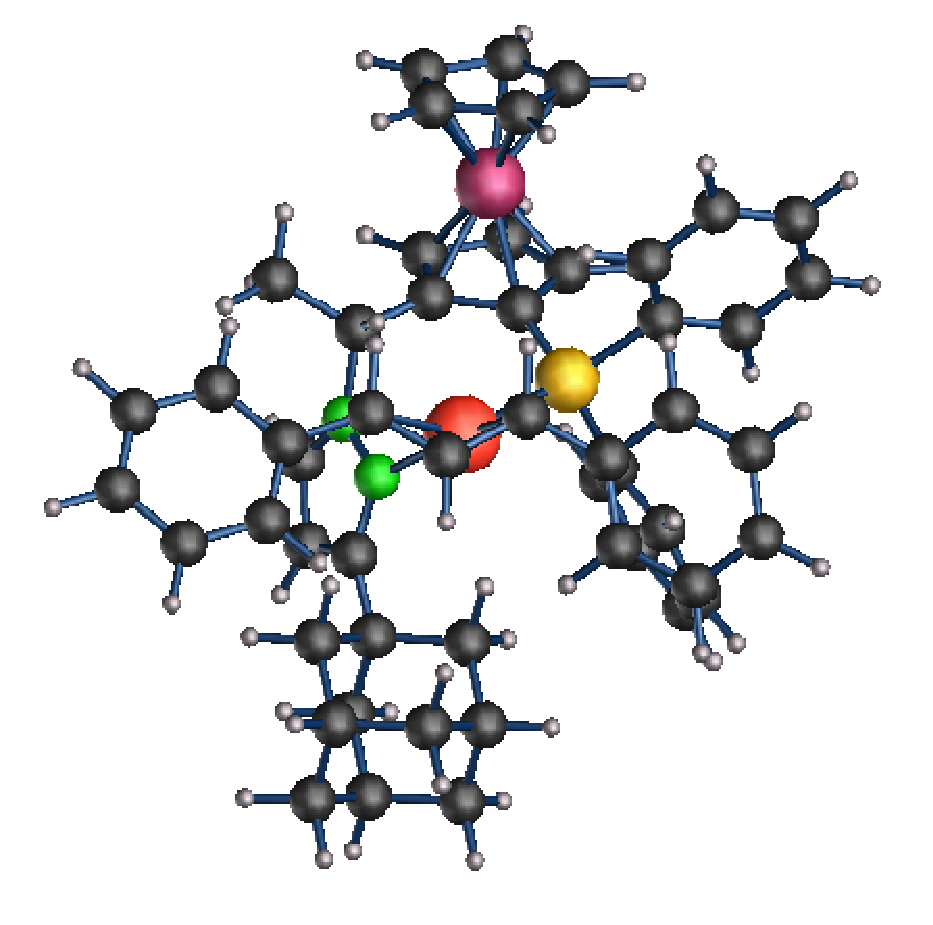
\includegraphics{Figs/big.eps}}
}
\date{\hrulefill\\Peter~E.~Bl\"ochl, Clausthal University of Technology\\(\today)}
%
%==========================================================================
%==                                                                     ===
%==========================================================================
% makeindex makes an index.
% The entries for the index are defined by \index{string}. The index
% is introduced with the latex command \printindex.
% The first run of the compilation produces a file manual.idx. This
% file is processed with the Unix command "makeindex manual.idx",
% which produces a two files manual.ilg and manual.ind.  these will be
% introduces in a second run of the compilation.
\makeindex    


%== allow links between documents ============================================
\usepackage{xr}
\usepackage{xr-hyper}
%==  hyperref package (must be last package)
\usepackage[colorlinks=true]{hyperref} %specify this as last package
\hypersetup{citecolor=blue}
\hypersetup{menucolor=magenta}
\hypersetup{urlcolor=blue}      % 
\hypersetup{filecolor=green}    % file links
\hypersetup{linkcolor=magenta}  %table of contents
\hypersetup{pdfauthor={Peter E. Bl\"ochl}}
\hypersetup{pdfdisplaydoctitle=true}

\begin{document}          
\maketitle
%
\noindent            
\setcounter{page}{1}
\footnote{The title picture shows the a chiral Pd complex with P,N ligands, a
  highly enantio-selective catalyst for allylic amination
  \cite{bloechl96_organometallics15_4125}.}
\newpage
\tableofcontents
%==========================================================================
\newpage
\setcounter{page}{1}
\section{Initial remarks}
%==========================================================================
I am frequently changing the CP-PAW program. Therefore, it is
unavoidable that this description is incomplete in some places,
that it may lists options that are no longer supported, or that it
contains errors. Please let me know if you find something unclear or
even incorrect. Other users will be grateful.

I have attempted to make the program test for inconsistencies of the
input data, such as the selection of conflicting options. You will find
that the program stops in such cases and tries to advise the user
concerning what has gone wrong. New users are particularly creative in
the combinations of options they choose. If you run into problems that
the program does not detect, for example if it crashes without giving
a useful message, please let me know {\em before} you get used to working
around the problem. Your input is particularly valuable in making the
the code more secure to use.

Any other suggestions on how to improve the clarity of this description
or the code are most welcome.

The CP-PAW code including all related material is distributed under
the the GNU Public License V3.

%==========================================================================
\section{What is the projector augmented wave method?}
%==========================================================================
The projector augmented wave method \cite{bloechl94_prb50_17953} is an
all-electron electronic structure method, which allows accurate electronic
structure calculations and ab-initio molecular dynamics simulations on the
basis of density functional theory.

What is all that?

{\bf Density functional theory (DFT)}
\cite{hohenberg64_pr136_864,kohn65_pr140_1133}. Density functional
theory describes the ground state of a many-electron system by electrons that
do not interact other than through an effective potential that depends on the
electron density. It is based on an exact theorem, which specifies that such a
description, based on the electron density rather than on the electronic
many-particle wave function, be rigorously possible for ground states. In
practice the density functional, which also defines the effective potential as
a functional of the density, is not exactly known. However, highly successful
approximations have been found. In contrast to Hartree-Fock calculations,
density functional theory explicitly treats electron correlation. The accuracy
is typically comparable to that of MP2 calculations, i.e. only a few kcal/mol
\cite{becke92_jcp97_9173,dickson93_jcp99_3898}.

{\bf Ab-initio molecular dynamics (AIMD)}
\cite{car85_prl55_2471,car89_bookchapter_455,pastore91_pra44_6334} is an
extension of traditional electronic structure methods which has been invented
in 1985 by Roberto Car and Michele Parrinello \cite{car85_prl55_2471}.  The
best way to think of it is as a series of electronic structure calculations,
one for each time slice, for always different atomic positions. From one time
slice to the next, the atomic positions are changed according to Newton's
equations of motion $M_i\ddot R_i=F_i$.  Here $M_i$ is the mass of a nucleus,
$R_i$ the position, $F_i$ the force acting on the nucleus as calculated from
the electronic structure, and the double-dots stand for the second time
derivative.  Self-consistent iterations at each time step are avoided by a
dynamical evolution of the wave functions, and thus simulations of several
picoseconds are possible, which is sufficient to simulate directly chemical
reactions and diffusion with low barriers or at high temperatures.

Whereas the basic idea of ab-initio molecular dynamics is to perform
real-time and finite temperature simulations, it can be used like a
traditional electronic structure method -- using a friction to
``cool'' the temperature to zero -- and it has been combined
with statistical approaches to study processes with large barriers.

The {\bf projector augmented wave method (PAW)}
\cite{bloechl94_prb50_17953} has been developed in response to the
invention of the ab-initio molecular dynamics approach. Whereas the
latter was based on the plane wave pseudopotential approach, a new
method was needed to enhance the accuracy and computational efficiency
of the approach and to provide the correct wave functions, rather than
the fictitious wave functions provided by the pseudopotential
approach.  The PAW method describes the wave function by a
superposition of different terms: There is a plane wave part, the
so-called pseudo wave function, and expansions into atomic and pseudo
atomic orbitals at each atom. On one hand, the plane wave part has the
flexibility to describe the bonding and tail region of the wave
functions, but used alone it would require prohibitive large basis
sets to describe correctly all the oscillations of the wave function
near the nuclei. On the other hand, the expansions into atomic
orbitals are well suited to describe correctly the nodal structure of
the wave function near the nucleus, but lack the variational degrees
of freedom for the bonding and tail regions.  The PAW method combines
the virtues of both numerical representations in one well-defined
basis set.

Of course, one does not want to make two electronic structure
calculations  -- one using plane waves and one with atomic
orbitals --, and thus double the computational effort. Therefore, the
PAW method does not determine the coefficients of the ``atomic orbitals''
variationally. Instead, they are unique functions of the plane wave
coefficients. It is possible to break up the total energy, and most
other observable quantities, into three almost independent
contributions: one from the plane wave part and a pair of expansions
into atomic orbitals on each atom. The contributions from the atomic
orbitals can be broken down furthermore into contributions from each atom,
so that strictly no overlap between atomic orbitals on different sites
need to be computed.

The PAW method is in principle able to recover rigorously the density
functional total energy, if plane wave and atomic orbital expansions are
complete. This provides us with a systematic way to improve the basis set
errors.  The present implementation uses the frozen core approximation, even
though the general formalism allows extensions in this respect. It provides
the correct densities and wave functions, and thus allows us to calculate
hyperfine parameters etc.  Limitations of plane wave basis sets to periodic
systems (crystals) can easily be overcome by making the unit cell sufficiently
large and decoupling the long-range interactions
\cite{bloechl95_jcp103_7422}. Thus the present method can be used to study
molecules, surfaces, and solids within the same approach.

%==========================================================================
\section{How the code is built}
%==========================================================================

This section is about programming philosophy.  I write this up because
I myself often wonder when I use other software why something is done
in a particular fashion. Therefore, I shall present my reasoning here.
Feel free to skip this section if you wish.

The program is written in an {\bf OO (object-oriented)} manner. This
means that it consists of agents (objects) that perform certain
operations or provide the selected information. Each agent holds the
data needed to perform its job, and it can request the data it needs
from other agents. This is a major software strategy, widely used
today, which allows the programmer to hide certain details, he need
not really worry about at the current level of programming. It also
allows him to assemble the code from little ``boxes'', which are easy
to maintain and enhance.

As part of the OO design, the program uses its own low level object
library, which customizes a number of common operations, such as
interprocessor communication, error handling, file handling,
tree-linked-list structures for intuitive IO, periodic table,
constants, DFT functionals, tracing, timing, string handling, and a
few more. These low-level objects are rather unspecific to the PAW
code, and can be used in combination with self-developed analysis
tools. 

The language used is {\bf FORTRAN 2008}. FORTRAN is itself not an OO
language such as C++ and Java, and thus limits the possibilities in
this respect. However, it has a number of advantages for number
crunching, such as good compilers and, for my taste, a natural and
easily comprehensible way to write mathematics. Compared to FORTRAN77
it is a significant advance towards the OO features of C++ or Java
because it incorporates features such as dynamic memory allocation,
derived data types (structures), operator overloading, modules, etc.
The option of using templates has been implemented using a self-made
preprocessor.  

The program allows {\bf parallel processing} using MPI (Message
Passing Interface) \cite{mpi}. It is (almost) scalable in central
memory and CPU time.  The scalar version program is identical to the
parallel version with the exception that a dummy interface is used
instead of MPI.

The program relies heavily on linear algebra packages such as LAPACK,
BLAS and FFTW. These libraries take care of basic computations such
as matrix multiplications and FFTs (Fast Fourier transforms). A large
fraction of the total CPU time is spent in these routines. In this way
the code development concentrates on algorithmic developments and not,
for example, on how to optimize a FFT.  The latter will be done by
experts who continually adapt this library to modern computer
architectures.

The CP-PAW code is very restrictive in using external libraries. I
have seen some libraries come and go, which is not acceptable for a
code that is supposed to last several decades. (At the time of writing
CPPAW does not use any libraries other than LAPACK, BLAS, FFTW and
MPI.) Even these libraries are connected to the PAW code through a a
set of interface routines, which are collected in two places, one for MPI (\verb|paw_mpelib.f90|) and one for the others \verb|paw_library.f90|. 

One programming principle, I try to follow, is the engineering
motto {\bf ``Fewer Parts!''}. For the user this implies that he will
find few instances where two options provide the same functionality. I
hope that the limitations will be offset by clarity.

The program uses \textbf{Hartree atomic units}\index{Hartree atomic
  units}, that is $\hbar=e=m_e=4\pi\epsilon_0=1$, and Cartesian
coordinates.  Angles are handled in radian ($2\pi{\rm\ rad}=
360~\deg$).  The conversion to other units is often done during
printing. The conversion factors are provided by a particular agent
(see section~\ref{constants}), which is based on the values of
fundamental physical constants recommended by CODATA
(Committee on Data for Science and Technology of the International
Council of Scientific Unions) \cite{mohr00_rmp72_351}.

The program divides work into {\bf three steps: simulation --
  analysis -- visualization}.  The program consists of the simulation
code, which is the core of CP-PAW, and a number of tools used to
analyze the results.  The simulation code calculates energies,
densities, wave functions, trajectories, etc., and writes the
resulting data into files.  These files are then read by tools, which
collect the desired information, and bring it into the desired
form, typically as another file that can be read by your graphics
utilities.

Why this three-layer strategy?

Analysis is both an iterative process and an art: when you find
something interesting, you want to take a closer look quickly with the
tools at hand. Sooner or later, you will probably want to make your
own analysis tools, because you have found a way to understand your
data that nobody has thought of before. Or you want examine a
property, which nobody has tried to calculate. Or you have a unique
visualizer and need an interface for it.  And because you want to
discuss this particular result with your colleagues at the upcoming
coffee break, you choose the quick-and-dirty approach.  You do not
want to do this inside the simulation code, because you dare not
jeopardize its operation.

In contrast to analysis, simulation is computationally expensive.
Therefore, it is desirable to archive as much data from the simulation
as possible, and be able to go back later and look at it again. Hence
the simulation writes most data in machine-readable form (which saves
a considerable amount of disk space).  The data are written in a
simple format so that it is easy to read them into the analysis tools.

Visualization is also separated from analysis, because many tools
exist and the choice is a matter of taste and wealth. The analysis
tools that come with the CP-PAW code will write data formats for the
visualization tools that we currently use.  However, you can easily
change the format to adapt them to your preferred graphics programs.

Of course you can see the most important information, such as total
energies and one-particle energies directly while the simulation is
proceeding. You may also contact other users about further analysis
tools and exchange them. If you wish to write a graphical interface
that hides all three steps from the user, feel free to do so.


%==========================================================================
\section{Input data structure}
%==========================================================================
%
The input data of the simulation code and the tools uses a format
that attempts to be both general and intuitive. Logically, the data
are arranged in a tree structure similar to pull-down menues or
directory trees in unix. It allows one to hide options of the program that
the user may not be interested in, which then can be handled by
default values, and it avoids the unnecessary restrictions of formatted
input. The PAW library has objects that can handle such structures
easily, so that it is widely used for data input for both the
simulation code and the analysis tools. The following section shall
make you familiar with the general layout of input data.
%
%==========================================================================
\subsection{Syntax rules for the input data}
%==========================================================================

Input data are structured as nested data blocks, each identified
by a key word. Each data block may contain other data blocks and
data. Data are again specified by keywords.

The following simple example shall illustrate the structure 
\begin{verbatim}
!FIRSTBLOCK
  DATA=5
  !SECONDBLOCK OTHERDATA=T !END
  !SECONDBLOCK OTHERDATA=F !END
        # this is a comment. The entire line is ignored.
  !THIRDBLOCK_OFF TEXTDATA='THIS IS A TEXT' !END
!END
!EOB
\end{verbatim}
The indentation and the arrangement of the data is arbitrary. The only
requirements are that data and keywords be separated by blanks or
line breaks, and that their sequence observes the logical tree structure
described below.

Lines which begin with hash ($\#$) are ignored while parsing the input
file. This is one mechanism to include
\textbf{comments}\index{comments !input files}. Another one is to add
text beyond the \verb|!EOB|.

Every block starts with a block identifier and ends with the string
``!END''.  The identifier starts with an exclamation mark such as
!FIRSTBLOCK. (Of course one can use any other name instead of
``FIRSTBLOCK''. The recognized block key words are described in the
later sections of this manual.) The last block must be followed by
``!EOB'' (End-Of-Buffer) to indicate the end of all data blocks. Each
block, together with its data and any contained subblocks, can be
made invisible by appending ``\_OFF'' to the block name as done for
!THIRDBLOCK in the example. Data blocks may occur multiply such as
!SECONDBLOCK, if specified in this manual. The order in which the data
blocks are given is irrelevant as long as their hierarchy is observed.
An exception are multiple data or datablocks, where the order in
which they occur may or may not be significant.  Each data refers
only to its block. For example, the two occurrences of OTHERDATA=
are different even though their key words are identical, because they
are within different subblocks.

The general format of input data is a key word, as specified in this
manual separated by an ``='' sign from the input data.  The input data
can be simple data or arrays. Higher dimensional arrays are treated
like in Fortran with the first dimension incremented first, such as
a(1,1)\ a(2,1)\ a(1,2)\ a(2,2). The data are read in free format.
%(The type of the input data is specified in parenthesis following the
%identifying string. If a number is proceeding the type specification it is
%the number of elements to be given. If this number is a "*" details
%are given in the following description for that input data.)

Note that a mistyped key word makes the data or entire branches of the
tree structure invisible. There is no way to warn the user if some key
words have not been recognized.  If the same key word is given several
times in a given data block, without being specified as a multiple,
only the first occurrence is recognized.  The same is true for data
blocks. It is therefore recommended that the protocol be checked to
determine, whether all data have been used as intended.

The type of data is determined as follows:
\begin{itemize}
\item if a data contains a single or double apostrophe, it is
  assumed to be of character type,
\item if a data contains an open parenthesis, it is assumed to be of
  complex type,
\item if a data is either T, F, .true. or .false. it is assumed to be of
  type logical,
\item if a data contains a period it is assumed to be of type real,
\item otherwise, the data is assumed to be of type integer.
\end{itemize}
These rules are checked in the order given here.  It is allowed to
precede a data item by an integer and a multiplication sign such as
$3*0.$, which is shorthand for 0.\ 0.\ 0. (In some cases, one is
allowed to provide both integer and real. Therefore, if you provided a
number of the wrong type and, against your expectation, the program
does not complain, a conversion has been done by rounding the number
to the nearest integer or a simple type conversion from integer to
real has occurred.)

The description uses the following notation. Data blocks are
indicated by a frame. The enclosed name contains the entire
hierarchy of data blocks. Only the last one must be specified on the
date file. However, this data block must be enclosed by the higher
level data blocks. The key words relate to the individual data. If we
cross reference data, we use the entire hierarchy of parent
blocks, followed by a colon and the data keyword.

%
%==========================================================================
\subsection{Extended notation for atoms}
\label{sec:extendedatomnotation}
%==========================================================================
The PAW code refers to atoms by name. No two atoms must be given the
same name. Arbitrary names, given a length limit, are allowed.
However, the recommended notation chooses the first two characters as
the element symbol, with blanks replaced by underscores, and the
remainder is a number. Starting the name with the element symbol
allows to exploit some default settings. The names are defined in the
structure input file and can be referred to in other specifications
and by the PAW tools.

In solids, it will be necessary to distinguish between periodic images
of the same atom. An example is a bondlength constraint between two
atoms, of which one is a periodic image of a original atom. In that
case we use in some cases an extended naming convention.

In the \textbf{extended notation the atom name}\index{extended
  notation atom name}\index{atom name !extended notation} has the form
``\textit{name}:\textit{ijk}'', where {\it name} is the name of the
atom in the original atom cell. and {\it i,j,k} are the three
translations along the lattice vectors. The latter can be single digit
integer numbers with or without preceding sign. To give a few
examples ``H\_2:100'', ``H\_2:+1+0+0'', ``H\_2:10-1''.

Note, that the translations do {\em not} specify a unit cell that
contains that atom. For example, an atom that moves about will never
change its lattice translations, despite traversing several unit
cells. Rather the atoms are considered first as a initial cluster, which forms
a lattice by repetition and lattice translations. There is no
restriction that the atoms of the initial cluster are confined in one
unit cell.

The extended notation will be used increasingly. However, please refer
in all cases to the manual before using the extended notation. It is
also mandatory that original atom names are chosen such that no
confusion can occur. A simple rule that avoids confusion, is not to
use colons in atom names.


%==========================================================================
\newpage
\section{Before starting...}
%==========================================================================
In this manual, I frequently refer to \$PAWDIR and \$ROOT. They are
explained in the following:

%==========================================================================
\subsection{The PAW directory}
%==========================================================================
\$PAWDIR is the name of the directory where the PAW code is
installed. 

In the directory \$PAWDIR you will find the following directories 
\begin{itemize}
\item \verb|src| contains the source codes. The sources for the
analysis tools are located in a subdirectory \verb|Tools|.
\item \verb|doc| contains the manual and installation notes
\item \verb|bin| will be created if it does not exist. It contains the
executable codes
\item \verb|dx| contains files required by the dataexplorer to
visualize wave functions, densities and atomic structures
\end{itemize}



If the program is set up properly, you will have an
environment variable {\tt \$PAWDIR}, which refers to the directory
where the PAW code is installed. You can try it with ``{\tt echo
  \$PAWDIR}'', which will print the PAW directory. Then you can go to
the PAW directory using ``{\tt cd \$PAWDIR}'', and see its contents
using ``{\tt ls -l}''.


%==========================================================================
\subsection{The project data structure}
\label{ROOT}
%==========================================================================
\begin{sloppypar}
All files for a given system should be located in one directory, and
it is recommended that this directory contain only that project.  All
filenames belonging to that system will have a common root, which we
denote in a Unix-like fashion by \$ROOT (the value of the variable
``{\tt ROOT}''). The individual files are distinguished by their
extensions. For example, you can look into the directory ``{\tt
  \$PAWDIR/Sample}''. Here you will find a number of files that begin
with ``{\tt h2co}''. In this case, the root for the filenames (\$ROOT)
is ``{\tt \$PAWDIR/Sample/h2co}''. Note that te root is always
specified by its absolute path. The filenames have extensions of the
kind ``{\tt .cntl}'', ``{\tt .strc}'', ``{\tt .rstrt}'', etc.  Each
extension defines a particular role of the file within the project.
For example, in the file ``{\tt \$ROOT.cntl}'' one defines which
operations the simulation code shall do, in the file ``{\tt
  \$ROOT.strc}'' one defines the molecule or crystal to be studied,
and the file ``{\tt \$ROOT.rstrt}'' holds, among other data, the
instantaneous atomic coordinates and electron wave functions that the
simulation code needs to know in order to continue the simulation.
\end{sloppypar}

You can make exceptions to this rule and define the filenames
explicitly. This may be useful, for example, if you wish to store the
bulkiest file elsewhere, because you have run out of space on the
disk, where you store the projects.

Note that, unlike \$PAWDIR, your environment does not know what \$ROOT
is. Therefore, you should use \$ROOT in this manual as a placeholder for
the full root name, unless the variable ``{\tt ROOT}'' is
explicitly defined. 

%==========================================================================
\section{The simulation code}
%==========================================================================

\subsection{How to perform a simulation}

\subsubsection{Input files}

In order to run the simulation code, two input files have to be
prepared:

\begin{enumerate}
\item The \textbf{structure input file}\index{structure input
  file}\index{input file !structure} (or often simply called STRC),
  describes the system to be studied. Here you provide information
  about which atoms you wish to simulate, what their specifics are,
  whether you wish to simulate a molecule or a crystal and so on.
\item The \textbf{control input file}\index{control input
  file}\index{input file !control} (sometimes abbreviated as CNTL)
  describes what the program shall do, such as optimizing the wave
  functions, relaxing the atoms or simulating at finite temperature.
\end{enumerate}

After the simlation has finished, the program writes a restart file, which
holds the actual wave functions and the positions of the atoms. This
file holds all the necessary information to continue a simulation from
the point where you finished.  It is important to keep the restart file
and the structure file if you wish to return later to what you have
done. 

\subsubsection{Execute the simulation code}

The simulation code is executed using the command

\bigskip\fbox{{\tt paw\_fast.x } {\it controlfile} {\tt 1$>$err 2$>$\&1 \&}}\bigskip

\noindent where {\it controlfile} is the name of the control input
file described in the next section.  With {\tt 1$>$err} one redirects
the print statements to the file out. If the file existed before it is
overwritten. This information is normally irrelevant and is used for
development purposes. However, it is crucial for tracing errors.  With
{\tt 2$>$\&1} one redirects also error messages into the same file,
namely {\tt err}. Thus also error messages be it from PAW or from the
system are written in the same directory. The last {\tt \&} simply
sends the job into the background. That is you can continue working in
the same window while the job is running.

{\tt paw\_fast.x} is simply the name of the PAW executable. There will
be several executables. If you are using a parallel computer using MPI
you will need an executable that starts with {\tt ppaw} instead of
{\tt paw}. The executable with {\tt fast} is the one compiled with all
reasonable optimization flags for the compiler. For all normal
purposes this one should be used. In addition there may be an
executable with {\tt dbg} instead of {\tt fast} for debugging purposes
and one with nothing, with no special flags, which can be used to find
errors induced by optimization.

You can also obtain information about the executable
\begin{center}
\begin{tabular}{ll}
\verb+--help+ & print help information \\
\verb+-h+ & print help information \\
\verb+?+ & print help information \\
\verb+--version+ & print version information\\
\verb+--parmfile+ & print parameter file used for compilation\\
\end{tabular}
\end{center}
The version information shall allow to correlation the executable to a
well-defined version of the source code. The parameter file in
addition provides information about what libraries are linked and
which compilation flags have been used etc. This information is
important to track bugs in the code.

Sometimes it is convenient to write a little wrapper shell-script for
the execution command.
\begin{verbatim}
#!/bin/sh
#===================================================
# sample doit file to execute the simulation code ==
#===================================================
#                                define the rootname 
ROOT=/home/user/Tree/Testrun/H2CO/h2co                               
#                             execute paw simulation
paw_fast.x ${ROOT}.cntl 1>${ROOT}.err 2>&1
\end{verbatim}
This file would be called {\tt \${ROOT}.doit}, which is
also the command to execute the code.  Such a wrapper avoids some
unnecessary typing if you run the job repeatedly. It can easily be
modified to execute the simulation code several times with different
control files.

What does the wrapper do? Let us discuss it line by line. (Comment
lines, i.e. those starting with a hatch sign, are not discussed.)
\begin{enumerate}
\item The first line {\tt \#!/bin/sh} simply specifies that the
  wrapper is a shell script
\item The second line defines a variable {\tt ROOT}. In the following
  commands \${ROOT} is shorthand for {\tt
  /home/user/Tree/Testrun/H2CO/h2co}. Thus one can use the same
  wrapper for different simulations by simply changing the value of
  {\tt ROOT}.
\begin{sloppypar}
  The last line executes the the simulation code using the control
  file {\tt \${ROOT}.cntl}. 
\end{sloppypar}
\end{enumerate}

In order to track the simulation one can issue the command

\bigskip\fbox{{\tt tail -f \$ROOT.prot }}\bigskip

which continually prints the lines written to the protocol file also
to the screen. Another way to trace the simulation is the command {\tt
paw\_show} described in section~\ref{sec:pawshow}.


\subsubsection{Terminate the simulation}

The execution can be stopped before regular completion by creating a
so-called exit file

\bigskip\fbox{{\tt touch }{\it exitfile}}\bigskip

\noindent where {\it exitfile} is the name of the exit file. 
The standard name is \$ROOT{\tt .exit}, but this name can be changed
in the control input file.

As an alternative to setting the exit file, the CP-PAW code also contains
a signal trap. The command

\bigskip\fbox{{\tt kill -30\ }{\it PID}}\bigskip

\noindent where {\it PID} is the process id number, causes the program
to terminate the execution after the next iteration. Note, however,
that this command can sometimes crash the code, namely if the code is
writing to a file at the moment you issue the command.  Its use is
therefore not recommended, and it may even be removed from future
versions. The process id number can be obtained either from the
command \verb|top| or from the command \verb+ps -elf |grep paw+.

%
%==========================================================================
\subsection{The control input file ``CNTL''}
%==========================================================================

The control file is responsible for ``what to do'' in the
simulations. These data are generally unspecific to the system.

%==========================================================================
\subsubsection{Examples for the control input file ``CNTL''}
%==========================================================================
The following is a particularly simple example for a control input
file. This file can be used for getting started.

\begin{verbatim}
!CONTROL
  !GENERIC START=T NSTEP=100 !END   
  !FOURIER EPWPSI=30 CDUAL=2 !END
  !PSIDYN  
    !AUTO FRIC(+)=0.3 FACT(+)=1. 
          FRIC(-)=0.3 FACT(-)=0.97 !END
  !END
!END         
!EOB
\end{verbatim}

The following example illustrates a few more options that give a quick
impression of the choices available. The detailed description of all
options is given in the next section.

\begin{verbatim}
!CONTROL
 !GENERIC START=T DT=10 NSTEP=100 NWRITE=100 !END   
 !DFT     TYPE=2 !END
 !FOURIER EPWPSI=30 CDUAL=2 !END
 !PSIDYN  STOP=T FRIC=0.005 RANDOM=0.1 
          MPSI=1000 MPSICG2=0.5 
   !AUTO  FRIC(-)=0.3 FACT(-)=0.97 
          FRIC(+)=0.5 FACT(+)=0.97 !END
   !THERMOSTAT_OFF STOP=T FRIC=0 
          T[K]=100 FREQ[THZ]=10 !END 
 !END
 !RDYN    STOP=T FRIC=0 RANDOM[K]=0 
   !AUTO  FRIC(+)=0.5 FACT(+)=0.97 
          FRIC(-)=0.3 FACT(-)=0.97 !END
   !THERMOSTAT_OFF STOP=T FRIC=0 
          <EKIN>=0.02 FREQ[THZ]=50 !END
 !END
 !FILES
   !FILE  ID='EXIT' EXT=F NAME='~/EXIT' !END
 !END
 !ANALYSE 
   !HYPERFINE ATOM='H_1' EFG=T ISOMERSHIFT=T 
              FERMICONTACT=T ANISOTROPIC=T   !END
   !DENSITY FILE='./density.ev' TYPE='TOTAL' 
         DR=0.4 OCC=T DIAG=T CORE=F !END
   !WAVE FILE='./wavefunction.wv' 
         DR=0.4 B=10 K=1 S=1 IMAG=F !END
   !POTENTIAL FILE='./potential.wv'
         dr=0.4 !END
 !END
!END
!EOB
\end{verbatim}

%==========================================================================
\subsubsection{Argument keywords for the control input file ``CNTL''}
%==========================================================================

%----------------------------------------------------------------------
\block{!CONTROL}
%----------------------------------------------------------------------
\brules{optional}
\bdescr{defines the operations performed on the system; 
largely independent of the system}

%----------------------------------------------------------------------
\block{!CONTROL!FILES}
%----------------------------------------------------------------------
\brules{optional}
\bdescr{specifies the file names that deviate from the standard values}

\mbax{\key{ROOT}
\vdescr{rootname. Files defined as extension will have this name
  combined with the extension. All files connected as default are
  defined as extensions.}
\vformat{character}
\vrules{optional}
\vdefault{string preceding the '.cntl' ending of the control input file}}

%----------------------------------------------------------------------
\block{!CONTROL!FILES!FILE}
%----------------------------------------------------------------------
\brules{optional, multiple}
\bdescr{Specifies one file}

\newpage
\mbax{\key{ID}
\vdescr{identifier for the file; options are:\hfill\break 
\noindent
\begin{tabular}{|l|l|}
\hline
'PROT'& protocol; extension:{\tt .prot}\\
&monitors the simulation.\\
\hline
'STRC'& structure input file; extension:{\tt .strc}\\
& defines atoms, structure, electron \\
&occupations etc.\\
\hline
'CNTL'& control input file; extension:{\tt .cntl}\\
&used to control the simulation.\\
\hline
'PARMS\_STP'& setup parameter file; \\
&default: {\tt \$PAWDIR/parameters/stp.cntl}\\
&defines the parameter sets for the augmentation.\\
\hline
'RESTART\_IN'& input restart file; extension {\tt .rstrt}\\
&instantaneous coordinates\\
\hline
'RESTART\_OUT'& output restart file; extension {\tt .rstrt}\\
&see 'RESTART\_IN'\\
\hline
'EXIT'& exit file; extension: {\tt .exit}\\
& simulation terminates if exit file exists\\
\hline
'PDOS'& projected density of states;\\
& extension: {\tt .pdos}\\
& used by the paw\_dos tool\\
& generated by the main paw program.\\
\hline
'PDOSOUT'& projected density of states;\\
& extension: {\tt .pdosout}\\
& used by the paw\_dos tool.\\
& generated by the paw\_bands tool.\\
\hline
'BANDDATA'& paw hamiltonian for band structure;\\
& extension: {\tt .banddata}\\
& used by the paw\_bands tool.\\
\hline
'CONSTRAINTS'& constraint report;\\
& extension: {\tt \_constr.report}\\
\hline
'POSITION\_TRAJECTORY'& atomic positions; 
extension {\tt \_r.tra}\\
&trajectory used by the paw\_tra tool.\\
\hline
'BANDS\_TRAJECTORY'& one-particle energies;\\
&extension {\tt \_r.tra}\\
&(not yet used)\\
\hline
'AUGPARMS'& parameter sets for the augmentation;\\
&extension: no default extension\\
\hline
\end{tabular}
}
\vformat{character} 
\vrules{mandatory}
\vdefault{none}}

\mbax{\key{NAME}
\vdescr{filename. Can be the relative file name or an extension to the
  PAW ``root''. Standard output can be specified by NAME='stdout'
  and EXT=.false.}
\vformat{character} 
\vrules{mandatory}
\vdefault{none}}

\mbax{\key{EXT}
\vdescr{.true.: NAME specifies the extension only/ .false.: full name}
\vformat{logical}
\vrules{optional}
\vdefault{.false.}}

%----------------------------------------------------------------------
\block{!CONTROL!GENERIC}
%----------------------------------------------------------------------
\brules{optional}
\bdescr{general data that do not fit into other blocks}

\mbax{\key{START}
\vdescr{T: start with random wave functions, and atomic positions from file 
"STRC"\hfill\break 
F: wave functions and atomic positions are taken from restart file, 
unless specified otherwise}
\vformat{logical}
\vrules{optional}
\vdefault{F}}

\mbax{\key{NSTEP}
\vdescr{number of time steps}
\vformat{integer}
\vrules{optional}
\vdefault{100}}

\mbax{\key{DT}
\vdescr{time step $\Delta$ in a.u. (1~a.u.$\approx$ 0.024~fs)}
\vformat{real}
\vrules{optional}
\vdefault{10.0}}

\mbax{\key{NWRITE}
\vdescr{Every ``NWRITE'' time steps, the program writes detailed information 
into the protocoll file and it updates the restart file. Note that writing 
the restart file is time consuming.}
\vformat{integer}
\vrules{optional}
\vdefault{100}}

\mbax{\key{TRACE}
\vdescr{provides trace information when entering or leaving
subroutines under trace control. Used for debugging purposes.}
\vformat{logical}
\vrules{optional}
\vdefault{.false.}}

\mbax{\key{ENDIAN} \vdescr{defines whether unformatted files are
written in little endian as typical on Intel computers or in big
endian as on IBM computers. The value can be
'little','intel','big','ibm'. The first two values have identical
meaning and the last two have identical meaning.
It is only functional using certain compilers (Absoft).}  
\vformat{character}
\vrules{optional} \vdefault{little}}

\mbax{\key{RUNTIME} 
\vdescr{A soft stop is initialized after the given time has elapsed
since start of the code.  Runtime is specified as a three element
vector containing (hours,minutes,seconds). The three elements of the
vector are internally converted into seconds and added up.}
\vformat{integer} 
\vrules{optional} 
\vdefault{$\infty$}}

\mbax{\key{AUTOCONV} 
\vdescr{The autopilot defines a strategy to vary
the friction for various dynamical variables, to test the convergence
and to terminate the optimization loop. The decision to terminate is
taken if the energy remains within an energy window of size ETOL for
autoconv time steps.}
\vformat{integer} 
\vrules{optional} 
\vdefault{20}}

\mbax{\key{ETOL} 
\vdescr{The autopilot defines a strategy to vary
the friction for various dynamical variables, to test the convergence
and to terminate the optimization loop. The decision to terminate is
taken if the energy remains within an energy window of size ETOL for
AUTOCONV time steps.}
\vformat{integer} 
\vrules{optional} 
\vdefault{$10^{-8}$~H}}

\mbax{\key{RSTRTTYPE} \vdescr{allows to cut down the information on
the restart file.  Option RSTRTTYPE='STATIC' only stores one set of
wave functions. This reduces the amount of disk space by nearly a
factor of two. This option should not be used in a dynamical
simulation, because, the velocity of the wave functions will be set to
zero.}
\vformat{character}
\vrules{optional}
\vdefault{NONE}}

\mbax{\key{NEWSTRC} 
\vdescr{Unit cell and atomic positions from
    structure input file overwrite any structure information from
    restart file.}
\vformat{logical}
\vrules{optional}
\vdefault{F}}

%----------------------------------------------------------------------
\block{!CONTROL!DFT}
%----------------------------------------------------------------------
\brules{optional}
\bdescr{selects density functional parameterization; default is Perdew-Zunger
parameterization of the Ceperly-Alder quantum Monte-Carlo calculation}

\mbax{\key{TYPE} 
  \vdescr{density functional parameterization.
    possible values are:\hfill\break 
    
    {\bf(1)} Perdew-Zunger parameterization \cite{perdew81_prb23_5048} of
    Ceperley-Alder \cite{ceperley80_prl45_566}; 
    
    {\bf(2)} Perdew-Wang 91 parameterization \cite{perdew92_prb45_13244} of
    Ceperley-Alder \cite{ceperley80_prl45_566}; 
    
    {\bf(3)} Local exchange (X$_\alpha$ with $\alpha$=2/3); 

    {\bf(4)} X-alpha (alpha=0.7); 
    
    {\bf(6)} Local exchange and Becke gradient correction
    \cite{becke88_pra38_3098} for exchange; 
    
    {\bf(7)} Perdew-Wang LSD \cite{perdew92_prb45_13244} 
     and Becke gradient correction for
    exchange \cite{becke88_pra38_3098}; 
    
    {\bf(71)} Perdew-Zunger\cite{perdew81_prb23_5048} and Becke-88 gradient
    correction\cite{becke88_pra38_3098};
      
    {\bf(8)} like (7) + Perdew-86 gradient correction for correlation
    \cite{perdew86_prb33_8822};
      
    {\bf (81)} Perdew-Zunger\cite{perdew81_prb23_5048} + Becke gradient
    correction\cite{becke88_pra38_3098} + Perdew86 gradient correction for
    correlation\cite{perdew86_prb33_8822};
    
    {\bf(9)} like (7) + Perdew-Burke Ernzerhof correlation \cite{perdew96_prl77_3865};

    {\bf(10)} Perdew-Burke-Ernzerhof (PBE)exchange and correlation
    \cite{perdew96_prl77_3865}; Almost identical to PW91
    GGA\cite{perdew92_prb46_6671} but simpler formulation.

    {\bf(-10)} like TYPE=10 but with a changed parameter used previously;

    {\bf(11)} RPBE exchange and correlation, includes Hammer's
              correction\cite{hammer99_prb59_7413} to Perdew-Burke-Ernzerhof
              exchange and correlation \cite{perdew96_prl77_3865};} 
\vformat{integer}
\vrules{optional, incompatible with LIBXC} 
\vdefault{10 (PBE functional)}
}

\mbax{\key{LIBXC} 
   \vdescr{density functional parameterization through
    LibXC.  array of functional id's. Typicaly there are one or two
    strings.  See appendix~\ref{sec:libxcids} on
    p.~\pageref{sec:libxcids}.
  %% \begin{center}
  %% \end{center}
}
\vformat{character array}
\vrules{optional, incompatible with TYPE}
\vdefault{see TYPE}
}


\mbax{\key{VDW}
\vdescr{Adds van der Waals Interactions\cite{grimme10_jcp132_154104}. 
The van der Waals interaction is described by an interatomic pair potential 
that has a long-ranged $r^{-6}$ behavior and which is cut of smoothly 
at short distances.}
\vformat{logical}
\vrules{optional (Untested)}
\vdefault{F}}

\mbax{\key{VDW-3BODY} 
\vdescr{adds three-body interactions\cite{grimme10_jcp132_154104} to
    the pair-wise van der Waals interactions of Grimme et al. (As of
    March 2012, not yet recommended by Grimme)}
\vformat{logical} 
\vrules{optional, only used when VDW=T,  (Untested)} 
\vdefault{F}}


%----------------------------------------------------------------------
\block{!CONTROL!DFT!NTBO}
%----------------------------------------------------------------------
\brules{optional} \bdescr{Experimental option. Do not use!  Constructs
  wave function representation in natural tight-binding orbitals.
  Enables to add the additional terms for the hybrid functionals or
  the interface for a solver for the dynamical mean-field theory.}

\mbax{\key{MODUS} 
%
\vdescr{switch between different energy contributions. May be 'HYBRID'
  or 'DMFT'.}
%
\vformat{character} 
\vrules{optional} 
\vdefault{'HYBRID'}}

\mbax{\key{OFFSITE} 
%
\vdescr{Calculates off-site U-tensor. OFFSITE=T is only compatible
  with MODUS='HYBRID'. To be come active, 
  the specific options NDDO, 31 and/or BONDX need to
  be selected for each species in the structure file. 
  See !STRUCTURE!SPECIES!NTBO.}

%
\vformat{logical} 
\vrules{optional} 
\vdefault{false}}

%% \mbax{\key{HFWEIGHT} 
%% %
%% \vdescr{Mixing Factor for replacement of the Fock term.}
%% %
%% \vformat{real} 
%% \vrules{optional} 
%% \vdefault{0.25}}

\mbax{\key{K2} 
%
\vdescr{K2=2 Ekin[H] of the envelope function. The bare Hankel
  function decay faster with decreasing k2.}
%
\vformat{real} 
\vrules{optional} 
\vdefault{-0.25}}

\mbax{\key{SCREENL[AA]} 
\vdescr{The Coulomb interaction in the Exchange term is replaced by a
  Yukawa potential with the specified screening length.  Screening
  length $\lambda$ in {\AA}: The Coulomb interaction in the explicit
  Hartree-Fock term is replaced by a Yukawa potential
     \begin{eqnarray}
     v(\vec{r})=\frac{1}{4\pi\epsilon_0|\vec{r}|}
     \exp\left(-\frac{|\vec{r}|}{\lambda}\right)
     \end{eqnarray}
     in the spirit of the random-phase approximation (RPA),
     respectively the screened Coulomb interaction in GW.  The
     (unscreened) Poisson equation is used, if this parameter is not
     specified. Warning: values below 0.02 are reset to internally to
     0.02 to avoid numerical problems in library routine.}
\vformat{real, $\ge0$} 
\vrules{optional} 
\vdefault{$\infty$}}

\mbax{\key{SCALERCUT} 
%
\vdescr{Atom pairs are included in the neighborlist for structure
  constants, if their distance is less than the sum of covalent radii
  multiplied with SCALERCUT. (The covalent radius of an empty sphere
  is set to 1~a$_0$.}
%
\vformat{real} 
\vrules{optional} 
\vdefault{2.}}

%----------------------------------------------------------------------
\block{!CONTROL!FOURIER}
%----------------------------------------------------------------------
\brules{optional} \bdescr{Plane wave cutoffs
  $E_{PW}=\frac{1}{2}G_{max}^2$ for wave functions and charge density.
  A cutoff of 30~Ry=15~H for the wave function and CDUAL=2 is
  sufficient for most applications. In order to account for all plane
  wave components in the density, the plane wave cutoff for the
  density should in principle be four times the cutoff for the wave
  function.  (For low cutoffs, even CDUAL$>$4 may be required since
  the exchange and correlation functional is nonlinear, and therefore
  the energy may not necessarily decrease monotonically as the
  basis set size is increased with a fixed CDUAL. In practice this is
  rarely a problem.)}

\mbax{\key{EPWPSI} 
%
\vdescr{plane wave cutoff for the wave functions in
    Rydberg (1~Ry=0.5~a.u.). All plane waves up to a maximum
    kinetic energy equal to the plane wave cutoff are considered. Note
    that the plane wave cutoff refers only to the plane wave part of
    the basis functions.}
%
\vformat{real} 
%
\vrules{optional} 
%
\vdefault{30.}}

\mbax{\key{EPWRHO}
\vdescr{plane wave cutoff for the charge density in Rydberg (1~Ry=0.5~a.u.)}
\vformat{real}
\vrules{optional}
\vdefault{4*EPWPSI}}

\mbax{\key{CDUAL}
\vdescr{EPWRHO=CDUAL*EPWPSI; The default cdual=4 produces the correct
result; cdual=2 is often a good choice.}
\vformat{real}
\vrules{optional; this value is overwritten by any occurence of ``EPWRHO''}
\vdefault{4}}

\mbax{\key{EPWBUCKET} 
\vdescr{Used mostly for cell dynamics. 
See section~\ref{sec:sawtooth} for an explanation of the sawtooth 
behavior. The parameter $E_B$ in Ry is specified as
follows: If specified, an additional potential-energy term
$\sum_{G,n}f_n\langle\tilde\Psi_n|G\rangle B(G)\langle
G|\tilde\Psi_n\rangle$, is added to the total energy, where
$B(G)=c_B\theta(\frac{1}{2}G^2-E_B)(G-\sqrt{2E_B})^2$.  When this term
is set to a fixed value, the plane-wave convergence is artificially
accelerated, which is important to evaluate stresses.  The energy
converged this way differs from that converged without this term.
Rather, it corresponds roughly to the total energy
obtained with a plane wave cutoff slightly higher than EPWBUCKET.
Example: $E_{PW}=50$~Ry, $E_B=30$~Ry, $c_B=1$}
\vformat{real} 
\vrules{optional;mandatory of BUCKETPAR is specified}
\vdefault{none}}

\mbax{\key{BUCKETPAR}
\vdescr{Parameter $c_B$ see also description of EPWBUCKET above.}
\vformat{real}
\vrules{optional; mandatory, if EPWBUCKET is specified}
\vdefault{0.}}



%----------------------------------------------------------------------
\block{!CONTROL!PSIDYN}
%----------------------------------------------------------------------
\brules{optional; default uses default values for the electron
  dynamics.} 
\bdescr{Parameters used to control the dynamics of the wave functions.
  The wave function dynamics is governed by the equation $$m_\Psi
  \vert\ddot{\tilde\Psi}_n\rangle = - {{\partial
      E}\over{\partial\langle\tilde\Psi_n\vert}} -
  m_\Psi\vert\dot{\tilde\Psi}_n\rangle \alpha -
  \sum_m\vert\tilde\Psi_m\rangle\Lambda_{mn}, $$
  where $\alpha$ can be
  tuned by a Nos\'e thermostat or the parameters below. The equation
  of motions are integrated using the Verlet algorithm \cite{verlet67_pr159_98}.
  The friction parameter $\alpha$ is converted into a parameter
  $c_\alpha= \alpha\Delta/2$, which can range from 0 to 1.  A value of
  $c_\alpha=0$ indicates frictionless dynamics, whereas a value of
  $c_\alpha=1$ indicates steepest descent. $\Delta$ is the time step.
  A discussion of the virtues of friction dynamics can be found in
  Ref. \cite{tassone94_prb50_10561}}
\mbax{\key{STOP}
\vdescr{if STOP=true start with zero velocity of the wave functions}
\vformat{logical}
\vrules{optional}
\vdefault{F}}

% not implemented in the new version
%\mbax{\key{RANDOM}
%\vdescr{amplitude of randomization of the velocities of the electronic wave 
%functions before the first iteration.}
%\vformat{real}
%\vrules{optional}
%\vdefault{0.}}

\mbax{\key{MPSI}
\vdescr{mass $m_\Psi^0$ for the wave function dynamics. The wave function 
mass is an operator of the form
\begin{eqnarray*}
\hat{m}_\psi=\sum_{\vec{G}} |\vec{G}\rangle 
m_\psi^0(1+c \vec{G}^2)\langle\vec{G}|
\end{eqnarray*}
The coefficient $c$ is set in MPSICG2. 

The G-dependent wave function mass is used to reduce the otherwise
very large frequency of the wave function components with large
$|\vec{G}|$. For the large G-components of the auxiliary wave
functions we can approximate the effective potential by a constant, 
which makes the Hamiltonian diagonal in $|\vec{G}\rangle$. This allows 
to estimate the frequency from
\begin{eqnarray*}
\hat{m}_\psi^0(1+c \vec{G}^2) \ddot\Psi_G
=\left[\frac{\vec{G}^2}{2}+v_{eff}\right]\Psi_G
\end{eqnarray*}
 }
\vformat{real}
\vrules{optional}
\vdefault{10 $\Delta^2$ (for $\Delta$ see "!CONTROL!GENERIC:DT")}}

\mbax{\key{MPSICG2} 
\vdescr{high-G enhancement $c$ for the
    wavefunction mass. The fictitious electron mass for the wave
    function dynamics is G-dependent $m_\Psi(G)=m_\Psi(1+c G^2)$. A
    recommended value is $c=0.5$. A reasonable value is
    $\frac{1}{2}(\frac{x}{2\pi})^2\frac{\Delta^2}{m_\Psi}$, where $x$
    is the fraction of shortest oscillation period for the electron
    dynamics and the time step. The stability criterion of the Verlet
    algorithm requires $x>3$. The default uses this expression with
    $x=10$. For proper mass renormalization (discounting the nuclear
    mass by the effective mass of the wave function cloud) the values
    of !STRUCTURE!SPECIES:PS$<$G2$>$ and !STRUCTURE!SPECIES:PS$<$G4$>$
    need to be specified.}  
\vformat{real} 
\vrules{optional}
\vdefault{$\frac{1}{2}(\frac{10}{2\pi})^2\frac{\Delta^2}{m_\Psi}$}}

\mbax{\key{FRIC}
\vdescr{constant friction $c_\alpha$ for the wave function dynamics}
\vformat{real}
\vrules{optional, not used if ``!CONTROL!PSIDYN!AUTO'' is selected.}
\vdefault{0.0}}


\mbax{\key{SAFEORTHO} 
  \vdescr{chooses the way the orthogonality constraints for the wave
    functions is enforced. If SAFEORTHO=T is selected the traditional
    way is used, which results in a strictly energy-conserving
    dynamics. If SAFEORTHO=F a new method is used which converges at
    eigenstates of the Hamiltonian, but is energy conserving only if
    the states are sufficiently close to eigenstates. This option
    allows to calculate excited states or to treat metals.

    The option ``SAFEORTHO=F''  can artificially stabilize the
    calculation with states is in the ``wrong'' order, i.e. with
    occupations that are not monotonically decreasing. Since the wrong
    order corresponds to a saddle point of the total energy, the wave
    functions accelerate to reach the correct order. This behavior can
    also occur, if the two states that are mis-ordered are both
    occupied or both unoccupied. In that case the energy increases
    temporarily as the wavefunctions acquire kinetic energy, while the
    DFT total energy remains approximately constant. The
    ``zentrifugal'' forces of the wave function dynamics also perturb
    the DFT total energy, so that also the latter increases
    temporarily. Rarely, this behavior can also lead to a instability,
    namely when the energy-levels shift in such a way that the final
    state is again in the incorrect order.}
  \vformat{logical} 
  \vrules{optional} 
  \vdefault{T}
}

\mbax{\key{STRAIGHTEN} 
  \vdescr{Transform the wave functions onto energy eigenstates. The
    transform is performed during the first big writeup of the
    protocoll file. A unitary transform among the wave function is
    performed. That is, the Hilbert space remains unchanged.  Note,
    that the occupations may be inconsistent with the new states. It
    may be advisable to simultaneously restart the occupations.
 
    This option can be used to accelerate convergence with
    !CONTROL!PSIDYN:SAFEORTHO=F, because it shortcuts the lengthy
    dynamics towards energy eigenstates. It may also be useful in the
    early stages of the wave function optimization.
    The abrupt change of the wave functions can upset a nearly 
    converged calculation.}
  \vformat{logical} 
  \vrules{optional} 
  \vdefault{F}
}

\mbax{\key{SWAPSTATES}
\vdescr{\textbf{Experimental option! You are on your own!}
Only used with SAFEORTHO=F. For SWAPSTATES=F, the approximate
eigenstates are ordered in increasing energy expectation values. This
is used for optimizing electronic and atomic structures. Thus the
given occupations refer to increasing one-particle energies in the
final state.

If, in a photochemical reaction with a state crossing with fixed
occupations, the system shall remain on the upper branch of the energy
surface, choose SWAPSTATES=F. If the system shall follow the crossing
to the lower branch of the energy surface, choose  SWAPSTATES=T.

In combination with the Mermin functional the following happens at a
band crossing at the Fermi level.
\begin{itemize}
\item SWAPSTATES=F: the wave functions change their character, which
results in wave function heating. The time scale of the conversion of
the state depends on matrix elements and on the fictitious mass of the
wave functions. This process is therefore rather uncontrolled. The
occupations remain approximately constant. The crossing is treated
like an avoided crossing.
\item SWAPSTATES=T: the wave function maintains its character, but the
occupations dynamically change from occupied to unoccupied and vice
versa. If the crossing is an avoided crossing, the wave functions are
reordered only if the if the conversion of the character of the wave
functions is sufficiently retarded, that a band crossing of the
one-particle energies takes place.
\end{itemize}}
  \vformat{logical} 
  \vrules{optional, not tested}
  \vdefault{F}}  

%\mbax{\key{DIAG}
%\vdescr{apply unitary transformation to the trajectory so 
%that approximate eigenstates are obtained}
%\vformat{logical}
%\vrules{optional}
%\vdefault{.false.}}

% \mbax{\key{STOREPSIR}
% \vdescr{T: store real space wave functions to save cpu time\hfill\break 
% F: recalculate real space wave functions to increase accuracy and
% reduce memory requirements}
% \vformat{logical}
% \vrules{optional}
% \vdefault{T}}

%----------------------------------------------------------------------
\block{!CONTROL!PSIDYN!AUTO}
%----------------------------------------------------------------------
\brules{optional} \bdescr{Automatic annealing procedure for wave
  function dynamics.  (overwrites setting of !CONTROL!PSIDYN:FRIC.)
  For optimizing the electronic structure the default set has been
  proven very useful. The friction switches between a lower and an
  upper value depending on whether the energy decreases or increases.
  The upper and lower friction values are each scaled in each time
  step.  With this option, the program will stop if the total energy
  changes during 20 iterations by less than 10$^{-5}$ Hartree. This does
  not necessarily imply convergence of the annealing step. It can
  happen, in particular near convergence, that the friction jumps from
  step to step between the lower and the upper value. In this case the
  system is not converged, even if the total energy is virtually
  constant, and a constant friction should be used.}

\mbax{\key{FRIC(-)}
\vdescr{start value for the friction factor $c_\alpha$ used for
decreasing energy}
\vformat{real}
\vrules{optional}
\vdefault{0.3}}

\mbax{\key{FACT(-)}
\vdescr{factor multiplied with the friction factor FRIC(-) in 
each step that reduces the energy}
\vformat{real}
\vrules{optional}
\vdefault{0.97}}

\mbax{\key{FRIC(+)}
\vdescr{start value for the friction factor $c_\alpha$ used for
increasing energy}
\vformat{real}
\vrules{optional}
\vdefault{0.3}}

\mbax{\key{FACT(+)}
\vdescr{factor multiplied with the friction factor FRIC(+) in 
each step that reduces the energy}
\vformat{real}
\vrules{optional}
\vdefault{1.0}}

\mbax{\key{MINFRIC}
\vdescr{minimum friction used}
\vformat{real}
\vrules{optional}
\vdefault{0.}}

%----------------------------------------------------------------------
\block{!CONTROL!PSIDYN!THERMOSTAT}
%----------------------------------------------------------------------
\brules{optional} \bdescr{Thermostat for the wave
  functions.\cite{bloechl02_prb65_104303} This thermostat shuffles
  energy from the wave functions to the atomic motion, when the
  wave-function kinetic energy former exceeds an estimated target
  value $\frac{1}{2}\sum_iK_i\dot{\vec{R}}_i^2$. A friction on the thermostat
  shall be used to avoid instabilities. The thermostat shall be used
  only if the atoms are moving.
\begin{eqnarray*}
M_i\ddot{\vec{R}}_i&=& \vec{F}_i+K_i\dot{\vec{R}}_i\dot{x}_\psi
\\
Q_\psi\ddot{x}_\psi&=&2\theta(\dot{x}_\psi)
\left(\sum_n f_n 
\langle\dot{\tilde{\psi}}_n|m_\psi|\dot{\tilde{\psi}}_n\rangle
-\frac{1}{2}\sum_i\vec{K}_i\dot{R}_i^2\right)
\end{eqnarray*}
The values for $K_i$ are derived from the atomic pseudo wave
functions.

}

%% \mbax{\key{$<$EKIN$>$}
%% \vdescr{average kinetic energy of the wave functions. Do not use in
%%   the new version.}
%% \vformat{real}
%% \vrules{optional}
%% \vdefault{0.01}}

%% \mbax{\key{T[K]}
%% \vdescr{New version: atom temperature in Kelvin.
%% \\ 
%% Old version: average kinetic energy of the wave functions divided by
%%   Boltzmann's constant. }
%% \vformat{real}
%% \vrules{optional}
%% \vdefault{see $<$EKIN$>$}}



\mbax{\key{PERIOD}
\vdescr{Oscillation period of the Nos\'e variable in a.u.}
\vformat{real}
\vrules{optional}
\vdefault{see !CONTROL!PSIDYN!THERMOSTAT:FREQ[THz]}}

\mbax{\key{FREQ[THZ]}
\vdescr{Frequency of the Nos\'e variable in THz.}
\vformat{real}
\vrules{optional; not used if !CONTROL!PSIDYN!THERMOSTAT:PERIOD present}
\vdefault{100.}}

\mbax{\key{FRIC}
\vdescr{Friction acting on the  Nos\'e variable. Can have values
  between zero and one. The largest value before overdamping is
  $\frac{4\pi}{period}$, where period is that of the thermostat
  variable defined in this section.}
\vformat{real}
\vrules{optional}
\vdefault{0.}}

\mbax{\key{STOP}
\vdescr{set velocity for Nos\'e variable to zero in the first iteration}
\vformat{logical}
\vrules{optional}
\vdefault{F}}

%----------------------------------------------------------------------
\block{!CONTROL!RDYN}
%----------------------------------------------------------------------
\brules{optional; default is fixed atomic positions}  
\bdescr{parameters used to control the
  dynamics of the atomic positions.  The atomic dynamics is governed
  by the equation
  $$M_R \ddot R = - {{\partial E}\over{\partial R}} - M_R\dot R
  \alpha, $$
  where $\alpha$ can be tuned by a Nos\'e thermostat or the
  parameters below.  The friction parameter $\alpha$ is converted into
  a parameter $c_\alpha= \alpha\Delta/2$, which can range from 0 to 1.
  A value of $c_\alpha=0$ indicates frictionless dynamics, whereas a
  value of $c_\alpha=1$ indicates the steepest descent. $\Delta$ is
  the time step.
  \\
  Remark: Do not use this option before the wave functions are
  optimized, because unreasonable forces will result from an incorrect
  electron distribution.}
%
\mbax{\key{STOP}
\vdescr{start with zero velocity for the atomic positions }
\vformat{logical}
\vrules{optional}
\vdefault{F}}
%
\mbax{\key{START}
\vdescr{Take initial structure from structure control file instead
  of the restart file.}
\vformat{logical}
\vrules{optional}
\vdefault{F}}
%
\mbax{\key{RANDOM[K]} 
\vdescr{adds random velocities once at the beginning of the
  simulation; the velocity distribution corresponds to a temperature
  in Kelvin. Can be used to bring the system quickly to a finite
  temperature. Note, however, that the electron wave functions cannot
  immediately follow this sudden kick. They will start to lag behind,
  and deviate from the Born-Oppenheimer surface. A small friction
  acting on the wave functions will allow the wave functions to
  recover. Remark: The initial temperature typically drops quickly,
  because much of the kinetic energy from the initial kick is
  converted into potential energy. For a harmonic oscillator, as model
  for the atomic vibrations, kinetic energy and vibrational potential
  energy become equal in thermal equilibrium. Remark: The random kick
  is reproducible, if the internal (hard-wired) parameter
  \texttt{tsetseed=.true.} in \texttt{paw\_atoms.f90}. This is useful for
  testing, but it may conflict sampling over different trajectories.}
  \vformat{real} 
  \vrules{optional} 
  \vdefault{0}}

\mbax{\key{FRIC}
\vdescr{constant friction $c_\alpha$}
\vformat{real}
\vrules{optional, not used if ``AUTO'' is selected.}
\vdefault{0.0}}

\mbax{\key{NONEGEFRIC}
\vdescr{\textbf{Experimental option!}
Avoids negative friction on the atoms. It is recommended for
structure optimizations. It must not be used in connection with
thermostats.  The friction can become negative via the compensation
for the drag by the wave function cloud. A friction on the wave
functions implicitly causes an effective friction on the atoms.  This
effective friction is compensated by adding a negative friction on the
atoms. In this case the total friction on some atoms can become
negative so that the atoms cannot come to rest.
[Future developments shall automatically exclude simultaneous use
together with thermostats.]} 
\vformat{logical} 
\vrules{optional}
\vdefault{false}}

\mbax{\key{USEOPTFRIC}
\vdescr{\textbf{Experimental option!}  Estimates the optimum friction
for optimization of the atomic structure.  as
$$a_{opt}=\Delta\sqrt{\frac{\dot{\vec{R}}\dot{\vec{F}}}
{\dot{\vec{R}}\mathbf{M}\dot{\vec{R}}}}$$ In addition a floating
average of this friction value is used. The formula is derived from a
projection os the Lagrangian onto a one-dimensional motion and the
assumption of a harmonic oscillator. The force constant can then be
estimated from the change of the forces between two time steps. 
See Sec.~\ref{sec:optfric} for further information.}
\vformat{logical}
\vrules{optional} 
\vdefault{false}}

%----------------------------------------------------------------------
\block{!CONTROL!RDYN!AUTO}
%----------------------------------------------------------------------
\brules{optional} \bdescr{Automatic annealing procedure for atomic
  motion (overwrites setting of !CONTROL!RDYN:FRIC). See the
  description for !CONTROL!PSIDYN!AUTO. Note that
  frequent switching between the lower and upper friction indicates a
  problem that can even result in a heating up of the electrons. In this
  case, switch to constant friction.}

\mbax{\key{FRIC(-)}
\vdescr{start value for the friction factor $c_\alpha$ used for
decreasing energy}
\vformat{real}
\vrules{optional}
\vdefault{0.0}}

\mbax{\key{FACT(-)}
\vdescr{factor multiplied with the friction factor FRIC(-) in 
each step that reduces the energy}
\vformat{real}
\vrules{optional}
\vdefault{1.0}}

\mbax{\key{FRIC(+)}
\vdescr{start value for the friction factor $c_\alpha$ used for
increasing energy}
\vformat{real}
\vrules{optional}
\vdefault{0.01}}

\mbax{\key{FACT(+)}
\vdescr{factor multiplied with the friction factor FRIC(+) in 
each step that reduces the energy}
\vformat{real}
\vrules{optional}
\vdefault{1.0}}

\mbax{\key{MINFRIC}
\vdescr{minimum friction used}
\vformat{real}
\vrules{optional}
\vdefault{0.}}

%----------------------------------------------------------------------
\block{!CONTROL!RDYN!WARMUP}
%----------------------------------------------------------------------
\brules{optional, not tested} \bdescr{Heating procedure for QM nuclei. Applies a
series of sinusoidal heat pulses in orthogonal directions to provide
optimal excitation of the atomic system without dislodging the
wavefunctions from the BO surface. This is an approximate procedure.}

\mbax{\key{TARGET\_TEMP}
\vdescr{Target temperature that should be achieved in Kelvin. Due to
    approximate nature of the algorithm, it will not be reached
    exactly in most cases.}
\vformat{real}
\vrules{mandatory}
\vdefault{none}}

\mbax{\key{NPULSES}
\vdescr{The required temperature increase specified in TARGET\_TEMP
    will be applied in NPULSES steps.}
\vformat{integer}
\vrules{mandatory}
\vdefault{none}}

\mbax{\key{PULSE\_LENGTH}
\vdescr{Each of the NPULSES heat pulses will stretch over
    PULSE\_LENGTH time steps.}
\vformat{integer}
\vrules{mandatory}
\vdefault{none}}


%----------------------------------------------------------------------
\block{!CONTROL!RDYN!THERMOSTAT}
%----------------------------------------------------------------------
\brules{optional} 
%
\bdescr{Nos\'e thermostat \cite{nose84_molphys52_255,nose84_jcp81_511,hoover85_pra31_1695} for creating a constant temperature
  ensemble for the ions. When using this thermostat, the friction
  acting indirectly on the atoms, and that results from a friction on
  the wavefunctions, is corrected for by an opposing force
  $C_i\dot{R}_if_\Psi$  acting on the atoms. $f_\Psi$ is the
  friction acting on the wave functions, which is either fixed or
  dynamically tuned by a wave function thermostat  

  This thermostat has the added option of a friction for
  faster equilibration. The friction must be zero to obtain a
  canonical ensemble.}

\mbax{\key{T[K]}
\vdescr{temperature of the ions in Kelvin}
\vformat{real}
\vrules{optional}
\vdefault{293.15 (=room temperature=20$^o$C)}}

\mbax{\key{$<$EKIN$>$}
\vdescr{average kinetic energy of the atoms}
\vformat{real}
\vrules{optional}
\vdefault{see T[K]}}

\mbax{\key{PERIOD}
\vdescr{Oscillation period of the Nos\'e variable in a.u.}
\vformat{real}
\vrules{optional}
\vdefault{see !CONTROL!RDYN!THERMOSTAT:FREQ[THz]}}

\mbax{\key{FREQ[THZ]}
\vdescr{frequency of the Nos\'e variable in THz.}
\vformat{real}
\vrules{optional; not used if !CONTROL!RDYN!THERMOSTAT:PERIOD is present}
\vdefault{10.}}

\mbax{\key{FRIC}
\vdescr{friction on the Nos\'e variable. Sensible values lie between 0
  and 1; FRIC=0 will give the original Nos\'e thermostat.
  
  Without friction, the thermostat tends to induce large oscillations
  when the temperature is changed. This oscillations may break your
  system in the high-temperature peaks, and they decrease only slowly
  to their physical amplitude. In this case it is recommended to use a
  friction of about 0.01 until the system is about stationary at the
  new temperature. Once the stationary state has been reached, the
  friction must be removed, so that the system can approach the
  canonical ensemble}
\vformat{real}
\vrules{optional}
\vdefault{0}}

\mbax{\key{STOP}
\vdescr{velocity for Nos\'e variable is set to zero in the first iteration}
\vformat{logical}
\vrules{optional}
\vdefault{F}}


%\ifthenelse{\boolean{private}}{
%----------------------------------------------------------------------
\block{!CONTROL!MERMIN}
%----------------------------------------------------------------------
\brules{optional} 
%
\bdescr{Describes the treatment of variable occupations of the one-electron
  energy levels. It allows to describe the occupations as dynamical variables
  in the framework of the Mermin functional\cite{mermin65_pr137_A1441}, which
  includes finite temperature effects. The total energy in this case is the
  free energy and includes an entropic term $-TS$ for the partially occupied
  orbitals at finite temperatures. The occupations will
  converge to the Fermi distribution function:
  $f_i=(1+e^{-(\epsilon_i-\mu)/kT)})^{-1}$.  The eigenvalues are the
  $\epsilon_n=\langle\Psi_n|H|\Psi_n\rangle$. 

  In the adiabatic mode of operation also the improved tetrahedron
  method\footnote{The original papers on the tetrahedron method ar by
    Jepsen/Andersen\cite{jepsen71_ssc9_1763} and
    Lehman/Taut\cite{lehmann72_pssb54_469}. The improved tetrahedron
    method by Bl\"ochl/Jepsen/Andersen\cite{bloechl94_prb49_16223}
    goes beyond the linear interpolation and leads to dramatically
    improved convergence.}  \cite{bloechl94_prb49_16223} can be used,
  which is the recommended option for static ground state calculations
  of metallic systems.

  Use this option (variable occupations) only with
  eigenstates of the Hamiltonian, i.e. with
  !CONTROL!PSIDYN:SAFEORTHO=.false. Otherwise the results are
  unpredictable. 

  It is important to initialize the occupations once using
  START=.TRUE.. (If occupations are close to zero or one, they will take a
  very long time to move away from these values.)  if Start=.false., total
  charge and total spin is obtained from the restart file and not from the
  structure input file

  Remark: the paw\_dynocc object has been largely rewritten
  23-28.12.06.  Please report any suspicious observations.  
}
%
\mbax{\key{T[K]}
\vdescr{Temperature of the electrons in Kelvin 
(enters the Fermi distribution function)}
\vformat{real}
\vrules{optional}
\vdefault{1000}}

%
\mbax{\key{M}
\vdescr{mass for the occupation dynamics. Should be larger than 200.}
\vformat{real}
\vrules{optional}
\vdefault{300}}


\mbax{\key{ADIABATIC} \vdescr{if true, a quasi-adiabatic mode for
    occupations is chosen. New ``floating'' energy levels
    $\tilde{\epsilon}_n(t)$ are introduced that approach the ``true''
    energy levels in a retarded fashion $\epsilon_n(t)$.  The
    occupations are determined for these floating energy levels
    $\tilde{\epsilon}_n$.

    The ``true'' energy levels are 
    \begin{eqnarray}
    \epsilon_n=\frac{\partial E}{\partial f_n}
    +\langle\dot{\tilde{\psi}}_m|m_\Psi|\dot{\tilde{\psi}}_m\rangle
    \end{eqnarray}
    The formula the energy $\epsilon_n$ also
    includes the fictitious kinetic energy.  

    The floating energy levels are propagated like
    \begin{eqnarray}
      \tilde{\epsilon}_n(t+\Delta)=\tilde{\epsilon}_n(t)
       +\Bigl(\epsilon_n(t)-\tilde{\epsilon}_n(t)\Bigr)
        \frac{1}{\text{RETARD}}
    \end{eqnarray}
  where RETARD is the value specified by
  \texttt{!CONTROL!MERMIN:RETARD}. This mode of
  operation does not produce an energy-conserving dynamics. It is
  recommended for static calculations. The current implementation of
  the tetrahedron method for Brillouin-zone integration only works
  with ADIABATIC=T.}  
\vformat{logical} 
\vrules{optional}
\vdefault{.false.}}

%
\mbax{\key{RETARD} \vdescr{Time scale in units of the time step
    $\Delta$ for the retardation of the occupation dynamics selected
    by \texttt{!CONTROL!MERMIN:ADIABATIC}. If the true energy levels
    $\epsilon_n$ are constant, the floating energy levels
     $\tilde{\epsilon}_n(t)$ approach the true
    energy levels exponentially, namely like
\begin{eqnarray}
\tilde{\epsilon}_n(t)\sim \epsilon_n+
\Bigl(\tilde{\epsilon}_n(t=0)-\epsilon_n\Bigr)
\exp\left(-\frac{1}{\text{RETARD}}\frac{t}{\Delta}\right)
\end{eqnarray}.
A value of 10. is a reasonable choice for many systems. Unit cells
with large spatial dimensions (e.g. surface or interface calculations)
require a much larger value such as 100. to avoid the charge-sloshing
phenomenon. The problem is related to the fact that a small
reoccupation of states can transport charge over large distances,
which in turn produces a large response in the electrostatic
potential. By retarding the process, it can be kept within stability
limits.}  \vformat{real} \vrules{optional, used only if !ADIABATIC=T}
  \vdefault{0.}}
%
\mbax{\key{TETRA+} 
\vdescr{if true, the Brillouin zone integration is performed with the
improved version of the tetrahedron
method\cite{bloechl94_prb49_16223}. If false, the Brillouin zone
integration is done by sampling and the Mermin functional. The
tetrahedron method is the recommended method for metallic
systems. However it is not fully variational and restricted to the
quasi-adiabatic mode. The tetrahedron method usually causes problems
when only 1 k-point is used, because this results in delta-function
peaks of the density of states. In that case it is better to use
TETRA=false and a finite temperature.}
\vformat{logical} 
\vrules{optional, requires ADIABATIC=T} 
\vdefault{.false.}}
%
\mbax{\key{STOP}
\vdescr{set velocity for occupation dynamics to zero in the first iteration}
\vformat{logical}
\vrules{optional}
\vdefault{F}}
%
\mbax{\key{STARTTYPE}
\vdescr{defines how the initial occupations are determined.
\begin{description}
\item ['X':] Occupations are read from restart file.
\item ['E':] energies are read from restart file. Occupations are
constructed using the fermi distribution function.
\item ['N':] States are filled with $T=0$ assuming absolutely flat bands
ordered according to increasing energy.
\end{description}
}
\vformat{character}
\vrules{optional; 'X' incompatible with ADIABATIC=T}
\vdefault{'N'}}
%
\mbax{\key{START}
\vdescr{Restart occupations, total spin and total charge from Lagrange
  multipliers for wave function orthogonalization, which approximate
  the one-particle energies. If start=.false., the information is read
  from the restart file.}
\vformat{logical}
\vrules{optional, not used if !CONTROL!MERMIN:STARTTYPE is set.}
\vdefault{F}}
%
\mbax{\key{MOVE}
\vdescr{Propagate occupations. Otherwise the occupations are kept frozen.}
\vformat{logical}
\vrules{optional}
\vdefault{T}}
%
\mbax{\key{FRIC}
\vdescr{friction for the occupation dynamics}
\vformat{real}
\vrules{optional}
\vdefault{0.0}}

\mbax{\key{FIXQ}
\vdescr{conserve total charge}
\vformat{logical}
\vrules{optional}
\vdefault{.true.}}

\mbax{\key{FIXS}
\vdescr{conserve total spin}
\vformat{logical}
\vrules{optional}
\vdefault{.false.}}

\mbax{\key{EFERMI[EV]}
\vdescr{chemical potential of the electrons in eV; only used if fixq=.false.}
\vformat{real}
\vrules{optional}
\vdefault{0.0}}

\mbax{\key{MAGFIELD[EV]}
\vdescr{external magnetic field in eV; only used if fixs=.false.}
\vformat{real}
\vrules{optional}
\vdefault{0.0}}


%----------------------------------------------------------------------
\block{!CONTROL!MERMIN!DIAL}
%----------------------------------------------------------------------
\brules{optional} 
%
\bdescr{allows to linearly vary the thermodynamic variables of the
  Mermin functional such as temperature, (not implemented: total
  charge,total spin, chemical potential, magnetic field). The initial
  Value is taken from the actual setting of the object}

\mbax{\key{NAME}
\vdescr{Specifies the variable to be modified. Can be
TEMPERATURE[K]; CHARGE[E]; SPIN[HBAR].}
\vformat{character}
\vrules{mandatory}
\vdefault{none}}

\mbax{\key{RATE}
\vdescr{Specifies the rate of change of the variable. The unit of the
  variable is that  indicated by the name. The time scale unit is a.u.}
\vformat{real}
\vrules{mandatory}
\vdefault{none}}

\mbax{\key{FINAL}
\vdescr{Specifies the final value of the modified quantity. After
  this value is reached, the quantity remains constant.}
\vformat{real}
\vrules{mandatory}
\vdefault{none}}
%}{}%end of \ifthenelse
%
%----------------------------------------------------------------------
\block{!CONTROL!CELL}
%----------------------------------------------------------------------
\brules{optional; default is fixed unit cell, and no stress
  calculation} 
\bdescr{This option is experimental!.  Invokes pressure calculation,
  and Parrinello-Rahman dynamics of the unit cell, if requested.//
  Warning: The implementation of the unit-cell dynamics is still
  incompatible with atom constraints, because the forces of constraint
  are not yet considered}
%
\mbax{\key{MOVE}
\vdescr{Dynamical evolution of the unit cell.}
\vformat{logical}
\vrules{optional}
\vdefault{T}}
%
\mbax{\key{STOP}
\vdescr{reset velocities to zero}
\vformat{logical}
\vrules{optional}
\vdefault{F}}
%
\mbax{\key{FRIC}
\vdescr{friction parameter}
\vformat{real}
\vrules{mandatory if !control!cell:move=.true.}
\vdefault{none}}
%
\mbax{\key{M}
\vdescr{mass for unit cell dynamics}
\vformat{real}
\vrules{optional}
\vdefault{mass corresponding to a period of 50*dt for diamond}}
%
\mbax{\key{P}
\vdescr{external pressure}
\vformat{real}
\vrules{optional, not compatible with \texttt{P[GPA]=}.}
\vdefault{0.0}}
%
\mbax{\key{P[GPA]}
\vdescr{external pressure in units of Giga Pascal}
\vformat{real}
\vrules{optional, not compatible with \texttt{P=}.}
\vdefault{0.0}}
%
\mbax{\key{CONSTRAINTTYPE}
\vdescr{Constraints on the cell dynamics. Allowed values are the
following:
\begin{itemize}
\item 'ISOTROPIC' only allows isotropic expansions and contractions.
\item 'NOSHEAR' allows anisotropic expansions and contractions but no
shearing.
\item 'UNIAXIAL\_Z' only allows a uni-axial expansion or contraction
  along the cartesian z-coordinate relative to the reference unit cell
  specified as unit cell in the structure file.
%% \item 'FREE' does not restrict the dynamics other than to remove the
%% rotation from the stress tensor.
\item 'NOSTRESS' sets the stresses to zero. (Only used for tests).
\end{itemize}
}
\vformat{character}
\vrules{optional}
\vdefault{'FREE'}}
%
% \mbax{\key{STRESS}
% \vdescr{external stress}
% \vformat{real(9)}
% \vrules{optional}
% \vdefault{9$\times$0.0}}
%
%----------------------------------------------------------------------
\block{!CONTROL!CELL!CONSTRAINT}
%----------------------------------------------------------------------
\brules{optional,multiple, incompatible with
 !CONTROL!CELL!CONSTRAINTTYPE}

\bdescr{Constrains the dynamics of the unit cell. Let the $3\times3$
  matrix $\mat{T}$ be the matrix formed by the three lattice vectors
  $\vec{T}_1,\vec{T}_2,\vec{T}_3$ as columns of $\mat{T}$. A
  constraint is defined by another $3\times3$ matrix $\mat{C}$ as
  \begin{eqnarray}
  \Tr[\mat{T}\mat{C}^\dagger]=\Tr[\mat{T}^{(ref)}\mat{C}^\dagger]
  \label{eq:constraintunitcell}
  \end{eqnarray}
  The reference unit cell $\mat{T}^{ref}$ is the current unit cell.
  \begin{itemize}
  \item Caution: Constraints must not be linearly dependent!
  \item Caution: restricting rotations both for the atoms and for the
    unit cell simultaneously is more than excluding a global rotation.
  \item Caution: the rotation of the unit cell must be suppressed, if
    the constraint is not isotropic.
  \item Caution: This option is under construction and requires testing!
  \end{itemize}
 For use cases for the choice of constraint matrices see
 section~\ref{sec:usecasecellconstr} on
 p.~\pageref{sec:usecasecellconstr}. See
section~\ref{sec:unitcellconstraints} onm
p.~\pageref{sec:unitcellconstraints} for a brief description of the
method.}
%
\mbax{\key{C}
\vdescr{constraint matrix $\mat{C}$ for the cell dynamics as defined
  in \eq{eq:constraintunitcell}.}
\vformat{real(3,3)}
\vrules{mandatory}
\vdefault{none}}


%
%----------------------------------------------------------------------
\block{!CONTROL!QM-MM}
%----------------------------------------------------------------------
\brules{optional} 
%
\bdescr{controls parameters for the dynamics of the molecular mechanics
  environment specified in the structure file.\\
  Remark: Switch this option on only after the wave functions are
  optimized, because unreasonable electrostatic forces will act on the environment
  atoms if the electron density is incorrect}

\mbax{\key{STOP}
\vdescr{sets initial velocities of the environment to zero.}
\vformat{logical}
\vrules{optional}
\vdefault{false}}

\mbax{\key{FREEZE}
\vdescr{keeps environment atoms except link atoms frozen}
\vformat{logical}
\vrules{optional}
\vdefault{false}}

\mbax{\key{ADIABATIC}
\vdescr{Relaxes the environment in every time step to zero (in
  contrast to damped or undamped dynamics)}
\vformat{logical}
\vrules{optional}
\vdefault{true}}

\mbax{\key{FRIC}
\vdescr{Friction (FRIC=1 corresponds to steepest decent; FRIC=0 to
  zero friction)}
\vformat{real}
\vrules{optional}
\vdefault{0.0}}

\mbax{\key{RANDOM[K]}
\vdescr{randomizes the atomic positions (not yet implemented)}
\vformat{real}
\vrules{optional}
\vdefault{0.0}}

\mbax{\key{MULTIPLE}
\vdescr{makes environment multiple times faster (multiple time
  steps). For very large values the QM reaction center experiences
  free energy forces from the environment.}
\vformat{integer}
\vrules{optional}
\vdefault{1}}

%----------------------------------------------------------------------
\block{!CONTROL!QM-MM!AUTO}
%----------------------------------------------------------------------
\brules{optional} \bdescr{Automatic annealing procedure for the
  dynamics of the MM-environment. See also remarks for
  !CONTROL!PSIDYN!AUTO}

\mbax{\key{FRIC(+)}
\vdescr{start value for the friction factor $c_\alpha$ used for
increasing energy}
\vformat{real}
\vrules{optional}
\vdefault{0.3}}

\mbax{\key{FACT(+)}
\vdescr{factor multiplied with the friction factor FRIC(+) in 
each step that reduces the energy}
\vformat{real}
\vrules{optional}
\vdefault{1.0}}

\mbax{\key{FRIC(-)}
\vdescr{start value for the friction factor $c_\alpha$ used for
decreasing energy}
\vformat{real}
\vrules{optional}
\vdefault{0.3}}

\mbax{\key{FACT(-)}
\vdescr{factor multiplied with the friction factor FRIC(-) in 
each step that reduces the energy}
\vformat{real}
\vrules{optional}
\vdefault{0.97}}

\mbax{\key{MINFRIC}
\vdescr{minimum friction used}
\vformat{real}
\vrules{optional}
\vdefault{0.}}

%----------------------------------------------------------------------
\block{!CONTROL!QM-MM!THERMOSTAT}
%----------------------------------------------------------------------
\brules{optional} 
%
\bdescr{Nos\'e thermostat \cite{nose84_molphys52_255,nose84_jcp81_511,hoover85_pra31_1695} to for constant temperature
  ensemble for the QM-MM environment atoms. It has the added option of a friction for
  faster equilibration and faster acceleration from small velocities.
  To regain the original thermostat leave the default FRIC=0.}

\mbax{\key{T[K]}
\vdescr{temperature of the ions in Kelvin}
\vformat{real}
\vrules{optional}
\vdefault{293.15 (=room temperature=20$^o$C)}}

\mbax{\key{$<$EKIN$>$}
\vdescr{average kinetic energy}
\vformat{real}
\vrules{optional}
\vdefault{see T[K]}}

\mbax{\key{FREQ[THZ]}
\vdescr{frequency of the Nos\'e variable in THz. This is an alternative
  to !CONTROL!RNOSE:PERIOD}
\vformat{real}
\vrules{optional; is overwritten by PERIOD}
\vdefault{see PERIOD}}

\mbax{\key{FRIC}
\vdescr{friction on the Nos\'e variable. Sensible values lie between 0
  and 1; FRIC=0 will give the original Nos\'e thermostat, while FRIC=1
  is used for equilibration and does not produce a canonical ensemble.}
\vformat{real}
\vrules{optional}
\vdefault{0}}

\mbax{\key{STOP}
\vdescr{velocity for Nos\'e variable is set to zero in the first iteration}
\vformat{logical}
\vrules{optional}
\vdefault{F}}


%\ifthenelse{\boolean{private}}{
%----------------------------------------------------------------------
\block{!CONTROL!COSMO}
%----------------------------------------------------------------------
\brules{optional} 
%
\bdescr{controls parameters for the dynamics of the continuum
  description of solvent. Essentially identical to the COSMO method by
  Klamt and Schuurmann, with modifications that allow consistent
  forces\cite{senn03_jcp118_1089}.}


\mbax{\key{STOP}
\vdescr{sets initial velocities of the environment to zero}
\vformat{logical}
\vrules{optional}
\vdefault{false}}

\mbax{\key{START}
\vdescr{restarts screening charges with value zero}
\vformat{logical}
\vrules{optional}
\vdefault{false}}

\mbax{\key{M}
\vdescr{Mass for the surface charge dynamics}
\vformat{real}
\vrules{optional}
\vdefault{1000.}}

\mbax{\key{MULTIPLE}
\vdescr{Number of time steps of the surface charge dynamics 
        per PAW timestep}
\vformat{integer}
\vrules{optional}
\vdefault{1}}

\mbax{\key{ADIABATIC}
\vdescr{chooses optimizations of screening charges in each time step}
\vformat{logical}
\vrules{optional}
\vdefault{false}}

\mbax{\key{ETOL}
\vdescr{energy convergence criterion for ADIABATIC=T. Inner loop terminates, 
if estimated energy deviation from minimum is smaller than etol.}
\vformat{logical}
\vrules{if ADIABATIC=T either ETOL or QTOL or both must be specified. 
Not used for ADIABATIC=F.}
\vdefault{$10^{-7}$ if qtol is not specified}}
 
\mbax{\key{QTOL}
\vdescr{charge convergence criterion for ADIABATIC=T. Inner loop terminates, 
if estimated charge deviation from minimum , i.e. $|\vec{q}-\vec{q}_{min}|$ 
is smaller than etol.}
\vformat{logical}
\vrules{if ADIABATIC=T either ETOL or QTOL or both must be specified.
Not used for ADIABATIC=F.}
\vdefault{charge criterion is not used}}

\mbax{\key{FRIC}
\vdescr{friction for the dynamics of the screening charges}
\vformat{real}
\vrules{optional}
\vdefault{0.}}

\mbax{\key{OPTFRIC}
\vdescr{If true, the optimum friction scheme used for the relaxation 
of the screening charges. See Sec.~\ref{sec:optfric} for further information.
Is only used in combination with option ADIABATIC. 
\index{optimum friction!in COSMO}
}
\vformat{logical}
\vrules{optional, only used in combination with ADIABATIC=T}
\vdefault{.false.}}

\mbax{\key{RETARD}
\vdescr{Only used in combination with OPTFRIC=T. The running average of the 
optimum friction scheme adjusts within RETARD time steps to one-half of the 
original deviation.}
\vformat{real}
\vrules{optional, only used in combination with OPTFRIC=T}
\vdefault{0.d0}}


% %----------------------------------------------------------------------
% \block{!CONTROL!CONTINUUM}
% %----------------------------------------------------------------------
% \brules{optional} 
% %
% \bdescr{controls parameters for the dynamics of the continuum
%   description of solvent. Essentially identical to the COSMO 
%     method by Klamt and Schuurmann,
%  with modifications that allow consistent forces. }
% 
% \mbax{\key{STOP}
% \vdescr{sets initial velocities of the environment to zero}
% \vformat{logical}
% \vrules{optional}
% \vdefault{false}}
% 
% \mbax{\key{FREEZE}
% \vdescr{Keeps the solvent charges fixed}
% \vformat{logical}
% \vrules{optional}
% \vdefault{false}}
% 
% \mbax{\key{EXCLUDEOVERLAP}
% \vdescr{Set charges in the overlap region of two spheres exactly to zero}
% \vformat{logical}
% \vrules{optional}
% \vdefault{false}}
% 
% \mbax{\key{START}
% \vdescr{start with zero charges as opposed to reading charges from
%   restart file}
% \vformat{logical}
% \vrules{optional}
% \vdefault{FALSE}}
% 
% \mbax{\key{M}
% \vdescr{Mass for surface charges.}
% \vformat{real}
% \vrules{optional}
% \vdefault{1000.}}
% 
% \mbax{\key{MULTIPLE}
% \vdescr{Oversampling factor for multiple timestep algorithm. When this key is on (i.e. greater than 1), then the equations of motion for the surface charges are integrated on a grid that is MULTIPLE times finer than the one that is used for the integration of QM nuclei and wavefunctions. Allowed values for MULTIPLE are 1 and 2n (n can be any integer).}
% \vformat{integer}
% \vrules{optional}
% \vdefault{1}}
% 
% \mbax{\key{EPSILON}
% \vdescr{Dielectric constant. Incorporated into the COSMO hamiltonian by scaling the self-interaction of the solute-solvent-interface by $\varepsilon/(\varepsilon-1)$, which is also practiced by Truo}
% \vformat{real}
% \vrules{optional}
% \vdefault{10$^{12}$}}
% 
% \mbax{\key{FRIC}
% \vdescr{Friction acting on surface charges (between 0 and 1)}
% \vformat{real}
% \vrules{optional}
% \vdefault{0.}}
% 
% %----------------------------------------------------------------------
% \block{!CONTROL!CONTINUUM!AUTO}
% %----------------------------------------------------------------------
% \brules{optional} \bdescr{Automatic annealing procedure for the
%   dynamics of the screening charges. See also remarks for
%   !CONTROL!PSIDYN!AUTO}
% 
% \mbax{\key{FRIC(+)}
% \vdescr{start value for the friction factor $c_\alpha$ used for
% increasing energy}
% \vformat{real}
% \vrules{optional}
% \vdefault{0.3}}
% 
% \mbax{\key{FACT(+)}
% \vdescr{factor multiplied with the friction factor FRIC(+) in 
% each step that reduces the energy}
% \vformat{real}
% \vrules{optional}
% \vdefault{1.0}}
% 
% \mbax{\key{FRIC(-)}
% \vdescr{start value for the friction factor $c_\alpha$ used for
% decreasing energy}
% \vformat{real}
% \vrules{optional}
% \vdefault{0.3}}
% 
% \mbax{\key{FACT(-)}
% \vdescr{factor multiplied with the friction factor FRIC(-) in 
% each step that reduces the energy}
% \vformat{real}
% \vrules{optional}
% \vdefault{0.97}}
% 
% \mbax{\key{MINFRIC}
% \vdescr{minimum friction used}
% \vformat{real}
% \vrules{optional}
% \vdefault{0.}}
% 
% %----------------------------------------------------------------------
% \block{!CONTROL!CONTINUUM!NOSE}
% %----------------------------------------------------------------------
% \brules{optional} 
% %
% \bdescr{Nos\'e thermostat \cite{nose84_molphys52_255,nose84_jcp81_511,hoover85_pra31_1695} for constant temperature
%   ensemble for the surface charges of the continuum solvation model. Provided, but not recommended. It is recommended to
% use instead multiple timestep oversampling with very light fictitious masses for the surface
% charges instead to prevent unphysical heat transfer between surface charges and wavefunction.}
% 
% 
% \mbax{\key{$<$EKIN$>$}
% \vdescr{average kinetic energy of the surface charges}
% \vformat{real}
% \vrules{mandatory}
% \vdefault{none}}
% 
% \mbax{\key{FREQ[THZ]}
% \vdescr{frequency of the Nos\'e variable in THz. This is an alternative
%   to !CONTROL!RNOSE:PERIOD}
% \vformat{real}
% \vrules{mandatory}
% \vdefault{none}}
% 
% \mbax{\key{STOP}
% \vdescr{velocity for Nos\'e variable is set to zero in the first iteration}
% \vformat{logical}
% \vrules{optional}
% \vdefault{F}}

%{}%end of \ifthenelse

%%----------------------------------------------------------------------
%\block{!CONTROL!SHADOW}
%%----------------------------------------------------------------------
%\brules{optional} 
%\bdescr{Shadow is an image of the structure studied by ab-initio
%  molecular dynamics but is described by classical interatomic
%  potentials. It can be used to optimize the atomic structure before
%  starting the more accurate electronic structure calculations and to
%  accelerate convergence of atomic structure by preconditioning.
%  Presently the potential implemented is the UFF
%  potential\cite{rappe92_jacs114_10024}.
%  For using the Shadow object it is
%  required that the UFF atomtypes and bonds are specified in the
%  structure input.}
%%
%\mbax{\key{LONGRANGE}
%  \vdescr{switches non-bonded interactions on/off}
%  \vformat{logical}
%  \vrules{optional}
%  \vdefault{.true.}
%}
%%
%%----------------------------------------------------------------------
%\block{!CONTROL!SHADOW!OPTIMIZE}
%%----------------------------------------------------------------------
%\brules{optional} 
%%
%\bdescr{Converges the atomic structure using classical interatomic
%  potentials. In order to avoid that this structure is overwritten by
%  the positions of the restart file, select 'NEWSTRUC=T' in
%  !CONTROL!DATA.}
%%
%\mbax{\key{TOL} \vdescr{Tolerance on the max. Force $\sqrt{\sum_i
%      F_i^2}$. Convergence loop wil stop if this tolerance is
%    obtained.} \vformat{real} \vrules{optional}
%\vdefault{1.d-6}}
%%
%\mbax{\key{NSTEP}
%\vdescr{max. number of iterations of the convergence loop.}
%\vformat{integer}
%\vrules{optional}
%\vdefault{10000}}
%%
%%----------------------------------------------------------------------
%\block{!CONTROL!SHADOW!PRECONDITION}
%%----------------------------------------------------------------------
%\brules{optional} 
%\bdescr{In each time step the dynamical matrix of the classical
%  potential is evaluated. The (PAW-) force is decomposed into
%  eigenmodes, and each component is rescaled with 
%  \begin{equation}
%    2(\omega_2/\omega)^2{{e^{(\omega/\omega_1)^2}-1}\over
%      {e^{(\omega/\omega_1)^2}+1}}
%  \end{equation}
%  so that all frequencies $\vert\omega\vert>\omega_1$ are predicted to
%  obtain a frequency $\omega_2$.  Frequencies
%  $\vert\omega\vert<<\omega_1$ are rescaled by a constant factor
%  $(\omega_2/\omega_1)^2$. Imaginary frequencies remain imaginary but
%  their absolute values are rescaled similarly.} 

%\mbax{\key{omega1[cm**-1]}
%\vdescr{}
%\vformat{real}
%\vrules{optional}
%\vdefault{300}}

%\mbax{\key{omega2[cm**-1]}
%\vdescr{}
%\vformat{real}
%\vrules{optional}
%\vdefault{3000}}

%----------------------------------------------------------------------
\block{!CONTROL!ANALYSE}
%----------------------------------------------------------------------
\brules{optional}
\bdescr{Prepares special data for analysis}

\mbax{\key{OPTIC}
   \vdescr{This option is currently disconnected.
   Writes data required for the optic package of M. Alouani.
   Attention! Many files are written starting with extension
   ``.optics...''.  Does not work on parallel computers, and not
   for non-collinear spin density.}
  \vformat{logical} 
  \vrules{optional, currently disconnected}
  \vdefault{false}}

%----------------------------------------------------------------------
\block{!CONTROL!ANALYSE!TRA}
%----------------------------------------------------------------------
\brules{optional} 
\bdescr{select trajectories to be written.}

\mbax{\key{R} 
  \vdescr{positions and point charges. (extension ``\_r.tra'')} 
  \vformat{logical} 
  \vrules{optional}
  \vdefault{.true.}}

\mbax{\key{FORCE} 
  \vdescr{forces acting on the atoms. (extension ``\_f.tra'')} 
  \vformat{logical} 
  \vrules{optional}
  \vdefault{.false.}}

\mbax{\key{E} 
  \vdescr{total energy contributions. (extension ``\_e.tra'')} 
  \vformat{logical} 
  \vrules{optional}
  \vdefault{.false.}}

\mbax{\key{BANDS} 
  \vdescr{one-particle energies.(not yet implemented, extension ``\_b.tra'')} 
  \vformat{logical} 
  \vrules{optional}
  \vdefault{.false.}}

\mbax{\key{QMMM} 
  \vdescr{atomic trajectory including the environment studied with
    QM-MM coupling.(not yet implemented, extension ``\_rqmmm.tra'')}
  \vformat{logical} 
  \vrules{optional}
  \vdefault{.false.}}

\mbax{\key{NSKIP} 
  \vdescr{number of time slices to be skipped between two written ones.} 
  \vformat{integer} 
  \vrules{optional}
  \vdefault{0}}

%----------------------------------------------------------------------
\block{!CONTROL!ANALYSE!HYPERFINE}
%----------------------------------------------------------------------
\brules{optional,multiple} \bdescr{calculates hyperfine parameters for
  a selected atom. Note that hyperfine parameters are extremely
  sensitive quantities, and therefore plane wave convergence should be
  checked carefully. In some cases it is also necessary to use more
  partial waves in the augmentation than normally used for total
  energy calculations.
  \\
  The magnetic hyperfine field $B^N_i$ describes the magnetic field
  produced at the nuclear site by the electron spin distribution. The
  total hyperfine field depends on the direction of the electron spin,
  which is imposed by the external magnetic field. Hence the
  anisotropic hyperfine field is provided as a matrix that needs to be
  multiplied by a normalized vector pointing in the direction of the
  external magnetic field to give the contribution of the anisotropic
  part to the total hyperfine field. The total hyperfine field is
  obtained by adding the Fermi-contact field and the anisotropic
  hyperfine field.  The hyperfine splitting $\Delta E$ is obtained by
  multiplication of the total hyperfine field $B^N_i$ with
  $2\hbar\frac{m^N}{S_N}$, where $m^N$ is the nuclear magnetic moment
  and $S^N$ is the nuclear spin.}

\mbax{\key{ATOM}
\vdescr{atom name consistent with structure input file}
\vformat{character}
\vrules{mandatory}
\vdefault{none}}

\mbax{\key{EFG}
\vdescr{calculate \textbf{electric-field gradient}
\index{electric-field gradient}. The result will be
  documented in the protocol. The electric-field gradient is related
  to the second derivatives of the potential at the nuclear site}
\vformat{logical}
\vrules{optional}
\vdefault{.false.}}

\mbax{\key{ISOMERSHIFT}
\vdescr{calculate the \textbf{isomer-shift}\index{isomer shift}. 
  The result will be
  documented in the protocol. The isomer shift is related to the
  charge density at the nuclear site.}
\vformat{logical}
\vrules{optional}
\vdefault{.false.}}

\mbax{\key{FERMICONTACT}
\vdescr{calculate the \textbf{Fermi-contact field}
  \index{Fermi-contact field}. It is the magnetic field
  acting on the nucleus. The result will be
  documented in the protocol. The Fermi-contact term is related to
  the spin density at the nuclear site.}
\vformat{logical}
\vrules{optional}
\vdefault{.false.}}

\mbax{\key{ANISOTROPIC}
\vdescr{calculate \textbf{anisotropic hyperfine parameters}
\index{hyperfine parameter !anisotropic}. The 
    result will be
  documented in the protocol. The anisotropic hyperfine parameter is
  related to the $\ell=2$ component of the spin density near the nucleus}
\vformat{logical}
\vrules{optional}<
\vdefault{.false.}}


%----------------------------------------------------------------------
\block{!CONTROL!ANALYSE!CORELEVELS}
%----------------------------------------------------------------------
\brules{optional, not tested} 
\bdescr{calculates the positions of the core levels
  (absolute and relative to the isolated atom (atomic calculation)). Note that
  core relaxation effects, which contribute typically to 15~\%, are not
  included. The absolute position of the core levels is only meaningful for
  isolated molecules. For extended systems, the zero of the electrostatic
  potential is not the vacuum level, so that only relative shifts within a
  single calculation are meaningful. For Tests see Pasquarello et al., Phys.
  Rev. B 53, 10942 (1996).\\
\textbf{Note does not work yet for parallel execution. Minor changes are required}
}

\mbax{\key{DEFAULT}
\vdescr{Selects if core-levels shall be calculated for atoms, which are not in
  the list of selected atoms.(see below).}
\vformat{logical}
\vrules{optional}
\vdefault{.false.}}

\mbax{\key{ATOMS}
\vdescr{List of atoms, for which the core levels shall be calculated or
  avoided. If default=F the core levels of specified are calculated. If
  default=T, the core levels of all atoms not specified are calculated.}
\vformat{character,array of arbitrary length}
\vrules{optional}
\vdefault{none}}

%----------------------------------------------------------------------
\block{!CONTROL!ANALYSE!WAVE}
%----------------------------------------------------------------------
\brules{optional,multiple} 
\bdescr{Writes a wave function. The file
  created can then be processed by the paw\_wave tool to produce an
  input file for OPENDX\cite{opendx}}

\mbax{\key{TITLE}
\vdescr{title of the image. Currently it is not used other than in the printout.}
\vformat{character}
\vrules{optional}
\vdefault{none}}

\mbax{\key{FILE} 
\vdescr{full file name of the file to be produced,
    which can be converted into a input file for OPENDX\cite{opendx}
    using the paw\_wave tool.} 
\vformat{character} 
\vrules{mandatory}
\vdefault{none}}

\mbax{\key{DR} 
\vdescr{grid spacing for the output file. rounded to get an integer factor
relative to the real-space grid used in the calculation.} 
\vformat{real} 
\vrules{optional}
\vdefault{0.4}}

\mbax{\key{B}
\vdescr{band index}
\vformat{integer}
\vrules{mandatory}
\vdefault{none}}

\mbax{\key{K}
\vdescr{k-point index}
\vformat{integer}
\vrules{mandatory}
\vdefault{1}}

\mbax{\key{S}
\vdescr{spin index}
\vformat{integer}
\vrules{mandatory}
\vdefault{1}}

\mbax{\key{IMAG}
\vdescr{use imaginary part}
\vformat{logical}
\vrules{optional}
\vdefault{F}}
%
%----------------------------------------------------------------------
\block{!CONTROL!ANALYSE!DENSITY}
%----------------------------------------------------------------------
\brules{optional,multiple} 
\bdescr{Writes a density. The file
  created can then be processed by the paw\_wave tool to produce an
  input file for OPENDX\cite{opendx}.  }

\mbax{\key{TITLE}
\vdescr{title of the image. Currently it is not used other 
  than in the printout.}
\vformat{character}
\vrules{optional}
\vdefault{none}}

\mbax{\key{FILE} 
\vdescr{full file name of the file to be produced,
    which can be converted into a input file for OPENDX\cite{opendx}
    using the paw\_wave tool.} 
\vformat{character} 
\vrules{mandatory}
\vdefault{none}}

\mbax{\key{DR} 
\vdescr{grid spacing for the output file. rounded to get an integer factor
relative to the real-space grid used in the calculation.} 
\vformat{real} 
\vrules{optional}
\vdefault{0.4}}

\mbax{\key{TYPE}
\vdescr{can be 'TOTAL', 'SPIN', 'UP' or 'DOWN'. Determines the weights
  of the states in the density plots. 'TOTAL' takes the actual
  occupations and k-point- or uniform weights (depending on
  'OCC'). 'SPIN' is like `TOTAL', but counts states for spin=2
  negative. 'UP' and 'DOWN' give the spin up and down densities
  respectively.}
\vformat{character}
\vrules{optional}
\vdefault{'TOTAL'}}

\mbax{\key{OCC} 
\vdescr{use actual occupations. With OCC=F, all selected states
  contribute independent of their occupations.}
\vformat{logical} 
\vrules{optional}
\vdefault{T}}

\mbax{\key{DIAG} 
\vdescr{use eigenstates in the subspace of the dynamic wave functions.} 
\vformat{logical} 
\vrules{optional}
\vdefault{T}}

\mbax{\key{CORE} 
\vdescr{include core density.} 
\vformat{logical} 
\vrules{optional}
\vdefault{F}}

\mbax{\key{EMIN[EV]} 
\vdescr{lowest eigenenergy to be included.} 
\vformat{real} 
\vrules{optional}
\vdefault{-1$^{-10}$}}

\mbax{\key{EMAX[EV]} 
\vdescr{highest eigenenergy to be included.} 
\vformat{real} 
\vrules{optional}
\vdefault{1$^{-10}$}}

\mbax{\key{BMIN} 
\vdescr{lowest band to be included.} 
\vformat{integer} 
\vrules{optional}
\vdefault{1}}

\mbax{\key{BMAX} 
\vdescr{highest band to be included.} 
\vformat{integer} 
\vrules{optional}
\vdefault{10000000}}
%
%----------------------------------------------------------------------
\block{!CONTROL!ANALYSE!POTENTIAL}
%----------------------------------------------------------------------
\brules{optional} \bdescr{Writes the hartree potential. The file
  created can then be processed by the paw\_wave tool to produce an
  input file for OPENDX\cite{opendx}.  }

\mbax{\key{TITLE}
\vdescr{title of the image. Currently it is not used other than in the printout.}
\vformat{character}
\vrules{optional}
\vdefault{none}}

\mbax{\key{FILE} 
\vdescr{full file name of the file to be produced,
    which can be converted into a input file for OPENDX\cite{opendx}
    using the paw\_wave tool.} 
\vformat{character} 
\vrules{mandatory}
\vdefault{none}}

\mbax{\key{DR} \vdescr{grid spacing for the output file. It is rounded
    to get an integer factor relative to the real-space grid used in
    the calculation.}  \vformat{real} \vrules{optional}
  \vdefault{0.4}}
%
%----------------------------------------------------------------------
\block{!CONTROL!ANALYSE!1DPOT}
%----------------------------------------------------------------------
\brules{optional} \bdescr{Writes the Hartree potential averaged over
  planes perpendicular to a specified axis. Finite values are obtained
  only if the axis is an integer multiple of the real space lattice
  vectors. \textbf{Caution! At this point only the plane wave part is
    implemented}. See also the \texttt{paw\_1davpot} tool described in
  section~\ref{sec:1davpottool}.}

\mbax{\key{TITLE}
\vdescr{title of the image. Currently it is not used other than in the printout.}
\vformat{character}
\vrules{optional}
\vdefault{none}}

\mbax{\key{FILE} 
\vdescr{full file name of the file to be produced.} 
\vformat{character} 
\vrules{mandatory}
\vdefault{none}}

\mbax{\key{IT} \vdescr{Relative coordinates of the axis defining the
    planar averages.}  
\vformat{integer} 
\vrules{optional}
\vdefault{0.4}}

%----------------------------------------------------------------------
\block{!CONTROL!ANALYSE!EELS}
%----------------------------------------------------------------------
\brules{optional,multiple} 
\bdescr{Construct EELS (Electron-Energy Loss Spectra).}  

In an EELS experiment, the material is exposed to a highly-energetic
electron beam. Due to inelastic interactions with the probe the
transmitted electrons have a lower energy. The resulting energy loss
spectrum is this a measure of the inelastic collisions in the
probe. One important effect is the excitation of a core electron into
an empty orbital of the probe. Because the core electrons are very
localized, the loss spectrum measures the density of states of the
conduction band projected onto the orbitals on the same atom with
angular momentum raised or lowered by $\Delta\ell=\pm 1$.

Following Wooten\cite{wooten72_book}, we calculate
 the loss function $L(\hbar\omega)$.
  \begin{eqnarray}
  L(\hbar\omega)&=&-\Im[\epsilon^{-1}_r(\hbar\omega)]
\label{eq:eels_loss}
  \\
    \epsilon_r(\hbar\omega)&=&
1+\frac{4\pi\hbar^2 q^2 N/V}{4\pi\epsilon_0m_e}
\sum_c \int \frac{d^3k}{V_g}\;\frac{\Bigl(1-f_n(\vec{k})\Bigr)Q_{n,0}(\vec{k})}
{(\epsilon_{n}-\epsilon_{c})^2-(\hbar\omega)^2-i\Gamma\hbar\omega}
\label{eq:eels_diel}
\\
Q_{n,c}(\vec{k})&=&\frac{2m_e}{\hbar^2}\sum_c(\epsilon_n-\epsilon_c)
\cdot\frac{1}{3}\sum_{j=1}^3\left|\langle\psi_c|x_j|\psi_n\rangle\right|^2
\label{eq:eels_q}
  \end{eqnarray}
Eq.~\ref{eq:eels_diel}, specifying the dielectric constant
$\epsilon(\hbar\omega)$, corresponds to Wooten's Eq.~3.68.
Eq.~\ref{eq:eels_q}, specifying the \textbf{oscillator
  strength}\index{oscillator strength} $Q_{n,0}(\vec{k})$, corresponds
to Wooten's Eq.~3.67 and Eq.~\ref{eq:eels_loss}, giving the loss
function, corresponds to Wooten's Eq.~5.62. With $\Im$, I denote the
imaginary part. $N/V$ is the number density of the specified atom
(i.e. 1/unit-cell-volume). $\epsilon_r(\omega)$ is the relative
dielectric constant. Here only the core-excitations are considered.
$|\psi_c\rangle$ are the core levels and $\epsilon_c$ are their
energies. $\sum_\alpha|\phi_\alpha\rangle
\langle\tilde{p}_\alpha|\tilde{\psi}_n\rangle$ is the $n$-th band
state and $\epsilon_n$ is its energy. $\Gamma$ is the lifetime
broadening (as FWHM, full-width half-maximum) given as sum of
core-hole lifetime and the life time of the valence state. Core-hole
life time is taken from Eqs.~12 and 14 of
Egerton\cite{egerton07_ultramicroscopy107_565}. The life time of band
states is obtained from Eq.~15 of Egerton
\cite{egerton07_ultramicroscopy107_565} with the inelastic mean free
path of Seah\cite{seah79_surfinterfaceanal1_2}, Eq.~5 and table 1
(entry for inorganic compounds). The loss function is furthermore
smeared by a Gaussian with the specified experimental broadening.  The
spectrum is calculated from 5~eV below the estimated Fermi level to he
minimum of the top-most band. (i.e. the minimum for both spin
directions.)

\mbax{\key{ATOM} 
\vdescr{Name of the atom Atom for which the EELS spectra are determined.}
\vformat{character} 
\vrules{mandatory}
\vdefault{none}}

\mbax{\key{IC} \vdescr{Core level shell. Currently formulated in
    without spin orbit splitting. (Caution when used with spin-orbit
    splitting. IC refers the shell index in the atomic
    calculation.)
\begin{center}
\begin{tabular}{|c|c|c|}
\hline
\hline
IC & shell & X-ray notation \\
\hline
1  & $1s_{(1/2)}$    & K$_1$ \\
2  & $2s_{(3/2)}$    & L$_1$ \\
3  & $2p_{(1/2)}$    & L$_2$ \\
3  & $2p_{(3/2)}$    & L$_3$ \\
4  & $3s_{(3/2)}$    & M$_1$ \\
5  & $3p_{(1/2)}$    & M$_2$ \\
5  & $3p_{(3/2)}$    & M$_3$ \\
6  & $3d_{(3/2)}$    & M$_4$ \\
6  & $3d_{(5/2)}$    & M$_5$ \\
\hline
\hline
\end{tabular}
\end{center}  } 
\vformat{integer} 
\vrules{optional}
  \vdefault{1}}

\mbax{\key{BROADENING[EV]} 
\vdescr{Instrumental broadening FWHM (Full width at half maximum) in eV.}
\vformat{real} 
\vrules{optional. Must not be set to zero.}
\vdefault{1.0}}

\mbax{\key{FILE} \vdescr{File name for the spectrum.
The data are written in column form to the specified file as energy in
electron volt (1), the oscillator-strength-weighted density of states
(2), the loss function (3), and the loss function with the specified
experimental broadenig (4).  }
  \vformat{character} \vrules{optional}
  \vdefault{\textit{ATOM}\texttt{\_IC}\textit{IC}\texttt{.eels}, where
    the text in italics is replaced by the corresponding values as
    specified above.}  }







%==========================================================================
\subsection{The structure input file ``STRC''}
%==========================================================================
The structure input file defines the molecule or crystal to be
studied. 
%==========================================================================
\subsubsection{Example for the structure input file ``STRC''}
%==========================================================================
This is an example of a structure input file for formaldehyde in a fcc
supercell with lattice constant of 10~\AA.
\begin{verbatim}
!STRUCTURE
  !GENERIC LUNIT[AA]=1. !END   
  !OCCUPATIONS NBAND=8 NSPIN=1 !END
  !LATTICE T= 0.00000  5.00000  5.00000               
              5.00000  0.00000  5.00000               
              5.00000  5.00000  0.00000 !END
  !SPECIES NAME= 'H_'  M=1.9380 
           FILE='/u/blo2/PAW/Setups/BP86/001H/h1.out'  !END 
  !SPECIES NAME= 'C_'  M=18.9984 
           FILE='/u/blo.2/PAW/Setups/BP86/006C/c1.out'  !END 
  !SPECIES NAME= 'O_' CORE='--' M=15.99946 
           FILE='/u/blo.2/PAW/Setups/BP86/008O/o1.out'  !END 
  !ATOM    NAME= 'H_1'  R= -0.50000  0.00000 -0.86600 !END
  !ATOM    NAME= 'H_2'  R= -0.50000  0.00000  0.86600 !END
  !ATOM    NAME= 'C_3'  R=  0.00000  0.00000  0.00000 !END
  !ATOM    NAME= 'O_4'  R=  1.50000  0.00000  0.00000 !END
  !ISOLATE NF=3 RC=0.5 RCFAC=1.5 GMAX2=3.0 DECOUPLE=T !END 
!END 
!EOB 
\end{verbatim}
The following is not a working example. It is aimed at illustrating
the syntax of the input file. It is more complex than a typical case
because it incorporates (almost) all options at the same time.
\begin{verbatim}
!STRUCTURE 
  !GENERIC LUNIT=1.0 !END 
  !LATTICE T=0. 10. 10. 10. 0. 10. 10. 10. 0. !END 
  !KPOINTS K= 0 0 0 !END 
  !SPECIES  NAME='H_' ZV=1.  M=1.008 PSEKIN=0.0
           FILE=~/PAW/Setups/006H/h1.out !END 
  !SPECIES NAME='C_' ZV=4. M=12.011 
           FILE=~/PAW/Setups/006C/c1.out !END 
  !ATOM NAME='alpha-hydrogen' 
                   R= 1.0 1.0 1.0 SP='H_' !END 
  !ATOM NAME='H_2' R=-1.0000 -1.0000  1.0000 !END 
  !ATOM NAME='H_3' R=-1.0000  1.0000 -1.0000 !END 
  !ATOM NAME='H_4' R= 1.0000 -1.0000 -1.0000 !END 
  !ATOM NAME='C_1' R=0.0 0.0 0.0 M=5.0 !END
  !OCCUPATIONS 
    NBAND=10 NSPIN=2 CHARGE[E]=0. SPIN[HBAR]=1. 
    !STATE K=1 S=1 B=5 F=1.000 !END 
    !STATE K=1 S=1 B=6 F=1.000 !END 
  !END
  !ISOLATE NF=3 RC=0.5 RCFAC=1.5 GMAX2=3. 
           DECOUPLE=T !END 
  !GROUP NAME='BOND1'  ATOMS='C_1' 'H_1' !END 
  !GROUP NAME='BOND2'  ATOMS='C_1' 'H_2' !END 
  !CONSTRAINTS
    !RIGID GROUP='BOND1' !END 
    !FREEZE GROUP='BOND2' !END 
    !FREEZE ATOM='H_3'  !END 
    !TRANSLATION GROUP='ALL' !END
    !TRANSLATION GROUP='BOND1' DIR= 1. 0. 0. !END
    !ORIENTATION  GROUP='BOND1' AXIS= 1. 0. 0. !END
    !LINEAR 
      !LINE ATOM='H_1' VEC= 0.5 0.0  0.0 !END 
      !LINE ATOM='H_2' VEC= 0.5 0.0 0.0 !END 
    !END 
  !END
!END 
!EOB
\end{verbatim}
%==========================================================================
\subsubsection{Argument description for the structure input file ``STRC''}
%==========================================================================
%----------------------------------------------------------------------
\block{!STRUCTURE}
%----------------------------------------------------------------------
\brules{mandatory}
\bdescr{Defines the system to be studied. Specifies geometry, atom
types, electronic occupations, atomic masses. etc...}
%----------------------------------------------------------------------
\block{!STRUCTURE!GENERIC}
%----------------------------------------------------------------------
\brules{optional}
\bdescr{data that do not fit into other blocks.}
%
\mbax{\key{LUNIT} 
\vdescr{specifies the length unit (in atomic units)
    for structural input in this file. All data are converted into
    atomic units (1~a.u.=0.529167$\times 10^{-10}~$m) by
    multiplication with LUNIT} 
\vformat{real} 
\vrules{optional, LUNIT and LUNIT[AA] are mutually exclusive}
\vdefault{1.0}}

\mbax{\key{LUNIT[AA]} 
\vdescr{specifies the length unit in angstrom
    for structural input in this file. All data are converted into
    atomic units (1~a.u.=0.529167$\times 10^{-10}~$m) by
    multiplication with LUNIT=LUNIT[AA]*angstrom} 
\vformat{real} 
\vrules{optional, LUNIT and LUNIT[AA] are mutually exclusive}
\vdefault{none}}

\mbax{\key{STPVERSION} \vdescr{overwrites the required version of the
    setup parameters file (parameters/stp.cntl). Background: Since
    version 2.0.0 of the paw code there is an internal check in the
    release versions of the program that makes sure that the version
    of the paw code (see -{}-version command line argument) is the
    same as the version of the setup parameters file that is loaded at
    runtime (see PAWDIR environment variable or PARMS\_STP-option).}
  \vformat{Character} \vrules{optional} \vdefault{none}}

%----------------------------------------------------------------------
\block{!STRUCTURE!LATTICE}
%----------------------------------------------------------------------
\brules{mandatory}
\bdescr{lattice translation vectors}
%
\mbax{\key{T}
\vformat{real(3,3)}
\vrules{mandatory}
\vdescr{ Lattice vectors in the order; (x,y,z of first vector; x,y,z
  of second vector...)}
\vdefault{none}}
%
%----------------------------------------------------------------------
\block{!STRUCTURE!KPOINTS}
%----------------------------------------------------------------------
\brules{optional} 
\bdescr{specifies the k-point grid. Default is $\Gamma$-point sampling.}

\mbax{\key{R} \vdescr{defines the density of k-points for the
    automatic generation of k-points. $\Delta k= 2\pi/R$. The number
    $n_i$ of k-points along the reciprocal lattice vector $\vec{g}_i$
    is obtained from $R$ as the minimum number obeying
    $n_i\ge\frac{1}{2\pi}|\vec{g}_i|R$.
}
\vformat{real}
\vrules{optional}
\vdefault{12.}}

\mbax{\key{DIV} 
\vdescr{fractions of reciprocal lattice vectors defining the
reciprocal sublattice for the k-points.If \texttt{K} is not specified,
the k-points are equally spaced an set compatible with the inversion
symmetry. Caution with non-orthogonal lattice vectors: $\vec
G_1=\frac{1}{V}\vec T_2\times\vec T_3$, $\vec G_2=\frac{1}{V}\vec
T_3\times\vec T_1$, $\vec G_3=\frac{1}{V}\vec T_1\times\vec T_2$,
where $\vec G_i$ are the reciprocal space lattice vectors and $\vec
T_i$ are the real space lattice vectors and $V=\vec T_1(\vec
T_2\times\vec T_3)$ is the volume of the real space unit cell.  }
\vformat{integer(3)}
\vrules{optional; mutually exclusive with \texttt{R}}
\vdefault{2 2 2}}

\mbax{\key{SHIFT} \vdescr{shift is displaces the K-point grid such
that the $\Gamma$-point is avoided.  The three components of SHIFT
specify the shift directions into the three lattice vectors.  Each
component may have the values 0 or 1. For zero, the grid is not
shifted along the specified direction. For a value of 1, the grid is
shifted by one-half of the grid spacing along the corresponding
reciprocal lattice vector.  While the density of the k-point grid is
not affected by shifting the k-point grid, the k-point convergence is
apparently faster. Shifting the grid avoids the high-symmetry points.
Thus, one does not see the band edges, which usually lie on high
symmetry points.  The computational effort is not much affected by
shifting the grid.}  
\vformat{integer(3)} 
\vrules{optional}
\vdefault{0 0 0}}

\mbax{\key{K} 
\vdescr{k-point coordinates $(i_1,i_2,i_3)$ in units of fractions of
    reciprocal lattice vectors: $k_i = 1/2\ \sum_j G_{ij}*i_j/n_j$,
    where $G_{ij}$ is defined by the real space lattice vectors
    $T_{ij}$ by $\sum_k G_{ki}T_{kj}=2\pi\delta_{ij}$.  The fractions
    are provided by \texttt{DIV}. The k-point integration weights are
    equally distributed. This option is not recommended for general
    use.  The safe approach is to set either \texttt{R} or
    \texttt{DIV}. If \texttt{K} is not specified, the k-points are set
    equally spaced according to \texttt{R} or \texttt{div}}
\vformat{integer(3)} 
\vrules{multiple, optional} 
\vdefault{0 0 0}}


%----------------------------------------------------------------------
{\block{!STRUCTURE!SPECIES}
%----------------------------------------------------------------------
\brules{Mandatory, multiple. (Even if no atoms are present, 
   at least one atom type (species) must be specified)}
\bdescr{Specifies an atom type (Element).}

\mbax{\key{NAME}
\vdescr{Name of the atom type. It is recommended to begin the name
  with the two-character element symbol, where a whitespace as second
  character can be replaced by an underscore. This allows the program
  to select certain default values form the periodic table.}
\vformat{character}
\vrules{mandatory}
\vdefault{none}}

\mbax{\key{ID} 
\vdescr{Identifier for the setup type. Allows to select the parameter
  set defining the augmentation (e.g. partial waves and projector
  functions). The ID must be one of the internally recognized strings,
  or it must identify a parameter set on a parameter file specified by
  !CNTL!FILES!FILE with NAME=AUGPARMS. The code stops if the ID is
  ambiguous.}
\vformat{character}
\vrules{optional. not used when !STRUCTURE!SPECIES!AUGMENT is present.}
\vdefault{none}}

\mbax{\key{M}
\vdescr{Atomic mass in mass units
  (u=1822.89~a.u.=$\frac{1}{12}m(^{12}$C$)\approx$m$_p$).}
\vformat{real}
\vrules{Optional, if either !STRUCTURE!SPECIES:Z is specified, 
or if !STRUCTURE!SPECIES:NAME begins with the element symbol}
\vdefault{Atomic mass, as obtained from !STRUCTURE!SPECIES:Z  or, if not
  present, from !STRUCTURE!SPECIES:NAME}}


\mbax{\key{NPRO} 
  \vdescr{Array which determines the maximum number of projector
    functions per angular momentum -- together with its all-electron
    and pseudo partial waves -- used in the calculation. The maximum
    possible value is determined by the setup file. Each element
    refers to the main angular momentum $\ell$, in increasing order.
    The length of the array determines the maximum angular momentum
    for the augmentation.}
\vformat{integer array}
\vrules{Mandatory}
\vdefault{None}}

\mbax{\key{LRHOX}
\vdescr{One center expansion for the density is limited to a maximum
  angular momentum of lrhox. If the value of LRHOX is larger
  $2\ell_{max}$, where $\ell_{max}$ is the maximum angular momentum in
  the set of partial waves, LRHOX is reset internally to $2\ell_{max}$.}
\vformat{integer}
\vrules{Optional}
\vdefault{2}}

\mbax{\key{RAD} 
 \vdescr{Atomic radius in a$_0$ used to evaluate the integration
    volume for the projected density of states etc.}
\vformat{real}
\vrules{optional, obsolete: is overwritten by RAD/RCOV.}
\vdefault{R(ASA) from periodictable object. Equals $1.10533$ times the
  covalent radius.}}

\mbax{\key{RAD/RCOV} 
 \vdescr{Atomic radius in units of the covalent radius 
    used to evaluate the integration
    volume for the projected density of states etc. This radius 
    must be smaller than !STRUCTURE!SPECIES!AUGMENT:RBOX/RCOV.}
\vformat{real}
\vrules{optional}
\vdefault{R(ASA) from periodictable object. Equals $1.10533$ times the
  covalent radius.}}

%----------------------------------------------------------------------
{\block{!STRUCTURE!SPECIES!AUGMENT}
%----------------------------------------------------------------------
\brules{optional, mandatory, if !STRUCTURE!SPECIES:ID is not present} 
\bdescr{Defines the augmentation, (e.g. partial waves and projector functions).}

\mbax{\key{ID} 
 \vdescr{Setup identifier. Will be reported in the protocoll file.}
\vformat{character}
\vrules{optional}
\vdefault{'NONAME'}}

\mbax{\key{EL} 
 \vdescr{Element symbol.}
\vformat{character}
\vrules{optional, mandatory if keyword Z is not specified,
  incompatible with keyword Z.}
\vdefault{none}}

\mbax{\key{Z} 
 \vdescr{Atomic number}
\vformat{real}
\vrules{optional, mandatory if keyword EL is not specified,
  incompatible with keyword EL.}
\vdefault{none}}

\mbax{\key{CORE} \vdescr{Specifies the angular momentum shell in the
    frozen core. The identifier consists of an optional noble-gas
    element symbol and a set of modifiers, which add or remove angular
    momentum shells.  The identifier consists of
\begin{itemize}
\item an optional noble gas element symbol. May be one of ``0'', ``He'', ``Ne'',
  ``Ar'', ``Kr'', ``Xe'', ``Rn''. Of these ``0'' specifies that no
  core electrons are frozen. If the noble gas element is not
  specified, it is obtained from the atomic number specified by
  EL= or Z=.
%
\item zero or more modifiers ``-s'', ``-p'', ``-d'', ``-f'', that
  remove the specified angular momentum shell from the frozen core and
%
\item zero or more modifiers ``+s'', ``+p'', ``+d'', ``+f'', that add
  the specified angular momentum shell to the frozen core.
\end{itemize}
While not recommended, several shells with the same angular momentum
can be removed from the frozen core by repeating the modifier.
}
\vformat{character}
\vrules{optional}
\vdefault{When CORE is not specified, but ZV is, the code uses the
  value of ZV (together with Z or EL) to construct CORE. This
  implementation shall maintain backward compatibility, but is marked
  for deletion. If ZV is absent the following default values for CORE
  are used.

The default is satisfies the following rules
\begin{enumerate}
\item The starting point isthe the electron configuration of the
  preceeding noble gas atom
%
\item After the lanthanide and actinides, the f-shell is frozen
%
\item The d-shell is frozen beginning with the boron group
  (Ga,In,Tl,Nh).  It is unfrozen for the transition metals, noble
  metals (Cu,Ag,Au,Rg), zinc group (Zn,Cd,Hg,Cn).
\end{enumerate}
Accurate results may require an unfrozen d-shell for the boron group,
i.e. (Ga,In,Tl,Nh). This may be relevant for GaN, GaAs.
}}

\mbax{\key{ZV} 
 \vdescr{Number of valence electrons.}
\vformat{real}
\vrules{Obsolete! Use CORE instead. Used only when CORE is 
        absent to maintain backward compatibility.}
\vdefault{none}}

\mbax{\key{RCSM/RCOV} 
 \vdescr{Radius for the compensation charge in units of the covalent radius.}
\vformat{real}
\vrules{optional}
\vdefault{0.25}}

\mbax{\key{TYPE} 
 \vdescr{Augmentation method. Allowed values are 'NDLSS', 'HBS' and 'KERKER'.}
\vformat{character}
\vrules{mandatory}
\vdefault{none}}

\mbax{\key{RCL/RCOV} 
 \vdescr{Radius parameter array for the construction of pseudo partial
   waves in units of the covalent radius.}
\vformat{real array}
\vrules{mandatory}
\vdefault{none}}

\mbax{\key{LAMBDA} 
 \vdescr{Second parameter array for the construction of pseudo partial
   waves. Currently used only for TYPE='HBS'.}
\vformat{real array}
\vrules{mandatory for TYPE='HBS'. Not used otherwise.}
\vdefault{none}}

\mbax{\key{RBOX/RCOV} 
 \vdescr{......to be completed................}.
\vformat{real}
\vrules{mandatory}
\vdefault{none}}

%----------------------------------------------------------------------
{\block{!STRUCTURE!SPECIES!AUGMENT!POT}
%----------------------------------------------------------------------
\brules{mandatory in !STRUCTURE!SPECIES!AUGMENT} \bdescr{Defines
  auxiliary potential. The radial component of the potential
  $v(|\vec{r}|)Y_s(\vec{r})$ is given by
\begin{eqnarray}
\tilde{v}(r)=
\begin{cases}
a +br^{\alpha}+cr^{\alpha+2} &\text{for $r<r_c$}\\
v(r) & \text{for $r> r_c$}\\
\end{cases}
\end{eqnarray}
where $v(r)$ is the radial component of the true atomic potential.
}

\mbax{\key{POW} 
 \vdescr{Power $\alpha$ in the Taylor expansion. A higher value leads
   to a flatter potential at the origin.}
\vformat{real}
\vrules{mandatory}
\vdefault{none}}

\mbax{\key{RC/RCOV} 
 \vdescr{Matching radius $r_c$ in units of the covalent radius.}
\vformat{real}
\vrules{mandatory}
\vdefault{none}}

\mbax{\key{VAL0} 
 \vdescr{Value of the auxiliary potential at the origin VAL0=$a
   Y_s$. If not specified, the parameter $c$ is set to zero and the
   value $a$ is obtained from the differentiability at $r_c$.}
\vformat{real}
\vrules{optional}
\vdefault{none}}

%----------------------------------------------------------------------
{\block{!STRUCTURE!SPECIES!AUGMENT!CORE}
%----------------------------------------------------------------------
\brules{mandatory in !STRUCTURE!SPECIES!AUGMENT} \bdescr{Defines
  auxiliary core density. The radial component of the density
  $n^c(|\vec{r}|)Y_s(\vec{r})$ is given by
\begin{eqnarray}
\tilde{n}^c(r)=
\begin{cases}
a +br^{\alpha}+cr^{\alpha+2} &\text{for $r<r_c$}\\
n^c(r) & \text{for $r> r_c$}\\
\end{cases}
\end{eqnarray}
where $n^c(r)$ is the radial component of the true core density.}

\mbax{\key{POW} 
 \vdescr{Power $\alpha$ in the Taylor expansion. A higher value leads
   to a flatter density at the origin.}
\vformat{real}
\vrules{mandatory}
\vdefault{none}}

\mbax{\key{RC/RCOV} 
 \vdescr{Matching radius $r_c$ in units of the covalent radius.}
\vformat{real}
\vrules{mandatory}
\vdefault{none}}

\mbax{\key{VAL0} 
 \vdescr{Value of the auxiliary core density at the origin VAL0=$a
   Y_s$. If not specified, the parameter $c$ is set to zero and the
   value $a$ is obtained from the differentiability at $r_c$.}
\vformat{real}
\vrules{optional}
\vdefault{none}}

%----------------------------------------------------------------------
{\block{!STRUCTURE!SPECIES!AUGMENT!GRID}
%----------------------------------------------------------------------
\brules{mandatory in !STRUCTURE!SPECIES!AUGMENT} \bdescr{Defines the
  radial grid for the one center expansions. The radial grid is a
  shifted logarithmic grid
\begin{eqnarray}
r(x)=r_1\Bigl(\mathrm{e}^{\alpha (x-1)}-1\Bigr)
\end{eqnarray}
with $x=1,2,3,\ldots,N$.}

\mbax{\key{DMIN} 
 \vdescr{Smallest spacing (at the origin).}
\vformat{real}
\vrules{mandatory}
\vdefault{none}}

\mbax{\key{DMAX} 
 \vdescr{Largest spacing (at the end of the grid).}
\vformat{real}
\vrules{mandatory}
\vdefault{none}}

\mbax{\key{RMAX} 
 \vdescr{Outermost grid point.}
\vformat{real}
\vrules{mandatory}
\vdefault{none}}


%----------------------------------------------------------------------
{\block{!STRUCTURE!SPECIES!NTBO}
%----------------------------------------------------------------------
\brules{optional, atom contribution is scaled to zero if not specified.}
  \bdescr{Defines a set of local orbitals, called
  natural tight-binding orbitals (NTBOs). The NTBOs exhibit only
  scattering character in the context of nodeless wave
  functions\cite{bloechl12_arxiv1210_5937} except for the head. NTBOs
  are represented as screened LMTO's.  The screened envelope function
  is constructed atom-by-atom as a multicenter expansion of
  atom-centered Hankel functions on a cluster of atoms. Interaction
  matrix elements are calculated from a tailed representation of the
  NTBOs, which is a one-center expansion.  The region beyond a
  specified tail-matching radius is replaced differentiably by
  superposition of two exponential functions.

 The interaction is projected on the natural tight-binding
 orbitals. The U-tensor is limited matrix elements where all orbitals
 reside on a bond, respectively a pair on a neighborlist, and can be
 further restricted by setting the keywords below.}

\mbax{\key{NOFL} 
   \vdescr{Number of tight-binding orbitals per angular momentum. The
     number of tight-binding orbitals per angular momentum must not
     exceed the number of projector functions. The latter is the
     default for the number of tight-binding orbitals.}
\vformat{integer array} 
\vrules{optional.} 
\vdefault{values from !STRUCTURE!SPECIES:NPRO}}


\mbax{\key{RAUG/RCOV} 
\vdescr{Augmentation radius in units of the covalent radius of the
  atom.  The augmentation radius defines where the partial waves are
  matched to the envelope function.\\ The radius must enclose any
  semi-core states because the envelope function falls off much to
  slow for them.}
\vformat{real}
\vrules{optional} 
\vdefault{1.}}

%% \mbax{\key{RTAIL/RCOV} 
%% \vdescr{Tail-matching radius in units of the covalent radius of the
%%   atom. At the tail-matching radius the exponential tails are matched
%%   differentiably to the envelope function. The tail-matching radius
%%   may be larger or smaller than the augmentation radius.}
%% \vformat{real}
%% \vrules{optional} 
%% \vdefault{1.}}


%% \mbax{\key{RTAILCUT/RCOV} 
%% \vdescr{Tail-truncation radius in units of the covalent radius of the
%%   atom. Beyond the tail-truncation radius, the 
%%   one-center expansion of the orbitals
%%  is set to zero. Reasonable values range from 1.3 to 3.}
%% \vformat{real}
%% \vrules{optional} 
%% \vdefault{99.}}

%% \mbax{\key{TAILLAMBDA} 
%% \vdescr{Decay constants of the two exponentials, that replace the 
%% tails of the orbitals.}
%% \vformat{2$\times$real}
%% \vrules{optional} 
%% \vdefault{(/4.,2./)}}

\mbax{\key{LHFWEIGHT} 
\vdescr{``local Hartree-Fock weight'': Factor
    for admixture of the screened exchange for this atom type. The
    four-center integrals are scaled by
    $\sqrt[4]{\prod_{j=1}^4\alpha_j}$, where $\alpha_j$ is the local
    Hartree-Fock weight of the four orbital indices.}
\vformat{real} 
\vrules{Optional} 
\vdefault{none}}


\mbax{\key{FOCKSETUP} 
 \vdescr{Partial waves and projector functions are obtained from an 
   atom calculated by a hybrid functional}
\vformat{logical} 
\vrules{Optional} 
\vdefault{false}}

\mbax{\key{CV} 
 \vdescr{Switch for core-valence exchange}
\vformat{logical} 
\vrules{optional} 
\vdefault{true}}

\mbax{\key{NDDO} 
\vdescr{Exchange term where the density of two orbitals of one atom interacts 
with the density of two orbitals of a bond partner. 
(untested experimental option)}
\vformat{logical}
\vrules{optional} 
\vdefault{false}}

\mbax{\key{31} 
\vdescr{Exchange term with three orbitals on one site and one on the
  opposite side of a bond. That is, the density of two orbitals of one
  atom interacts with the overlap density of two orbitals, one from
  each of the bond partners.
 (untested experimental option)}
 \vformat{logical} \vrules{optional}
 \vdefault{false}}

\mbax{\key{BONDX} 
\vdescr{Exchange term of between two overlap densities from the same
  bond.  Each overlap density is made from two orbitals centered at
  different bond partners.
(untested experimental option)}
\vformat{logical}
\vrules{optional} 
\vdefault{false}}


%----------------------------------------------------------------------
\block{!STRUCTURE!ATOM}
%----------------------------------------------------------------------
\brules{mandatory, multiple}
\bdescr{Specifies one atom.}

\mbax{\key{NAME}
\vdescr{Atom name. If the Keyword ``SP'' is not specified, the first
  two characters have to be identical with the ``NAME'' of the
  corresponding species. It is recommended that the name start with the
  element symbol, with a underscore instead of a blank for one-letter
  symbols. All atoms must have different names.}
\vformat{character}
\vrules{Mandatory}
\vdefault{None}}

\mbax{\key{R}
\vdescr{Atomic coordinates in Cartesian coordinates and units of
    "!STRUCTURE!GENERIC:LUNIT". Note that the coordinates need not be
    updated, because the instantaneous coordinates are held in the
    restart file.}
\vformat{real(3)}
\vrules{Mandatory; must follow atom name}
\vdefault{None}}

\mbax{\key{M}
\vdescr{Mass of this atom. Overwrites value specified in block
"SPECIES".}
\vformat{real}
\vrules{optional}
\vdefault{Value specified for the corresponding species}}

\mbax{\key{SP}
\vdescr{Name of the atom type (species) to which this atom belongs.}
\vformat{character}
\vrules{optional} 
\vdefault{First two letters of the atom name}}

%----------------------------------------------------------------------
\block{!STRUCTURE!OCCUPATIONS}
%----------------------------------------------------------------------
\brules{optional} \bdescr{defines number of bands and the initial
  occupations of the one-particle states. The default occupations are
  chosen according to the assumption of zero temperature and that
  energies of the states increase with band index and that spin
  directions and k-points are degenerate. These default occupations
  can be changed, first by specifying the occupation of each state in
  !STRUCTURE!OCCUPATIONS!STATE and second when using the Mermin
  functional in !CONTROL!MERMIN.}
%
\mbax{\key{NSPIN}
\vdescr{Number of spin directions. (1 for spin-restricted calculations
  and 2 for spin-polarized calculations, 3 for noncollinear spins)}
\vformat{integer}
\vrules{optional}
\vdefault{1}}
%
\mbax{\key{NBAND}
\vdescr{Number of bands. A band is the number of states per k-point,
  where a state can hold two electrons in a spin-restricted
  calculation and one electron otherwise.}
\vformat{integer}
\vrules{optional}
\vdefault{calculated from the number of valence electrons and the
highest specified band in block "OCCUP"(ations).}}
%
\mbax{\key{EMPTY}
\vdescr{Number of unoccupied bands. (see also keyword ``NBAND'')}
\vformat{integer}
\vrules{optional}
\vdefault{calculated from the number of valence electrons and the
highest specified band in block "OCCUP"(ations).}}
%
\mbax{\key{CHARGE[E]}
  \vdescr{Ionization state of the entire system.  An electron has the
  charge CHARGE[E]=-1. May be overwritten  by ``!STRUCTURE!STATE''}
\vformat{real}
\vrules{optional}
\vdefault{0}}
 
\mbax{\key{SPIN[HBAR]}
%
  \vdescr{Total spin in $\hbar$. A single electron has SPIN[HBAR]=0.5
    $\hbar$.  May be overwritten by ``!STRUCTURE!STATE''}
%
\vformat{real}
\vrules{optional}
\vdefault{0}}

%----------------------------------------------------------------------
\block{!STRUCTURE!OCCUPATIONS!STATE}
%----------------------------------------------------------------------
\brules{optional} \bdescr{allows one to change the number of electrons
  for certain states from the standard occupation. Standard
  occupation: states are completely filled beginning with the first,
  until the system is neutral; the highest occupied state may be
  partially occupied; all k-points and spin directions are occupied
  equally. Note that the occupation must decrease monotonically with
  the band index, unless the option !CNTL!PSIDYN!SAFEORTHO=F is
  specified.}
 
\mbax{\key{K}
\vdescr{selects a k-point. 
Number refers to the order in which the k-points appeared.}
\vformat{integer}
\vrules{optional}
\vdefault{all k-points are selected }}
 
\mbax{\key{S}
\vdescr{selects a spin (1 or 2). S=2 is allowed only for spin
polarized calculations (see !STRUCTURE!GENERIC)}
\vformat{integer}
\vrules{optional}
\vdefault{all spin directions are selected}}
%
\mbax{\key{B}
\vdescr{selects band}
\vformat{integer}
\vrules{mandatory}
\vdefault{none}}
% 
\mbax{\key{F}
\vdescr{occupation}
\vformat{real}
\vrules{mandatory}
\vdefault{none}}
%
%----------------------------------------------------------------------
\block{!STRUCTURE!ISOLATE}
%----------------------------------------------------------------------
\brules{optional} \bdescr{Decouples the system electrostatically from
  its periodic images \cite{bloechl95_jcp103_7422}. Recommended isolated molecules.
  Isolate is also required to calculate approximate point charges for
  the QM-MM coupling.}
%
\mbax{\key{NF}
\vdescr{Number of Gaussians used to fit the charge density. Should
contain at least two.}
\vformat{integer}
\vrules{optional}
\vdefault{3}}

\mbax{\key{RC}
\vdescr{Smallest decay constant for the Gaussians.}
\vformat{real}
\vrules{optional}
\vdefault{0.5}}

\mbax{\key{RCFAC}
  \vdescr{Scaling factors for the decay constants. $r_c(i)=r_c(1)*{\rm
      RCFAC}^{i-1}$.}
  \vformat{real} 
  \vrules{optional} 
  \vdefault{1.5}}

\mbax{\key{GMAX2}
\vdescr{Cutoff for the plane waves of the pseudo charge density
contributing to the fit}
\vformat{real}
\vrules{optional}
\vdefault{3.}}

\mbax{\key{DECOUPLE}
\vdescr{switches electrostatic decoupling of periodic images on.}
\vformat{logical}
\vrules{optional}
\vdefault{.true. (.false. if the block !STRUCTURE!ISOLATE is not present)}}

%
%----------------------------------------------------------------------
\block{!STRUCTURE!CONFINE}
%----------------------------------------------------------------------
\brules{optional} 

\bdescr{Places a confining potential around the
  molecule which mimics the Pauli repulsion of a solvent. The
  potential starts to raise at a radius $r_{in,R}$, chosen equal to
  the van der Waals radius of the respective atom and reaches the
  maximum value $V_0$ at a radius $r_{out,R}$ equal to twice the Van der
  Waals radius. The confining potential has the form
 \begin{eqnarray*}
 v(\vec{r})=V_0\prod_R f\left(\frac{|\vec{r}-\vec{R}|-r_{in,R}}{r_{out,R}-r_{in,R}}\right)
 \end{eqnarray*}
 where $f(x)$ is a differentiable step-like function, that serves to
 switch off the potential inside the cavity
\begin{eqnarray*}
f(x)=\left\lbrace \begin{array}{ll}
0 &\qquad\textrm{for}\qquad x<0\\
3x^2-2x^2
&\qquad\textrm{for}\qquad 0<x<1\\
1 &\qquad\textrm{for}\qquad 1<x\\
\end{array}\right.
\end{eqnarray*}
}

%
\mbax{\key{POT}
\vdescr{Height $V_0$ of the confinement potential}
\vformat{real}
\vrules{optional}
\vdefault{20.}}

\ifthenelse{\boolean{qmmm}}{
%----------------------------------------------------------------------
\block{!STRUCTURE!QM-MM}
%----------------------------------------------------------------------
\brules{optional, under development} \bdescr{Describes the quantum-mechanical
  molecular-mechanical coupling. The coupling involves three different
  systems. (1) The quantum mechanical (QM) molecule, (2) The molecular
  mechanical (MM) shadow of the QM molecule and (3) the MM embedding
  environment, which also includes the molecule. The atoms of the
  QM molecule are repeated both in the MM shadow and in the
  MM environment, and their positions are constrained to be identical
  in all three parts. The total energy is $E_1+E_3-E_2$. The total
  energy $E_3-E_2$ describes the external forces and potentials acting
  from the environment on the QM molecule.\\
  Bonds are linked in the following way: Suppose there is a bond from
  atom X to atom Y, where X is part of the QM molecule, but Y is only
  part of the environment. The bond of the QM molecule is saturated,
  for example by a hydrogen attached to X. An image of this hydrogen
  atom and its bond to X is introduced into the shadow. By specifying
  the option ONLY='SHADOW', this atom is (a) not constrained to be on
  the same position as its QM image, and (b) it is not introduced into
  the MM environment. (Its initial positions, however, are taken from
  the QM molecule.) Atom Y and its bond to X are introduced into
  the MM environment. As a result the two dummy hydrogen atoms move
  independently of each other. The bond to X is introduced twice, first
  linking X-H and then linking X-Y.}

%----------------------------------------------------------------------
\block{!STRUCTURE!QM-MM!ATOM}
%----------------------------------------------------------------------
\brules{mandatory, multiple}
\bdescr{Describes the quantum-mechanical molecular-mechanical coupling.}

\mbax{\key{NAME}
\vdescr{Atom name. The atom names in the QM-MM block can be chosen
  independently from the choice in !STRUCTURE!ATOM.}
\vformat{Character}
\vrules{Mandatory}
\vdefault{None}}

\mbax{\key{FFTYPE}
\vdescr{Atom type name describing the setting of the parameters. The
  naming convention must be consistent with the force field chosen.}
\vformat{Character}
\vrules{Mandatory}
\vdefault{None}}

\mbax{\key{QMATOM}
\vdescr{Links the atomic position of this atom to the QM atom with
  the specified name (the name refers to that specified in
  !STRUCTURE!ATOMS. No atomic positions, masses  or charges need to be
  specified for link atoms.}
\vformat{Character}
\vrules{optional}
\vdefault{None}}

\mbax{\key{R}
\vdescr{atomic position.}
\vformat{real(3)}
\vrules{mandatory if QMM is not specified}
\vdefault{None}}

\mbax{\key{Q}
\vdescr{charge in electron charges (i.e. a positive value indicates a
  negatively charged atom.}
\vformat{real}
\vrules{optional}
\vdefault{0.0}}

\mbax{\key{M}
\vdescr{Mass in proton masses}
\vformat{real}
\vrules{optional}
\vdefault{interprets the first two letters of FFTYPE (a underscore in
  place of a blank is removed) as element symbol for lookup in
  the periodic table}}

\mbax{\key{ONLY}
\vdescr{specifies whether an atom is only in the MM shadow of the QM part
  but not in the MM part including the environment (ONLY='SHADOW')}
\vformat{character}
\vrules{optional}
\vdefault{Atom is part of the MM environment}}

%----------------------------------------------------------------------
\block{!STRUCTURE!QM-MM!BOND}
%----------------------------------------------------------------------
\brules{optional,multiple}
\bdescr{specifies a bond for the classical force field}

\mbax{\key{ATOM1}
\vdescr{name of the first atom in the bond, corresponding to !STRUCTURE!QM-MM!ATOM}
\vformat{character}
\vrules{mandatory}
\vdefault{none}}

\mbax{\key{ATOM2}
  \vdescr{name of the second atom in the bond, corresponding to
    !STRUCTURE!QM-MM!ATOM}
\vformat{character}
\vrules{mandatory}
\vdefault{none}}

\mbax{\key{BO}
  \vdescr{Bond order of the bond. BO=1 for a single bond, BO=2 for a
  double bond. BO=3 for a triple bond.}
\vformat{real}
\vrules{optional}
\vdefault{1.}}
%----------------------------------------------------------------------
\block{!STRUCTURE!QM-MM!LINK}
%----------------------------------------------------------------------
\brules{optional,multiple}
\bdescr{specifies a link-bond between the MM and QM parts.}

\mbax{\key{MMJOINT}
\vdescr{Name of the atom common to MM, QM, and Shadow atoms. The name
  refers to the MM part. An atom referred as MMJOINT, must have the
  attribute !QMMM!ATOM:QMATOM}
\vformat{character}
\vrules{mandatory}
\vdefault{none}}

\mbax{\key{MMATOM}
\vdescr{Name of the MM atom bonded to MMJOINT. This atom must not have the
  attribute !QMMM!ATOM:QMATOM}
\vformat{character}
\vrules{mandatory}
\vdefault{none}}

\mbax{\key{QMATOM}
\vdescr{Name of the QM atom bonded to MMJOINT. This atom must not be
  used as attribute !QMMM!ATOM:QMATOM to any MM atom.}
\vformat{character}
\vrules{mandatory}
\vdefault{none}}

\mbax{\key{SHFFTYPE}
\vdescr{Atom type name describing the setting of the parameters for
  the shadow dummy atom. The naming convention must be consistent with
  the force field chosen.}
\vformat{Character}
\vrules{Mandatory}
\vdefault{None}}

}{}% end of \ifthenelse
%
%----------------------------------------------------------------------
\block{!STRUCTURE!COSMO}
%----------------------------------------------------------------------
\brules{optional} \bdescr{Here, data is provided that pertains to the
representation of the solute surface. For each atom a radius that
specifies the distance of closest approach between solute and solvent
for this atom. }

\mbax{\key{TESSFILE}
\vdescr{name of the tesselation file with the full path.}
\vformat{Character}
\vrules{optional}
\vdefault{Default tesselation with 60 points.}}

\mbax{\key{EPSILON}
\vdescr{Dielectric constant of the solvent}
\vformat{real}
\vrules{optional}
\vdefault{10$^12$ (metallic screening)}}


\mbax{\key{VPAULI}
\vdescr{Only for testing purposes!}
\vformat{real}
\vrules{optional}
\vdefault{0.d0}}

%
%----------------------------------------------------------------------
\block{!STRUCTURE!COSMO!ATOM}
%----------------------------------------------------------------------
\brules{mandatory, multiple} 
\bdescr{Set the solvent sphere for a specific atom.} 

\mbax{\key{NAME}
\vdescr{Atom name. Must be correspond to !STRUCTURE!ATOM.}
\vformat{Character}
\vrules{Mandatory}
\vdefault{None}}

\mbax{\key{RAD}
\vdescr{Distance of closest approach between solute and solvent. 
    Usually close to the vdW radius. Specify the distance in atomic units.}
\vformat{Real}
\vrules{Mandatory}
\vdefault{None}}

% %----------------------------------------------------------------------
% \block{!STRUCTURE!CONTINUUM}
% %----------------------------------------------------------------------
% \brules{optional} 
% \bdescr{Here, data is provided that pertains to the representation of
% the solute surface. For each atom, a file must be provided that
% specifies the distribution of surface points around the atom, as well
% as a radius that specifies the distance of closest approach between
% solute and solvent for this atom. }
% 
% %----------------------------------------------------------------------
% \block{!STRUCTURE!CONTINUUM!ATOM}
% %----------------------------------------------------------------------
% \brules{mandatory, multiple}
% \bdescr{For each atom, a file must be provided that specifies 
% the distribution of surface points around the atom, as well as a
% radius that specifies the distance of closest approach between solute
% and solvent for this atom.}
% 
% \mbax{\key{NAME}
% \vdescr{Atom name. Must be correspond to !STRUCTURE!ATOM.}
% \vformat{Character}
% \vrules{Mandatory}
% \vdefault{None}}
% 
% \mbax{\key{RAD}
% \vdescr{Distance of closest approach between solute and solvent. Usually close to the vdW radius.}
% \vformat{Real}
% \vrules{Mandatory}
% \vdefault{None}}
% 
% \mbax{\key{GRIDTYPE}
% \vdescr{Name of the file that contains the discretized 
% representation of the surface of this atom. Usually the same for all atoms.}
% \vformat{Character}
% \vrules{optional}
% \vdefault{None}}
%}{}% end of \ifthenelse


%----------------------------------------------------------------------
\block{!STRUCTURE!GROUP}
%----------------------------------------------------------------------
\brules{Optional, multiple} \bdescr{Groups a number of atoms together
  and defines a name for the group. A few groups are predefined: The
  group ``ALL'' containing all atoms and one group for all atoms for a
  given atom type with the name equal to species name}

\mbax{\key{NAME}
\vdescr{Group name}
\vformat{Character}
\vrules{Mandatory}
\vdefault{None}}

\mbax{\key{ATOMS}
\vdescr{Names of atoms in the group}
\vformat{array of type character}
\vrules{mandatory}
\vdefault{None}}

%----------------------------------------------------------------------
\block{!STRUCTURE!VEXT}
%----------------------------------------------------------------------
\brules{Optional} 
\bdescr{Applies an external potential to the atoms. Note that the
  total energy is changed by the external potential.}

%----------------------------------------------------------------------
\block{!STRUCTURE!VEXT!UNBIND}
%----------------------------------------------------------------------
\brules{Optional, multiple} 
\bdescr{Applies a pair potential between the selected atoms, 
   which vanishes beyond the sum of the van-der-Waals radii, 
   and increases in a parabolic way inwardly. This option
  can be used in order to avoid the formation of covalent bond between
  certain atoms.}

\mbax{\key{atom1}
\vdescr{atom id according to !STRUCTURE!ATOM:NAME}
\vformat{Character}
\vrules{ATOM1 or GROUP1 must be specified}
\vdefault{None}}

\mbax{\key{GROUP1}
\vdescr{GROUP id according to !STRUCTURE!GROUP:NAME}
\vformat{Character}
\vrules{ATOM1 or GROUP1 must be specified}
\vdefault{None}}

\mbax{\key{E}
\vdescr{Energy of the potential at the sum of covalent radii}
\vformat{real}
\vrules{mandatory}
\vdefault{None}}


%----------------------------------------------------------------------
\block{!STRUCTURE!CONSTRAINTS}
%----------------------------------------------------------------------
\brules{Optional} \bdescr{Lists all constraints acting on atomic
  positions. The constraints are enforced using the scheme proposed by
  Ryckaert, Cicotti and Berendsen \cite{ryckaert77_jcompphys23_327}, which conserves
  the total energy in a MD simulation. Constraints are used to search
  for transition states, to force a system adiabatically over a
  reaction barrier and, to calculate free energies of reaction at finite
  temperatures, or to map out the total energy in a subspace of the
  total phase space \cite{bloechl90_prl64_1401}. 
   If not specified otherwise the value and velocities are given in 
  atomic units. \texttt{LUNIT} is NOT used.}

%----------------------------------------------------------------------
\block{!STRUCTURE!CONSTRAINTS!RIGID}
%----------------------------------------------------------------------
\brules{optional, multiple}
\bdescr{constrains a group of atoms as a rigid body. Should not be used
  for linear molecules.}

\mbax{\key{GROUP}
\vdescr{Name of the group to be kept rigid}
\vformat{Character}
\vrules{Mandatory}
\vdefault{None}}
 
%----------------------------------------------------------------------
\block{!STRUCTURE!CONSTRAINTS!FREEZE}
%----------------------------------------------------------------------
\brules{optional, multiple}
\bdescr{Keeps the specified atom or group fixed in space.}
 
\mbax{\key{GROUP}
\vdescr{Name of the atom-group to be fixed in space.}
\vformat{Character}
\vrules{either ``GROUP'' or ``ATOM'' must be specified}
\vdefault{None}}

\mbax{\key{ATOM}
\vdescr{Name of the atom to be fixed in space.}
\vformat{Character}
\vrules{either ``GROUP'' or ``ATOM'' must be specified}
\vdefault{None}}

%----------------------------------------------------------------------
\block{!STRUCTURE!CONSTRAINTS!TRANSLATION}
%----------------------------------------------------------------------
\brules{optional, multiple}
\bdescr{suppresses a translational momentum of a group of atoms in a
given direction.}

\mbax{\key{GROUP}
\vdescr{Name of group to be fixed in space.}
\vformat{character}
\vrules{Optional}
\vdefault{'ALL'}}

\mbax{\key{DIR}
\vdescr{Name of group to be fixed in space.}
\vformat{real(3)}
\vrules{Optional}
\vdefault{Translation into all three space direction is suppressed}}

%----------------------------------------------------------------------
\block{!STRUCTURE!CONSTRAINTS!ROTATION}
%----------------------------------------------------------------------
\brules{optional,multiple} 

\bdescr{Suppresses the angular momentum $\vec{L}$ of a group of atoms
  in a given direction $\vec{e}$ in the reference frame of the center
  of gravity $\vec{R}_C(t)$ of the specified group.Thus the constraint
  enforces
  \begin{eqnarray*}
    \vec{e}\vec{L}=\vec{e}\sum_R M_R\left(\vec{R}_R(t)-R_C(t)\right)
\times\left(\dot{\vec{R}}_R-\dot{\vec{R}}_C\right) =0
  \end{eqnarray*}
  Note, that this constraint cannot be represented as a hypersurface
  in phase space. It should not be used for phase space sampling or
  transition state searches. For those purposes, use the ORIENTATION
  constraint.}

\mbax{\key{GROUP}
\vdescr{Name of group to be fixed in space.}
\vformat{Character}
\vrules{Optional}
\vdefault{'ALL'}}

\mbax{\key{AXIS}
\vdescr{Axis for which the angular momentum shall be constrained.}
\vformat{real(3)}
\vrules{Optional}
\vdefault{Angular momentum into all three space directions is suppressed}}

%----------------------------------------------------------------------
\block{!STRUCTURE!CONSTRAINTS!ORIENTATION}
%----------------------------------------------------------------------
\brules{Not tested, optional, multiple}
\bdescr{Fixes the orientation of a group of atoms in a
given direction. It is to be used together with a saddle search for
isolated molecules. Note that this constraint
does not imply zero angular momentum.}

\mbax{\key{GROUP}
\vdescr{Name of group to be fixed in space.}
\vformat{Character}
\vrules{Optional}
\vdefault{'ALL'}}

\mbax{\key{AXIS}
\vdescr{Axis for which the rotation shall be constrained.}
\vformat{real(3)}
\vrules{Optional}
\vdefault{translation into all three space directions is suppressed}}

%----------------------------------------------------------------------
\block{!STRUCTURE!CONSTRAINTS!BOND}
%----------------------------------------------------------------------
\brules{optional, multiple}
\bdescr{Fixes the distance between two atoms.}

\mbax{\key{ATOM1}
\vdescr{Name of the first atom. 
(Extended notation, see section~\ref{sec:extendedatomnotation}
on p.~\pageref{sec:extendedatomnotation})}
\vformat{Character}
\vrules{mandatory}
\vdefault{none}}

\mbax{\key{ATOM2}
\vdescr{Name of the second atom.
(Extended notation, see section~\ref{sec:extendedatomnotation}
on p.~\pageref{sec:extendedatomnotation})}
\vformat{Character}
\vrules{mandatory}
\vdefault{none}}

\mbax{\key{MOVE}
\vdescr{Defines whether constrained value shall be moved to a new
    location or whether it should be given a specified constant
    velocity. The method uses a lowest order polynomial adjusted to
    the initial value and the specified final value and/or velocity to
    specify the time evolution of the constraint values.}
\vformat{logical}
\vrules{optional}
\vdefault{.false.}}

\mbax{\key{NSTEP}
\vdescr{number of time steps after which the new constraint values
  shall be satisfied}
\vformat{integer}
\vrules{mandatory if MOVE=.true.}
\vdefault{none}}

\mbax{\key{VALUE}
\vdescr{specified new value for the constraint.}
\vformat{REAL}
\vrules{optional}
\vdefault{current value of the constraint.}}

\mbax{\key{VELOC}
\vdescr{specified new value for the velocity of the constraint.}
\vformat{REAL}
\vrules{optional}
\vdefault{0.0}}

\mbax{\key{SHOW}
\vdescr{print value and force of the constraint in the
    ``CONSTRAINTS'' file (standard extension: \_constr.report)}
\vformat{LOGICAL}
\vrules{optional}
\vdefault{.FALSE.}}

\ifthenelse{\boolean{private}}{
\mbax{\key{FLOAT}
\vdescr{defines this constraint as floating constraint.}
\vformat{logical}
\vrules{optional}
\vdefault{.false.}}

\mbax{\key{M}
\vdescr{Mass of the constraint in a.u. A negative value results in an
  energy maximizing evolution for saddle point determination.}
\vformat{real}
\vrules{optional}
\vdefault{1.0=$m_e$}}

\mbax{\key{FRIC}
\vdescr{Friction coefficient for the constraint dynamics.}
\vformat{real}
\vrules{optional}
\vdefault{0.0}}
}{} % end of \ifthenelse

%----------------------------------------------------------------------
\block{!STRUCTURE!CONSTRAINTS!ANGLE}
%----------------------------------------------------------------------
\brules{optional, multiple}
\bdescr{Fixes the bond angle between three atoms.}

\mbax{\key{ATOM1}
\vdescr{Name of the first atom.}
\vformat{Character}
\vrules{mandatory}
\vdefault{none}}

\mbax{\key{ATOM2}
\vdescr{Name of the second, central atom.}
\vformat{Character}
\vrules{mandatory}
\vdefault{none}}

\mbax{\key{ATOM3}
\vdescr{Name of the third atom.}
\vformat{Character}
\vrules{mandatory}
\vdefault{none}}

\mbax{\key{MOVE}
\vdescr{Defines whether constrained value shall be moved to a new
  location or whether it should be given a specified constant
  velocity. The method uses a lowest order polynomial adjusted to the
  initial value and the specified final value and/or
  velocity to specify the time evolution of the constraint values.}
\vformat{logical}
\vrules{optional}
\vdefault{.false.}}

\mbax{\key{NSTEP}
\vdescr{number of time steps after which the new constraint values
  shall be satisfied}
\vformat{integer}
\vrules{mandatory if MOVE=.true.}
\vdefault{none}}

\mbax{\key{VALUE[DEG]}
\vdescr{specified new value for the constraint in degrees.}
\vformat{REAL}
\vrules{optional}
\vdefault{current value of the constraint.}}

\mbax{\key{VELOC}
\vdescr{specified new value for the velocity of the constraint.}
\vformat{REAL}
\vrules{optional}
\vdefault{0.0}}

\mbax{\key{SHOW}
\vdescr{print value and force of the constraint in the
    ``CONSTRAINTS'' file (standard extension: \_constr.report)}
\vformat{LOGICAL}
\vrules{optional}
\vdefault{.FALSE.}}

\ifthenelse{\boolean{private}}{
\mbax{\key{FLOAT}
\vdescr{defines this constraint as floating constraint.}
\vformat{logical}
\vrules{optional}
\vdefault{.false.}}

\mbax{\key{M}
\vdescr{Mass of the constraint in a.u. A negative value results in an
  energy-maximizing dynamics, which can be used for 
  saddle-point determinations.}
\vformat{real}
\vrules{optional}
\vdefault{1.0=$m_e$}}

\mbax{\key{FRIC}
\vdescr{Friction coefficient for the constraint dynamics.}
\vformat{real}
\vrules{optional}
\vdefault{0.0}}
}{} % end of \ifthenelse

%----------------------------------------------------------------------
\block{!STRUCTURE!CONSTRAINTS!TORSION}
%----------------------------------------------------------------------
\brules{optional, multiple} 

\bdescr{Fixes the torsion along a
bond.}

\mbax{\key{ATOM1}
\vdescr{Name of the first and first terminal atom, connected to ATOM2.}
\vformat{Character}
\vrules{mandatory}
\vdefault{none}}

\mbax{\key{ATOM2}
\vdescr{Name of the second, the first central atom.}
\vformat{Character}
\vrules{mandatory}
\vdefault{none}}

\mbax{\key{ATOM3}
\vdescr{Name of the third, the second central atom.}
\vformat{Character}
\vrules{mandatory}
\vdefault{none}}

\mbax{\key{ATOM4}
\vdescr{Name of the fourth, the second terminal atom, connected to ATOM3.}
\vformat{Character}
\vrules{mandatory}
\vdefault{none}}

\mbax{\key{MOVE}
\vdescr{Defines whether constrained value shall be moved to a new
  location or whether it should be given a specified constant
  velocity. The method uses a lowest order polynomial adjusted to the
  initial value and the specified final value and/or
  velocity to specify the time evolution of the constraint values.}
\vformat{logical}
\vrules{optional}
\vdefault{.false.}}

\mbax{\key{NSTEP}
\vdescr{number of time steps after which the new constraint values
  shall be satisfied}
\vformat{integer}
\vrules{mandatory if MOVE=.true.}
\vdefault{none}}

\mbax{\key{VALUE}
\vdescr{specified new value for the constraint. 
(A torsion angle of zero corresponds to a planar trans configuration)}
\vformat{REAL}
\vrules{optional}
\vdefault{current value of the constraint.}}

\mbax{\key{VELOC}
\vdescr{specified new value for the velocity of the constraint.}
\vformat{REAL}
\vrules{optional}
\vdefault{0.0}}

\mbax{\key{SHOW}
\vdescr{print value and force of the constraint in the
    ``CONSTRAINTS'' file (standard extension: \_constr.report)}
\vformat{LOGICAL}
\vrules{optional}
\vdefault{.FALSE.}}

\ifthenelse{\boolean{private}}{
\mbax{\key{FLOAT}
\vdescr{defines this constraint as floating constraint.}
\vformat{logical}
\vrules{optional}
\vdefault{.false.}}

\mbax{\key{M}
\vdescr{Mass of the constraint in a.u. A negative value results in an
  energy maximizing evolution for sassle point determination.}
\vformat{real}
\vrules{optional}
\vdefault{1.0=$m_e$}}

\mbax{\key{FRIC}
\vdescr{Friction coefficient for the constraint dynamics.}
\vformat{real}
\vrules{optional}
\vdefault{0.0}}
}{} % end of \ifthenelse

%----------------------------------------------------------------------
\block{!STRUCTURE!CONSTRAINTS!COGSEP}
%----------------------------------------------------------------------
\brules{optional, multiple}
\bdescr{Fixes the distance between the center of gravities of two atom
  groups.}

\mbax{\key{GROUP1}
\vdescr{First group of atoms}
\vformat{Character}
\vrules{mandatory}
\vdefault{none}}

\mbax{\key{GROUP2}
\vdescr{second group of atoms.}
\vformat{Character}
\vrules{mandatory}
\vdefault{none}}

\mbax{\key{MOVE}
\vdescr{Defines whether constrained value shall be moved to a new
  location or whether it should be given a specified constant
  velocity. The method uses a lowest order polynomial adjusted to the
  initial value and the specified final value and/or
  velocity to specify the time evolution of the constraint values.}
\vformat{logical}
\vrules{optional}
\vdefault{.false.}}

\mbax{\key{NSTEP}
\vdescr{number of time steps after which the new constraint values
  shall be satisfied}
\vformat{integer}
\vrules{mandatory if MOVE=.true.}
\vdefault{none}}

\mbax{\key{VALUE}
\vdescr{specified new value for the constraint.}
\vformat{REAL}
\vrules{optional}
\vdefault{current value of the constraint.}}

\mbax{\key{VELOC}
\vdescr{specified new value for the velocity of the constraint.}
\vformat{REAL}
\vrules{optional}
\vdefault{0.0}}

\mbax{\key{SHOW}
\vdescr{print value and force of the constraint in the
    ``CONSTRAINTS'' file (standard extension: \_constr.report)}
\vformat{LOGICAL}
\vrules{optional}
\vdefault{.FALSE.}}

\ifthenelse{\boolean{private}}{
\mbax{\key{FLOAT}
\vdescr{defines this constraint as floating constraint.}
\vformat{logical}
\vrules{optional}
\vdefault{.false.}}

\mbax{\key{M}
\vdescr{Mass of the constraint in a.u. A negative value results in an
  energy maximizing evolution for sassle point determination.}
\vformat{real}
\vrules{optional}
\vdefault{1.0=$m_e$}}

\mbax{\key{FRIC}
\vdescr{Friction coefficient for the constraint dynamics.}
\vformat{real}
\vrules{optional}
\vdefault{0.0}}
}{} % end of \ifthenelse
%----------------------------------------------------------------------
\block{!STRUCTURE!CONSTRAINTS!MIDPLANE}
%----------------------------------------------------------------------
\brules{optional, multiple} 
\bdescr{Constrains the ATOM2 into a plane perpendicular to the vector
  from ATOM1 to ATOM3. The plane is attached at a point
  $R_1+x (R_3-R_1)$, where x is the value of the constraint. In other
  words $x=(R_2-R_1)(R_3-R_1)/|R_3-R_1|^2$.}

\mbax{\key{ATOM1} 
\vdescr{Name of the first atom
(Extended notation, see section~\ref{sec:extendedatomnotation}
on p.~\pageref{sec:extendedatomnotation})}
\vformat{Character}
  \vrules{mandatory} 
\vdefault{none}}

\mbax{\key{ATOM2}
\vdescr{Name of the second atom
(Extended notation, see section~\ref{sec:extendedatomnotation}
on p.~\pageref{sec:extendedatomnotation})}
\vformat{Character}
\vrules{mandatory}
\vdefault{none}}

\mbax{\key{ATOM3}
\vdescr{Name of the third atom 
(Extended notation, see section~\ref{sec:extendedatomnotation}
on p.~\pageref{sec:extendedatomnotation})}
\vformat{Character}
\vrules{mandatory}
\vdefault{none}}

\mbax{\key{MOVE}
\vdescr{Defines whether constrained value shall be moved to a new
  location or whether it should be given a specified constant
  velocity. The method uses a lowest order polynomial adjusted to the
  initial value and the specified final value and/or
  velocity to specify the time evolution of the constraint values.}
\vformat{logical}
\vrules{optional}
\vdefault{.false.}}

\mbax{\key{NSTEP}
\vdescr{number of time steps after which the new constraint values
  shall be satisfied}
\vformat{integer}
\vrules{mandatory if MOVE=.true.}
\vdefault{none}}

\mbax{\key{VALUE}
\vdescr{specified new value for the constraint.}
\vformat{REAL}
\vrules{optional}
\vdefault{current value of the constraint.}}

\mbax{\key{VELOC}
\vdescr{specified new value for the velocity of the constraint.}
\vformat{REAL}
\vrules{optional}
\vdefault{0.0}}

\mbax{\key{SHOW}
\vdescr{print value and force of the constraint in the
    ``CONSTRAINTS'' file (standard extension: \_constr.report)}
\vformat{LOGICAL}
\vrules{optional}
\vdefault{.FALSE.}}

\ifthenelse{\boolean{private}}{
\mbax{\key{FLOAT}
\vdescr{defines this constraint as floating constraint.}
\vformat{logical}
\vrules{optional}
\vdefault{.false.}}

\mbax{\key{M}
\vdescr{Mass of the constraint in a.u. A negative value results in an
  energy maximizing evolution for sassle point determination.}
\vformat{real}
\vrules{optional}
\vdefault{1.0=$m_e$}}

\mbax{\key{FRIC}
\vdescr{Friction coefficient for the constraint dynamics.}
\vformat{real}
\vrules{optional}
\vdefault{0.0}}
}{} % end of \ifthenelse

%----------------------------------------------------------------------
\block{!STRUCTURE!CONSTRAINTS!LINEAR}
%----------------------------------------------------------------------
\brules{optional, multiple} 
\bdescr{Specifies a linear constraints of the form $\sum_R c_R R_R=a$.
  This very flexible type of constraint can be used to represent a
  complex constraint approximately in the neighborhood of a given
  structure. Hereby the nonlinear constraint is expanded into a Taylor
  expansion, and the first two terms are retained.}


\mbax{\key{MOVE}
\vdescr{Defines whether constrained value shall be moved to a new
  location or whether it should be given a specified constant
  velocity. The method uses a lowest order polynomial adjusted to the
  initial value  and the specified final value and/or
  velocity to specify the time evolution of the constraint values.}
\vformat{logical}
\vrules{optional}
\vdefault{.false.}}

\mbax{\key{NSTEP}
\vdescr{number of time steps after which the new constraint values
  shall be satisfied}
\vformat{integer}
\vrules{mandatory if MOVE=.true.}
\vdefault{none}}

\mbax{\key{VALUE}
\vdescr{specified new value for the constraint.}
\vformat{REAL}
\vrules{optional}
\vdefault{current value of the constraint.}}

\mbax{\key{VELOC}
\vdescr{specified new value for the velocity of the constraint.}
\vformat{REAL}
\vrules{optional}
\vdefault{0.0}}

\mbax{\key{SHOW}
\vdescr{print value and force of the constraint in the
    ``CONSTRAINTS'' file (standard extension: \_constr.report)}
\vformat{LOGICAL}
\vrules{optional}
\vdefault{.FALSE.}}

\ifthenelse{\boolean{private}}{
\mbax{\key{FLOAT}
\vdescr{defines this constraint as floating constraint.}
\vformat{logical}
\vrules{optional}
\vdefault{.false.}}

\mbax{\key{M}
\vdescr{Mass of the constraint in a.u. A negative value results in an
  energy maximizing evolution for sassle point determination.}
\vformat{real}
\vrules{optional}
\vdefault{1.0=$m_e$}}

\mbax{\key{FRIC}
\vdescr{Friction coefficient for the constraint dynamics.}
\vformat{real}
\vrules{optional}
\vdefault{0.0}}
}{} % end of \ifthenelse

%----------------------------------------------------------------------
\block{!STRUCTURE!CONSTRAINTS!LINEAR!ATOM}
%----------------------------------------------------------------------
\brules{mandatory, multiple} 
\bdescr{Specifies the contribution of one atom to the constraint vector}

\mbax{\key{NAME}
\vdescr{name of the atom.}
\vformat{character}
\vrules{mandatory}
\vdefault{none}}

\mbax{\key{R}
\vdescr{vector defining $c_R$}
\vformat{REAL(3)}
\vrules{mandatory}
\vdefault{none}}


%%
%%----------------------------------------------------------------------
%\block{!STRUCTURE!SADDLE}
%%----------------------------------------------------------------------
%\brules{optional}
%\bdescr{Searches for a saddle point along a given direction}
%%
%\mbax{\key{FREEZES}
%\vdescr{freezes the reaction coordinate at the actual value.}
%\vformat{logical}
%\vrules{optional}
%\vdefault{.false.}}

%\mbax{\key{ANNE(+)}
%\vdescr{Upper friction coefficient.}
%\vformat{real}
%\vrules{optional}
%\vdefault{0.3}}
%%
%\mbax{\key{ANNE(-)}
%\vdescr{Lower friction coefficient.}
%\vformat{real}
%\vrules{optional}
%\vdefault{0.0}}
%%
%%
%%----------------------------------------------------------------------
%\block{!STRUCTURE!SADDLE!ATOM}
%%----------------------------------------------------------------------
%\brules{optional}
%\bdescr{specifies initial and final position of one atom for 
%saddle point search}
%%
%\mbax{\key{NAME}
%\vdescr{atom name.}
%\vformat{real(3)}
%\vrules{mandatory}
%\vdefault{none}}
%%
%\mbax{\key{RI}
%\vdescr{position in the initial configuration.}
%\vformat{real(3)}
%\vrules{mandatory}
%\vdefault{none}}
%%
%\mbax{\key{NAME}
%\vdescr{atom name.}
%\vformat{real(3)}
%\vrules{mandatory}
%\vdefault{none}}
%%
%\mbax{\key{RF}
%\vdescr{position in the final configuration.}
%\vformat{real(3)}
%\vrules{mandatory}
%\vdefault{none}}
%%
%%----------------------------------------------------------------------
%\block{!STRUCTURE!SHADOW}
%%----------------------------------------------------------------------
%\brules{optional, mandatory, if !CONTROL!SHADOW is specified.}
%\bdescr{specifies additional input required for the classical
%  potential (see !CONTROL!SHADOW)}

%%----------------------------------------------------------------------
%\block{!STRUCTURE!SHADOW!BOND}
%%----------------------------------------------------------------------
%\brules{optional, multiple}
%\bdescr{connects two atoms by a covalent bond}
%%
%\mbax{\key{ATOM1}
%\vdescr{atom name of the first atom, referring to name of !STRUCTURE!ATOMS}
%\vformat{character}
%\vrules{mandatory}
%\vdefault{none}}
%%
%\mbax{\key{ATOM2}
%\vdescr{atom name of the second atom, referring to name of !STRUCTURE!ATOMS}
%\vformat{character}
%\vrules{mandatory}
%\vdefault{none}}
%%
%\mbax{\key{BO}
%  \vdescr{Bond order. (single bond: BO=1; aromatic bond: BO=1.5;
%    double bond: BO=2; triple bond: BO=3}
%  \vformat{real}
%  \vrules{optional}
%  \vdefault{1.0}
%}
\ifthenelse{\boolean{private}}{
%----------------------------------------------------------------------
\block{!STRUCTURE!ORBPOT}
%----------------------------------------------------------------------
\brules{optional} 
  \bdescr{applies external potentials acting on
  electrons at a specific atom at $\vec{R}$ with a specific angular
  momentum $(\ell,m)$ and spin $\vec{S}$. The added
  Hamiltonian has the form
  \begin{eqnarray}
    \Delta\hat{H}
     &=&\sum_{\alpha,\beta}|\tilde{p}_\alpha\rangle
    \langle\phi_\alpha|\hat{P}_{\vec{R},\ell,m,\vec{S}} 
           U\mathrm{e}^{-\left(\frac{|\vec{r}-\vec{R}|}{r_c}\right)^q}
   |\phi_\beta\rangle\langle\tilde{p}_\beta|
  \label{eq:orbpot}
\\
     &\approx&\hat{P}_{\vec{R},\ell,m,\vec{S}} 
           U\mathrm{e}^{-\left(\frac{|\vec{r}-\vec{R}|}{r_c}\right)^q}
\nonumber
  \end{eqnarray}  
  where $\hat{P}_{\vec{R},\ell,m,\sigma}$ is a projection operator
  that singles out electrons with given angular momentum $(\ell,m)$
  about the center $\vec{R}$ and a spin identified by $\vec{S}$.  The
  radial part of the potential is determined from the parameters
  $U,r_c,q$, of which $U$ specifies the value at the center of the
  atom, $r_c$ determines the radial extent of the orbital, and $q$
  which specifies how sharp the potential goes to zero beyond
  $r_c$. (larger $q$ is sharper.) With $|\phi_\alpha\rangle$ we denote
  the all-electron partial waves and with $\langle\tilde{p}_\alpha|$
  the projector functions.

  To be specific, only partial waves centered at the specified atom
  are taken into account. The contribution of the pseudo wave
  functions is ignored for the sake of simplicity.

  As a guideline, a potential specified in \texttt{!POT} with
  (\texttt{VALUE=0.1 RC=3. S=1}) changes the spin splitting of
  3d-electrons by about 5~eV.

%% The relation $|\Psi\rangle\approx
%%   \sum_i|\phi_i\rangle\langle\tilde{p}_i|\tilde\Psi\rangle$ between
%%   the true wave function and its one-center expansion is used to
%%   represent the energy of a potential $u$ that is localized well
%%   withing the augmentation region as
%%   $$\sum_n\langle\Psi_n|u|\Psi_n\rangle\approx\sum_{i,j}
%%   D_{i,j}U_{j,i}\ ,$$ where $D_{i,j}=\sum_n
%%   \langle\tilde{p}_i|\tilde\Psi_n\rangle
%%   \langle\tilde\Psi_n|\tilde{p}_j\rangle$ is the one-center density
%%   matrix and  $U_{i,j}=\langle\phi_i|u|\phi_j\rangle$.\\
%%   The special angular dependent form $$u(r,r^\prime)=U_0 \sum_m {\rm
%%     e}^{-(r/r_c)^q}\delta(|r|-|r^\prime|)Y_L(r)Y_L(r^\prime)$$
%%   is used, where $L=(\ell,m)$ and $U_0, r_c, q, \ell$ and the atomic
%%   site $R$, which is used as origin in the above equation, are input
%%   parameters.
}
%
%----------------------------------------------------------------------
\block{!STRUCTURE!ORBPOT!POT}
%----------------------------------------------------------------------
\brules{optional, multiple}
\bdescr{describes external potentials acting on orbitals}
%
\mbax{\key{ATOM}
  \vdescr{atom name or species name of the atom on which the potential
    should act, referring to name of !STRUCTURE!ATOMS, if a species
    name is given the potential will be applied to all atoms of that
    species.}
\vformat{character}
\vrules{mandatory}
\vdefault{none}}
%
\mbax{\key{TYPE} 
\vdescr{orbital type, can be 'S', 'P', 'D', 'ALL' or the ID of any
  real spherical harmonics with $\ell\le3$. The allowed values for
  real spherical harmonics are provided in
  table~\ref{tab:realsphericalharmonics}
  on p.~\pageref{tab:realsphericalharmonics}.
.  Some of them are
  'S','PX', 'PY', 'PZ', 'DX2-Y2', 'DXZ', 'D3Z2-R2' or 'DZ2', 'DYZ',
  'DXY'.}  
\vformat{character} 
\vrules{mandatory} 
\vdefault{none}}
%
\mbax{\key{VALUE}
\vdescr{value $U$ of the external potential at the atomic site 
in Hartree as defined above in \eq{eq:orbpot}.}
\vformat{real}
\vrules{mandatory}
\vdefault{none}}
%
\mbax{\key{RC}
\vdescr{cutoff radius $r_c$ in units of bohr radii as defined above 
in \eq{eq:orbpot}}
\vformat{real}
\vrules{optional}
\vdefault{covalent radius}}
%
\mbax{\key{PWR}
\vdescr{exponent $q$ for the radial cutoff function as defined above 
in \eq{eq:orbpot}.}
\vformat{real}
\vrules{optional}
\vdefault{2.0}}
%
\mbax{\key{S} 
\vdescr{restricts the spin, on which the potential acts. If this
  parameter is omitted the potential acts on all electrons
  irrespective of their spin direction.  For a collinear
  spin-polarized potential only $S=1$ is allowed and defines a
  potential acting on the $z$-component of the spin. For a
  non-collinear calculation (NSPIN=3 in !STRUCTURE!GENERIC) the values
  of $S=1,S=2,S=3$ refer to the x,y,z components of the spin
  respectively.}
  \vformat{integer}
  \vrules{optional}
  \vdefault{0}
}
%
} % end of ifthenelse

%==========================================================================
\newpage
\section{The Energy Grab Tool: paw\_grab}
%==========================================================================
The tool paw\_grab is useful to collect energies from different
systems and compile a set of reaction energies. It looks for the last
(long) printout of energies in a given protocol. This total energy is
then attributed to a given molecule name. Arbitrary reaction energies
between the selected molecules can automatically be
compiled. Particularly useful is that a number of reaction energies can be
updated with the latest computed energies using a single command.


%==========================================================================
\subsection{Command}
%==========================================================================

The calling sequence is

\bigskip\fbox{{\tt paw\_grab} {\it controlfile}}\bigskip

\noindent 
where {\it controlfile} is the file name of the control input file for
the paw\_grab tool. I recommend the extension ``.gcntl''.

%==========================================================================
\subsection{Example for the control input file}
%==========================================================================

\begin{verbatim}
!GCNTL
  !GENERIC UNIT(E)='KJ/MOL' !END
  !SUBSTANCE ID='H2' FILE='~/PAW/Sample/h2.prot' !END
  !SUBSTANCE ID='CO' FILE='~/PAW/Sample/co.prot' !END
  !SUBSTANCE ID='H2CO' FILE='~/PAW/Sample/h2co.prot' !END
  !REACTION 
    !FROM ID='H2'   FAC=1.  !END
    !FROM ID='CO'   FAC=1.  !END
    !TO   ID='H2CO' FAC=1.  !END
  !END
!END
!EOB  
\end{verbatim}

%==========================================================================
\subsection{Argument description for the control input file}
%==========================================================================

%----------------------------------------------------------------------
\block{!GCNTL}
%----------------------------------------------------------------------
\brules{mandatory}
\bdescr{defines location of the protocol files to be searched and the
  reaction energies to be calculated.}

%----------------------------------------------------------------------
\block{!GCNTL!GENERIC}
%----------------------------------------------------------------------
\brules{optional}
\bdescr{general definitions}

\mbax{\key{UNIT(E)}
\vdescr{Identifier of the energy unit. Can be ``HARTREE'', ``KJ/MOL''
``KCAL/MOL'', ``RY'', ``EV'', ``JOULE''}
\vformat{character} 
\vrules{optional}
\vdefault{``HARTREE''}}

%----------------------------------------------------------------------
\block{!GCNTL!SUBSTANCE}
%----------------------------------------------------------------------
\brules{optional}
\bdescr{defines a reactant or reaction product through a protocol
  file of the simulation code}

\mbax{\key{ID}
\vdescr{Identifier of the substance}
\vformat{character} 
\vrules{mandatory}
\vdefault{none}}

\mbax{\key{FILE}
\vdescr{File name of the protocol file}
\vformat{character} 
\vrules{mandatory}
\vdefault{none}}

%----------------------------------------------------------------------
\block{!GCNTL!REACTION}
%----------------------------------------------------------------------
\brules{optional, multiple}
\bdescr{defines the reaction}

\mbax{\key{ID}
\vdescr{Identifier of the reaction.}
\vformat{character} 
\vrules{optional}
\vdefault{A stoichiometric formula of the reaction created from
  reactants and products and their stoichiometries}}

%----------------------------------------------------------------------
\block{!GCNTL!REACTION!FROM}
%----------------------------------------------------------------------
\brules{optional, multiple}
\bdescr{defines the reactand}

\mbax{\key{ID}
\vdescr{Identifier of the reactand}
\vformat{character} 
\vrules{mandatory}
\vdefault{none}}

\mbax{\key{FAC}
\vdescr{defines the stoichiometry with which the the reactand takes
  part in the reaction}
\vformat{real} 
\vrules{mandatory}
\vdefault{none}}

%----------------------------------------------------------------------
\block{!GCNTL!REACTION!TO}
%----------------------------------------------------------------------
\brules{optional, multiple}
\bdescr{defines the reaction product}

\mbax{\key{ID}
\vdescr{Identifier of the product}
\vformat{character} 
\vrules{mandatory}
\vdefault{none}}

\mbax{\key{FAC}
\vdescr{defines the stochiometry with which the product is
  produced by the reaction}
\vformat{real} 
\vrules{mandatory}
\vdefault{none}}

%==========================================================================
%\newpage
\section{The Atomic Structure Analysis Tool: ``paw\_strc''}
%==========================================================================
%==========================================================================
\subsection{Command}
%==========================================================================
The tool paw\_strc.x allows a first analysis of the atomic structure
and prepares some structure files in common formats for use with
molecular or crystal viewers.  This tool uses the {\it
  rootname}.strc\_out file of the simulation code, and writes the file
{\it rootname}.cssr, {\it rootname}.xyz and {\it rootname}.cml.  The
protocoll file {\it rootname}.sprot contains, among others, bond
lengths and bond angles and a segment to be used in the input
structure file.

The calling sequence is

\bigskip\fbox{{\tt paw\_strc} \textit{options} {\it rootname}}\bigskip

\noindent
where rootname is the name of the protocol file without the ``.prot''
ending and option is one of the following:
\begin{description}
\item[-c] considers the system as a crystal. (Default is use as a molecule)
\item[-c\textit{ijk}] like -c but multiplies the lattice in the xyz
  file by factors i,j,k in the three lattice directions. \textit{ijk}
  is a three digit integer composed out of three single digit numbers
  i,j,k by simple concatenation. (No spaces!)
\item[-i] real from input structure file .strc instead from the output
  structure file .strc\_out.
\end{description}

The xyz file contains the molecule or a cluster made of the atoms in
one or several unit cells.


%==========================================================================
\newpage
\section{The Wave Function and Density Analysis Tool: ``paw\_wave''}
%==========================================================================
The paw\_wave analysis tool converts a datafile for wave functions or
densities into a input format to be used by graphical tools. 

The datafile used as input by the paw\_wave analysis tool is produced
by the option ``!CONTROL!ANALYSE!WAVE'' in the control input file of
the simulation code. The paw\_wave analysis tool uses in addition 
the structure information from  the 'strc\_out' file of the simulation code.

The output formats are the ``cub'' format and a ``dx'' format.  The
cub-format is specified by the GAUSSIAN code and can be used by most
molecular viewers such as AVOGADRO. The dx format can be used by
Dataexplorer OPENDX \cite{opendx} using the Dataexplorer program
``wave.net''. (See directory ``dx'')

%==========================================================================
\subsection{Command}
%==========================================================================

The calling sequence is

\bigskip\fbox{{\tt paw\_wave} {\it controlfile}}\bigskip

\noindent 
where {\it controlfile} is the file name of the control input file for
the paw\_wave tool described below. I recommend the extension
``.wcntl'' for the control file of the density of states analysis tool.

%==========================================================================
\subsection{Example for the control input file}
%==========================================================================

\begin{verbatim}
!WCNTL
  !FILES
    !FILE ID='WAVE' 
          NAME='~/PAW/Sample/h2co-homo.wv' !END
    !FILE ID='STRC' 
          NAME='~/PAW/Sample/h2co.strc_out' !END
    !FILE ID='WAVEDX' 
          NAME='~/PAW/Sample/h2co-w.dx' !END
  !END
  !VIEWBOX O=-5. -5. -5. 
           T=10. 0. 0. 0. 10. 0. 0. 0. 10. !END
  !PLANE   O=-5. -5. -5. T=10. 0. 0.   0. 10. 10. !END
!END
!EOB
\end{verbatim}

%==========================================================================
\subsection{Argument description for the control input file}
%==========================================================================

%----------------------------------------------------------------------
\block{!WCNTL}
%----------------------------------------------------------------------
\brules{mandatory}
\bdescr{defines the operations done on the system; 
largely independent of the system}

%----------------------------------------------------------------------
\block{!WCNTL!FILES}
%----------------------------------------------------------------------
\brules{optional}
\bdescr{defines the energy grid and energy broadening}

%----------------------------------------------------------------------
\block{!WCNTL!FILES!FILE}
%----------------------------------------------------------------------
\brules{optional, multiple}
\bdescr{defines filenames.}

\mbax{\key{ID}
\vdescr{Identifier of the file. Can be 
\begin{itemize}
  \item 'STRC', 
  \item 'WAVE', 
  \item 'WAVEDX', 
  \item 'CUBE' (default extension '.cub')
  \item 'WRL' (default extension '.wrl')
  \item 'GNUCONTOUR' (default extension '\_c.gnu')
  \item 'GNURUBBERSHEET' (default extension '\_r.gnu')
\end{itemize}
}
\vformat{character} 
\vrules{mandatory}
\vdefault{none}}

\mbax{\key{EXT}
\vdescr{rootname flag: if true, the filename is interpreted as an
  extension of the rootname. The rootname is the filename of the
  wave-control file with out the last dot and the following characters.}
\vformat{logical} 
\vrules{optional}
\vdefault{.false.}}

\mbax{\key{NAME}
  \vdescr{File name. The default extension is 'wv' for the WAVE' file,
    'strc' for the 'STRC' file, 'dx' for the output file for the data
    explorer, 'cub' for the output file in the cube format. }
  \vformat{character} 
  \vrules{mandatory}
  \vdefault{none}}

%----------------------------------------------------------------------
\block{!WCNTL!GENERIC}
%----------------------------------------------------------------------
\brules{optional} 
\bdescr{Sets generic data}

\mbax{\key{MIN}
\vdescr{If specified, data below this value are truncated.}
\vformat{real} 
\vrules{optional}
\vdefault{none}}

\mbax{\key{MAX}
\vdescr{If specified, data above this value are truncated.}
\vformat{real} 
\vrules{optional}
\vdefault{none}}

%----------------------------------------------------------------------
\block{!WCNTL!VIEWBOX}
%----------------------------------------------------------------------
\brules{optional} 
\bdescr{Sets the view box. Only the data within the
  view box are shown. The view box is defined by an origin $o$ and three
  vectors $t_1,t_2,t_3$. The eight corners of the view box are
  $o,o+t_1,o+t_2,o+t_3,o+t_1+t_2,o+t_2+t_3,o+t_1+t_3,o+t_1+t_2+t_3$}

\mbax{\key{O}
\vdescr{Origin (lower left, forward point of the view box) in a.u.}
\vformat{real(3)} 
\vrules{optional}
\vdefault{0. 0. 0.}}

\mbax{\key{T}
\vdescr{vectors defining the edges of the view box in a.u.}
\vformat{real(3,3)} 
\vrules{optional}
\vdefault{lattice vectors of the calculation}}

%----------------------------------------------------------------------
\block{!WCNTL!PLANE}
%----------------------------------------------------------------------
\brules{optional} \bdescr{defines a plane for a rubbersheet plot. The
  plane is defined by an origin $o$ and two vectors
  $t_1,t_2$. }

\mbax{\key{O}
\vdescr{Origin (lower,forward point of the plane) in a.u.}
\vformat{real(3)} 
\vrules{optional}
\vdefault{0. 0. 0.}}

\mbax{\key{T}
\vdescr{vectors defining the edges of the plane in a.u.}
\vformat{real(3,2)} 
\vrules{optional}
\vdefault{first two lattice vectors of the calculation}}

%==========================================================================
\subsection{View data using OPENDX\cite{opendx}}
%==========================================================================
Start the Dataexplorer using

\bigskip\fbox{{\tt dx -image \&}}\bigskip

\begin{enumerate}
\item Select ``{\bf Load Macro}'' from the ``{\bf file}'' pulldown
  menu. In the file selector, which pops up, check that you are in
  the DX subdirectory of the PAW directory and click on ``{\bf Load
    all macros}''.
\item Select ``{\bf open}'' from the ``{\bf file}'' pulldown menu. In the file
  selector, which pops up, check that you are in the DX subdirectory of the
  PAW directory and select the dx program ``{\bf dx\_wave}''.
\item select ``{\bf open all control panels}'' from the ``{\bf
    windows}'' pulldown menu.
\item In the ``{\bf Main Control Panel}'' that opens, select the input
  data file. You can do this by typing the file name into the text
  field of the file selector, or by pressing the button to the right of
  the text field and by maneuvering towards the right file in the
  file selector menu. After selecting the correct file, press OK.
\item Now select the the representation of your data. You can select 
\begin{itemize} 
\item a ball-stick model of your atomic structure,
\item a surface of constant density or wave function amplitude (there
  is a golden surface for the value provided and a blue surface for
  the same value with opposite sign)
\item a rubber sheet representation of the density on a given
  plane. The plane is defined by a point through which the plane
  passes and a vector normal to the surface. You can, for example,
  select an atom position of interest as the point, and then adjust
  the orientation of the plane by modifying the vector. The plane will
  then rotate about the atom position selected.

  \resizebox{!}{8.0cm}{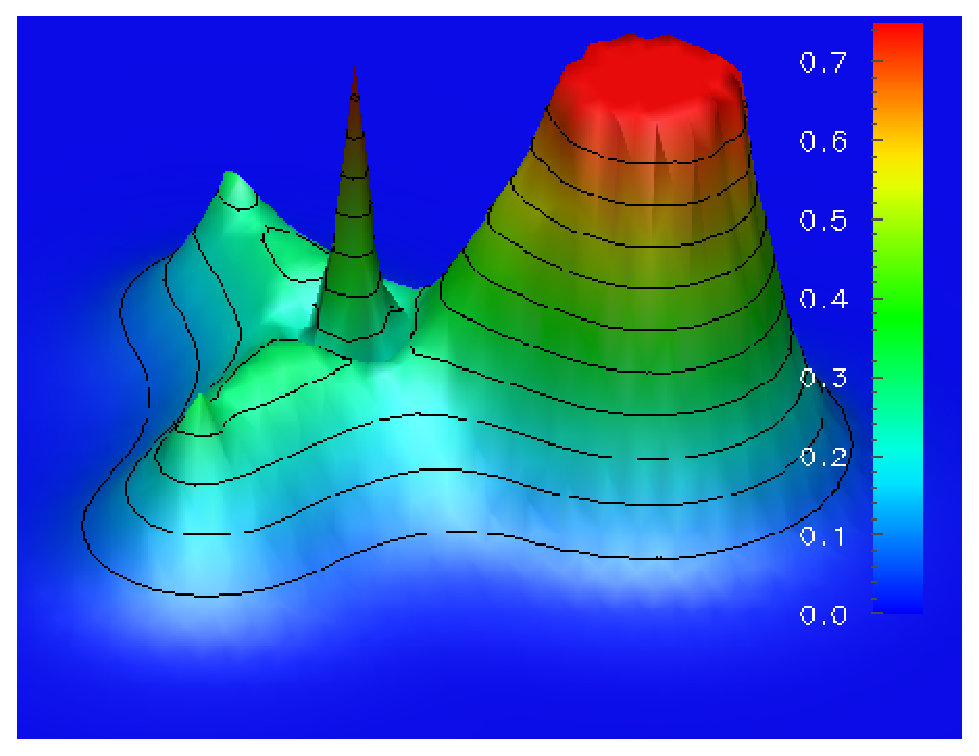
\includegraphics{Figs/h2co-rho.eps}}

  If your viewing direction is straight onto the plane, you will obtain
  a (color) contour plot.

  By adjusting the maximum value, you can cut off very large values,
  and thus obtain more detail for the lower density values.
\end{itemize}
\end{enumerate}

%==========================================================================
\subsection{View data using FreeWRL}
%==========================================================================
The wave tool constructs a scene in the virtual Reality Modeling
Language (VRML) format. The standard extension is ``.wrl''. A common
viewer is FreeWRL.

VRML has been superceeded by the language X3D. The syntax is very
similar and VRML files can be converted into X3D files.

%==========================================================================
\newpage
\subsection{Contour plots using Gnuplot}
%==========================================================================
If a plane has been specified in !WCNTL a input file for gnuplot to
produce contour plots is generated. It has the File id. 'GNUCONTOUR'
and the default file name \textit{rootname}\_c.gnu.

A plot is generated by the command
\begin{center}
\begin{minipage}{0.7\linewidth}
{\tt gnuplot {\it rootname}\_c.gnu $>$ tmp.eps}\\
{\tt gv tmp.eps}
\end{minipage}
\end{center}

The resulting file will look like
\begin{center}
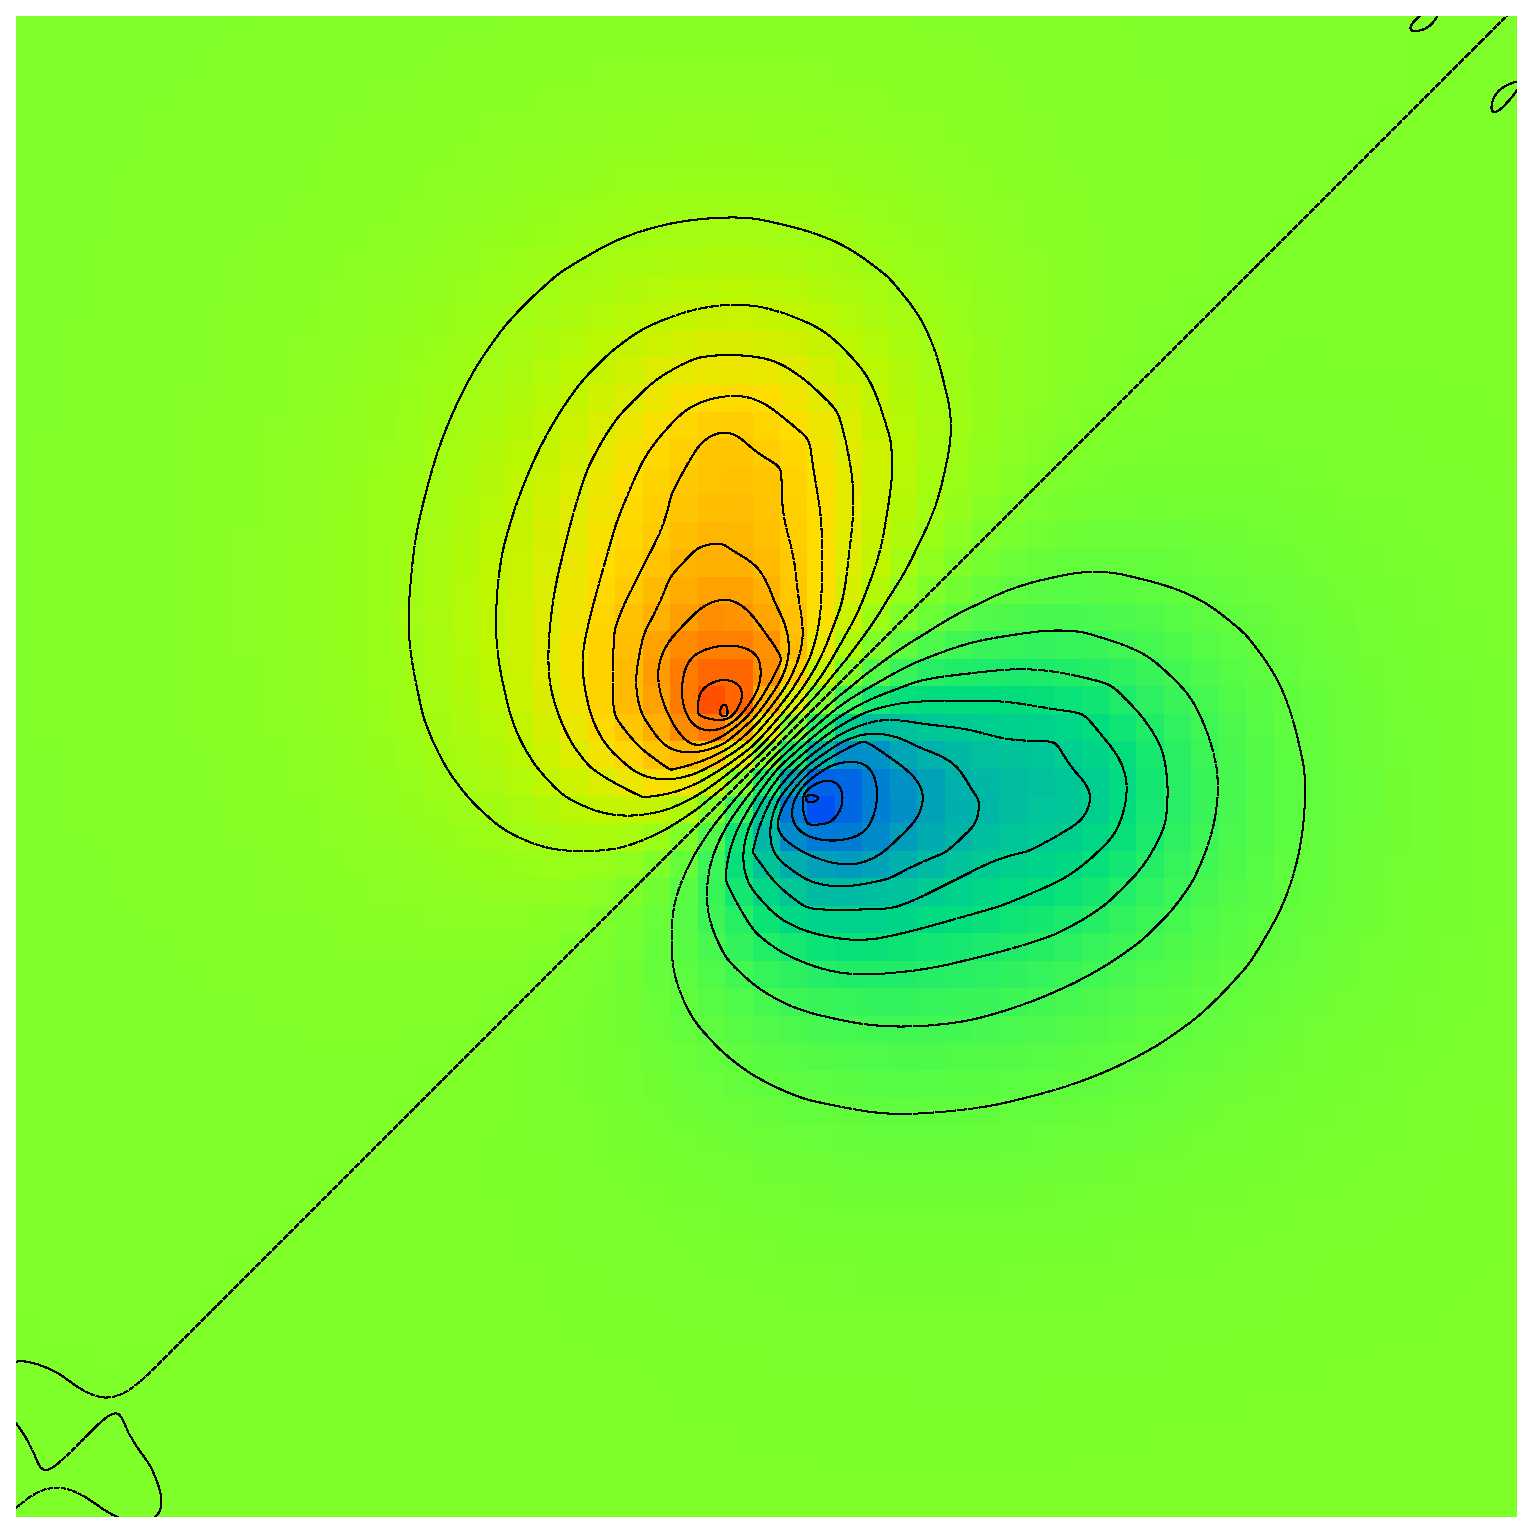
\includegraphics[width=0.5\linewidth,clip=true]{Figs/gnucontour.eps}
\end{center}


This plot may not be what one wants. You can edit the gnuplot
file. The top part looks something like the following: 
{\tiny\begin{verbatim}
#
 #==========================================================
 # DATA SECTION TO BE CHANGED BY THE USER                 ==
 #==========================================================
 xmin=  -5.0000000000000000     
 xmax=   5.0000000000000000     
 ymin=  -5.0000000000000000     
 ymax=   5.0000000000000000     
 zmin= -0.52367716662429253     
 zmax=  0.52367704490151912     
 rot_x=0
 rot_z=0
 scale=   2.0000000000000000     
 scale_z=1.
 #
 #==========================================================
 # DEFINE LINE STYLES TO BE USED WITH LS IN SPLOT         ==
 #==========================================================
 # DEFINE A LINESTYLE FOR SPLOT (USED WITH LS)
 set style line 1 lt 1 lc rgb "black" lw 1
 # MAP HIGHT VALUES TO COLORS
 set palette rgbformula 22,13,-31
 #
 #==========================================================
 # DATA RELATED STATEMENTS                                ==
 #==========================================================
 set xrange [xmin:xmax]
 set yrange [ymin:ymax]
 set zrange [zmin:zmax]
 set dgrid3d  60,60,1     #SAMPLE DATA ONTO A 60X60 GRID
 #
 #==========================================================
 # SURFACE PLOT                                           ==
 #==========================================================
 set surface
 set hidden3d
 set xyplane at 0.      # PLACE Z=0 INTO THE XY PLANE
 unset border           # REMOVE AXES
 unset xtics            # REMOVE TICS FROM THE AXES
 unset ytics            # REMOVE TICS FROM THE AXES
 unset ztics            # REMOVE TICS FROM THE AXES
 set key off            # REMOVE TITLE
 set pm3d hidden3d 0  # LINESTYLE FOR THE SURFACE GRID
 #
 #==========================================================
 # DEFINE CONTOUR                                         ==
 #==========================================================
 set contour surface # DRAW CONTOUR ONTO THE SURFACE
 set cntrparam levels incremental -0.5,0.05,0.5
 set cntrparam bspline
 set cntrparam order 6
 unset clabel # NO AUTOCOLORING OF CONTOURS
 #
 #==========================================================
 # DEFINE ORIENTATION                                     ==
 #==========================================================
 set view equal xy # avoids distortions of xy-plane
 #  ANGLE, ANGLE, OVERALL SCALE, SCALE Z-AXIS
 set view rot_x,rot_z,scale,scale_z
 #
 #==========================================================
 # SET Terminals (uncomment one)                          ==
 #==========================================================
 #----USE POSTSCRIPT TERMINAL FOR EPS FILES-----------------
 set terminal postscript eps size xmax-xmin,ymax-ymin  enhanced color clip font 'helvetica,20' linewidth 2 
 #----USE WXT TERMINAL FOR LINUX SCREEN---------------------
 # set terminal wxt size 350,262 enhanced  font 'verdana,10' persist 
 #----USE PDF TERMINAL FOR PDF FILES------------------------
 # set terminal pdf color enhanced 
 #----USE AQUA TERMINAL FOR OSX SCREEN----------------------
 # set terminal aqua enhanced solid font 'helvetica,20'title 'contour'
 #
 #==========================================================
 # PERFORM PLOT                                           ==
 #==========================================================
 # unset contour
 set border
 # unset surface
 unset colorbox
 splot '-' with pm3d linewidth 1 linecolor rgb '#000000'
 #
 #==========================================================
 # DATA SECTION                                           ==
 #==========================================================
  -5.0000000000000000       -5.0000000000000000       -6.3559036829332985E-009
  -5.0000000000000000       -4.8305084742605686        2.7132751008533330E-005
  -5.0000000000000000       -4.6610169485211372        8.1098647806454938E-005
  -5.0000000000000000       -4.4915254414081573        1.2624831976719569E-004
  -5.0000000000000000       -4.3220338970422745        1.1350877204762644E-004
  -5.0000000000000000       -4.1525423526763916        1.0682727783892541E-004
 \end{verbatim}}

\begin{enumerate}
\item adjust the parameters \verb|xmin|, \verb|xmax|, \verb|ymin|,
 \verb|ymax| to select the viewing area.
\item adjust the values in
 \verb|set cntrparam levels incremental -0.5,0.05,0.5| to select the
 values of the contours. The values are minimum value, increment,
 maximum value
\item if you do not like the coloring, uncomment the line 'unset surface'
\item select the terminal type to create a certain file type.
\end{enumerate}
%==========================================================================
\newpage
\subsection{Rubbersheets  using Gnuplot}
%==========================================================================
If a plane has been sepcified in !WCNTL a input file for gnuplot to
PRODUCE COUNTOUR PLOTS IS GENERATED. IT HAS THE FILE ID 'GNURUBBERSHEET'
and the default file name \textit{rootname}\_r.gnu.

A plot is generated by the command
\begin{center}
\begin{minipage}{0.7\linewidth}
{\tt gnuplot {\it rootname}\_r.gnu $>$ tmp.eps}\\
{\tt gv tmp.eps}
\end{minipage}
\end{center}

The resulting file will look like
\begin{center}
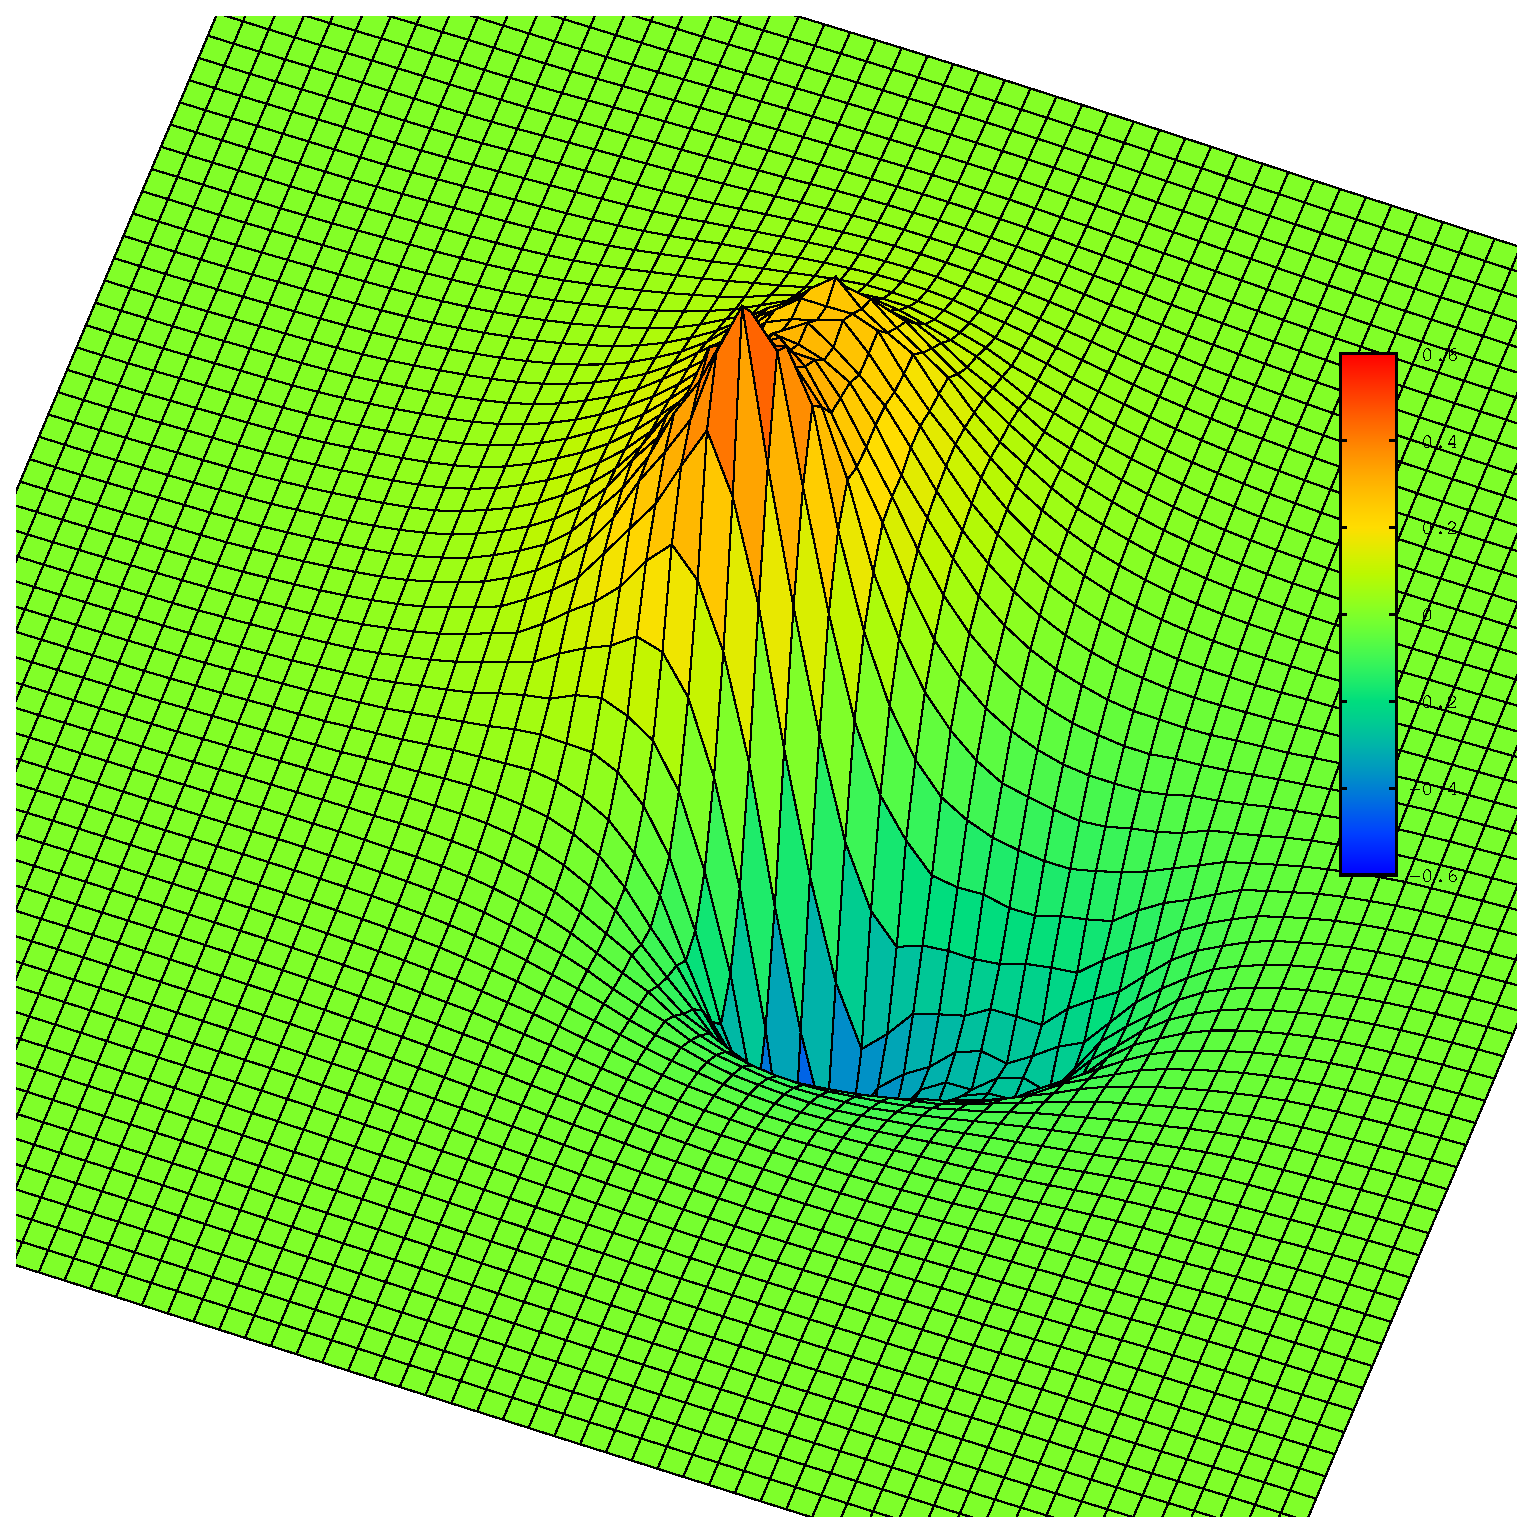
\includegraphics[width=0.5\linewidth,clip=true]{Figs/gnurubbersheet.eps}
\end{center}


This plot may not be what one wants. You can edit the gnuplot
file. The top part looks something like the following: 
{\tiny\begin{verbatim}
 #
 #==========================================================
 # DATA SECTION TO BE CHANGED BY THE USER                 ==
 #==========================================================
 xmin=  -5.0000000000000000     
 xmax=   5.0000000000000000     
 ymin=  -5.0000000000000000     
 ymax=   5.0000000000000000     
 zmin= -0.52367716662429253     
 zmax=  0.52367704490151912     
 rot_x=30
 rot_z=20
 scale=   2.0000000000000000     
 scale_z=1.
 #
 #==========================================================
 # DEFINE LINE STYLES TO BE USED WITH LS IN SPLOT         ==
 #==========================================================
 # DEFINE A LINESTYLE FOR SPLOT (USED WITH LS)
 set style line 1 lt 1 lc rgb "black" lw 1
 # MAP HIGHT VALUES TO COLORS
 set palette rgbformula 22,13,-31
 #
 #==========================================================
 # DATA RELATED STATEMENTS                                ==
 #==========================================================
 set xrange [xmin:xmax]
 set yrange [ymin:ymax]
 set zrange [zmin:zmax]
 set dgrid3d  60,60,1     #SAMPLE DATA ONTO A 60X60 GRID
 #
 #==========================================================
 # SURFACE PLOT                                           ==
 #==========================================================
 set surface
 set hidden3d
 set xyplane at 0.      # PLACE Z=0 INTO THE XY PLANE
 unset border           # REMOVE AXES
 unset xtics            # REMOVE TICS FROM THE AXES
 unset ytics            # REMOVE TICS FROM THE AXES
 unset ztics            # REMOVE TICS FROM THE AXES
 set key off            # REMOVE TITLE
 set pm3d hidden3d 1  # LINESTYLE FOR THE SURFACE GRID
 #
 #==========================================================
 # DEFINE CONTOUR                                         ==
 #==========================================================
 set contour surface # DRAW CONTOUR ONTO THE SURFACE
 set cntrparam levels incremental -0.5,0.05,0.5
 set cntrparam bspline
 set cntrparam order 6
 unset clabel # NO AUTOCOLORING OF CONTOURS
 #
 #==========================================================
 # DEFINE ORIENTATION                                     ==
 #==========================================================
 set view equal xy # avoids distortions of xy-plane
 #  ANGLE, ANGLE, OVERALL SCALE, SCALE Z-AXIS
 set view rot_x,rot_z,scale,scale_z
 #
 #==========================================================
 # SET Terminals (uncomment one)                          ==
 #==========================================================
 #----USE POSTSCRIPT TERMINAL FOR EPS FILES-----------------
 set terminal postscript eps size xmax-xmin,ymax-ymin  enhanced color clip font 'helvetica,20' linewidth 2 
 #----USE WXT TERMINAL FOR LINUX SCREEN---------------------
 # set terminal wxt size 350,262 enhanced  font 'verdana,10' persist 
 #----USE PDF TERMINAL FOR PDF FILES------------------------
 # set terminal pdf color enhanced 
 #----USE AQUA TERMINAL FOR OSX SCREEN----------------------
 # set terminal aqua enhanced solid font 'helvetica,20'title 'contour'
 #
 #==========================================================
 # PERFORM PLOT                                           ==
 #==========================================================
 unset contour
 # set border
 # unset surface
 # unset colorbox
 splot '-' with pm3d linewidth 1 linecolor rgb '#000000'
 #
 #==========================================================
 # DATA SECTION                                           ==
 #==========================================================
  -5.0000000000000000       -5.0000000000000000       -6.3559036829332985E-009
  -5.0000000000000000       -4.8305084742605686        2.7132751008533330E-005
  -5.0000000000000000       -4.6610169485211372        8.1098647806454938E-005
  -5.0000000000000000       -4.4915254414081573        1.2624831976719569E-004
\end{verbatim}}

\begin{enumerate}
\item adjust orientation by changing the parameters \verb|rot_x| and
  \verb|rot_z|
\item adjust the viewing area by changing the parameters \verb|xmin|,
  \verb|xmax|, \verb|ymin|, \verb|ymax|
\item if you like contours on the surface, comment the line 'unset surface'
\item select the terminal type to create a certain file type.
\end{enumerate}



%==========================================================================
\newpage
\section{Wave function converter for CryMolCAD: ``paw\_cmcwave''}
%==========================================================================
The tool converts the wave function file .wv produced by the
simulaation code into an input file for the CrymolCAD viewer. The wave
function can be a general field such as wave function, density or
potential.
\begin{center}
paw\_cmcwave.x case.wv
\end{center}
A new file is case.cmcv created, which can be read by CryMolCAD. The
file contains only the information for the field. The structure
information must be supplied separately.


%==========================================================================
\newpage
\section{Band-Offset and Work-Function Tool: ``paw\_1davpot''}
%==========================================================================
The tool ``paw\_1davpot'' produces the one dimensional potential
obtained by averaging the potential over lattice planes. By comparing
with the respective bulk calculations one can determine the band
offsets or work functions.

The tool uses the electrostatic potential produced by the CP-PAW code
using the option !control!analyse!potential. If the file of the
resulting potential file is ``case\_pot.wv'',  the calling sequence is
\begin{center}
paw\_1davpot.x case\_pot.wv
\end{center}
Three files are produced, namely AVPOT100.DAT, AVPOT010.DAT and
AVPOT001.DAT. The first is an xy file of the averaged potential along
the normal of the plane spanned by the lattice vectors $\vec{T}_2$ and
$\vec{T}_3$. The other files contain the corresponding information
along the two other plane normals.

In order to obtain a band offset from a supercell calculation
determine first the one-dimensional potential $v_{sup}(z)$ averaged
over planes parallel to the surface or interface. Next perform a
calculation of the bulk material using exactly the same geometry
(including any lateral strain), and determine the averaged potentials
$v_{bulk A}(z)$ and $v_{bulk,B}$ for the same lattice planes.
Determine furthermore the Fermi-level or the valence band top in the bulk
materials $e_{vbt,A}$ and $e_{vbt,B}$.

By forming the corresponding differences, one obtains a spatially
dependent valence band top $e'_{vbt,A}$ and $e'_{vbt,B}$ 
for the slab calculation.
\begin{eqnarray*}
e'_{vbt,A}(z)=e_{vbt,A}-v_{bulk,A}(z+\Delta z_A)+v_{sup}(z)
\\
e'_{vbt,B}(z)=e_{vbt,B}-v_{bulk,A}(z+\Delta z_B)+v_{sup}(z)
\end{eqnarray*}
The shift $\Delta z_{A/B}$ are needed to account for the difference in
z-coordinates for the lattice planes in the bulk and in the supercell.

If the spatially dependent valence band tops converge to a constant
value in the interior of the slab, this value can be taken as the
position of the valence band top in the supercell.
 

%==========================================================================
\newpage
\section{The Trajectory Analysis Tool: ``paw\_tra''}
%==========================================================================
This trajectory analysis tool is used to inspect atomic trajectories. It
allows one to create a movie input file for OPENDX\cite{opendx}, or print the
time evolution of selected bond lengths, angles, torsions or any combination
thereof.

The time scale is measured in psec. (If you cannot view the ball stick
model in OPENDX\cite{opendx}, please convert the dx file globally to
lower case.)

%==========================================================================
\subsection{Command}
%==========================================================================
The calling sequence is

\bigskip\fbox{{\tt paw\_tra} {\it controlfile}}\bigskip

\noindent
where {\it controlfile} is the file name of the control input file for
the paw\_tra tool. I recommend the extension
``.tcntl''.

%==========================================================================
\subsection{Example for the control input file}
%==========================================================================
\begin{verbatim}
!TCNTL
  !FILES
    !FILE ID='STRC' 
          NAME='~/PAW/Sample/h2co.strc_out' !END
    !FILE ID='TRA' 
          NAME='~/PAW/Sample/h2co_r.tra' !END
  !END
  !SEQUENCE T1[PS]=0. T2[PS]=2. DT[FS]=1. !END
  !MOVIE skip=2
    !VIEWBOX O=3*-5.  T=10. 3*0. 10. 3*0. 10. !END
    !FILE  EXT=T NAME='_movie.dx' !END
  !END
  !temperature retard[ps]=0.1
    !select atoms= 'H_1' 'H_2' !END
    !FILE  EXT=T NAME='.h.temp.dx' !END
  !end  
  !spaghetti
    !FILE  EXT=T NAME='.temp.pasta' !END
  !end  
  !MODE ID='H-C-BOND' 
    !BOND SCALE=1.0 ATOM1='H_1' ATOM2='C_3' !END
  !END 
  !MODE ID='H-ANTI-STRETCH' 
    !MODE SCALE=1.0 ID='H1-C-BOND' !END
    !BOND SCALE=-1.0 ATOM1='H_2' ATOM2='C_3' !END
  !END 
  !MODE ID='H-C-H-ANGLE' 
    !ANGLE SCALE=1.0 ATOM1='H_1' ATOM2='C_3' 
           ATOM3='H_2' !END
  !END 
  !OUTPUT ID='H-ANTI-STRETCH' TYPE='VELOCITY' !END
!END
!EOB
\end{verbatim}

%==========================================================================
\subsection{Argument description for the control input file ``tcntl''}
%==========================================================================


%----------------------------------------------------------------------
\block{!TCNTL}
%----------------------------------------------------------------------
\brules{mandatory}
\bdescr{}


%----------------------------------------------------------------------
\block{!TCNTL!FILES}
%----------------------------------------------------------------------
\brules{optional}
\bdescr{specifies the file names that deviate from standard file names}

\mbax{\key{ROOT}
\vdescr{root name. Files defined as extension will have this name
  combined with the extension. All files connected as default are
  defined as extensions.}
\vformat{character}
\vrules{optional}
\vdefault{string preceding the '.tcntl' ending of the control input file}}

%----------------------------------------------------------------------
\block{!TCNTL!FILES!FILE}
%----------------------------------------------------------------------
\brules{optional, multiple}
\bdescr{define the file name:
\begin{itemize}
\item {\bf PROT} protocol. Standard extension: '.tprot'
\item {\bf CNTL} control input file for the paw\_tra tool. The name of
  this file is mandatory input and cannot be reset.
\item {\bf STRC} structure output file produced by the
  simulation and used as input. standard extension: '.strc\_out'
\item {\bf TRA} trajectory file produced by the
  simulation and used as input. standard extension: '\_r.tra'
\end{itemize}
}

\mbax{\key{ID}
\vdescr{Identifier of the file.}
\vformat{character} 
\vrules{mandatory}
\vdefault{none}}

\mbax{\key{EXT}
\vdescr{rootname flag: if true, the filename is interpreted as an
  extension of the rootname. The rootname is the filename of the
  wavecontrol file without the last dot and the following characters.}
\vformat{logical} 
\vrules{optional}
\vdefault{.false.}}

\mbax{\key{NAME}
\vdescr{File name}
\vformat{character} 
\vrules{mandatory}
\vdefault{none}}

%----------------------------------------------------------------------
\block{!TCNTL!SEQUENCE}
%----------------------------------------------------------------------
\brules{optional} 
\bdescr{specifies the beginning and ending time and the sampling
  frequency of the sequence to be analyzed.}

\mbax{\key{T1[PS]}
\vdescr{Beginning time of the sequence in picoseconds}
\vformat{real} 
\vrules{optional}
\vdefault{time of the first frame on the trajectory file}}

\mbax{\key{T2[PS]}
\vdescr{ending time of the sequence in picoseconds}
\vformat{real} 
\vrules{optional}
\vdefault{time of the last frame on the trajectory file}}

\mbax{\key{DT[FS]}
\vdescr{sampling frequency in femtoseconds}
\vformat{real} 
\vrules{optional}
\vdefault{spacing on the trajectory file}}

%----------------------------------------------------------------------
\block{!TCNTL!MOVIE}
%----------------------------------------------------------------------
\brules{optional} 
\bdescr{writes a input file for OPENDX\cite{opendx} to show the moving atoms as a
  ball-stick model. Bonds are drawn for every pair of atoms that are
  closer than 1.2 times the sum of the covalent radii.}

\mbax{\key{FORMAT}
\vdescr{descriptor for the format of the movie file to be created. can
  be 'DX' (OPENDX\cite{opendx}), 'XYZ' (xyz format)}
\vformat{character} 
\vrules{optional}
\vdefault{'DX'}}

\mbax{\key{SKIP}
\vdescr{number of frames on the input trajectory files that are
  skipped between movie frames}
\vformat{integer} 
\vrules{optional}
\vdefault{0.}}


%----------------------------------------------------------------------
\block{!TCNTL!MOVIE!VIEWBOX}
%----------------------------------------------------------------------
\brules{optional} 
\bdescr{Sets the view box. Only the data within the
  view box are shown. The view box is defined by an origin $o$ and three
  vectors $t_1,t_2,t_3$. The eight corners of the view box are
  $o,o+t_1,o+t_2,o+t_3,o+t_1+t_2,o+t_2+t_3,o+t_1+t_3,o+t_1+t_2+t_3$}

\mbax{\key{O}
\vdescr{Origin (lower left, forward point of the view box) in a.u.}
\vformat{real} 
\vrules{optional; incompatible with ``!TCNTL!MOVIE!VIEWBOX:C''}
\vdefault{0. 0. 0.}}

\mbax{\key{C}
\vdescr{Center of viewbox}
\vformat{real} 
\vrules{optional; incompatible with ``!TCNTL!MOVIE!VIEWBOX:O''}
\vdefault{see ``!TCNTL!MOVIE!VIEWBOX:O''}}

\mbax{\key{T}
\vdescr{vectors defining the edges of the view box}
\vformat{real(3,3)} 
\vrules{optional}
\vdefault{lattice vectors of the calculation}}

%----------------------------------------------------------------------
\block{!TCNTL!MOVIE!FILE}
%----------------------------------------------------------------------
\brules{optional} 
\bdescr{specify the file where the movie plot is written. The file
  is then used with an appropriate visualizer.}
\mbax{\key{EXT}
\vdescr{switch to the rootname appended by the extension provided,
  versus using the filename (including its path).}
\vformat{logical} 
\vrules{optional}
\vdefault{.false.}}

\mbax{\key{NAME}
\vdescr{file name}
\vformat{character} 
\vrules{optional}
\vdefault{the rootname appended by ``.movie.dx'' for 
!TCNTL!MOVIE:FORMAT='DX' and by ``.movie.xyz'' for 
!TCNTL!MOVIE:FORMAT='XYZ'}}

%----------------------------------------------------------------------
\block{!TCNTL!MOVIE!SELECT}
%----------------------------------------------------------------------
\brules{optional} 
\bdescr{specify the atoms to shall be used. Unless specified, all
  atoms are plotted.}

\mbax{\key{ATOMS}
\vdescr{atom names consistent with the ``strc'' file. An arbitrary
  number of atoms can be included}
\vformat{character} 
\vrules{mandatory}
\vdefault{none}}

%----------------------------------------------------------------------
\block{!TCNTL!CORRELATION}
%----------------------------------------------------------------------
\brules{optional} 
\bdescr{evaluates pair correlation functions
\begin{eqnarray}
g_{C,P}(d)=\frac{1}{T_2-T_1}\int_{T_1}^{T_2}dt\;
\frac{1}{N_C}\sum_{i\in C}\sum_{j\in P}
\delta\left(\left|R_j(t)-\vec{R}_i(t)\right|-d\right)
\nonumber
\end{eqnarray}
where $[T_1,T_2]$ is the selected time interval. $C$ is the set of
center atoms selectrd in \texttt{!TCNTL!CORRELATION!CENTER} and $P$ is
the set of partner atoms selected in
\texttt{!TCNTL!CORRELATION!PARTNER}.

The histogram is currently plotted up to a maximum distance of
$d_x=5$~\AA. The histogram is a density on the distance grid, which is
normalized by the number of center atoms.

Warning! Currently the code selects a set of atom pairs from the
initial time slice in the specified time interval and monitors the
distances of only these pairs. Atom pairs with initial distances above
$2\times d_x$~\AA (i.e. 10~\AA) are ignored.}

%% \mbax{\key{TYPE}
%% \vdescr{select distance or angle correlation. (Angle correlations not
%%   yet implemented!)}
%% \vformat{character(1); allowed values are 'D' for distance and 'A' for
%%   angle} 
%% \vrules{optional}
%% \vdefault{'D'}}

%% \mbax{\key{DEP}
%% \vdescr{selects correlation over time as spaghetti plot or the time
%%   averaged histogram as function of angle or distance.}
%% \vformat{character; allowed values are 'SPAGHETTI' and 'HISTOGRAM'} 
%% \vrules{optional}
%% \vdefault{'HISTOGRAM'}}

%----------------------------------------------------------------------
\block{!TCNTL!CORRELATION!FILE}
%----------------------------------------------------------------------
\brules{optional} 
\bdescr{specify the file where output (histogram or spaghetti) is written to.}

\mbax{\key{EXT}
\vdescr{switch to the rootname appended by the extension provided,
  versus using the filename (including its path).}
\vformat{logical} 
\vrules{optional}
\vdefault{.false.}}

\mbax{\key{NAME}
\vdescr{file name}
\vformat{character} 
\vrules{optional}
\vdefault{the rootname appended by ``.tra.correlation''}}

%----------------------------------------------------------------------
\block{!TCNTL!CORRELATION!CENTER}
%----------------------------------------------------------------------
\brules{optional} 
\bdescr{specify the atoms to be used. Unless specified, all
  atoms are plotted.}
%----------------------------------------------------------------------
\block{!TCNTL!CORRELATION!CENTER!SELECT}
%----------------------------------------------------------------------
\brules{optional} 
\bdescr{specify the atoms to be used, as reference atoms. Unless specified, all
  atoms are SELECTED.}

\mbax{\key{ATOMS}
\vdescr{atom names consistent with the ``strc'' file. An arbitrary
  number of atoms can be included}
\vformat{character} 
\vrules{mandatory}
\vdefault{none}}

%----------------------------------------------------------------------
\block{!TCNTL!CORRELATION!PARTNER}
%----------------------------------------------------------------------
\brules{optional} \bdescr{specify the atoms to be used as partner
  atoms. Unless specified, all atoms are selected.}

%----------------------------------------------------------------------
\block{!TCNTL!CORRELATION!PARTNER!SELECT}
%----------------------------------------------------------------------
\brules{optional} 
\bdescr{specify the atoms to be used. Unless specified, all
  atoms are selected.}

\mbax{\key{ATOMS}
\vdescr{atom names consistent with the ``strc'' file. An arbitrary
  number of atoms can be included}
\vformat{character} 
\vrules{mandatory}
\vdefault{none}}

%----------------------------------------------------------------------
\block{!TCNTL!SNAPSHOT}
%----------------------------------------------------------------------
\brules{optional} 
\bdescr{picks the unit cell and the atomic position for a given
  snapshot in a trajectory. The data are written to the protocoll file
  in a pseudo format for the structure input file and as cssr file to
  the file specified.}

\mbax{\key{T[PSEC]}
\vdescr{time at which the snapshot shall be taken out of the
  trajectory. The code selects the last timestep before the given time.}
\vformat{real} 
\vrules{either T[PSEC] or STEP must be selected}
\vdefault{none}}

\mbax{\key{STEP}
\vdescr{time step number at which the snapshot shall be taken out of the
  trajectory.}
\vformat{integer} 
\vrules{either T[PSEC] or STEP must be selected}
\vdefault{none}}

%----------------------------------------------------------------------
\block{!TCNTL!SNAPSHOT!FILE}
%----------------------------------------------------------------------
\brules{optional} 
\bdescr{specify the file where cssr file is written to.}

\mbax{\key{EXT}
\vdescr{switch to the rootname appended by the extension provided,
  versus using the filename (including its path).}
\vformat{logical} 
\vrules{optional}
\vdefault{.false.}}

\mbax{\key{NAME}
\vdescr{file name}
\vformat{character} 
\vrules{optional}
\vdefault{the rootname appended by ``.tra.cssr''}}

%% %----------------------------------------------------------------------
%% \block{!TCNTL!SPAGHETTI!SELECT}
%% %----------------------------------------------------------------------
%% \brules{optional} 
%% \bdescr{specify the atoms to be used. Unless specified, all
%%   atoms are plotted.}

%% \mbax{\key{ATOMS}
%% \vdescr{atom names consistent with the ``strc'' file. An arbitrary
%%   number of atoms can be included}
%% \vformat{character} 
%% \vrules{mandatory}
%% \vdefault{none}}

%----------------------------------------------------------------------
\block{!TCNTL!CELL}
%----------------------------------------------------------------------
\brules{optional}
\bdescr{write unit cell to file as function of time}

\mbax{\key{TIMEFORMAT}}
\vdescr{switch to usage of time in picosecond instead of the 
number of iteration}
\vformat{logical}
\vrules{optional}
\vdefault{.false.}

%----------------------------------------------------------------------
\block{!TCNTL!CELL!FILE}
%----------------------------------------------------------------------
\brules{optional} 
\bdescr{specify the file where cell data  is written to}

\mbax{\key{EXT}
	\vdescr{switch to the rootname appended by the extension provided,
		versus using the filename (including its path).}
	\vformat{logical} 
	\vrules{optional}
	\vdefault{F}}

\mbax{\key{NAME}
	\vdescr{file name}
	\vformat{character} 
	\vrules{optional}
	\vdefault{the rootname appended by ``.tra.cell''}}

%----------------------------------------------------------------------
\block{!TCNTL!SPAGHETTI}
%----------------------------------------------------------------------
\brules{optional} 
\bdescr{performs a spaghetti plot ($|R(t)-R(0)|$) for a number of atoms}

%----------------------------------------------------------------------
\block{!TCNTL!SPAGHETTI!FILE}
%----------------------------------------------------------------------
\brules{mandatory} 
\bdescr{specify the file where the spaghetti plot is written. The file
  is formatted and to be used with an x-y plotting tool. Each line
  contains the time in ps and the distance in Angstrom}

\mbax{\key{EXT}
\vdescr{switch to the rootname appended by the extension provided,
  versus using the filename (including its path).}
\vformat{logical} 
\vrules{optional}
\vdefault{.false.}}

\mbax{\key{NAME}
\vdescr{file name}
\vformat{character} 
\vrules{optional}
\vdefault{the rootname appended by ``.tra.pasta''}}

%----------------------------------------------------------------------
\block{!TCNTL!SPAGHETTI!SELECT}
%----------------------------------------------------------------------
\brules{optional} 
\bdescr{specify the atoms to be used. Unless specified, all
  atoms are plotted.}

\mbax{\key{ATOMS}
\vdescr{atom names consistent with the ``strc'' file. An arbitrary
  number of atoms can be included}
\vformat{character} 
\vrules{mandatory}
\vdefault{none}}

%----------------------------------------------------------------------
\block{!TCNTL!TEMPERATURE}
%----------------------------------------------------------------------
\brules{optional, multiple} \bdescr{prints the average temperatures of
  the atoms and optionally a plot for the temperature versus time for
  individual atoms.  \textbf{Warning:} The temperatures are obtained
  from the kinetic energy using $g=3N$ where $N$ is the number of
  atoms in the selected group. If translations and/or rotations are
  excluded, the temperature given here is underestimated and must be
  rescaled by a factor $3N/(3N-5)$ for dimers, $3N/(3N-6)$ for other
  molecules, $3N/(3N-3)$ for solids.}

\mbax{\key{RETARD[PS]}
\vdescr{The values are averaged over previous values with exponential
  decay. 
  $$x(t)=\frac{1}{t_0}\int_{-\infty}^{t} dt^\prime 
  x(t^\prime) \exp(-\frac{t-t^\prime}{t_0})$$
  This value is the decay time $t_0$ in pico seconds.}
\vformat{real} 
\vrules{optional}
\vdefault{0.}}

%----------------------------------------------------------------------
\block{!TCNTL!TEMPERATURE!SELECT}
%----------------------------------------------------------------------
\brules{optional} 
\bdescr{specify the atoms to be used. Unless specified, all
  atoms are plotted.}

\mbax{\key{ATOMS}
\vdescr{atom names consistent with the ``strc'' file. An arbitrary
  number of atoms can be included}
\vformat{character} 
\vrules{mandatory}
\vdefault{none}}

%----------------------------------------------------------------------
\block{!TCNTL!TEMPERATURE!FILE}
%----------------------------------------------------------------------
\brules{mandatory} 
\bdescr{specifies the file where the  plot is written. The file
  is formatted and to be used with an x-y plotting tool. Each line
  containes the time in ps and the temperature in Kelvin}

\mbax{\key{EXT}
\vdescr{switch to the rootname appended by the extension provided,
  versus using the filename (including its path).}
\vformat{logical} 
\vrules{optional}
\vdefault{.false.}}

\mbax{\key{NAME}
\vdescr{file name}
\vformat{character} 
\vrules{optional}
\vdefault{the rootname appended by ``.tra.temp''}}
%
%----------------------------------------------------------------------
\block{!TCNTL!SOFT}
%----------------------------------------------------------------------
\brules{optional} 
\bdescr{produces the mass weighted path-length versus time 
  $$s(t)=\int_0^t \sqrt{\sum_i M_i\dot{R}_i^2}$$.  This mapping can be
  used to transform a time scale to a length scale, using the
  definitions of the intrinsic reaction coordinate
  (IRC)\cite{fukui70_jcp74_4161,fukui81_acr14_363}.  The unit of the
  mass weighted path length is \AA$\sqrt{{\rm u}}$, where u is the
  ``atomic mass unit'', i.e. one twelfth of the mass of $^{12}$C.}
%
%----------------------------------------------------------------------
\block{!TCNTL!SOFT!SELECT}
%----------------------------------------------------------------------
\brules{optional} 
\bdescr{specify the atoms to be used. Unless specified, all
  atoms are used.}
%
\mbax{\key{ATOMS}
\vdescr{atom names consistent with the ``strc'' file. An arbitrary
  number of atoms can be included}
\vformat{character} 
\vrules{mandatory}
\vdefault{none}}
%
%----------------------------------------------------------------------
\block{!TCNTL!SOFT!FILE}
%----------------------------------------------------------------------
\brules{optional} 
\bdescr{specify the file where the mass-weighted path length versus time is written. The file
  is formatted and to be used with an x-y plotting tool. Each line
  contains the time in ps and the distance in angstrom}

\mbax{\key{EXT}
\vdescr{switch to the rootname appended by the extension provided,
  versus using the filename (including its path).}
\vformat{logical} 
\vrules{optional}
\vdefault{.false.}}

\mbax{\key{NAME}
\vdescr{file name}
\vformat{character} 
\vrules{optional}
\vdefault{the rootname appended by ``.tra.soft''}}


%----------------------------------------------------------------------
\block{!TCNTL!NEIGHBORS}
%----------------------------------------------------------------------
\brules{optional} 
\bdescr{print a neighborlist at the beginning and the end of a
  trajectory and report all bon-breaking and bond-forming events. The
  report will be written into a file with extension ``.tra.neighbors''}

%----------------------------------------------------------------------
\block{!TCNTL!MODE}
%----------------------------------------------------------------------
\brules{optional} \bdescr{defines a vibrational mode of the system
  such as a bond length, an angle etc. Note that all bond vectors that
  define bonds, angles or torsions are mapped onto the minimum image.}

\mbax{\key{ID}
\vdescr{Identifier of this mode to be used in further operations can
  be any string, but different from all other mode-identifiers.}
\vformat{character} 
\vrules{mandatory}
\vdefault{none}}

%----------------------------------------------------------------------
\block{!TCNTL!MODE!BOND}
%----------------------------------------------------------------------
\brules{optional} 
\bdescr{adds a bond length as a contribution defining a mode. The bond
  is defined as the distance between two atoms $R_1,R_2$.}

\mbax{\key{SCALE}
\vdescr{Scales the parameter before adding it to the mode. (Used for
  example to define symmetric and antisymmetric bond stretch modes.)}
\vformat{real} 
\vrules{mandatory}
\vdefault{none}}

\mbax{\key{ATOM1}
\vdescr{Name of the first atom $R_1$ defining the bond. The name is
  chosen  consistent with the structure input file of the simulation code.}
\vformat{character} 
\vrules{mandatory}
\vdefault{none}}

\mbax{\key{ATOM2}
\vdescr{Name of the second atom $R_2$ defining the bond. The name is
  chosen  consistent with the
  structure input file of the simulation code.}
\vformat{character} 
\vrules{mandatory}
\vdefault{none}}

%----------------------------------------------------------------------
\block{!TCNTL!MODE!ANGLE}
%----------------------------------------------------------------------
\brules{optional} 
\bdescr{adds a bond angle as a contribution defining a mode. The bond
  angle is the angle between the two bonds $(R_1,R_2)$ and $(R_2,R_3)$
The unit for angles is such that $2\pi$ is a full turn.}

\mbax{\key{SCALE}
\vdescr{Scales the parameter before adding it to the mode.}
\vformat{real} 
\vrules{mandatory}
\vdefault{none}}

\mbax{\key{ATOM1}
\vdescr{Name of the first terminal atom $R_1$ defining the bond
  angle. The name is chosen 
 consistent with the structure input file of the simulation code.}
\vformat{character} 
\vrules{mandatory}
\vdefault{none}}

\mbax{\key{ATOM2}
\vdescr{Name of the central atom $R_2$ defining the bond angle. The
  name is chosen consistent
  with the structure input file of the simulation code.}
\vformat{character} 
\vrules{mandatory}
\vdefault{none}}

\mbax{\key{ATOM3}
\vdescr{Name of the second terminal atom $R_3$ defining the bond
  angle. The name is chosen consistent
  with the structure input file of the simulation code.}
\vformat{character} 
\vrules{mandatory}
\vdefault{none}}

%----------------------------------------------------------------------
\block{!TCNTL!MODE!TORSION}
%----------------------------------------------------------------------
\brules{optional} 
\bdescr{
  Warning! this option does not seem to work!
  adds a bond torsion as a contribution defining a mode.  The
  unit for angles is such that $2\pi$ is a full turn. A torsion is
  defined by four atoms $(R_1,R_2,R_3,R_4)$. The torsion about the
  central bond $(R_2,R_3)$ is the angle between the two planes defined
  by two triples $(R_1,R_2,R_3)$ and $(R_2,R_3,R_4)$.}

\mbax{\key{SCALE}
\vdescr{Scales the parameter before adding it to the mode.}
\vformat{real} 
\vrules{mandatory}
\vdefault{none}}

\mbax{\key{ATOM1}
\vdescr{Name of the atom $R_1$ defining the bond torsion
 consistent with the structure input file of the simulation code.}
\vformat{character} 
\vrules{mandatory}
\vdefault{none}}

\mbax{\key{ATOM2}
\vdescr{Name of the atom $R_2$ defining the bond torsion consistent
  with the structure input file of the simulation code.}
\vformat{character} 
\vrules{mandatory}
\vdefault{none}}

\mbax{\key{ATOM3}
\vdescr{Name of the atom $R_3$ defining the bond torsion consistent
  with the structure input file of the simulation code.}
\vformat{character} 
\vrules{mandatory}
\vdefault{none}}

\mbax{\key{ATOM4}
\vdescr{Name of the  atom $R_4$ defining the bond torsion consistent
  with the structure input file of the simulation code.}
\vformat{character} 
\vrules{mandatory}
\vdefault{none}}

%----------------------------------------------------------------------
\block{!TCNTL!MODE!MODE}
%----------------------------------------------------------------------
\brules{optional} 
\bdescr{adds a predefined mode as a contribution defining a mode.}

\mbax{\key{SCALE}
\vdescr{Scales the parameter before adding it to the mode.}
\vformat{real} 
\vrules{mandatory}
\vdefault{none}}

\mbax{\key{ID}
\vdescr{ID of the mode to be included.}
\vformat{character} 
\vrules{mandatory}
\vdefault{none}}

%----------------------------------------------------------------------
\block{!TCNTL!OUTPUT}
%----------------------------------------------------------------------
\brules{optional, multiple} 
\bdescr{writes the time dependence of a mode to file}

\mbax{\key{ID}
\vdescr{identifier of the mode to be printed}
\vformat{character} 
\vrules{mandatory}
\vdefault{none}}

\mbax{\key{FILENAME}
\vdescr{file name of the file to which the result is written}
\vformat{character} 
\vrules{mandatory}
\vdefault{none}}

\mbax{\key{TYPE}
\vdescr{Defines the property to be written, 
\begin{itemize} 
\item default: the mode itself
\item '\texttt{VELOCITY}' the time derivative of the mode
\end{itemize}}
\vformat{character} 
\vrules{optional}
\vdefault{position}}

%==========================================================================
\subsection{View data using OPENDX\cite{opendx}}
%==========================================================================
Start the Dataexplorer using

\bigskip\fbox{{\tt dx -image \&}}\bigskip

\begin{enumerate}
\item Select ``{\bf Load Macro}'' from the ``{\bf File}'' pulldown
  menu. In the file selector, which pops up, check that you are in
  the DX subdirectory of the PAW directory and click on ``{\bf Load
    all macros}''.
\item Select ``{\bf Open}'' from the ``{\bf File}'' pulldown menu. In the file
  selector, which pops up, select the dx program ``{\bf tra.net}''.
\item select ``{\bf open all control panels}'' from the ``{\bf
    windows}'' pulldown menu.
\item In the ``{\bf Main Control Panel}'' that opens, select the input
  data file. You can do this by typing the file name into the text
  field of the file selector, or by pressing the button to the right of
  the text field and by maneuvering towards the right file in the
  file selector menu. After selecting the correct file, press OK.
\item Select ``{\bf Sequencer}'' from the ``{\bf Execute}'' Pulldown menu.
\item Use the sequencer like a VCR. (In the existing version, an error
  frequently occurs while reading the data file. The message says that it
  cannot read beyond a certain number of time slices. Remember the
  number, click on the right upper field of the sequencer, and type the
  number into the field for max. Then click on the same field of the
  sequencer, and continue.)
\end{enumerate}

%==========================================================================
\newpage
\section{The Density of States Analysis Tool: paw\_dos}
%==========================================================================
The paw\_dos tool allows one to analyze binding, both locally and energy
resolved. It can tell you which states contribute mostly to a
particular $\sigma, \pi, \delta$ bond. For example, you can learn whether
either bonding and antibonding states are close to the Fermi level
(HOMO-LUMO gap), in which case a structural deformation or a charge
transfer can affect such a bond strongly. This analysis is similar in
spirit to the Crystal-Orbital-Overlap-Population (COOP) analysis of R.
Hoffmann. It is of tremendous value to obtain a chemical (local)
description of binding in complex systems, where states are
delocalized and closely spaced in energy.

%==========================================================================
\subsection{Command}
%==========================================================================

The calling sequence is

\bigskip\fbox{{\tt paw\_dos} {\it controlfile}}\bigskip

\noindent
where {\it controlfile} is the file name of the control input file for
the paw\_dos tool. I recommend the extension ``.dcntl''.


%==========================================================================
\subsection{Theoretical basis for the paw\_dos tool}
%==========================================================================

The density of states matrix is defined as follows
\begin{equation}
  D_{\chi,\chi^\prime}(\epsilon)
 =\sum_n
  \langle\chi|\Psi_n\rangle
\delta(\epsilon-\epsilon_n)
\langle\Psi_n|\chi^\prime\rangle
\end{equation}
from the Kohn-Sham orbitals $\Psi_n$ and their one-particle energies
$\epsilon_n$. The orbitals $|\chi\rangle$ and $|\chi^\prime\rangle$
pick out certain matrix elements of the density-of-states
operator. The possible choices for the orbitals $\chi,\chi^\prime$ are
described in more detail below.

The density of states is most useful to obtain a qualitative
understanding of chemical binding, both locally and energy-resolved.
%% Consider, for example, a complete, orthonormal set of orbitals
%% $\{|\chi_{RL}\rangle\}$ similar to atomic orbitals.

The band structure energy $\sum f(\epsilon_n)\epsilon_n$, where
$f(\epsilon)$ is the Fermi distribution function and $\epsilon_n$ are
the one-particle energies, can be decomposed into bond
contributions. 
\begin{equation}
\sum_n f(\epsilon_n)\epsilon_n 
= \sum_{i,j,k,l} \int d\epsilon f(\epsilon)
D_{i,j}(\epsilon) O^{-1}_{j,k} H_{k,l}O^{-1}_{k,i}
\label{eq:dosebandeq1}
\end{equation}
where 
\begin{equation}
H_{i,j}=\langle\chi_i|-\frac{1}{2}\nabla^2+v|\chi_j\rangle
\end{equation}
is the Hamilton operator and 
\begin{equation}
O_{i,j}=\langle\chi_i|\chi_j\rangle
\end{equation}
is the overlap matrix for a complete set of functions $\chi_i$.

Two sum rules connect the overlap matrix element
with the zeroth energy moment of the projected density of states
\begin{eqnarray}
\langle\chi_i|\chi_j\rangle&=&\sum_{n,m}
\langle\chi_i|\Psi_n\rangle\langle\Psi_n|\Psi_m\rangle\langle\Psi_m|\chi_j\rangle
\nonumber\\
&=&\sum_{n}\langle\chi_i|\Psi_n\rangle   \langle\Psi_n|\chi_j\rangle
\nonumber\\
&=&\sum_{n}\int_{-\infty}^{\infty} d\epsilon\ 
\langle\chi_i|\Psi_n\rangle\delta(\epsilon-\epsilon_n)
\langle\Psi_n|\chi_j\rangle
\nonumber\\
&=&\int_{-\infty}^{\infty} d\epsilon\  D_{i,j}(\epsilon)
\label{eq:dossumruleo}
\end{eqnarray}
and the Hamilton matrix element with the first moment:
\begin{eqnarray}
\langle\chi_i|H|\chi_j\rangle&=&\sum_{n,m}
\langle\chi_i|\Psi_n\rangle\langle\Psi_n|H|\Psi_m\rangle\langle\Psi_m|\chi_j\rangle
\nonumber\\
&=&\sum_{n}\langle\chi_i|\Psi_n\rangle  \epsilon_n \langle\Psi_n|\chi_j\rangle
\nonumber\\
&=&\sum_{n}\int_{-\infty}^{\infty} d\epsilon\;\epsilon\,
\langle\chi_i|\Psi_n\rangle\delta(\epsilon-\epsilon_n)
\langle\Psi_n|\chi_j\rangle
\nonumber\\
&=&\int_{-\infty}^{\infty} d\epsilon\;\epsilon\, D_{i,j}(\epsilon)
\label{eq:dossumruleh}
\end{eqnarray}

Let us now make a simplifying assumption: assume that the local
functions $|\chi_i\rangle$ have only diagonal overlap matrix elements,
so that we can approximate the overlap matrix elements by
$O_{i,j}=O_{i,i}\delta_{i,j}$.  With this approximation, the bond
contributions of Eq.~\ref{eq:dosebandeq1} can be expressed by the
integrals of the density of states Eq.~\ref{eq:dossumruleo} and
Eq.~\ref{eq:dossumruleh}.
\begin{eqnarray}
\sum_n f(\epsilon_n)\epsilon_n =
\sum_{i,j}\frac{
\Bigl[\int d\epsilon f(\epsilon) D_{i,j}(\epsilon)\Bigr]
\Bigl[\int d\epsilon\ \epsilon  D_{j,i}(\epsilon)\Bigr]
}
{
\Bigl[\int d\epsilon D_{i,i}(\epsilon)\Bigr]
\Bigl[\int d\epsilon  D_{j,j}(\epsilon)\Bigr]
}
\label{eq:dosebandfromenergyintegrals}
\end{eqnarray}
This expression divides the band-structure energy, the sum of occupied
energy levels, into orbital contributions and contributions of orbital
pairs. Roughly speaking, the orbital contribution describe the ionic
character of the bond, while the orbital pairs reflect the covalent
bonds.


Equation Eq.~\ref{eq:dosebandfromenergyintegrals} allows one to
estimate the covalent bond strength from the peak positions and peak
strengths of the projected density of states.  Note, that this
analysis is only qualitative. As a qualitative tool, however, this
analysis has been invaluable.

%An example is shown in Fig.\ref{fig:h2copdos}

\begin{figure}
\begin{center}
 \resizebox{12.0cm}{!}{\rotatebox{-89}{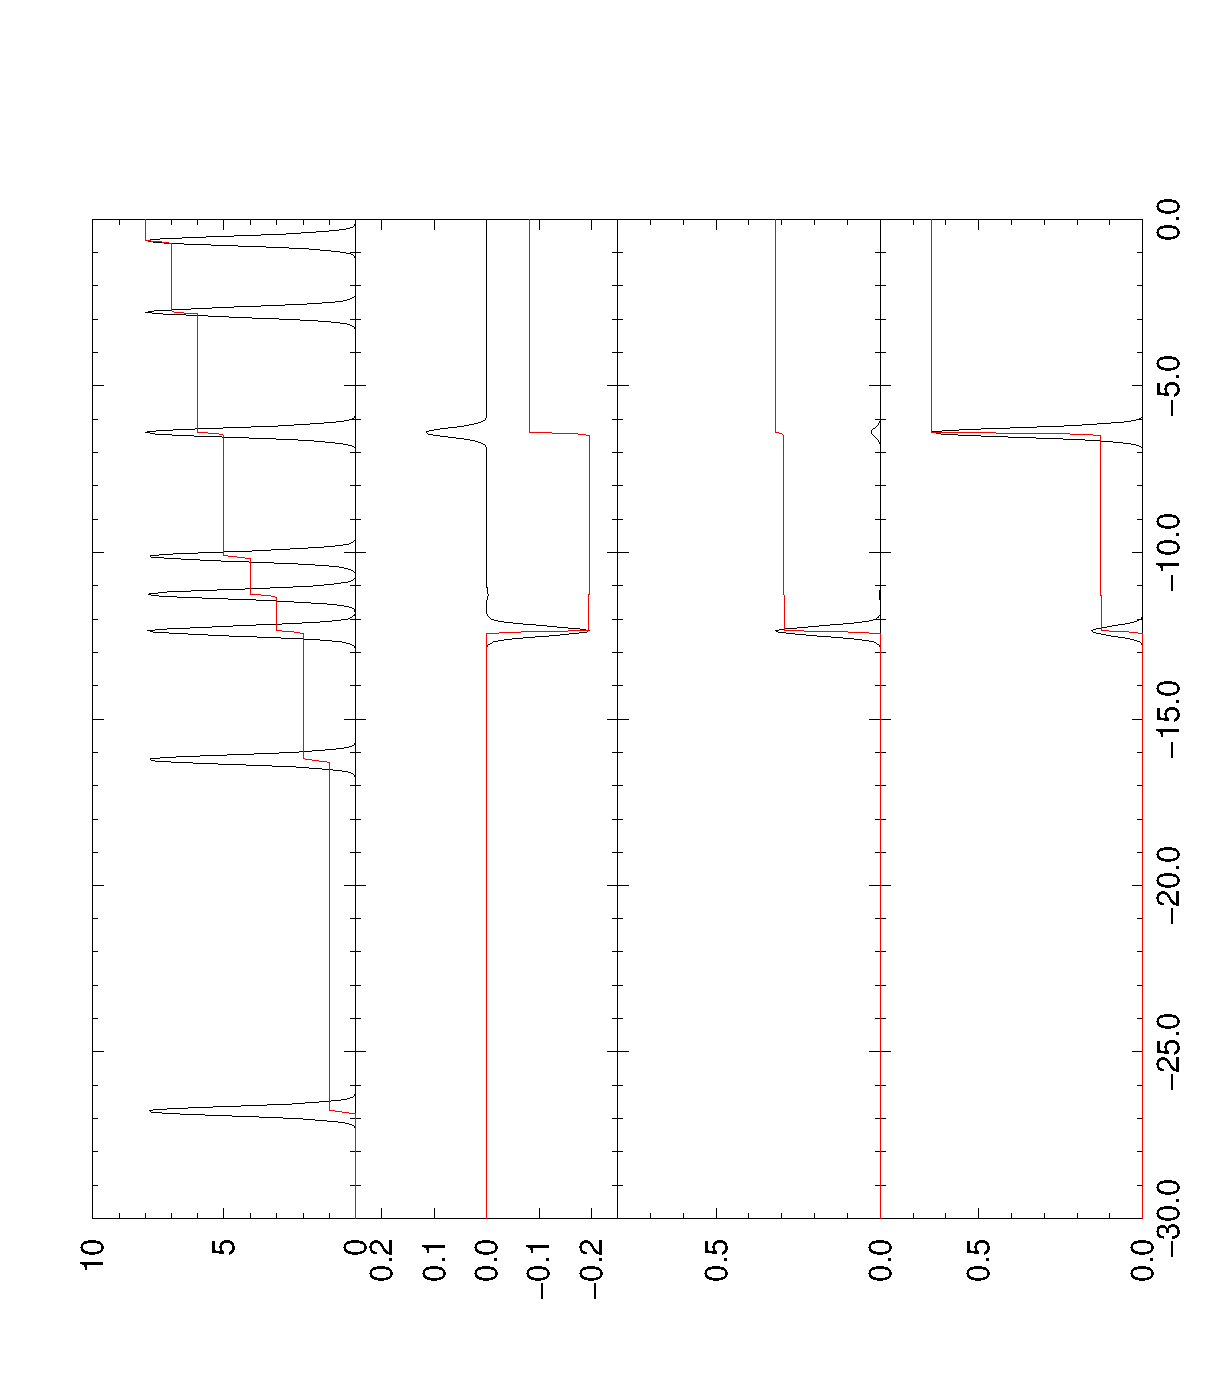
\includegraphics{Figs/h2copdos.eps}}}
\end{center}
 \caption{From top to bottom (1) total density of states of the 
   formaldehyde molecule (H$_2$CO). (2) COOP between the p-orbitals
   lying in the plane of the molecule but perpendicular to the CO
   axis. (3) density of states of the p-orbital contributing to the
   COOP on the carbon atom, (4) density of states of the p-orbital
   contributing to the COOP on the oxygen atom}
\label{fig:h2copdos}
\end{figure}


%==========================================================================
\subsection{Orbital primitives}
\label{sec:dostoolorbitalprimitives}
%==========================================================================
The primitive orbitals are usually partial waves, that are truncated
beyond a certain radius specified in the simulation code.  
\begin{eqnarray}
|\chi_\alpha\rangle=\theta_{\Omega_{R_\alpha}}|\phi_\alpha\rangle
\end{eqnarray}
where $\theta_{\Omega_{R_\alpha}}$ is a real-space step function which is
unity inside some chosen augmentation region and zero elsewhere.  

Per default, the augmentation sphere is confined by the atomic-sphere
radius, is approximately\footnote{The factor corresponds to the ratio
  between the radius of a volume-filling-sphere radius in an fcc
  crystal and the corresponding touching-sphere radius.  The radius of
  a volume filling sphere in an fcc-crystal with lattice constant $1$
  is given by $\frac{4\pi}{4}r^3=\frac{1}{4}$ A touching sphere has
  the radius $r'=1/(2\sqrt{2})$. The ratio is
  $r/r'=\sqrt[3]{\frac{3}{16\pi}}/(\sqrt{2}/4)=1.105$.} 10\% larger
than the covalent radius.  However, it is possible to specify a
different radius in the structure control file of the PAW simulation
code.

In the future, I plan to replace these by local tight-binding orbitals.

%===============================================================================
\subsubsection{Orthonormalization}
%===============================================================================
The orbitals constructed either from truncated orbitals or from
tight-binding orbitals are not orthonormal to other orbitals on the
same site, which produces counterintuitive results.

Therefore, we transform these primitives inside the paw\_dos tool into
a new set that is orthonormal on each site. For this purpose, I
perform a Cholesky decomposition of the overlap matrix of orbitals on
the same site, i.e. $\vec{R}_{\alpha}=\vec{R}_\beta=\vec{R}_\gamma$.
\begin{eqnarray}
\langle\chi_\alpha|\chi_\beta\rangle
=\sum_{\gamma (R_\gamma=R_\alpha)}  L_{\alpha,\gamma}L^\dagger_{\gamma,\beta}
=\sum_{\gamma,\delta}\mat{L}_{\alpha,\gamma}
\langle\chi'_\gamma|\chi'_\delta\rangle
\mat{L}^\dagger_{\delta,\beta}
\qquad\text{for $\vec{R}_\alpha=\vec{R}_\beta$}
\end{eqnarray}
with a lower triangular, real\footnote{The matrix $\mat{L}$ is purely
  real, if the overlap matrix is positive definite, which is always
  satisfied, because the overlap matrix is itself constructed from
  well-defined orbitals.} $\mat{L}$, i.e.
\begin{eqnarray}
L_{\alpha,\beta}=0\qquad\text{for $\beta>\alpha$}
\end{eqnarray}
With $\beta>\alpha$ we refer to the order of partial waves with the
same angular momentum. 

The new set $|\chi'_\alpha\rangle$ obeys local orthonormality
\begin{eqnarray}
\langle\chi'_\gamma|\chi'_\delta\rangle=
\delta_{\gamma,\delta} \qquad\text{for $\vec{R}_\gamma=\vec{R}_\delta$}
\end{eqnarray}

A wave function then has the form
\begin{eqnarray}
|\psi\rangle
&=&\sum_{\alpha}
|\chi_\alpha\rangle_{\Omega_R}
\langle\tilde{\pi}_\alpha|\tilde\psi\rangle
=\sum_{\gamma}
|\chi'_\gamma\rangle_{\Omega_R}
\underbrace{\Bigl(
\sum_{\alpha}
L^\dagger_{\gamma,\alpha}
\langle\tilde{\pi}_\alpha|\tilde\psi\rangle
\Bigr)}_{\langle\tilde{\pi}'_\alpha|\tilde\psi\rangle}
\end{eqnarray}

The new primitive orbitals are
\begin{eqnarray}
|\chi'_\alpha\rangle=\sum_{\gamma=1}^{\alpha}
|\chi_\gamma\rangle L^{\dagger,-1}_{\gamma,\alpha}
\end{eqnarray}
The restriction of the sum over $\gamma$ originates from the fact that
$\mat{L}$ is lower triangular, $\mat{L}^\dagger$ and
$\mat{L}^{\dagger,-a}$ are upper triagonal, so that
$L^{\dagger,-1}_{\gamma,\alpha}=0$ for $\gamma>\alpha$.

%==========================================================================
\subsubsection{Angular-momentum character of orbital primitives}
\label{sec:dostoolorbitalprimitivesangularmomentum}
%==========================================================================
The primitive orbitals are addressed by their angular-momentum
character, where we use real spherical harmonics. Real spherical
harmonics are not angular-momentum eigenstates, but mix states with
$\pm m$. 

Per default, the spherical harmonics are expressed relative to the
cartesian coordinate system used in the calculation.  The angular
momentum character can, however, also be specified with respect to a
arbitrary local coordinate system.

The keywords and their angular momentum character are given in
table~\ref{tab:realsphericalharmonics}. In addition the following
special set of hybrid orbitals can be adressed.
\begin{description}
\item[sp] An sp$^1$ orbital pointing in z-direction: 
$\sqrt{1\over{2}}Y_s \phi_s(|r|) + \sqrt{1\over{2}}Y_{p_z}\phi_p(|r|)$
\item[sp2] An sp$^2$ orbital pointing in z-direction: 
$\sqrt{1\over{3}}Y_s\phi_s(|r|) + \sqrt{2\over{3}}Y_{p_z})\phi_p(|r|)$
\item[sp3] An sp$^3$ orbital pointing in z-direction: 
$\sqrt{1\over{4}}Y_s\phi_s(|r|) + \sqrt{3\over{4}}Y_{p_z})\phi_p(|r|)$
\end{description}

\textcolor{red}{\textbf{CAUTION!} In the present construction, the
  hybrid orbitals are constructed solely from the first partial wave
  of each angular momentum and site. In the presence of semi-core
  states treated as valence, the hybrid orbitals are thus constructed
  from the core states and have no weight from the valence
  states. This is to be changed in the future.}


\begin{table}[!hbt]
\caption{\label{tab:realsphericalharmonics}List of real spherical
  harmonics as they are used in the CP-PAW code. LM is the combined
  angular momentum index used to address the real spherical harmonics
  in the code. $\ell$ is the main angular momentum. $m$ is NOT the
  magnetic quantum number, but a running index within one shell with a
  given main angular monentum. IDs are the names with which the
  orbitals can be addressed. The last column gives the expression of
  the real spherical harmonics in cartesian coordinates.}
\begin{center}
\begin{tabular}{|r|c|c|l|l|}
\hline
LM & $\ell$ & $m$ & IDs & expression \\
\hline
1 & 0 & 1 & S   & $Y_s=\sqrt{1\over{4\pi}}$ \\
\hline
2 & 1 & 1 & PX  & $Y_{p_x}=\sqrt{3\over{4\pi}} {x\over{|r|}}$\\
3 & 1 & 2 & PZ  & $Y_{p_z}=\sqrt{3\over{4\pi}} {z\over{|r|}}$\\
4 & 1 & 3 & PY  & $Y_{p_y}=\sqrt{3\over{4\pi}} {y\over{|r|}}$\\
\hline
5 & 2 & 1  & DX2-Y2
                & $Y_{d_{x^2-y^2}}=\sqrt{15\over{16\pi}} {{x^2-y^2}\over{|r|^2}}$\\
6 & 2 & 2 & DXZ & $Y_{d_{xz}}=\sqrt{60\over{16\pi}} {{xz}\over{|r|^2}}$\\
7 & 2 & 3 & DZ2, D3Z2-R2 
                & $Y_{d_{3z^2-r^2}}=\sqrt{5\over{16\pi}} {{3z^2-r^2}\over{|r|^2}}$\\
8 & 2 & 4 & DYZ & $Y_{d_{yz}}=\sqrt{60\over{16\pi}} {{yz}\over{|r|^2}}$\\
9 & 2 & 5 & DXY & $Y_{d_{xy}}=\sqrt{60\over{16\pi}} {{xy}\over{|r|^2}}$\\
\hline
10 & 3 & 1 & FX(X2-3Y2), F1 
   & $Y_{f_{x(x^2-3y^2)}}=\sqrt{\frac{35}{32\pi}} \frac{x(x^2-3y^2)}{|r|^3}$\\
11 & 3 & 2 & FZ(X2-Y2), F2
   & $Y_{f_{z(x^2-y^2)}}=\sqrt{\frac{210}{32\pi}} \frac{z(x^2-y^2)}{|r|^3}$\\
12 & 3 & 3 & FXZ2, FX(5Z2-R2), F3 
   & $Y_{f_{xz2}}=\sqrt{\frac{21}{32\pi}} \frac{x(5z^2-r^2)}{|r|^3}$\\
13 & 3 & 4 & fZ3, FZ(5Z2-3R2), F4
   & $Y_{f_{z3}}=\sqrt{\frac{14}{32\pi}} \frac{z(5z^2-3r^2)}{|r|^3}$\\
14 & 3 & 5 & FYZ2, FY(5Z2-R2), F4
   & $Y_{f_{yz2}}=\sqrt{\frac{21}{32\pi}} \frac{y(5z^2-r^2)}{|r|^3}$\\
15 & 3 & 6 & FXYZ, F6
   & $Y_{f_{xyz}}=\sqrt{\frac{840}{32\pi}} \frac{xyz}{|r|^3}$\\
16 & 3 & 7 & FY(3X2-Y2), F7
   & $Y_{f_{y(3x^2-y^2)}}=\sqrt{\frac{35}{32\pi}} \frac{y(3x^2-y^2)}{|r|^3}$\\
\hline
\end{tabular}
\end{center}
\end{table}


%==========================================================================
\subsubsection{Spin character of orbital primitives}
%==========================================================================

\textbf{Remark: Currently the spin is a property of the projection and
  not the orbital primitives as it should be.}

For non-collinear electrons the definition of spin-up and spin-down
electrons is ambiguous. The wave function is a \textbf{two-component
  spinor}\index{spinor !two-component} wave function,
\begin{eqnarray}
\left(\begin{array}{c}|\psi(\uparrow,\vec{r})\\\psi(\downarrow,\vec{r})
\end{array}\right)
=\left(\begin{array}{c}\langle\uparrow,\vec{r}|\psi\rangle\\
\langle\downarrow,\vec{r}|\psi\rangle
\end{array}\right)
\end{eqnarray}
I absorbed the spin index $\uparrow/\downarrow$ into the argument
list, in order to differentiate it from a quantum number.\footnote{A
  quantum number $\uparrow$ would characterize an eigenstate of $S_z$
  with eigenvalue $+\hbar/2$. Such a state would have only one
  non-vanishing spinor component,
  i.e. $\psi_\uparrow(\downarrow,\vec{r})=0$.}  A spinor wave function
has a three-dimensional spin-density in each point of
space.\footnote{The term \textbf{``spin density''}\index{spin density}
  is actually a misnomer: It is not the density of spins, but rather a
  \textbf{spin-resolved density}\index{spin-resolved density}.}
\begin{eqnarray}
n_t(\vec{r})
&=&
\psi^*(\uparrow,\vec{r})\psi(\uparrow,\vec{r})  
+\psi^*(\downarrow,\vec{r})\psi(\downarrow,\vec{r})  
\nonumber\\
n_{S_x}(\vec{r})
&=&
\psi^*(\uparrow,\vec{r})\psi(\downarrow,\vec{r})  
+\psi^*(\downarrow,\vec{r})\psi(\uparrow,\vec{r})  
\nonumber\\
n_{S_y}(\vec{r})
&=&
-i\Bigl(
\psi^*(\uparrow,\vec{r})\psi(\downarrow,\vec{r})  
-\psi^*(\downarrow,\vec{r})\psi(\uparrow,\vec{r})  
\Bigr)
\nonumber\\
n_{S_z}(\vec{r})
&=&
\psi^*(\uparrow,\vec{r})\psi(\uparrow,\vec{r})  
-\psi^*(\downarrow,\vec{r})\psi(\downarrow,\vec{r})  
\nonumber\\
\end{eqnarray}

The the representation of a four-component density of states is not
intuitive. Therefore we choose a particular coordinate system and
project onto spin eigenstates along the z-coordinate in this
coordinate system.

For a specific axis $\vec{e}$, the z-axis of the local coordinate
system, the spin eigenstates\footnote{The spin operator along an axis
  $\vec{e}$ with $|\vec{e}|=1$, is
\begin{eqnarray}
S_{\vec{e}}
=\vec{e}\vec{S}
\hat{=}\frac{\hbar}{2}\left(\begin{array}{cc}
e_z & (e_x-ie_y)\\(e_x+ie_y)& -e_z\end{array}\right)
\end{eqnarray}}
 are
\begin{eqnarray}
\left(\begin{array}{c}
\psi_{+e}(\uparrow,\vec{r})\\\psi_{+e}(\downarrow,\vec{r})
\end{array}\right)
&=&
\left(\begin{array}{c}
1+e_z\\x_x+ie_y
\end{array}\right)\frac{f_{+\vec{e}}(\vec{r})}{\sqrt{2(1+e_z)}}
%
\nonumber\\
%
\left(\begin{array}{c}
\psi_{-e}(\uparrow,\vec{r})\\\psi_{+e}(\downarrow,\vec{r})
\end{array}\right)
&=&
\left(\begin{array}{c}
e_x-ie_y\\-(1+e_z)
\end{array}\right)\frac{f_{-\vec{e}}(\vec{r})}{\sqrt{2(1+e_z)}}
\end{eqnarray}
with arbitrary, normalized functions $f_{\pm\vec{e}}(\vec{r})$.
The spin eigenstates obey
\begin{eqnarray}
\vec{e}\hat{\vec{S}}|\psi_{+\vec{e}}\rangle=|\psi_{+\vec{e}}\rangle
\Bigl(+\frac{\hbar}{2}\Bigr)
\nonumber\\
\vec{e}\hat{\vec{S}}|\psi_{-\vec{e}}\rangle=|\psi_{+\vec{e}}\rangle
\Bigl(-\frac{\hbar}{2}\Bigr)
\end{eqnarray}







%==========================================================================
\subsection{Complex orbitals}
%==========================================================================
More complex orbitals such as bond orbitals can be constructed from
these elementary orbitals by using the block ``!DCNTL!ORBITAL''. The
orbitals are named and can be referred to later by their name.

In practice we define the orbital as
$\sum_i|\chi_i\rangle=\sum_j|\phi_j\rangle c_{j,i}$, and
\begin{eqnarray*}
\langle A\rangle\
&=&\sum_{n,i,j}
\langle\tilde{p}_i|\Psi_n\rangle 
f_n\langle\Psi_n|\tilde{p}_j\rangle\langle\phi_j|A|\phi_l\rangle
\\
&=&\sum_{n,i,j,k,l}
\langle\tilde{p}_k|\Psi_n\rangle 
f_n\langle\Psi_n|\tilde{p}_l\rangle
\frac{c_{l,A}c^*_{i,A}}{\sum_m c^*_{m,A}c_{m,A}}
\langle\phi_i|A|\phi_j\rangle
\frac{c_{j,B}c^*_{k,B}}{\sum_m c^*_{m,B}c_{m,B}}
\end{eqnarray*}
which is divided up into into a density matrix and and a matrix
element according to
\begin{eqnarray*}
D_{B,A}&=&\sum_{n,i,j,k,l}
\frac{c^*_{k,B}}{\sum_m c^*_{m,B}c_{m,B}}
\langle\tilde{p}_k|\Psi_n\rangle 
f_n\langle\Psi_n|\tilde{p}_l\rangle
\frac{c_{l,A}}{\sum_m c^*_{m,A}c_{m,A}}
\\
A_{A,B}&=&\sum_{i,j}c^*_{i,A}\langle\phi_i|A|\phi_j\rangle c_{j,B}
\end{eqnarray*}
Thus if we choose a complete set of orthogonal vectors $\{c_{i,u}\}$,
the total expectation value $A$ is recovered by summing the individual
contributions. For an particular atom and orbital, only the first
partial wave is taken as default.

There is one important remark. The projection done here differs from
the projection 
\begin{eqnarray*}
P&=&\frac{|\chi_u\rangle\langle\chi_u|}{\langle\chi_u|\chi_u\rangle}
\\
&=&|\phi_i\rangle 
\frac{\sum_{i,j} c^*_{i,u}c_{j,u}}
{\sum_{k,l}c^*_{k,u}\langle\phi_k|\phi_l\rangle c_{l,u}}\langle\phi_j|
\end{eqnarray*}
that may be anticipated. In this case we would need a set of vectors
normalized with the overlap between partial waves to obtain the
complete result.


%===============================================================================
\subsubsection{Matrix elements}
%===============================================================================

Once the orbitals have been defined, we need to choose the matrix
elements of the PDOS operator. Each matrix element is given a name,
which allows us to use it in further operations. The matrix elements
can be selected in two different ways:

\begin{itemize}

\item To select {\bf diagonal elements} or sums of diagonal elements we use
  the block ``!DCNTL!WEIGHT''. This option allows us to plot the
  total density of states or the angular momentum weights of a
  particular orbital.

\item We can also obtain {\bf off-diagonal elements} using
  ``!DCNTL!COOP'' in order to analyze the bond order or overlap
  populations.

\end{itemize}

%===============================================================================
\subsubsection{Operations}
%===============================================================================
Projected charges, spin and eventually spin directions are printed to
the protocol file.  In order to access the data we have to define how
they are to be represented.
\begin{itemize}
\item We can map the density of states on an energy grid and write the
date to a file, so that they can be plotted.
\item The values at a given energy can be printed to the protocol.
\item The values of a given state can be written to a protocol.
\end{itemize}

%===============================================================================
\subsubsection{Thermal broadening of the Density-of-States}
\label{sec:thermalbroadening}
%===============================================================================
The rationale for the thermal broadening of the density of states is
the following: An expectation value of an observable $A$ can be
written in the form
\begin{eqnarray}
A(\mu)&=&\int_{-\infty}^\infty d\epsilon\; D_A(\epsilon) f_\beta(\epsilon-\mu)
\label{eq:aofmu}
\end{eqnarray}
where $D_A(\epsilon)=\sum_n\frac{1}{V_G}\int d^3k\;
A_n(k)\delta(\epsilon-\epsilon_n(k))$ is a density of states
weighted with the matrix element of $A$ and $f_{\beta}(\epsilon-\mu)$
is the Fermi distribution function.

At zero  temperature, the expectation  value is simply the  integral of
the density of states up to  the Fermi level. A similar expression can
be obtained also for finite temperatures,  if the density of states is
given a thermal broadening.
\begin{eqnarray}
A(\mu)
&=&\int_{-\infty}^\mu d\mu'\;\left.\frac{dA}{d\mu}\right|_{\mu'}
\nonumber\\
&\stackrel{Eq.~\ref{eq:aofmu}}{=}&
\int_{-\infty}^\mu d\mu'\;
\int_{-\infty}^\infty d\epsilon\; D_A(\epsilon) \partial_\mu 
f_\beta(\epsilon-\mu')
\nonumber\\
&=&\int_{-\infty}^\mu d\epsilon\;
\underbrace{
\int_{-\infty}^\infty d\epsilon'\; D_A(\epsilon') \partial_\epsilon 
f_\beta(\epsilon'-\epsilon)}
_{D_A^{\beta}(\epsilon)}
\nonumber\\
&=&\int_{-\infty}^\mu d\epsilon\;D^\beta_A(\epsilon)
\end{eqnarray}
where the thermally smoothened density of states is
\begin{eqnarray}
D_A^{\beta}(\epsilon)
&:=&
\int_{-\infty}^\infty d\epsilon'\; 
\frac{\frac{1}{4}\beta D_A(\epsilon')}
{\cosh^2\Bigl(\frac{1}{2}\beta(\epsilon-\epsilon')\Bigr)}
\end{eqnarray}


The thermal broadening has a second practical reason, namely to
smoothen delta-function like spikes in the density of states resulting
from accidental degeneracies of energies within a tetrahedron, when
the tetrahedron method is used.

If the energies are sampled (MODE='SAMPLE') the result without
broadening is a series of spikes with equal height. Here the broadening
is important to produce a sensible density at the cost of loss of
energy resolution. If sampling is used in a solid, the thermal
broadeing shall mimic an interpolation. Then the broadeing should be
comparable to the typical energy distance of neighboring k-points for
in a typical band.

%===============================================================================
\subsubsection{Format of the Density-of-States and Number-of-States files}
\label{sec:formatdosfile}
%===============================================================================
The density of states file contains the following columns
\begin{enumerate}
\item energy in eV.
\item Density of states. 
\item Density of states weighted with occupations 
\end{enumerate}
For non-collinear spin-polarized calculations, the 
contribution of the spin-$\uparrow$ electrons is drawn first, followed
by that of the spin-$\downarrow$ electrons, drawn with opposite sign. 

The format for the number of states files is analogous.

%==========================================================================
\subsection{Example for the control input file}
%==========================================================================
\begin{verbatim}
!DCNTL
  !FILES 
    !FILE ID='PDOS' EXT=F NAME='~/xx.pdos' !END
    !FILE ID='PROT' EXT=F NAME='stdout'  !END
  !END
  !generic mode='tetra' DOS=T NOS=F prefix='Dos/' !END
  !GRID    DE[EV]=0.1 BROADENING[EV]=0.1 !END
  !ORBITAL NAME='SP3(C1-H2)'
    !ORB ATOM='C_1' TYPE='SP3' NNZ='H_2' FAC=1.0 !END
  !END
  !WEIGHT ID='TOTAL' TYPE='TOTAL' !END
  !WEIGHT ID='W(1)'
     !ORB NAME='SP3(C1-H2)' !END
  !END
  !WEIGHT ID='W(2)'
     !ATOM NAME='C_1' TYPE='ALL'!END
  !END
  !COOP   ID='W(3)'
    !ORB1  NAME='SP3(C1-H2)' !END
    !ORB2  ATOM='H_2' TYPE='S' !END
  !END
!END
\end{verbatim}

%==========================================================================
\newpage
\subsection{Argument description for the control input file}
%==========================================================================

%----------------------------------------------------------------------
\block{!DCNTL}
%----------------------------------------------------------------------
\brules{optional}
\bdescr{defines the operations done on the system; 
largely independent of the system}


%----------------------------------------------------------------------
\block{!DCNTL!GENERIC}
%----------------------------------------------------------------------
\brules{optional}
\bdescr{defines generic settings}

\mbax{\key{MODE}
\vdescr{defines the mode for the calculation of the density of states:
  ``SAMPLE'' uses only the calculated energies on the diskrete k-point
  lattice.  ``TETRA'' denotes the calculation using the tetrahedron
  method.\cite{jepsen71_ssc9_1763, lehmann72_pssb54_469,
    bloechl94_prb49_16223}. \textbf{MODE='SAMPLE' is currently disabled.}}
\vformat{character} 
\vrules{optional}
\vdefault{'TETRA'}}

%% \mbax{\key{DOS} 
%% \vdescr{Density of states will be written to file per default}
%% \vformat{logical} 
%% \vrules{optional}
%% \vdefault{true}}

%% \mbax{\key{NOS} 
%% \vdescr{Number of states will be written to file per default}
%% \vformat{logical} 
%% \vrules{optional}
%% \vdefault{true}}

\mbax{\key{PREFIX} 
\vdescr{String will be prepended to the file names of density of
  states and number of states files}
\vformat{character} 
\vrules{optional}
\vdefault{''}}

%----------------------------------------------------------------------
\block{!DCNTL!GRID}
%----------------------------------------------------------------------
\brules{optional} 
  \bdescr{defines the energy grid and thermal energy
  broadening. The grid extends from the minimum energy value to the
  minimum energy of the highest band.  Read
  section~\ref{sec:thermalbroadening} for the background of the
  thermal broadening.  Large energy gaps are excluded from the grid.}

%% \mbax{\key{EMIN[EV]}
%% \vdescr{lower bound in eV of the energy interval for density 
%% of number of states}
%% \vformat{real} 
%% \vrules{optional}
%% \vdefault{minimum of all energy bands specified on the PDOS file minus
%%   0.1/eV.}}

%% \mbax{\key{EMAX[EV]}
%% \vdescr{upper bound of the energy grid in eV}
%% \vformat{real} 
%% \vrules{optional}
%% \vdefault{minimum of the highest energy band specified on the PDOS
%%   file.}}

\mbax{\key{DE[EV]}
\vdescr{spacing of the grid points on the energy grid in eV. The value
  will be adjusted consistent with an integer number of grid points.}
\vformat{real} 
\vrules{optional}
\vdefault{10$^{-2}$}}

\mbax{\key{BROADENING[EV]}
\vdescr{Thermal broadening $k_BT$ of the density of states expressed in eV. }
\vformat{real} 
\vrules{optional, mutually exclusive with BROADENING[K]}
\vdefault{300 Kelvin/eV}}

\mbax{\key{BROADENING[K]}
\vdescr{Thermal broadening $k_BT$ of the density of states with $T$
  expressed in Kelvin.}
\vformat{real} 
\vrules{optional, mutually exclusive with BROADENING[EV]}
\vdefault{300.}}

%% \mbax{\key{SCALEY} 
%% \vdescr{Obsolete!}
%% \vformat{character} 
%% \vrules{not used}
%% \vdefault{'none'}}

%----------------------------------------------------------------------
\block{!DCNTL!FILES}
%----------------------------------------------------------------------
\brules{optional}
\bdescr{Specifies the file names that deviate from the standard values}

%----------------------------------------------------------------------
\block{!DCNTL!FILES!FILE}
%----------------------------------------------------------------------
\brules{optional, multiple}
\bdescr{Specifies one file}

\mbax{\key{ID}
\vdescr{identifier for the file; options are: 
 \begin{description} 
 \item['PROT']protocol file 
   \hfill\break Standard
   extension:'.dprot'
 \item['ERR']error file
   \hfill\break Standard
   extension:'.derr'
 \item['PDOS'] data file produced by the simulation code. Input for
   paw\_dos tool
   \hfill\break Standard extension:'.pdos'
 \end{description}
}
\vformat{character} 
\vrules{mandatory}
\vdefault{none}}

\mbax{\key{NAME}
\vdescr{filename. Can be the relative file name or an extension to the
  PAW ``root''. Standard output can be specified by NAME='stdout'
  and EXT=.false.}
\vformat{character} 
\vrules{mandatory}
\vdefault{none}}

\mbax{\key{EXT}
\vdescr{.true.: NAME specifies the extension only/ .false.: full name}
\vformat{logical}
\vrules{optional}
\vdefault{.false.}}

%----------------------------------------------------------------------
\block{!DCNTL!ORBITAL}
%----------------------------------------------------------------------
\brules{optional}
\bdescr{defines an orbital}

\mbax{\key{NAME}
\vdescr{names the newly defined orbital !DCNTL!ORBITAL!ORB}
\vformat{character} 
\vrules{mandatory}
\vdefault{none}}

%----------------------------------------------------------------------
\block{!DCNTL!ORBITAL!ORB}
%----------------------------------------------------------------------
\brules{optional, multiple} 
\bdescr{select an orbital (fragment) to be added to the current orbital
\begin{itemize}
\item An elementary unit of a general orbital is a contribution from a
  single site in a specific unit cell. This contribution can be
  specified by an angular momentum character or as hybrid orbital. The
  orbital can be chosen as one of basic types TYPE in a local
  coordinate system.
% 
\item An existing orbital can be selected using NAME. The orbital
  needs to be defined by a preceeding !DCNTL!ORBITAL block. In this
  manner orbitals with arbitrary complexity can be composed.
\end{itemize}
Once defined, the orbital can be shifted by a lattice translation IT
and multiplied with a complex factor FAC.  The orbital primitives are
described further in section~\ref{sec:dostoolorbitalprimitives}.
}

\mbax{\key{NAME}
\vdescr{specifies an orbital previously specified by another block
!DCNTL!ORBITAL!ORB}
\vformat{character} 
\vrules{optional; incompatible with atom and type}
\vdefault{none}}

\mbax{\key{FAC}
\vdescr{Orbital coefficient, with which it contributes to the orbital
  to be built.}
\vformat{complex (real and integer allowed)} 
\vrules{optional}
\vdefault{1.0}}

\mbax{\key{IT}
\vdescr{translations along the three real space lattice vectors. The
  entire orbital is shifted by $\sum_{j=1}^3\vec{T}_j IT_j$.}
\vformat{$3\times$ integer} 
\vrules{optional}
\vdefault{none}}

\mbax{\key{ATOM} 
\vdescr{atom name on which the orbital resides.  (Extended notation,
  see section~\ref{sec:extendedatomnotation} on
  p.~\pageref{sec:extendedatomnotation})}
  \vformat{character}
  \vrules{optional; incompatible with name} 
  \vdefault{none}}

\mbax{\key{TYPE} 
\vdescr{orbital type. Can be one of the following:\\ 'S', 'PX', 'PY',
  'PZ', 'SP1', 'SP2', 'SP3',\\ 'DXY', 'DZ2' or 'D3Z2-R2', 'DXZ',
  'DYZ', 'DX2-Y2',\\ 'FX(X2-3Y2)', 'FZ(X2-Y2)', 'FXZ2' or
  'FZ(5Z2-R2)', 'FZ3' or 'FZ(5Z2-3R2)' 'FXZ2' or 'FY(5Z2-R2)', 'FXYZ',
  'FY(3X2-Y2)'\\ The meaning of these keywords is described in
  section~\ref{sec:dostoolorbitalprimitivesangularmomentum} Only the
  first orbital per angular momentum is used. This omission can be
  undesired, in particular, when core states are treated like valence
  states.}
\vformat{character} 
\vrules{optional; incompatible with name; mandatory if atom is
  specified.}
\vdefault{none}}

\mbax{\key{Z}
\vdescr{vector defining the new z-direction to which TYPE refers}
\vformat{real(3)} 
\vrules{optional (overwritten by NNZ)}
\vdefault{0.0,0.0,1.0}}

\mbax{\key{NNZ}
\vdescr{atom name of the atom to which the vector 
defining the new z-direction points.
(Extended notation, see section~\ref{sec:extendedatomnotation}
on p.~\pageref{sec:extendedatomnotation})}
\vformat{character} 
\vrules{optional; overwrites Z}
\vdefault{see Z}}

\mbax{\key{X}
\vdescr{vector defining the new xz-plane together with z  to which TYPE
refers }
\vformat{real(3)} 
\vrules{optional (overwritten by NNX)}
\vdefault{1.0,0.0,0.0}}

\mbax{\key{NNX}
\vdescr{atom name of the atom to which the vector 
defining the new x-direction points.
(Extended notation, see section~\ref{sec:extendedatomnotation}
on p.~\pageref{sec:extendedatomnotation})}
\vformat{character} 
\vrules{optional; overwrites X}
\vdefault{see X}}

%----------------------------------------------------------------------
\block{!DCNTL!WEIGHT}
%----------------------------------------------------------------------
\brules{optional,multiple}
\bdescr{defines orbital weights; three ways to specify the weights are
possible
\begin{itemize}
\item specify ``TYPE''; rather unspecific selections such as total
  density of states.
\item specify one or several sub-blocks ``!ATOM''; selects
contributions from different atoms.
\item specify one or several sub-blocks ``!ORB''. Most specific
version, identifying individual orbitals
\end{itemize}
The selection type is not compatible with the other two possibilities.
}

\mbax{\key{ID}
\vdescr{defines the name for this set of matrix elements. 
  This ID defines the name of the output file as PREFIX//ID//'.dos', 
  where PREFIX is defined in !DCNTL!GENERIC:PREFIX.
  The file format is described in section~\ref{sec:formatdosfile}}
\vformat{character} 
\vrules{mandatory} 
\vdefault{none}}

\mbax{\key{LEGEND}
\vdescr{defines the legend used in the plot to annotate the dataset.}
\vformat{character} 
\vrules{optional} 
\vdefault{none}}

\mbax{\key{TYPE}
\vdescr{specifies how the weights are defined; can be
\begin{description}
\item[``ALL''] sum over all projected density of states
\item[``EMPTY''] weight of the wave function not considered in any projection
\item[``TOTAL''] total density of states
\end{description}}
\vformat{character} 
\vrules{optional; if type is specified, no blocks !atom or !orbs must
be present}
\vdefault{none}}


\mbax{\key{SPIN} 
\vdescr{specifies the axis $\vec{e}_S$ for the spin projection.  The
  density of states is divided into contributions from eigenstates
  into spin eigenstates parallel and anti-parallel to this spin
  axis. (Even non-spin polarized calculations are interpreted in the 
  data model for non-collinear calculations.) The parallel contribution 
  is shown with positive values and
  the antiparallel contribution is shown with negative values.
\begin{description}
\item['TOTAL'] Both spin components are added up. 
(The second component is set to zero.)
\item['X' or '+X']   spin axis is $\vec{e}_S=(1,0,0)$
\item['-X']   spin axis is $\vec{e}_S=(-1,0,0)$
\item['Y' or '+Y']   spin axis is $\vec{e}_S=(0,1,0)$
\item['-Y']   spin axis is $\vec{e}_S=(0,-1,0)$
\item['Z' or '+Z']   spin axis is $\vec{e}_S=(0,0,1)$
\item['-Z']   spin axis is $\vec{e}_S=(0,0,-1)$
\item['MAIN']  spin axis is the direction of the majority spin axis.
\item[string holding three real numbers] The three numbers are the
  three cartesian components of the spin axis $\vec{e}_S$
\end{description}}
\vformat{character} 
\vrules{optional}
\vdefault{'+Z'}}

%----------------------------------------------------------------------
\block{!DCNTL!WEIGHT!ATOM}
%----------------------------------------------------------------------
\brules{optional}
\bdescr{select the angular momentum weights from a given atom.}

\mbax{\key{NAME}
\vdescr{atom name from which the contribution to this weight is selected}
\vformat{character} 
\vrules{mandatory}
\vdefault{none}}

\mbax{\key{TYPE}
\vdescr{selects the weights from this atom. Can be
\begin{description}
\item[``ALL''] sum over all projected density of states on this atom
\item[``S'']   angular-momentum weight for $\ell=0$
\item[``P'']   angular-momentum weight for $\ell=1$
\item[``D'']   angular-momentum weight for $\ell=2$
\item[``F'']   angular-momentum weight for $\ell=3$
\end{description}
or a combination of S,P,D,F, such as ``SD''.
}
\vformat{character} 
\vrules{optional}
\vdefault{none}}


%----------------------------------------------------------------------
\block{!DCNTL!WEIGHT!ORB}
%----------------------------------------------------------------------
\brules{optional}
\bdescr{usage is same as !DCNTL!ORBITAL!ORB}

%----------------------------------------------------------------------
\block{!DCNTL!COOP}
%----------------------------------------------------------------------
\brules{optional} \bdescr{selects off-diagonal matrix elements of the
  density-of-states operator.  The off-diagonal elements are defined
  by all pairs of orbitals specified in !DCNTL!COOP!ORB1 on the one
  hand and in !DCNTL!COOP!ORB2 on the other hand.

  While it is possible, it is not recommended to use more than one
  pair of orbitals. The result of multiple orbitals is the sum of all
  coops that can be built from orbitals all pairs of orbitals, of
  which one is from ORB1 and the other from ORB2. The result is
  identical to the matrix element of an orbital obtained by summing
  all orbitals ORB1 and another one obtained by summing all orbitals
  ORB2.}

\mbax{\key{ID}
\vdescr{defines the name for this set of matrix elements. 
  This ID defines the name of the output file as PREFIX//ID//'.dos', 
  where PREFIX is defined in !DCNTL!GENERIC:PREFIX.
  The file format is described in section~\ref{sec:formatdosfile}}
\vformat{character} 
\vrules{mandatory} 
\vdefault{none}}

\mbax{\key{LEGEND}
\vdescr{defines the legend used in the plot to annotate the dataset.}
\vformat{character} 
\vrules{optional} 
\vdefault{none}}

\mbax{\key{SPIN} 
\vdescr{specifies the axis $\vec{e}_S$ for the spin projection.  The
  density of states is projected onto contributions from spin eigenstates
  parallel (not antiparallel) to this spin axis. 
(Even non-spin polarized calculations are interpreted in the 
  data model for non-collinear calculations.) 
\begin{description}
\item['TOTAL'] Both spin components are added up. 
(The second component is set to zero.)
\item['X' or '+X']   spin axis is $\vec{e}_S=(1,0,0)$
\item['-X']   spin axis is $\vec{e}_S=(-1,0,0)$
\item['Y' or '+Y']   spin axis is $\vec{e}_S=(0,1,0)$
\item['-Y']   spin axis is $\vec{e}_S=(0,-1,0)$
\item['Z' or '+Z']   spin axis is $\vec{e}_S=(0,0,1)$
\item['-Z']   spin axis is $\vec{e}_S=(0,0,-1)$
\item['MAIN']  spin axis is the direction of the majority spin axis.
\item[string holding three real numbers] The three numbers are the
  three cartesian components of the spin axis $\vec{e}_S$
\end{description}}
\vformat{character} 
\vrules{optional}
\vdefault{'+Z'}}


%----------------------------------------------------------------------
\block{!DCNTL!COOP!ORB1}
%----------------------------------------------------------------------
\brules{optional, multiple} 

\bdescr{selects the 'left' orbital of the density of states matrix
  element Usage is same as !DCNTL!ORBITAL!ORB}

%----------------------------------------------------------------------
\block{!DCNTL!COOP!ORB2}
%----------------------------------------------------------------------
\brules{optional, multiple} 

\bdescr{selects the 'right' orbital of the density of states matrix
  element Usage is same as !DCNTL!ORBITAL!ORB}


%==========================================================================
\newpage
\section{The Density of States Plotting Tool: paw\_dosplot.x}
%==========================================================================
The paw\_dosplot tool prepares a batch file for the plotting software
``Grace''.\cite{xmgrace}. It refers to the output files of paw\_dos
and arranges the data in one or more graphs stacked below each
other. Within a graph several density of states data can be drawn
color coded and stacked ontop of each other


Each \textbf{graph}
is a rectangle containing its own x- and y-axis and it may contain
several sets of Density-of-States.  Graphs are stacked vertically from
top to bottom. All graphs have the same range and ticmarks for the
x-axis.

A \textbf{set} is the content of a \textbf{DoS-file}. The dos file has
the extension '.dos'. Thus a set named 's1' is on the file 's1.dos'.
The x-data are given in eV. 
A DoS-file contains typically four x-y datasets
\begin{enumerate}
\item up-spin filled-and-empty density-of-states,
\item down-spin filled-and-empty density-of-states
\item up-spin filled density-of-states, 
\item down-spin filled density-of-states.
\end{enumerate}
The down-spin density of states has the opposite sign, i.e. it is
multiplied with -1 before it is written to file. The empty density of states
is plotted in lighter color.

The sets are drawn into a graph in sequence, so that the later set
covers the former. With the variable \texttt{STACK=T} the line is
stacked ontop of an existing stack and it is itself added to a
stack. The stack contains at least by the preceeding set.


%==========================================================================
\subsection{Command}
%==========================================================================

The calling sequence is

\bigskip\fbox{{\tt paw\_dosplot} {\it controlfile}}\bigskip

\noindent
where {\it controlfile} is the file name of the control input file for
the paw\_dosplot tool. I recommend the extension ``.dpcntl''.




%==========================================================================
\subsection{Example for the control input file}
%==========================================================================

\begin{verbatim}
!DPCNTL
  EMIN[EV]=-7. EMAX[EV]=25.  YMIN=-0.0 YMAX=0.5  EZERO[EV]=14.
  !GRAPH PREFIX='DOS/'
    !SET ID='TOTAL'  COLOR='BLACK'           !END
    !SET ID='MN_EG'  COLOR='YELLOW'          !END
    !SET ID='MN_T2G' COLOR='GREEN'   STACK=T !END
    !SET ID='PR_F'   COLOR='MAGENTA' STACK=T !END
    !SET ID='PR_D'   COLOR='BLUE'    STACK=T !END
    !SET ID='O'      COLOR='RED'     STACK=T !END
  !END
  !GRAPH PREFIX='DOS/' 
    !SET ID='TOTAL'  COLOR='BLACK'                  !END
    !SET ID='MN_EG'  COLOR='YELLOW'        SCALE=2. !END
    !SET ID='MN_T2G' COLOR='GREEN' STACK=T SCALE=2. !END
  !END
  !GRAPH PREFIX='DOS/'
    !SET ID='TOTAL'  COLOR='BLACK' !END
    !SET ID='MN_T2G' COLOR='GREEN' !END
  !END
!END
!EOB
\end{verbatim}

%==========================================================================
\newpage
\subsection{Argument description for the control input file}
%==========================================================================

%----------------------------------------------------------------------
\block{!DPCNTL}
%----------------------------------------------------------------------
\brules{mandatory}
\bdescr{containes directions on what the tool shall do}

\mbax{\key{EZERO[EV]}
\vdescr{shifts the energy axis of all graphs so the specified value
  (in eV) is the new energy zero. (Often this is chosen as the highest
  occupied state, respectively the Fermi level.) may be overwritten by
  EZERO in !graph and !set}
\vformat{real} 
\vrules{optional}
\vdefault{0.}}


\mbax{\key{EMIN[EV]}
\vdescr{lower bound (in eV) of the energy interval shown}
\vformat{real} 
\vrules{mandatory}
\vdefault{none}}

\mbax{\key{EMAX[EV]}
\vdescr{upper bound (in eV) of the energy interval shown}
\vformat{real} 
\vrules{mandatory}
\vdefault{none}}

\mbax{\key{YMIN}
\vdescr{lower bound in 1/eV of the density-of-states interval shown.  A
  negative value allows to also show the opposite spin direction.}
\vformat{real} 
\vrules{mandatory}
\vdefault{none}}

\mbax{\key{YMAX}
\vdescr{upper bound in 1/eV of the density-of-states interval shown.}
\vformat{real}
\vrules{mandatory}
\vdefault{none}}


%----------------------------------------------------------------------
\block{!DPCNTL!GRAPH}
%----------------------------------------------------------------------
\brules{optional, multiple}
\bdescr{Defines a graph.}

\mbax{\key{PREFIX} 
\vdescr{Default for the prefix used in this graph. The name of the 
  density of states data
  produced by paw\_dos are constructed by appending the prefix
  specified here to the set-id, and by appending the extension
  '.dos'.}
\vformat{character} 
\vrules{optional}
\vdefault{''}}

\mbax{\key{SCALE}
\vdescr{default value for the scale factor of the Density of States 
used in this graph}
\vformat{real} 
\vrules{optional}
\vdefault{1.}}

\mbax{\key{EZERO[EV]}
\vdescr{shifts the energy axis of sets in this graph so the specified
  value (in eV) is the new energy zero.  May be overwritten by EZERO
  in !SET.}
\vformat{real} 
\vrules{optional}
\vdefault{set by !DPCNTL:XZERO}}

\mbax{\key{YMIN}
\vdescr{lower bound in 1/eV of the density-of-states interval shown.  A
  negative value allows to also show the opposite spin direction.}
\vformat{real} 
\vrules{optional}
\vdefault{set by !DPCNTL:YMIN}}

\mbax{\key{YMAX}
\vdescr{upper bound in 1/eV of the density-of-states interval shown.}
\vformat{real}
\vrules{optional}
\vdefault{set by !DPCNTL:YMAX}}


%----------------------------------------------------------------------
\block{!DPCNTL!GRAPH!SET}
%----------------------------------------------------------------------
\brules{optional, multiple}
\bdescr{Defines a set of density of states. A set contains the 
\begin{enumerate}
\item density of states (irrespective of their occupation)
\item density of states weighted with occupation
\end{enumerate}
For collinear spin polarized calculation, the spin-up density is
written first followed by the spin down density.  }

\mbax{\key{ID} 
\vdescr{identifier for set. The name of the density of states data
  produced by paw\_dos are constructed by appending the prefix 
  to the set-id, and by appending the extension
  '.dos'.}
\vformat{character} 
\vrules{mandatory}
\vdefault{none}}

\mbax{\key{PREFIX} 
\vdescr{Prefix used for this set. The name of the density of states data
  produced by paw\_dos are constructed by appending the prefix
  specified here to the set-id, and by appending the extension
  '.dos'.}
\vformat{character} 
\vrules{optional}
\vdefault{is set by !DCNTL!GRAPH:PREFIX}}

\mbax{\key{SCALE}
\vdescr{scale factor of the Density of States used in this graph}
\vformat{real} 
\vrules{optional}
\vdefault{set by !DCNTL!GRAPH:SCALE}}


\mbax{\key{EZERO[EV]}
\vdescr{shifts the energy axis for this set so the specified value (in
  eV) is the new energy zero. }
\vformat{real} 
\vrules{optional}
\vdefault{set by !DPCNTL!GRAPH:XZERO}}

\mbax{\key{STACK}
\vdescr{If true, this set is added ontop of an existing stack. 
This redefines the new set and the stack.
If STACK is non-existent or has the value .false. the stack is reset to the actual set.}
\vformat{logical} 
\vrules{optional}
\vdefault{F}}

\mbax{\key{COLOR} \vdescr{Fills the density of states with
    color. The colors to the left of the following table may be
    used. The corresponding colors on the right will be used for the
    empty density of states.
\definecolor{black     }{RGB}{0  ,  0,  0}      
\definecolor{grey      }{RGB}{200,200,200} 
\definecolor{red       }{RGB}{255,  0,  0}    
\definecolor{green     }{RGB}{  0,230,  0}    
\definecolor{blue      }{RGB}{  0,  0,255}    
\definecolor{yellow    }{RGB}{230,230,  0} 
\definecolor{cyan      }{RGB}{  0,230,230} 
\definecolor{magenta   }{RGB}{255,  0,255} 
\definecolor{orange    }{RGB}{255,165,  0} 
\definecolor{brown     }{RGB}{200,150,150} 
\definecolor{gold      }{RGB}{170,130,  0} 
\definecolor{darkgreen }{RGB}{  0,155,  0} 
\definecolor{lblack    }{RGB}{150,150,150} 
\definecolor{lgrey     }{RGB}{240,240,240} 
\definecolor{lred      }{RGB}{255,150,150} 
\definecolor{lgreen    }{RGB}{170,255,170} 
\definecolor{lblue     }{RGB}{150,150,255} 
\definecolor{lyellow   }{RGB}{255,255,150} 
\definecolor{lcyan     }{RGB}{150,255,255} 
\definecolor{lmagenta  }{RGB}{255,150,255} 
\definecolor{lorange   }{RGB}{255,210,120}
\definecolor{lbrown    }{RGB}{255,180,180} 
\definecolor{lgold     }{RGB}{210,180,100} 
\definecolor{ldarkgreen}{RGB}{120,220,120} 
\begin{center}
\begin{tabular}{|l|c|l|c|}
\hline
name   &RGB &name   &RGB \\
\hline
black     & \colorbox{black     }{\textcolor{white}{(000,000,000)}} 
                                                 & lblack      & \colorbox{lblack    }{(150,150,150)}\\
grey      & \colorbox{grey      }{(200,200,200)} & lgrey       & \colorbox{lgrey     }{(240,240,240)} \\
red       & \colorbox{red       }{(255,000,000)} & lred        & \colorbox{lred      }{(255,150,150)} \\
green     & \colorbox{green     }{(000,230,000)} & lgreen      & \colorbox{lgreen    }{(150,255,150)} \\
blue      & \colorbox{blue      }{\textcolor{white}{(000,000,255)}} 
                                                 & lblue       & \colorbox{lblue     }{(150,150,255)}\\
yellow    & \colorbox{yellow    }{(230,230,000)} & lyellow     & \colorbox{lyellow   }{(255,255,150)} \\
cyan      & \colorbox{cyan      }{(000,230,230)} & lcyan       & \colorbox{lcyan     }{(150,255,255)} \\
magenta   & \colorbox{magenta   }{(255,000,255)} & lmagenta    & \colorbox{lmagenta  }{(255,150,255)} \\
orange    & \colorbox{orange    }{(255,165,000)} & lorange     & \colorbox{lorange   }{(255,210,120)}  \\
brown     & \colorbox{brown     }{(200,150,150)} & lbrown      & \colorbox{lbrown    }{(255,180,180)} \\
gold      & \colorbox{gold      }{(170,130,000)} & lgold       & \colorbox{lgold     }{(210,180,100)} \\
darkgreen & \colorbox{darkgreen }{(000,155,000)} & ldarkgreen  & \colorbox{ldarkgreen}{(120,220,120)} \\
\hline
\end{tabular}
\end{center}
}
\vformat{character} 
\vrules{optional}
\vdefault{''}}


\mbax{\key{LEGEND}
\vdescr{Switch to include a legend-block in the plot when true.}
\vformat{logical} 
\vrules{optional}
\vdefault{.false.}}



%==========================================================================
\newpage
\section{The Band Structure Analysis Tool: paw\_bands}
%==========================================================================
The paw\_bands tool allows one prepare the files for plotting bands
structures including 2-d projected band structures.

%==========================================================================
\subsection{Command}
%==========================================================================

The calling sequence is

\bigskip\fbox{{\tt paw\_bands.x} {\it controlfile}}\bigskip

\noindent
where {\it controlfile} is the file name of the control input file for
the paw\_dos tool. I recommend the extension ``.bcntl''.

%==========================================================================
\subsection{Example for the control input file}
%==========================================================================
An example for the input control file is given here
\begin{verbatim}
!BCNTL
  !INPUTFILE NAME="si.banddata" !END
  !BANDSTRUCTURE_OFF
    METHOD_DIAG=1
    EPWPSI_OFF=10.
    MODE_OFF='LINEARINTERPOLATION'
    MODE='DIAGONALISATION'

    !LINE FILE='BANDS_L_GAMMA_X.DAT'
      KVEC1=0.5 0.5 0.5   
      KVEC2=0. 0. 0. 
      KVECSCALE= 10.3059  
      SPIN=1
      NB=20
      NK=10
      NKDIAG=10
      !FATBAND 
        FILE='FATBANDS_L_GAMMA_X_SI1_IPRO_1.DAT'
        LINESPERBAND=100
        MAXWIDTH=1.0
        ATOM='SI1'
        IPRO=1
      !END
    !END
    !liNE FILE='BANDS_L_GAMMA_X.DAT'
      KVEC1=0. 0. 0. 
      KVEC2=1.0 0.0 0.0   
      KVECSCALE= 10.3059      
      NK=11
      TAPPEND=T
    !END
    !LINE FILE='BANDS_xm.DAT' SPIN=1
      XK1= .5 0. 0. XK2= .5 .5 0. NK=101 
      XKPROJECT= 0. 0. 1.  NPROJECT=11 
    !END
  !END
  !PDOS
    METHOD_DIAG=1
    EPWPSI_OFF=10.
    SPACEGROUP=1
    TSHIFT=F
    NB=20
    NKDIV=7 7 7
  !END
!END
!EOB
\end{verbatim}

\subsection{Description}

The two main tasks that can be accomplished with the paw\_bands-tools are:
\begin{itemize} 
  \item calculation of bandstructures including fat bands and
      projected bandstructures from paw-calculations with either a simple linear
      interpolation scheme on the k-point grid or by a direct diagonalization of
      the paw hamiltonian
  \item calculation of a new pdos-file with different k-points than 
    the ones used in the paw calculation including symmetries
\end{itemize}

For that purpose the control input file is split up into two main sections:
BANDSTRUCTURE and PDOS. Which are connected by the fact that both use the
diagonalisation of the paw hamiltonian.\\ Non-collinear calculations are
currently only partially implemented and  are untested.

\subsubsection{BANDSTRUCTURE}
There are two modes available for the calculation of bandstructures in 
paw\_bands:
\begin{enumerate}
  \item linear interpolation (LINEARINTERPOLATION)
  \item diagonalisation of the paw hamiltonian (DIAGONALISATION)
\end{enumerate}
The first mode one uses a linear interpolation of the energy eigenvalues on the
k-point grid by using the data in the pdos-file, which makes is very fast, but
rather inaccurate. \\ The second one uses an explicit calculation of the energy
eigenvalues of the paw hamiltonian at given k-points. That means that at the
chosen k-points the bandstructure is represented exactly within the accuracy of
the underlying paw calculation. This mode produces very nice bandstructures, but
has a much higher computational demand than the interpolation method, because a
large generalized eigenproblem has to be solved for every k-point. Because of
the high computational demand of diagonalisation, there is also a
mpi-parallelized variant, which is called ppaw\_bands.x and can be compiled
separately with 

\bigskip\fbox{{\tt make bands\_parallel} }\bigskip

\noindent
For computational details see the section about
the theoretical background below.\\
Both variants write the bands are written in the format 
$|\vec k-\vec k_1|\ v_1(\vec k)\ v_2(\vec k)\ v_3(\vec k) \ldots $.\\
 $|\vec k-\vec k_1|$ is the norm of the difference k-vector between 
the k-point $\vec k$ and the first k-point $\vec k_1$ of this 
LINE-block (i.e. kvec1 resp. xk1) in absolute coordinates. $\vec k$ 
goes linearly from $\vec k_1$ to $\vec k_2$ (kvec2 resp. xk2).
The values $v_i(\vec k)$ are either the eigenvalues in eV for the 
$i$-th band or the coordinates for the fat bands if the 
FATBAND-option is used.\\
The plotting of a fat bands is done using a number (LINESPERBAND) of lines,
so that the spread of the lines represents the value of the projection. 
That means that for every band there are LINESPERBAND columns in the file 
instead of one. The calculation of fat bands is currently only implemented
for the calculation of bandstructures via diagonalisation and will
later be extended.\\
The result from the bandstructure calculation can be viewed using 
the program ``xmgrace'' with the command

\bigskip\fbox{{\tt xmgrace -nxy} {\it bands file}}\bigskip

%==========================================================================
\subsubsection{PDOS}
%==========================================================================
This mode allows to recalculate the pdos-file which can the basis to 
calculate (projected) density of states and COOPs with the paw\_dos-tool.
The basic idea is to do a paw calculation as usual, extract the paw 
hamiltonian from that and diagonalize that for a different set of k-points.
In order to reduce the number of k-points it can use the symmetry of the 
crystal, which has to be given in the control input file. Details about 
the symmetry can be found in the section about the theoretical background.
\\
This mode can also be done in a  mpi-parallelized fashion with 
ppaw\_bands.x, which can be compiled separately with 

\bigskip\fbox{{\tt make bands\_parallel} }\bigskip

\noindent
In order to produce a new pdos file, the old pdos-file has to be read.
The new pdos file is written by default to \$ROOT.pdosout, to avoid a 
conflict with the existing pdos from the paw calculation.


%==========================================================================
\subsubsection{Input for a fcc-lattice}
%==========================================================================
Band structure file for the real-space fcc lattice. The real-space
lattice constants are
\begin{eqnarray}
\mat{T}=\left(\begin{array}{ccc}
0,\frac{1}{2},\frac{1}{2}\\
\frac{1}{2},0,\frac{1}{2}\\
\frac{1}{2},\frac{1}{2},0\end{array}
\right)a
\end{eqnarray}
The corresponding reciprocal unit vectors are
\begin{eqnarray}
\mat{g}=\left(\begin{array}{ccc}
-1,1,1\\
1,-1,1\\
1,1,-1
\end{array}\right)\frac{2\pi}{a}
\end{eqnarray}
The high symmetry points are 
\begin{center}
\begin{tabular}{|c|c|c|}
\hline
point & absolute coordinates $\left[\frac{2\pi}{a}\right]$
      & relative coordinates\\
\hline
$\Gamma$ & (0,0,0) & (0,0,0)\\
X        & $(1,0,0)$ &$(0,\frac{1}{2},\frac{1}{2})$\\
W        & $(1,\frac{1}{4},0)$ &$(\frac{1}{8},\frac{1}{2},\frac{5}{8})$\\
L        & $(\frac{1}{2},\frac{1}{2},\frac{1}{2})$ 
              & $(\frac{1}{2},\frac{1}{2},\frac{1}{2})$\\
K        & $(\frac{1}{2},\frac{1}{2},0)$ 
              & $(\frac{1}{4},\frac{1}{4},\frac{1}{2})$\\
U        & $(1,\frac{1}{2},\frac{1}{2})$ 
              & $(\frac{1}{2},\frac{3}{4},\frac{3}{4})$\\
\hline
\end{tabular}
\end{center}
(see \url{https://en.wikipedia.org/wiki/Brillouin_zone})

The high-symmetry path drawn is
\begin{center}
\begin{tabular}{|c|c|c|c|c|c|c|}
\hline
$\Gamma$ & $X$ & $W$           & $L$     & $\Gamma$ & $K$=$U$ &  $X$    \\
\hline
0        & 1   & $\frac{3}{2}$ & 2.20711 & 3.07313  & 4.13379 & 4.48735 \\
\hline
\end{tabular}
\end{center}

The path Gamma-K, U-X is identical to the straight line from
Gamma-point to an X-point of the neighboring cell.


\begin{verbatim}
!bcntl
  !BANDSTRUCTURE MODE='DIAGONALISATION'
    !line comment='gamma-X'
          file='Dos_A/bands.dat' nk=30 NB=8           
          xk1=0. 0. 0. xk2=0.0 0.5 0.5  !end
    !line comment='X-W'
          file='Dos_A/bands.dat' nk=30 NB=8 tappend=T 
          xk1=.0 0.5 0.5 xk2= 0.125 0.5 0.625  !end
    !line comment='W-L'
          file='Dos_A/bands.dat' nk=30 NB=8 tappend=T 
          xk1=0.125 0.5 0.625 xk2= .5 .5 .5   !end
    !line comment='L-Gamma'
          file='Dos_A/bands.dat' nk=30 NB=8 tappend=T 
          xk1= .5 .5 0.5 xk2=0. 0. 0.  !end
    !line comment='Gamma-K'
          file='Dos_A/bands.dat' nk=30 NB=8 tappend=T 
          xk1=0. 0. 0. xk2=.25 .25  .5 !end
    !line comment='U-X'
          file='Dos_A/bands.dat' nk=30 NB=8 tappend=T 
          xk1=0.5 0.75 0.75 xk2= 0.0 0.5 0.5 !end
  !end
!end
!eob
\end{verbatim}


%==========================================================================
\subsection{Argument description for the control input file}
%==========================================================================

%----------------------------------------------------------------------
\block{!BCNTL}
%----------------------------------------------------------------------
\brules{optional}
\bdescr{defines the operations done on the system; 
largely independent of the system}

%----------------------------------------------------------------------
\block{!BCNTL!INPUTFILE}
%----------------------------------------------------------------------
\brules{optional}
\bdescr{Defines banddata file.}

\mbax{\key{NAME}
\vdescr{file name of banddata file from paw calculation.}
\vformat{character} 
\vrules{mandatory}
%\vdefault{If none is specified, the file is the one with extension '.'}
}
%----------------------------------------------------------------------
\block{!BCNTL!BANDSTRUCTURE}
%----------------------------------------------------------------------
\brules{optional}
\bdescr{defines the bandstructure to be computed and plotted including fatbands}

\mbax{\key{mode}
\vdescr{defines the mode of the calculation of the bandstructure. The two
  possible values are 'LINEARINTERPOLATION'' and 'DIAGONALISATION', which are
described below.}
\vformat{character} 
\vrules{optional}
\vdefault{LINEARINTERPOLATION}}

\mbax{\key{method\_diag}
\vdescr{defines the method used for the diagonalisation of the paw hamiltonian 
  (generalized eigenvalue problem). Currently the two Lapack-functions 
zhegvd (method\_diag=1) and zhegv (method\_diag=2) can be used.}
\vformat{integer} 
\vrules{optional}
\vdefault{1}}

\mbax{\key{EPWPSI}
\vdescr{defines the planewave cutoff in Rydberg for the calculation of the 
eigenstates of the paw hamiltonian. The default is to use the same value 
as in the paw calculation, which is stored in the banddata-file.
Details are described below.}
\vformat{real} 
\vrules{optional}
\vdefault{value from paw calculation (from banddata-file)}}

%----------------------------------------------------------------------
\block{!BCNTL!BANDSTRUCTURE!LINE}
%----------------------------------------------------------------------
\brules{optional,multiple}
\bdescr{defines one line segment in k-space, i.e. a part of a bandstructure}

\mbax{\key{XK1} \vdescr{First point of the line segment in relative
    coordinates of the reciprocal lattice vectors. The k-point in
    cartesian coordinates is $\vec{k}$. It is obtained from the
    relative coordinates $\vec{x}$ by multiplication with the
    reciprocal lattice vectors $\vec{g}_1$, $\vec{g}_2$, and
    $\vec{g}_3$as
\begin{eqnarray}
\vec{k}=\vec{g}_1 x_1+\vec{g}_2 x_2+\vec{g}_3 x_3\;.
\end{eqnarray}
}
\vformat{real(3)} 
\vrules{mandatory (xk1 or kvec1)}
\vdefault{none}}

\mbax{\key{KVEC1}
\vdescr{First point of the line segment in cartesian coordinates.}
\vformat{real(3)} 
\vrules{mandatory (xk1 or kvec1)}
\vdefault{none}}

\mbax{\key{XK2}
\vdescr{Last point of the line segment in relative coordinates of the
  reciprocal lattice vectors. See the description of variable $xk1$
  for the relation of absolute and relative coordinates.}
\vformat{real(3)} 
\vrules{mandatory (xk2 or kvec2)}
\vdefault{none}}

\mbax{\key{KVEC2}
\vdescr{Last point of the line segment in cartesian coordinates.}
\vformat{real(3)} 
\vrules{mandatory (xk2 or kvec2)}
\vdefault{none}}

\mbax{\key{KVECSCALE}
\vdescr{scale factor for kvec1 and kvec2 so that they can be given in 
common coordinates, i.e. $\vec k=\frac{2\pi}{kvecscale}\vec k_{input}$.}
\vformat{real} 
\vrules{optional}
\vdefault{$2\pi$}}

\mbax{\key{SPIN}
\vdescr{spin direction. In a spin-polarized collinear 
calculation the parameter can have the values 1 or 2.}
\vformat{integer} 
\vrules{optional}
\vdefault{1}}

\mbax{\key{NK}
\vdescr{number of grid points along the line segment.}
\vformat{integer} 
\vrules{optional}
\vdefault{10}}

\mbax{\key{NKDIAG}
\vdescr{number of grid points along the line segment for diagonalisation. IF
NKDIAG$<$NK the bands obtained from the diagonalisation of the paw hamiltonian
will be interpolated using a 1D-FFT. NKDIAG$>$NK causes an error.}
\vformat{integer} 
\vrules{optional}
\vdefault{NK}}

\mbax{\key{NB}
\vdescr{number of bands}
\vformat{integer} 
\vrules{optional}
\vdefault{20}}

\mbax{\key{XKPROJECT}
\vdescr{direction for the projection for 2-d band structures in relative
coordinates of the reciprocal lattice vectors. Not yet implemented for
METHOD=1.}
\vformat{real(3)} 
\vrules{optional}
\vdefault{(0.,0.,0.)}}

\mbax{\key{NPROJECT}
\vdescr{number of displaced band line segments for the projection 
for 2-d band structures. Not yet implemented for METHOD=1.}
\vformat{integer} 
\vrules{optional, must be an odd number}
\vdefault{1}}

\mbax{\key{FILE}
\vdescr{Output file.}
\vformat{character} 
\vrules{mandatory}
\vdefault{none}}

\mbax{\key{TAPPEND}
\vdescr{If TAPPEND is true, then the output data from the current 
  line segment will be appended at the end of the file FILE. 
  The default behaviour, i.e. when TAPPEND is false 
or not given, an existing file FILE will be overwritten.}
\vformat{logical} 
\vrules{optional}
\vdefault{F}}

%----------------------------------------------------------------------
\block{!BCNTL!BANDSTRCUTURE!LINE!FATBAND}
%----------------------------------------------------------------------
\brules{optional,multiple}
\bdescr{defines an orbital projected band structure (fat bands). This 
rudimentary interface will be extended in the future. Currently only
projections $|\langle\tilde p_{IPRO} |\tilde \psi_i\rangle|^2$ are
used, which are not comparable in magnitude between different IPRO, 
i.e. fatbands of different projectors should not be compared with
respect to their relative magnitude. 
}

\mbax{\key{ATOM}
\vdescr{name of an atom.}
\vformat{character} 
\vrules{mandatory}
\vdefault{none}}

\mbax{\key{IPRO}
\vdescr{number of projector for the calculation of the projected band
structure.} 
\vformat{integer} 
\vrules{mandatory}
\vdefault{none}}

\mbax{\key{LINESPERBAND}
\vdescr{number of lines per band to draw in band structure in order to represent
the value of the projection.} 
\vformat{integer} 
\vrules{optional}
\vdefault{10}}

\mbax{\key{MAXWIDTH}
\vdescr{maximal width in eV of bands in projected band structure.}
\vformat{real} 
\vrules{optional}
\vdefault{1.0}}

\mbax{\key{FILE}
\vdescr{Output file.}
\vformat{character} 
\vrules{mandatory}
\vdefault{data are appended to previously specified file.}}

%----------------------------------------------------------------------
\block{!BCNTL!PDOS}
%----------------------------------------------------------------------
\brules{optional}
\bdescr{defines the calculation of energy eigenvalues and projections, i.e. the
calculation of a new PDOS-file, which is compatible with the one produced from
the main paw program.}

\mbax{\key{NKDIV}
\vdescr{fractions of reciprocal lattice vectors defining the
reciprocal sublattice for the k-points. 
See also !STRUCTURE!KPOINTS!DIV}
  \vformat{integer(3)} 
\vrules{mandatory}}

\mbax{\key{PDOSINFILE}
\vdescr{filename of the PDOS-file to be read.}
\vformat{character} 
\vrules{optional}
\vdefault{\$ROOT.pdos}}

\mbax{\key{PDOSOUTFILE}
\vdescr{filename of the new PDOS-file to be written.}
\vformat{character} 
\vrules{optional}
\vdefault{\$ROOT.pdosout}}

\mbax{\key{NB} 
\vdescr{number of bands. This parameter does not influence the computational
  complexity, because the full spectrum of the paw hamiltonian is calculated. It
only determines the number of bands in the output files.}
\vformat{integer} 
\vformat{integer} 
\vrules{optional}
\vdefault{20}}

\mbax{\key{method\_diag}
\vdescr{see !BCNTL!BANDSTRUCTURE!method\_diag}
\vformat{integer} 
\vrules{optional}
\vdefault{1}}

\mbax{\key{EPWPSI}
\vdescr{see !BCNTL!BANDSTRUCTURE!EPWPSI}
\vformat{real} 
\vrules{optional}
\vdefault{value from paw calculation (from banddata-file)}}

\mbax{\key{SPACEGROUP}
\vdescr{Symmetry of the crystal used for reducing the number of k-points that
have to be calculated. Sequential number according to International Tables for
Crystallography, Vol. A. See description below.}
\vformat{integer} 
\vrules{optional}
\vdefault{1}}

\mbax{\key{TSHIFT}
\vdescr{setting TSHIFT to true excludes the Gamma point from 
  the set of k-points.}
\vformat{logical} 
\vrules{optional}
\vdefault{F}}

\mbax{\key{ISHIFT}
\vdescr{defines a shift of the k-point grid.}
\vformat{integer(3)} 
\vrules{optional}
\vdefault{(0,0,0)}}

%==========================================================================
\subsection{Theoretical background}
%==========================================================================

\subsection{Diagonalisation}
The banddata-file contains all necessary information to build up the
paw hamiltonian $\hat {\tilde H}$ in the plane wave basis. To
calculate the eigenvalues $\epsilon_n $ and eigenstates $|\tilde
\psi_n\rangle$, which are necessary for the projections
$|\langle\tilde p_{IPRO} |\tilde \psi_i\rangle|^2$, we have to solve
the Kohn-Sham equation for the pseudo wave functions:
\begin{equation}
  \hat{\tilde H}|\tilde \psi_n\rangle
=\epsilon_n \hat{\tilde S} |\tilde \psi_n\rangle,
\end{equation}
Here the hamilton operator is given as
\begin{equation}
\hat{\tilde H} 
=\frac{\hat{\vec p}^2}{2}+\tilde v
+\sum_{i,j}|\tilde p_i\rangle
\left(\langle \phi_i|\frac{\hat{\vec p}^2}{2}+v^1|\phi_j\rangle
-\langle \tilde\phi_i|\frac{\hat{\vec p}^2}{2}
+\tilde v^1|\tilde\phi_j\rangle\right)\langle \tilde p_j|
\end{equation}
and the overlap operator can be written as
\begin{equation}
  \hat{\tilde S}
=1+\sum_{i,j}|\tilde p_i\rangle[\langle \phi_i|\phi_j\rangle
-\langle \tilde\phi_i|\tilde\phi_j\rangle]\langle \tilde p_j|.
\end{equation}
(For details please refer to Peter Bl\"ochl's main publication about the paw
formalism.)

For the calculation of the eigenvalues and eigenstates we build up the
operators $\hat{\tilde H}$ and $\hat{\tilde S}$ is a finite plane wave
basis and then solve the resulting generalized eigenvalue problem,
where $\tilde H$ is hermitian and $\tilde S$ is positive definite.

%====================================================================
\paragraph{Matrix dimensions}
%====================================================================
The main part of the computational demand arises from the need to solve the
generalized eigenvalue problem in the plane waves basis. The number of plane
waves, i.e. the dimension $N$ of the matrices of the paw hamilton operator and the
overlap operator scale like $E_{max}^{\frac{3}{2}}$, where $E_{max}$ is the
plane wave energy cutoff (EPWPSI). Also the volume of the simulation cell has a
strong influence. The number of plane waves grows linearly with the real space
volume $V$, i.e. cubic with the lattice parameter.
%====================================================================
\paragraph{Computational demand}
%====================================================================
The computational effect for the full exact diagonalisation of the generalized
eigenvalue problem goes as $N^3$, so that we get an overall runtime of
\begin{equation}
T \in \Theta(E_{max}^{4.5}V^3)
\end{equation}
That means that reducing the plane wave cutoff can dramatically reduce the
computational effort at the expense of accuracy.

\paragraph{Memory demand}
The amount of computer memory need is dominated by the storage requirements for
the matrices, which is $N^2$, because we are using a dense storage format.  So
we get for the memory needed:
\begin{equation}
  M\in \Theta(E_{max}^{3}V^2).
\end{equation}

\subsection{Symmetry}
To reduce the computational effort for the k-point calculations we use the
symmetry of the system, so that only irreducible k-points have to be calculated.
The symmetry group is determined by the parameter SPACEGROUP given in the
PDOS-block, which denotes the three-dimensional spacegroup according to
International Tables for Crystallography, Vol. A. \\
A table of space-group definitions and the corresponding Bravais lattice vectors
can be found in appendix \ref{section:symmetry_tables}.



%==========================================================================
\newpage
\section{The Setup-Analysis program: ``paw\_stpa.x''}
%==========================================================================
Before the simulation starts atomic information is calculated and the
augmentation is constructed. Earlier this was done in an external
program and the information was passed in a file to the simulation code.

During this initialization step a lot of information is created that
is meant to control and to monitor the setup-construction step. This
information is written into a single file in an xml-like format. The
tool ``paw\_stpa.x'', which stands for ``SeTuP-Analysis'', allows to
visualize this information.

%==========================================================================
\subsection{Command}
%==========================================================================

The calling sequence is
\begin{center}
\verb|paw_stpa.x| 
\quad-s\quad\textit{selection}\quad\textrm{-o}\quad\textit{outfile} \quad\textit{file}
\end{center}
where ``\textit{selection}'' is a keyword selecting the information to
be visualized.  The parameter ``\textit{outfile}'' specifies the file
to which the information for the preceeding selection shall be
written. The result is written to standard out, if it is omitted.  The
sequence
``-s\quad\textit{selection}\quad\textrm{-o}\quad\textit{outfile}'' can
be repeated several times.  ``\textit{file}'' is the input file, which
has been written by the paw code. It has the ending
``\verb|stpforz|\textit{Z}\verb|.myxml|'', where \textit{Z} is the
atomic number. The \verb|paw_stpa.x| tool writes the data either in
free format onto single line, or, for array data, the format is
line-by-line free format ``x y1 y2 \ldots''.  It can be visualized for
example with the xy-plotting tool xmgrace.
\begin{center}
\verb|xmgrace -nxy| \textit{out}
\end{center}

Here a list of the parameter ``\textit{selection}'': 
\begin{center}
\begin{tabular}{ll}
 scattering       & phase shifts                                             \\
 nb               & nr. of wave functions                                    \\
 nc               & nr. of core wave functions                               \\
 atom.l           & main angular momenta of wave functions                   \\
 atom.e           & energy eigenvalues in h of wave functions                \\
 atom.f           & occupations of wave functions                            \\
 npro             & nr. of projector functions                               \\
 lpro             & main angular momenta of projector functions              \\
 id               & id of this setup construction                            \\
 z                & atomic number                                            \\
 zv               & nr. of valence electrons                                 \\
 aephi            & all-electron partial waves                               \\
 psphi            & auxiliary partial waves                                  \\
 nlphi            & node-less partial waves                                  \\
 qphi             & core-less partial waves                                  \\
 pro              & projector functions                                      \\
 aephidot         & all-electron scattering partial waves                    \\
 psphidot         & auxiliary scattering partial waves                       \\
 nlphidot         & node-less scattering partial waves                       \\
 pawvalencepsi    & valence wave functions calculated from paw               \\
 aevalencepsi     & all-electron valence wave functions                      \\
 upsi             & node-less wave functions                                 \\
 upsism           & small component of node-less wave functions              \\
 aepsi            & all-electron wave functions                              \\
 aepsism          & small component of all-electron wave functions           \\
 parms.psi.rcl    & method for constructing auxiliary partial waves          \\
 parms.psi.type   & method for constructing auxiliary partial waves          \\
 parms.psi.lambda & decay parameter for constructing auxiliary partial waves \\
 parms.core.rc    & cutoff radius for pseudized core                         \\
 parms.core.pow   & leading power at the origin of the pseudized core        \\
 parms.core.val0  & value at the origin of the pseudized core                \\
 parms.pot.rc     & cutoff radius for pseudized potential                    \\
 parms.pot.pow    & leading power at the origin of the pseudized potential   \\
 parms.pot.val0   & value at the origin of the pseudized potential           \\
 parms.rcsm       & narrow compensation gaussian                             \\
 parms.rbox       & rbox                                                     \\
 pot              & potentials [ae,ps,v(psrho)]                              \\
 prog             & projector functions in g-space                           \\
 vaddg            & vadd in g-space                                          \\
\end{tabular}
\end{center}

 
 
 
 
 
 
 
 
 
 
 
 
 
 
 
 
 
 
 
 
 
 
 
 
 
 
 
 
 
 
 
 
 
 
 
 
 
 
 

%==========================================================================
\newpage
\section{The Structure Pre-Optimization Tool: paw\_preopt}
%==========================================================================

The paw\_preopt tool allows to perform a fast but inaccurate structure
pre-optimization based on force-field molecular dynamics. It reads the
structure input file (\verb'case.strc') and tries to find bonds in the given
structure using the covalent radii of the atoms. Then it tries to find
suitable parameterizations for the atoms using the universal force field (UFF)
\cite{rappe92_jacs114_10024}. (See also section \ref{sec:UFF}.) Bonds and
force field parameterizations can also be provided via the input files. Atoms
to be frozen can be specified.

Using the parameterization it optimizes the geometry (currently) using
the conjugate gradient line search algorithm which is also used in
QM-MM coupling in the main simulation program. Atom positions after
optimization are printed to the protocol file and may be used as
starting point for a PAW simulation.

Atoms can be frozen during the optimization. No other constraints can
be applied. Freezing can either be done via the keywords
!PCNTL!FREEZEONLY and !PCNTL!MOVEONLY or via the keyword FREEZE=T in
the !ATOM block of the structure input file. The latter will be
ignored by the main PAW simulation program.

%==========================================================================
\subsection{Command}
%==========================================================================

The calling sequence is

\bigskip\fbox{{\tt paw\_preopt.x} {\it controlfile}}\bigskip

\noindent
where {\it controlfile} is the file name of the control input file for
the paw\_preopt tool. I recommend the extension ``.pcntl''.

%==========================================================================
\subsection{Example for the control input file}
%==========================================================================

\begin{verbatim}
!PCNTL
  !FILES
    !FILE ID='xyz' NAME='optimized.xyz' !END
  !END
  !GENERIC
    TRACE=F
    TOL=0.0001
    NSTEPS=10000
  !END
  !OUTPUT
     PRINTATOMS=T
     PRINTBONDS=T
     WARNFF=T
     XYZOUT=T
  !END
  !FREEZEONLY 
    COMMENT='Not used if MOVEONLY is present.'
    !ATOM NAME='MO1' !END
    !ATOM PART='FE' !END
  !END
  !MOVEONLY
     !ATOM_OFF PART='H_nh' !END
     !ATOM NAME='N_nh41' !END
     !ATOM NAME='H_nh43' !END
     !ATOM NAME='H_nh44' !END
     !ATOM NAME='H_nh45' !END
  !END
!END
!EOB
\end{verbatim}

Please note that a keyword COMMENT is ignored by all PAW
programs. Thus it can be used to add comments to the input files.






%==========================================================================
%\newpage
\subsection{Argument description for the control input file}
%==========================================================================

%----------------------------------------------------------------------
\block{!PCNTL}
%----------------------------------------------------------------------
\brules{mandatory}
\bdescr{defines the operations done on the system; 
largely independent of the system}

%----------------------------------------------------------------------
\block{!PCNTL!GENERIC}
%----------------------------------------------------------------------
\brules{optional}
\bdescr{defines optimization parameters (and use of the trace)}

\mbax{\key{TRACE}
\vdescr{writes information on the calls of subroutines to standard output}
\vformat{logical} 
\vrules{optional}
\vdefault{F}}

\mbax{\key{TOL}
 \vdescr{tolerance of the maximal component of the force on atoms in 
  the convergence cycles}
\vformat{real} 
\vrules{optional}
\vdefault{10$^{-4}$}}

\mbax{\key{NSTEPS}
\vdescr{maximal number of steps for the convergence. After that number
  the structure optimization is stopped no matter if the forces have
  become smaller than TOL. A statement on the convergence will be
  written to the protocol.}
\vformat{integer} 
\vrules{optional}
\vdefault{1000}}

%----------------------------------------------------------------------
\block{!PCNTL!FILES}
%----------------------------------------------------------------------
\brules{optional}
\bdescr{specifies the file names that deviate from the standard values}

%----------------------------------------------------------------------
\block{!PCNTL!FILES!FILE}
%----------------------------------------------------------------------
\brules{optional, multiple}
\bdescr{Specifies one file}

\mbax{\key{ID}
\vdescr{identifier for the file; options are: 
 \begin{description} 
 \item['PROT']protocol file \hfill\break Standard extension:'.pprot'
 \item['STRC'] The structure file as used by the simulation code. Used
   for the input structure. \hfill\break Standard extension:'.strc'
 \item['XYZ'] data file with the resulting optimized structure
   \hfill\break Standard extension:'.xyz'
 \end{description}
}
\vformat{character} 
\vrules{mandatory}
\vdefault{none}}

\mbax{\key{NAME}
\vdescr{filename. Can be the relative file name or an extension to the
  PAW ``root''. Standard output can be specified by NAME='stdout'
  and EXT=.false.}
\vformat{character} 
\vrules{mandatory}
\vdefault{none}}

\mbax{\key{EXT}
\vdescr{T: NAME specifies the extension only. F: full name}
\vformat{logical}
\vrules{optional}
\vdefault{F (false)}}

%----------------------------------------------------------------------
\block{!PCNTL!OUTPUT}
%----------------------------------------------------------------------
\brules{optional}
\bdescr{specifies which information should be written to the protocol}

\mbax{\key{PRINTATOMS}
\vdescr{information on the used atom parameterization and freezing is
  written to the protocol}
\vformat{logical} 
\vrules{optional}
\vdefault{T}}

\mbax{\key{PRINTBONDS}
\vdescr{information on the used bonds is
  written to the protocol}
\vformat{logical} 
\vrules{optional}
\vdefault{T}}

\mbax{\key{WARNFF}
\vdescr{paw\_preopt tries to find best-suiting force fields for the
  atoms. However, in some cases it cannot decide which parameterization
  will be the best. If T in these cases a warning will be printed to
  the protocol.}
\vformat{logical} 
\vrules{optional}
\vdefault{T}}

\mbax{\key{XYZOUT}
\vdescr{should an xyz-file of the resulting structure be created?}
\vformat{logical} 
\vrules{optional}
\vdefault{T}}


%----------------------------------------------------------------------
\block{!PCNTL!FREEZEONLY}
%----------------------------------------------------------------------
\brules{optional, not used if !PCNTL!MOVEONLY is present}
\bdescr{sets freezing of all atoms but those specified in this block
  to false. May be overwritten for single atoms by !STRC!ATOM:FREEZE}

\mbax{\key{NAME}
\vdescr{specifies an atom name}
\vformat{character} 
\vrules{optional, multiple}
\vdefault{none}}

\mbax{\key{PART}
\vdescr{Specifies a part of an atom name. All atoms containing this
  string are used. Case is ignored.}
\vformat{character} 
\vrules{optional, multiple}
\vdefault{none}}

%----------------------------------------------------------------------
\block{!PCNTL!MOVEONLY}
%----------------------------------------------------------------------
\brules{optional, overwrites !PCNTL!FREEZEONLY}
\bdescr{sets freezing of all atoms but those specified in this block
  to true. May be overwritten for single atoms by !STRC!ATOM:FREEZE}

\mbax{\key{NAME}
\vdescr{specifies an atom name}
\vformat{character} 
\vrules{optional, multiple}
\vdefault{none}}

\mbax{\key{PART}
\vdescr{Specifies a part of an atom name. All atoms containing this
  string are used. Case is ignored.}
\vformat{character} 
\vrules{optional, multiple}
\vdefault{none}}

%==========================================================================
%\newpage
\subsection{Argument description for the structure input file}
%==========================================================================

The atomic structure is read from a structure input file which has the
same syntax as for the main simulation code. However, a few keywords
are used which are ignored by the main simulation code. The keyword
!STRC!GENERIC:LUNIT is mandatory.

%----------------------------------------------------------------------
\block{!STRC!ATOM}
%----------------------------------------------------------------------
\brules{mandatory,multiple}
\bdescr{usage is same as in the main simulation code. Keywords R, SP
  and NAME are used. Additional keywords are:}

\mbax{\key{FFTYPE}
\vdescr{Force field type used for this atom. This keyword can be used
  to overwrite the suggestion of the program. Possible force fields
  can be found in section~\ref{sec:UFF} on page~\pageref{sec:uff}.}
\vformat{character} 
\vrules{optional}
\vdefault{depending on the atom type and the number of bonds to that atom}}

\mbax{\key{FREEZE}
\vdescr{freeze this atom}
\vformat{logical} 
\vrules{optional}
\vdefault{F}}

%----------------------------------------------------------------------
\block{!STRC!BOND}
%----------------------------------------------------------------------
\brules{optional,multiple}
\bdescr{Overwrite the suggestion of the program for bonds between the
  atoms. Not yet implemented.}

 
%==========================================================================
\newpage
\section{Structure converter Tool: paw\_fromposcar.x}
%==========================================================================
This tool facilitates the input of atomic structures by converting the
widespread format 'POSCAR' of the VASP code\footnote{The POSCAR format
  changed with version 5 of VASP. The new version is implemented.}
into the format used by the structure input file of CP-PAW.

Source of atomic structures are
\begin{itemize}
\item ``The Materials Project''
\url{https://materialsproject.org}, which is a collection of
electronic structure calculations already done.
%
\item The AFLOW standard library of crystallographic prototypes
  \url{http://aflowlib.org/CrystalDatabase/}
\end{itemize}

%==========================================================================
\subsection{Command}
%==========================================================================

The calling sequence is\bigskip

\fbox{{\tt paw\_fromposcar.x} \textit{poscar-file-name} 
[\textit{lunit}]}\bigskip

\noindent or\bigskip

\fbox{{\tt paw\_fromposcar.x} -h}
\bigskip

\noindent
where 
\begin{itemize}
\item \textit{poscar-file-name} is the name of the poscar input file, 
\item the optional argument \textit{lunit} is the length unit used in
  the out file.
\item The result, the structure in CP-PAW style, is written to stdout
  (standard out) and can thus be piped '$>>$' into a structure file,
  which is in preparation. Note that editing of the striucture file is
  required.
\item If the first argument is '-h', the usage information is written
  to stdout.
\end{itemize}

%==========================================================================
\newpage
\section{Scripts}
%==========================================================================
The scripts are small bash shell scripts that simplify recurring operations
with the CP-PAW code. 

The following table provides an overview:\\
\begin{center}
\begin{tabular}{ll}
\verb|paw_do|      & frontend for paw calculations and tools. \\
\verb|paw_show|    & show energies vs iterations. \\
\verb|paw_collect| & collect total energies. \\
\verb|paw_get|     & extract the last value of certain data from simulation.\\
\verb|paw_copy|    & copy files into ones with a different root name.\\
\verb|paw_ext_copy|& copies files into ones with a different extension\\
\verb|paw_resolve| & expand text files according to replacement rules.\\
\verb|paw_scan|    & perform sequence paw calculation \\
\verb|paw_scanlat| & scan lattice constants. \\
\verb|paw_getsrc.sh| & extract source blob from executable\\
\end{tabular}
\end{center}

%==========================================================================
\subsection{Options and \textit{getopts}}
%==========================================================================
While there are currently a few exceptions, the options are scanned by
the bash command \textit{getopts}. This implies that the options have
the form of a single letter followed by an optional one-word
argument. If the one-word argument is a sequence, enclose them by
apostrophes. The string ``word1 word2 word3'' is treated as one-word
argument.  The option id's can be arranged in arbitrary order and they
can be grouped together. The optional argument may directly follow its
option id or it may be separated from it by spaces.

%==========================================================================
\subsection{The Frontend Tool: ``paw\_do''}
\label{sec:pawshow}
%==========================================================================
The tool paw\_do simplifies a number of standard operations.  It It
assumes that there is exactly one PAW project in the current
directory.  It exploits the notion of standard extensions and can
already process a number of commands. By changing a one-letter
optional argument, various tasks can be done with the same argument.


%==========================================================================
\subsubsection{Command}
%==========================================================================

The calling sequence is

\bigskip\fbox{{\tt paw\_do\ } {\it option}}\bigskip

\begin{description}
\item[-h] print this help message
\item[-A] paw\_show -ce ROOT
\item[-B] paw\_bands.x ROOT.bcntl; xmgrace -nxy bands.dat
\item[-F] paw\_fast.x ROOT.cntl 
\item[-D] paw\_dos.x ROOT.dcntl; paw\_dosplot.x ROOT.dpcntl; 
  xmgrace -batch ROOT.bat
\item[-K] touch ROOT.exit (regular stop of simulation)
\item[-P] doppaw ROOT 4 (parallel ppaw\_fast.x with 4 tasks)
\item[-S] paw\_strc.x -c ROOT
\item[-T] paw\_tra.x ROOT.tcntl
\item[-W] paw\_wave.x ROOT.wcntl
\item[-Z] tail -f ROOT.prot
\item[-0] dry-run (creates files but does not run jobs)
\item[-v] verbose
\end{description}

ROOT is the root name of the current project. It is extracted from a
search of all files with the required extension in the current
directory.  The tool assumes that the ROOT is unambiguous in the
current directory.

%==========================================================================
\subsection{The Energy Analysis Tool: ``paw\_show''}
\label{sec:pawshow}
%==========================================================================
The tool paw\_show allows one to inspect the protocol file. It plots the
total energy, the instantaneous temperature of the atoms, the
fictitious kinetic energy of the wave functions, the conserved energy
versus the time step in picoseconds. This tool requires the xmgr plot
library\cite{xmgrace}.

%==========================================================================
\subsubsection{Command}
%==========================================================================

The calling sequence is

\bigskip\fbox{{\tt paw\_show\ } {\it option\  rootname file}}\bigskip

\noindent where {\it rootname} is the name of the protocol file 
without the ``.prot'' ending and {\it option} is one of the following:
\begin{description}
\item[-f] fictitious kinetic energy of the wave functions
\item[-e] the static total energy
\item[-c] the conserved energy
\item[-t] temperature of the atoms in Kelvin
\item[-ar] friction parameter for the atoms
\item[-ap] friction parameter for the wave functions
\item[-s] use time steps instead of time in ps
\item[-u unit] select unit (h, ry, ev, kj/mol, kcal/mol)     
\item[-h] prints information about usage of the tool 
\item[?] prints information about usage of the tool 
\end{description}
The optional parameter {\it file} the file to which the data are
written. If {\it file} is absent, the data are viewed.


%==========================================================================
\subsection{Copy a project: ``paw\_copy''}
%==========================================================================
paw\_copy makes a copy of a cp-paw project with a new rootname.


%==========================================================================
\subsubsection{Command}
%==========================================================================
The calling sequence is

\bigskip\fbox{{\tt paw\_copy\ } {\it root1 root2}}\bigskip

\noindent where {\it root1} is the root name of the project to be
copied and root2 is the target foot name.

Specifically, it takes all files beginning with {\it root1} in the
current directory and copies the files with the same name but {\it
root1} replaced by {\it root2}.

%==========================================================================
\subsection{change the extension  of a et of files: ``paw\_ext\_copy''}
%==========================================================================
paw\_ext\_copy makes a copies of a set of files with a given ending (extension) into files with the same beginning, but a different extension.


%==========================================================================
\subsubsection{Command}
%==========================================================================
The calling sequence is

\bigskip\fbox{{\tt paw\_ext\_copy\ } {\it ext1 ext2}}\bigskip

\noindent where {\it ext1} is the extension of the files to be
copied and \textit{ext2} is the target extension.

Specifically, it takes all files ending with \textit{ext1} in the
current directory and copies the files with the same name but
\textit{ext1} replaced by \textit{ext2}.

%==========================================================================
\subsection{Collect energies ``paw\_collect''}
%==========================================================================
paw\_collect collects the last total energies from all protocoll files
in the current directory.

%==========================================================================
\subsubsection{Command}
%==========================================================================
The calling sequence is

\bigskip\fbox{{\tt paw\_collect\ }}

%==========================================================================
\subsection{Collect energies ``paw\_get''}
%==========================================================================
paw\_get extracts the final result of various energies from the
protocoll file.

%==========================================================================
\subsubsection{Command}
%==========================================================================
The calling sequence is

\bigskip\fbox{{\tt paw\_get} \textit{options} \textit{ROOTNAME}}
\vspace{0.5cm}

\noindent Options:\\[2mm]
\hspace*{1cm}\fbox{\begin{minipage}{0.9\linewidth}
\begin{description}
\item[-h:] print help message
\item[-w whatid:] Specify the quantity to be extracted. whatid may be one of
\begin{description}
\item[etot:] total energy 
\item[gap:]  fundamental band gap 
\item[homo:] energy of the highest occupied state
\item[lumo:] energy of the lowest unoccupied state
\item[efermi:] energy of the fermi level 
\item[volume:] unit cell volume
\item[epw:] wave function plane wave cutoff
\item[epwrho:] density plane wave cutoff
\item[nkpt:] number of k-points
\end{description}
\item[-u:] unit (1, ev, kj/mol, kcal/mol , H, angstrom\^{}3, aa\^{}3,
  cubangstrom, a0\^{}3, abohr\^{}3, cubabohr) case insensitive. Unit must
  be consistent with quantity to be retrieved
\item[-n:] prints the result as number 
\item[-t:] prints the result as text
\item[-v:] verbose
\end{description}
\end{minipage}}
\bigskip

The command scans the file \textit{rootname}\verb|.prot| and
prints the last occurance of the corresponding variable.

Remark: -gap does not work with variable occupations and will provide
an error message. -lumo and -homo will report the chemical potential
with variable occupations.
%
%==========================================================================
\subsection{Collect energies ``paw\_resolve''}
%==========================================================================
paw\_resolve constructs \textit{outfile} from \textit{infile} by
replacing specific placeholders either by a specific value or by the
contents of a specified file. 

It is typically used within shell scripts to scan certain variable
sets in the structure or control files of a PAW calculation.  For
example a string ``EPW=@X1@'' will be changed with the replacement
rule ``X1=30'' to ``EPW=30''. Several such rules can be specified.

There are also replacement rules that insert complete files. Here one
introduces a single line containing the id of the file-replacement
rule.  This line will be replaced by the content of the file. This
allows one to exchange for example the setup information consistently
in a group of projects.

%==========================================================================
\subsubsection{Command}
%==========================================================================
The calling sequence is

\bigskip\fbox{{\tt paw\_resolve} \textit{options} \textit{infile}
$>$\textit{outfile}}
\vspace{0.5cm}

\noindent Options:\\[2mm]
\hspace*{1cm}\fbox{\begin{minipage}{0.9\linewidth}
\begin{description}
\item[-h:] print help message
\item[-p prefix:] prefix to be added to the filename in @file@
\item[-r id=value:] rule to convert @id@ into value
\item[-f id=file:] rule to replace lines containing @id@ by the contents of file
\end{description}
\end{minipage}}
\bigskip
%
%==========================================================================
\subsection{Scan parameters ``paw\_scan''}
%==========================================================================
A typical application is to scan a certain parameter value

%==========================================================================
\subsubsection{Command}
%==========================================================================
The calling sequence is

\bigskip\fbox{{\tt paw\_scan} \textit{options}  SRCROOT}
\vspace{0.5cm}

\noindent Options:\\[2mm]
\hspace*{1cm}\fbox{\begin{minipage}{0.9\linewidth}
\begin{description}
\item[-h:] print help message
\item[-r ``name value1 value2 ...'':] replacement rule
\item[-w \textit{whatid}:] 
\begin{description}
\item[\textit{whatid}=run:] perform CP-PAW simulation. Requires .cntl and .strc files
\item[\textit{whatid}=fast:] perform CP-PAW simulation Requires .cntl and .strc files
\item[\textit{whatid}=dos:]make density-of-states. Requires .dcntl file.
\end{description}
\item[-n \textit{nnodes}:] submit parallel job with the number of processes specified by \textit{nnodes}.
\item[-m \textit{hostname}:] limit execution to the specified host
  \textit{hostname}
\item[-0:] dry-run (creates files but does not run jobs)
\item[-b \textit{directory}:] directory containing the paw executables
\item[-v:] verbose
\end{description}
the argument SRCROOT is the rootname of the source files and
 the common part of the root name for all projects.
 It must contain the a relative or absolute path (i.e. one "/")..
 The root names of individual projects will be formed as
 TARGETROOT=\$SRCROOT\_\$VALUE/\$PROJECT\_\$VALUE.
 where PROJECT is \$SRCROOT stripped of the directory part
 and VALUE is assigned by the rule specified by option -r.

 If the target directory does not contain a restart file,
 a source restart file \$SRCROOT.rstrt, if present and needed,
 will be copied into the target directory.

 Example:
%\begin{verbatim}
 	 paw\_scan -w run -r "EPW 20 30 40" ./si2
%\end{verbatim}
\end{minipage}}

\bigskip
\noindent Preconditions:\\[2mm]
\hspace*{1cm}\fbox{\begin{minipage}{0.9\linewidth}
\begin{itemize}
\item 	 projectname.cntl
\item 	 projectname.strc
\end{itemize}
\end{minipage}}
\bigskip
%
%==========================================================================
\subsection{Scan lattice constants ``paw\_scanlat''}
%==========================================================================
A typical application is to calculate the energy versus volume
dependence, which yields the equilibrium lattice constant and the bulk
modulus. 

%==========================================================================
\subsubsection{Command}
%==========================================================================
The calling sequence is

\bigskip\fbox{{\tt paw\_scanlat} \textit{options} }
\vspace{0.5cm}

\noindent Options:\\[2mm]
\hspace*{1cm}\fbox{\begin{minipage}{0.9\linewidth}
\begin{description}
\item[-l \textit{list}:] list of percent changes of the lattice
  constant (enter in apostrophes "...")\\
  default: {\tt ``96 97 98 99 100 101 102 103 104"}
%
\item[-p \textit{rootname}:] rootname of the project to be considered
  (mandatory)
%
\item[-u:] update only. No paw simulation.
%
\item[-e \textit{executable}:] name of the executable\\
    default: {\tt |"paw\_waittillempty -n \$NJOBS ; paw\_fast"|}
%
\item[-j \textit{n}:] $n$ paw jobs are allowed to run
   simultaneously. Only used when option {\tt -e} is absent.
%
\item[-h:] print help message
\item[-v:] verbose
\item[-0:] dry run
\end{description}
\end{minipage}}\\
\bigskip

\noindent Preconditions:\\[2mm]
\hspace*{1cm}\fbox{\begin{minipage}{0.9\linewidth}
\begin{itemize}
\item 	 projectname.cntl
\item 	 projectname.strc
\end{itemize}
\end{minipage}}
\bigskip

\noindent Example:\\[2mm]
\begin{verbatim}
paw_scanlat -u -l "96 98 100 102 104" -p nio \
            -e "waittillempty -n 4; paw_fast.x"
\end{verbatim}

\noindent Explanation:\\[2mm]
\verb|paw_scanlat| makes copies of the control, structure and restart
files of the project with
\begin{itemize}
\item the values specified by option \verb|-l| appended to the project
  name and
\item the length unit scaled by the percentage values specified by option
  \verb|-l| appended to the project.
\end{itemize}
and performs paw calculations.  The restart file is copied only if it
does not yet exist.

Finally \verb|paw_scanlat| extracts the total energies. It produces
two files:
\begin{itemize}
\item \verb|etot.dat| containing a two-column list of (1) percentage
  scaling specified by the option \verb|-l| and (2) the energy in
  Hartree.  
\item \verb|murn.in| containing a two-column list of (1) the cube of
  the length unit in the in abohr and (2) the energy in Hartree. This
  file is used as input file for the \verb|paw_murnaghan.x.| tool
\end{itemize}




%==========================================================================
\subsection{Murnaghan fit ``paw\_murnagan.x''}
%==========================================================================
{\tt paw\_murnaghan.x} extracts the minimum energy, equilibrium
volume, bulk modulus and its pressure derivative from a
energy-vs-volume data sequence. The equation of state proposed by
Murnaghan\cite{murnaghan44_pnas30_244} is based on the assumption that
the bulk modulus depends linearly on pressure.

The calling sequence is

\bigskip\fbox{{\tt paw\_murnaghan.x\ < murn.in}}\bigskip

where {\tt in.dat} is an input file holding the energy-versus-volume
data.  The first column of {\tt in.dat} holds the volumes and the
second the corresponding energies, both given in Hartree atomic
units. 



In addition a file ``{\tt murn.dat}'' is produced holding the
interpolated data covering the range of the input volumes +10\%.


%==========================================================================
\subsubsection{Command}
%==========================================================================
The calling sequence is

\bigskip\fbox{{\tt paw\_murnaghan.x} \textit{options} < murn.in}
\vspace{0.5cm}

\noindent Options:\\[2mm]
\hspace*{1cm}\fbox{\begin{minipage}{0.9\linewidth}
\begin{description}
\item[-l:] first column of input is a length $L$.
%   
\item[-v:] (default) first column of input is a volume. $L^3$
%
\item[-eu \textit{value}:] energy unit of second column in
  Hartree. default: 1.
%
\item[-lu \textit{value}:] length unit of the data in the first column
  in abohr. Default: 1.
%
\item[-vbl \value{value}:] Volume $\det[T]/L^3$ of the unit cell
  expressed in length units $L$. $T/L$ is the matrix of the three
  lattice vectors as specified in {\tt !STRUCTURE!LATTICE:T=}. Default: 1.
%
\item[-scale \textit{value}:] energies and volumes are scaled by this
  value.  If the unit cell contains, for example, two formula units,
  the results for one formula unit are obtained using a scale factor of
  0.5. Input data are scaled upon reading.
%
\item[-h:] print help message
\item[-v:] verbose
\item[-0:] dry run
\end{description}
\end{minipage}}\\
\bigskip

\noindent Preconditions:\\[2mm]
\hspace*{1cm}\fbox{\begin{minipage}{0.9\linewidth}
\begin{itemize}
\item 	 murn.in (File to be passed to standard in).
\end{itemize}
\end{minipage}}
\bigskip

\noindent Example:\\[2mm]
\begin{verbatim}
paw_murnaghan -v -vbl <murn.in
\end{verbatim}




%
%==========================================================================
\subsection{``paw\_waittilempty''}
%==========================================================================
paw\_waittillempty is a helper script for self-written shell scripts.

If one submits several calculations via a shell script to a computer, the
computer may run out of memory and become very slow. This script
introduces a breakpoint in your own shell script that is passed only
when your computer has resources available.

%==========================================================================
\subsubsection{Command}
%==========================================================================
The calling sequence is

\bigskip\fbox{{\tt paw\_waittillempty} \textit{options}}
\vspace{0.5cm}

\noindent Options:\\[2mm]
\hspace*{1cm}\fbox{\begin{minipage}{0.9\linewidth}
\begin{description}
\item[-h:] print help message
\item[-n \textit{njobx}:] paw\_waittillempty pauses until the number
  of paw-related calculations on the computer is lower than \textit{njobx}.
\end{description}
\end{minipage}}

%==========================================================================
\subsection{PAW-snapshot ``paw\_snapshot''}
%==========================================================================
{\tt paw\_snapshot} is a shell script that collects all raw files of
the PAW distribution, i.e. source code, configuration files,
parameter files etc. in a compresses tar file paw\_snapshot.tgz

The calling sequence is

\bigskip\fbox{\texttt{paw\_snapshot} 
$[$\texttt{-i} \textit{dir} $]$ 
$[$\texttt{-o} \textit{snapshot} $]$}
\bigskip

where 
\begin{itemize}
\item -i \textit{dir} is the path of the PAW distribution. The default
  is the directory specified by the environment variable
  \texttt{PAWDIR}.
\item -o \texttt{snapshot} is a compressed tar file with the
  snapshot. The default is \texttt{\$PAWDIR/paw\_snapshot.tgz}.  Write
  permission for the file \texttt{paw\_snapshot.tgz} in the directory
  \$PAWDIR is required.  
\end{itemize}
The program creates a directory
\texttt{/tmp/paw\_snapshot}\textit{YYMMDDHHMMSS}. This file is not
automatically removed for security reasons. It may be removed however
after operation. Write permission is required.


%==========================================================================
\newpage
\section{Specifications of formatted and unformatted output data files}
%==========================================================================
%==========================================================================
\subsection{Protocoll}
%==========================================================================
One-particle energies: The eigenvalues of the Hamiltonian in the basis
of the wave function are printed, unless dynamical occupations are
selected (i.e. \texttt{!CONTROL!MERMIN}). In this latter case, the
diagonal elements of the Hamiltonian are printed. The one-particle
energies are printed in eV. The occupations are printed without the
geometric weight, but include spin degeneracy, so that for a non-spin
polarized calculation the maximum allowed occupation is two.



%==========================================================================
\subsection{waveplot}
%==========================================================================
The file waveplot is used to provide a wave function or a density on
a real space grid. From there it has to be converted into a format
ready for visualization, which can be done using the ``waveplot'' tool.
A waveplot file is created by selecting ``!CNTL!ANALYSE!WAVE'' in the
control input file.


The file is written as follows:
\small{
\begin{verbatim}
CHARACTER(*) :: TITLE     ! user defined comment
INTEGER(4)   :: NAT       ! number of atoms
REAL(8)      :: RBAS(3,3) ! lattice vectors (xyzxyzxyz)
REAL(8)      :: POS(3,NAT)! atomic positions
REAL(8)      :: Z(NAT)    ! atomic numbers 
REAL(8)      :: Q(NAT)    ! point charges
CHARACTER(32):: NAME(NAT) ! atom name (see file strc_out)
                          ! number of grid points along 
INTEGER(4)   :: NR1       !        first direction
INTEGER(4)   :: NR2       !        second
INTEGER(4)   :: NR3       !        third
REAL(8)      :: WAVE(NR1,NR2,NR3) ! density or wave function 
                                  ! on the real space grid
WRITE(UNIT)'WAVEPLOT',LEN(TITLE)
WRITE(UNIT)TITLE
WRITE(UNIT)RBAS,NAT
WRITE(UNIT)NR1,NR2,NR3
WRITE(UNIT)NAME
WRITE(UNIT)Z
WRITE(UNIT)POS
WRITE(UNIT)Q
WRITE(UNIT)WAVE
WRITE(UNIT)'END OF FILE'
\end{verbatim}
}

The coordinates of the density or wave with $(i_1,i_2,i_3)$ are 
\begin{equation}
  x_i=\sum_{i=1}^{3} {\rm RBAS}_{i,j}{{i_i-1}\over{{\rm NR}i}} 
\end{equation}

%==========================================================================
\subsection{Projected density of states files}
%==========================================================================
\begin{verbatim}
INTEGER(4)  :: NAT   !#(ATOMS)
INTEGER(4)  :: NSP   !#(ATOM TYPES)
INTEGER(4)  :: NKPT  !#(K-POINTS)
INTEGER(4)  :: NSPIN !#(SPINS)
INTEGER(4)  :: NDIM  !#(SPINOR COMPONENTS)
INTEGER(4)  :: NPRO  !#(PROJECTIONS PER STATE)
INTEGER(4)  :: LNXX  !MAX#(PARTIAL WAVES PER ATOM (L,N))
INTEGER(4)  :: LNX(NSP)      !#(PARTIAL WAVES PER ATOM (L,N))
INTEGER(4)  :: LOX(LNXX,NSP) !MAIN QUANTUM NUMBER
INTEGER(4)  :: ISPECIES(NAT) !ATOM TYPE
REAL(8)     :: RBAS(3,3)     !LATTICE VECTORS
REAL(8)     :: R0(3,NAT)     !ATOMIC POSITIONS 
INTEGER(4)  :: IZ            !ATOMIC NUMBER
REAL(8)     :: RAD           !``ASA RADIUS''
REAL(8)     :: VAL(LNXX)     ! AEPHI(RAD)
REAL(8)     :: DER(LNXX)     ! DAEPHI/DR(RAD)
REAL(8)     :: OV(LNXX,LNXX) ! <AEPHI|AEPHI> WITHIN RAD
REAL(8)     :: XK(3,NKPT)    ! K-POINT IN RELATIVE COORDINATES
INTEGER(4)  :: NB            ! #(BANDS)
REAL(8)     :: EIG(NB,NSPIN,NKPT)               ! EIGENVALUES
COMPLEX(8)  :: PROJ(NDIM,NPRO,NB,NSPIN,NKPT)    ! PROJECTIONS
!**************************************************************
WRITE(NFIL)NAT,NSP,NKPT,NSPIN,NDIM,NPRO,LNXX
WRITE(NFIL)LNX(:),LOX(:,:),ISPECIES(:)
WRITE(NFIL)RBAS(:,:),R0(:,:)
DO ISP=1,NSP
   WRITE(NFIL)IZ,RAD,VAL(1:LNX(ISP)),DER(1:LNX(ISP)) &
&                                   ,OV(1:LNX(ISP),1:LNX(ISP))
ENDDO
DO IKPT=1,NKPT
  DO ISPIN=1,NSPIN
    WRITE(NFIL)XK(:,IKPT),NB
    DO IB=1,NB
      WRITE(NFIL)EIG,PROJ(:,:)
    ENDDO
  ENDDO
ENDDO
\end{verbatim}


%==========================================================================
\subsection{Trajectory files}
%==========================================================================
Trajectory files are used to monitor variables step by step. 

The file is written as follows:
\begin{verbatim}
INTEGER(4)  :: ISTEP1    !
INTEGER(4)  :: ISTEP2
INTEGER(4)  :: LEN
REAL(8)     :: TIME(ISTEP1:ISTEP2)
REAL(8)     :: ARRAY(LEN,ISTEP1:ISTEP2)
!
DO ISTEP=ISTEP1,ISTEP2
  WRITE(UNIT)ISTEP,TIME(ISTEP),LEN,ARRAY(:,ISTEP)
ENDDO
\end{verbatim}

Here ``istep'' is the number of the time step, consistent with the
protocol file. 

%==========================================================================
\subsubsection{Position Trajectory}
%==========================================================================
In the position trajectory ``{\it root}\_r.tra''. The length of each
item is $LEN=9+8*N$, where $N$ is the number of atoms. The data on
``ARRAY'' are arranged as follows:
\begin{enumerate}
\item $\mathbf{T}$: lattice vectors ($3\times3$ data)
\item $\vec{R}$: atomic positions ($3\times N$ data)
\item $Q$: point charges (N) as obtained from Gaussian fit ($N$ data)
\item $q,\vec{m}$ Charges and moments as obtained from integrating the
  one-center density over a ``atomic sphere'' radius. ($4\times N$ data)
\end{enumerate}





%==========================================================================
\newpage
\section{Units and constants}
\label{constants}
%==========================================================================

The program works in Cartesian coordinates using Hartree atomic units
\begin{equation}
\hbar=e=m_e=4\pi\epsilon_0=1 \ .
\end{equation}
Angles are given in radian ($2\pi~{\rm radian}=360~\deg$).

The following list is produced by the CONSTANTS object.  The data are
based on a values recommended by The Committee on Data for Science and
Technology (CODATA) \cite{mohr00_rmp72_351}.
\begin{verbatim}
UNITS AND CONSTANTS IN ATOMIC HARTREE UNITS:
--------------------------------------------
     NAME           VALUE        :DESCRIPTION
PI.............=    3.141593     :PI
HBAR...........=    1.000000     :A.U. FOR ANGULAR MOMENTUM
E..............=    1.000000     :ELEMENTARY CHARGE
ME.............=    1.000000     :ELECTRON MASS
EPSILON0.......=    7.957747E-02 :PERMITIVITY OF VACUUM
ALPHA..........=    7.297353E-03 :FINE STRUCTURE CONSTANT
ABOHR..........=    1.000000     :BOHR RADIUS
TAU0...........=    1.000000     :A.U. FOR TIME
HARTREE........=    1.000000     :HARTREE ENERGY UNIT
C..............=  137.035989     :SPEED OF LIGHT
MU0............=    6.691764E-04 :PERMEABILITY OF VACCUM
BOHRMAGNETON...=    0.500000     :BOHR MAGNETON
NUCLEARMAGNETON=    2.723085E-04 :NUCLEAR MAGNETON
GE.............=    2.002319     :ELECRON GYROMAGNETIC RATIO
KG.............=    1.097768E+30 :KILOGRAMM      
SECOND.........=    4.134137E+16 :SECOND     
METER..........=    1.889726E+10 :METER
AMPERE.........=  150.974819     :AMPERE           
MOL............=    6.022137E+23 :MOLE
KB.............=    3.166679E-06 :BOLTZMANN CONSTANT IN A.U.
NEWTON.........=    1.213779E+07 :NEWTON
JOULE..........=    2.293710E+17 :JOULE
COULOMB........=    6.241506E+18 :COULOMB
VOLT...........=    3.674931E-02 :VOLT
TESLA..........=    4.254381E-06 :TESLA
GAUSS..........=    4.254381E-10 :GAUSS
RY.............=    0.500000     :RYDBERG ENERGY UNIT
EV.............=    3.674931E-02 :ELECTRON VOLT
ANGSTROM.......=    1.889726     :ANGSTROM
KJ/MOL.........=    3.808798E-04 :KILOJOULE PER MOLE
KCAL/MOL.......=    1.593601E-03 :KILOCALORIE PER MOLE
U..............=    1.822889E+03 :atomic MASS UNIT 
DEBYE..........=    0.393430     :DEBYE


CONVERSION FACTORS AN CONSTANTS:
--------------------------------
--------- ATOMIC UNITS ---------------------------------
QE.....................=    1.000000     :A.U.
HBAR...................=    1.000000     :A.U.
ME.....................=    1.000000     :A.U.
HARTREE................=    1.000000     :A.U.
ABOHR..................=    1.000000     :A.U.
1/ALPHA................=  137.035989     :
EPSILON0...............=    7.957747E-02 :
MU0....................=    6.691764E-04 :
C......................=  137.035989     :ABOHR/TAU0
KB.....................=    3.166679E-06 :HARTREE
--------- CONVERSION FROM SI TO ATOMIC UNITS -----------
MOL....................=    6.022137E+23 :
METER..................=    1.889726E+10 :ABOHR
SECOND.................=    4.134137E+16 :TAU0
JOULE..................=    2.293710E+17 :HARTREE
KG.....................=    1.097768E+30 :ME
C......................=    2.997925E+08 :METER/SECOND
--------- CONVERSION FROM ATOMIC TO SI UNITS -----------
ABOHR..................=    5.291772E-11 :METER
TAU0...................=    2.418884E-17 :SECOND
ME.....................=    9.109390E-31 :KG
E......................=    1.602177E-19 :COULOMB
HBAR...................=    1.054573E-34 :JOULE*SECOND
--------- LENGTH CONVERSIONS ---------------------------
ANGSTROM...............=    1.889726     :ABOHR
ABOHR..................=    0.529177     :ANGSTROM
ABOHR..................=    5.291772E-11 :METER
METER..................=    1.889726E+10 :ABOHR
--------- TIME CONVERSIONS -----------------------------
TAU0...................=    2.418884E-17 :SECOND
TAU0...................=    2.418884E-02 :FEMTO SECOND
PICO SECOND............=    4.134137E+04 :TAU0
--------- ENERGY CONVERSIONS ---------------------------
273.15 KB..............=    2.353727E-02 :EV
EV.....................=   96.485309     :KJ/MOL
HARTREE................=    2.625500E+03 :KJ/MOL
EV.....................=   23.060542     :KCAL/MOL
HARTREE................=  627.509556     :KCAL/MOL
KJ/MOL.................=    1.036427E-02 :EV
KCAL/MOL...............=    4.336411E-02 :EV
HARTREE................=   27.211396     :EV
RY.....................=    0.500000     :HARTREE
--------- MASS CONVERSIONS -----------------------------
U......................=    1.660540E-27 :KG
U......................=    1.822889E+03 :ME
--------- CHARGE CONVERSIONS ---------------------------
QE.....................=    1.602177E-19 :COULOMB
COULOMB................=    6.241506E+18 :QE
--------- OTHER CONVERSIONS ----------------------------
DEBYE..................=    0.393430     :E*ABOHR
E*ABOHR................=    2.541748     :DEBYE
E_ZPV/T[PSEC]..........=    7.599149E-05 :HARTREE
E_ZPV/T[PSEC]..........=    2.067835E-03 :EV
E_ZPE/(1/LAMBDA)[CM**-1=    6.199212E-05 :EV
E_ZPE/(1/LAMBBDA)[CM**-=    2.278168E-06 :HARTREE
(1/LAMBDA).............=   33.356410     :CM**-1/T[PSEC]

Scale factors :
---------------
FEMTO..........=    1.000000E-15 :FEMTO=1.D-15
PICO...........=    1.000000E-12 :PICO=1.D-12
NANO...........=    1.000000E-09 :NANO=1.D-9
MICRO..........=    1.000000E-06 :MICRO=1.D-6
MILLI..........=    1.000000E-03 :MILLI=1.D-3
KILO...........=    1.000000E+03 :KILO=1.D+3
MEGA...........=    1.000000E+06 :MEGA=1.D+6
GIGA...........=    1.000000E+09 :GIGA=1.D+9
TERA...........=    1.000000E+12 :TERA=1.D+12
PETA...........=    1.000000E+15 :PETA=1.D+15
\end{verbatim}

%===================================================================
\newpage
\subsection{Vibrations}
%===================================================================

Vibrational frequencies and optical absorption energies are frequently
measured via the frequency or wave-length of the absorbed light. The
frequency or energy is measured in wave-numbers $\bar{\nu}=1/L$
defined as the inverse of the wavelength $L$. (The wave number is the
number of times an oscillation of a light wave fits within a given
length interval.) It is measured in units of cm$^{-1}$. Here we
provide the conversion of wave numbers into energies, frequencies,
etc.


First we convert the wave number into a frequency $\omega=2\pi/T$ where $T$ is
the time of a full oscillation. 

We use the dispersion relation of light $\omega=c|k|$, where $c$ is the speed
of light. $\omega=\frac{2\pi}{T}$ is the frequency and
$|\vec{k}|=\frac{2\pi}{L}$ is the absolute value of the wave vector. $T$ is the
time for one full period at a given position and $L$ is the length for one
full period at a given time.

From the dispersion relation we calculate the 
the frequency $\omega=2\pi/T$ and the 
\begin{eqnarray}
|k|&=&\frac{2\pi}{\bar{\nu}}
\label{eq:kofbarnu}
\\
L&=&\frac{1}{\bar{\nu}}
\label{eq:wavelengthofbarnu}
\\
\omega&=&c|k|=c2\pi/L=2\pi c\bar{\nu}
\label{eq:omegaofbarnu}
\\
T&=&\frac{2\pi}{\omega}=\frac{1}{c\bar{\nu}}
\label{eq:periodofbarnu}
\end{eqnarray}
The connection to the energy is given by $E=\hbar\omega$, where $E$ is the
energy of the absorbed or emitted photon with frequency $\omega$. It is the
energy difference between the energy levels of the corresponding transition.
\begin{eqnarray}
E&=&\hbar\omega=2\pi\hbar c\bar{\nu}
\label{eq:eofomega}
\end{eqnarray}
Finally we would like to know the force constant $C$ for a harmonic oscillator
producing these level spacings. 
\begin{eqnarray}
M\ddot{x}&=&-CX
\qquad\Rightarrow\qquad \omega= \sqrt{\frac{C}{M}}
\nonumber\\
C&=&M\omega^2=M4\pi^2c^2\bar{\nu}^2
\end{eqnarray}

Let us now evaluate the conversion factors
\begin{eqnarray*}
T[ps]&\stackrel{\textrm{Eq.~\ref{eq:periodofbarnu}}}{=}& \frac{1}{c[a_0/\tau_0]\bar{\nu}[cm^{-1}] } 
\frac{\tau_0}{ps}\cdot\frac{cm}{a_0}
\\
&=&
\left(\frac{1}{137.035989}\right)\cdot
\left(\frac{1}{10^{-12}\cdot 4.134137\times 10^{16}}\right)
\cdot\left(10^{-2}\cdot 1.889726\times 10^{10}\right)
\frac{1}{\bar{\nu}[cm^{-1}] } 
\\
&=&
\frac{1.889726}{1.37035989\cdot4.134137}\cdot10^{-2+12-16-2+10}
\frac{1}{\bar{\nu}[cm^{-1}] } 
\\
&=&0.3335640485\times10^{2}
\frac{1}{\bar{\nu}[cm^{-1}] } 
=33.35640485\frac{1}{\bar{\nu}[cm^{-1}] }
\\
T[a.u.]&=&1.379\times 10^6 \frac{1}{\bar{\nu}[cm^{-1}] }
\end{eqnarray*}
Note that we can read $T[ps]$ as $T/ps$ if we $ps$ is the value of a
pico-second in the unit system of choice.

The energy is obtained from Eq.~\ref{eq:eofomega} as
\begin{eqnarray*}
E[a.u.]&=&\hbar\omega=2\pi\hbar[a.u.] c[a.u.]\frac{a_0}{m}
10^2
\bar{\nu}[cm^{-1}]
\\
&=&2\pi\times 137.035989\frac{1}{1.889726\times 10^{10}}10^2\bar{\nu}[cm^{-1}]
\\
&=&2\pi\times 137.035989\frac{1}{1.889726\times 10^{10}}10^2\bar{\nu}[cm^{-1}]
\\
&=&4.556335\times10^{-6}\bar{\nu}[cm^{-1}]
\\
E[eV]&=&1.23984242\times10^{-4}\bar{\nu}[cm^{-1}]
\end{eqnarray*}
As crosscheck we may use that the ground state of the hydrogen atom lies at
$-\frac{1}{2}$~H=-13.6~eV corresponds to $\bar{\nu}$=-109678~cm$^{-1}$. This
number is the Rydberg constant. (see Demtr\"oder, Experimentalphysik 3;
Springer Verlag p.102)

Here i summarize the main vibrational modes
\begin{center}
\begin{tabular}{|c|c|}
\hline
Vibr. Mode & $\bar{\nu}[cm^{-1}]$\\ 
\hline
H-H Stretch & $\approx$ 4000\\
C-H Stretch & 2800-3999 \\
C-H Bend    & 1400-1500 \\
C-C Stretch & 1500-1750 \\
\hline
\end{tabular}
\end{center}
The hydrogen stretch vibration has a period of about 350~$\tau_0$ or 8.3~fs.
The optical phonon in bulk silicon has a frequency of about 14~THz, which
corresponds to $\bar{\nu}=450-500$~cm$^{-1}$.

%===================================================================
\subsection{Magnetic hyperfine parameters}
%===================================================================
An electronic magnetization produces a magnetic field $\vec{B}^N$, the
hyperfine field\index{hyperfine field}, at the nucleus, which results in splittings of the
nuclear energy levels.  In electron spin resonance (ESR), it is the
electron spin that is flipped by a microwave radiation, while the
nuclear spin remains unaffected.

The energy of a nucleus in the magnetic field is
\begin{displaymath}
E=\vec{m}^N \vec{B}^N
\end{displaymath}
where $m^N$ is the nuclear magnetic moment. The nuclear magnetic
moment is proportional to the nuclear spin $\vec{S}^N$, where the
proportionality constant is the gyromagnetic ratio\index{gyromagnetic
  ratio}, defined as the ratio of magnetic moment and spin,
i.e. $\vec{m}_N=\gamma_N \vec{S}_N$.

The nuclear magnetic moment is typically given units of nuclear
magnetons $\mu_N=(m_e/m_p)\mu_B$, where $m_e$ is the electron mass,
$m_p$ is the proton mass, and $\mu_B=\frac{e\hbar}{2m_e}$ is the Bohr
magneton.  Values for the magnetic moment and the nuclear spin of the
isotopes can be obtained from the ``Green Book''\cite{greenbook}.

The Hamiltonian of the electron-nucleus interaction can be cast in the form
\begin{eqnarray*}
\hat{H}=\hat{\vec{S}}_N\mathbf{A}\hat{\vec{S}}_e
\end{eqnarray*}
where $\mathbf{A}$ is the hyperfine tensor and $\hat{\vec{S}}_N$ is
the nuclear spin operator and $\hat{\vec{S}}_e$ is the electron-spin
operator. The isotropic interaction, also called Fermi-contact
interaction, is defined as $a=\frac{1}{3}\textrm{Tr}[\mathbf{A}]$. The
anisotropic hyperfine interaction is governed by
$\mathbf{A}-a\mathbf{1}$.

When the electron spin is flipped by an electronic transition, the
transition energy is $\hbar\omega=\hbar\omega_0+2m^NB^N$, where
$\hbar\omega_0$ is, for example, the Zeeman splitting. For different
spin quantum numbers $S^N_z$, we obtain transitions
\begin{equation}
\hbar\omega(S^N_z)=\hbar\omega_0+2\frac{m^N}{|S^N|}B^N S^N_z
\end{equation}
from which follows the splitting of neighboring levels
\begin{equation}
\Delta E=\Delta \hbar\omega(S^N_z)=2\hbar\frac{m^N}{S^N}B^N 
\end{equation}
with $S^N$ being the nuclear spin with values $0,1/2\hbar,\hbar,..$,
depending on the nucleus.


In the literature the hyperfine splitting is often converted into a
frequency $\nu$ using the relation $\Delta E=h\nu$. The frequency is
expressed typically in MHz. Another term used for MHz is Mc$/$s, i.e.
megacycles per second.
\begin{eqnarray*}
\nu&=&\frac{\Delta E}{2\pi\hbar} 
=\frac{m^N B^N}{\pi S^N}
\\
&=&
\frac{m^N[\mu_N]B^N[{\rm T}]}{S^N[\hbar]}
\times\frac{\mu_N {\rm T}}{\pi \hbar {\rm MHz}}\ {\rm MHz}
\\
&=&\frac{m^N[\mu_N]B^N[{\rm T}]}{S^N[\hbar]} 15.24518048\ {\rm MHz}
\end{eqnarray*}
The frequency is often converted in wavenumbers using the relation
$\frac{1}{l}=\frac{\nu}{c}$.
\begin{eqnarray*}
\frac{1}{l}&=&
\frac{m^N[\mu_N]B^N[{\rm T}]}{S^N[\hbar]} \times\frac{\mu_N {\rm T}
  10^{-2}{\rm m}}{\pi c\hbar
  }\ {\rm cm}^{-1}
\\
&=&
\frac{m^N[\mu_N]B^N[T]}{S^N[\hbar]} \times 5.085135181\times 10^{-4}\ {\rm cm}^{-1}
\end{eqnarray*}


The energy of the magnetic hyperfine splitting is often converted into
a effective magnetic field $B^e$ acting on the electrons via
\begin{displaymath}
\Delta E=g_e\mu_B B^e
\end{displaymath}
where $\mu_B$ is the Bohr magneton, $g_e$ is the g-factor of the free
electron. While the g-factor of the electron is slightly larger than
2, its value is set exactly to 2. The term $g_e\mu_B$ is twice the
magnetic moment of the electron. 
\begin{eqnarray*}
B^e&=&\frac{\Delta E}{g_e\mu_B}=\frac{2\hbar m_N B_N}{S_N g_e\mu_B}
\\
&=&\frac{m_N[\mu_N]B_N[{\rm T}]}{S_N[\hbar]}\times 
\frac{2\hbar\mu_N T}{\hbar 2\mu_B {\rm T}}\ {\rm T} 
\\
&=& \frac{m_N[\mu_N]B_N[{\rm T}]}{S_N[\hbar]}\times 0.544617\ {\rm mT}
\end{eqnarray*}
The magnetic field is either given in
milliTesla, in Oersted or in Gauss (1~Oe=1~gauss=10$^{-4}$~T).

%==========================================================================
\newpage
\section{Periodic Table}
%==========================================================================
Atomic masses according to IUPAC 1985 (Pure Appl. Chem. 1985, 58,
1677-1692). Length units are in atomic units. ``R(COV)'' is the covalent radius.
``R(ASA)'' is the covalent radius scaled up by about 10\%, consistent
with the scaling between touching and volume filling spheres in an fcc
solid. ``R(VDW)'' is the Van der Waals radius \cite{rappe92_jacs114_10024}.

\small
\begin{verbatim}
SY   Z  MASS[U] R(COV) R(ASA) R(VDW) CONFIGURATION  #(NODES)
------------------------------------------------------------
H    1    1.008  0.605  0.668  5.454 [0 ]S1                   
HE   2    4.003  1.757  1.943  4.464 [0 ]S2                   
LI   3    6.941  2.324  2.569  4.632 [HE]S1         S1        
BE   4    9.012  1.701  1.880  5.187 [HE]S2         S1        
B    5   10.811  1.550  1.713  7.716 [HE]S2P1       S1        
C    6   12.110  1.455  1.608  7.277 [HE]S2P2       S1        
N    7   14.007  1.417  1.567  6.916 [HE]S2P3       S1        
O    8   15.999  1.380  1.525  6.614 [HE]S2P4       S1        
F    9   18.998  1.361  1.504  6.357 [HE]S2P5       S1        
NE  10   20.180  1.342  1.483  6.128 [HE]S2P6       S1        
NA  11   22.990  2.910  3.217  5.637 [NE]S1         S2P1      
MG  12   24.305  2.570  2.841  5.709 [NE]S2         S2P1      
AL  13   26.982  2.230  2.465  8.502 [NE]S2P1       S2P1      
SI  14   28.086  2.098  2.319  8.116 [NE]S2P2       S2P1      
P   15   30.974  2.003  2.214  7.837 [NE]S2P3       S2P1      
S   16   32.066  1.928  2.131  7.625 [NE]S2P4       S2P1      
CL  17   35.453  1.871  2.068  7.459 [NE]S2P5       S2P1      
AR  18   39.948  1.852  2.047  7.309 [NE]S2P6       S2P1      
K   19   39.098  3.836  4.240  7.204 [AR]S1         S3P2      
CA  20   40.078  3.288  3.634  6.423 [AR]S2         S3P2      
SC  21   44.956  2.721  3.008  6.227 [AR]S2D1       S3P2      
TI  22   47.880  2.494  2.757  6.000 [AR]S2D2       S3P2      
V   23   50.942  2.305  2.548  5.941 [AR]S2D3       S3P2      
CR  24   51.996  2.230  2.465  5.713 [AR]S1D5       S3P2      
MN  25   54.938  2.211  2.444  5.595 [AR]S2D5       S3P2      
FE  26   55.847  2.211  2.444  5.503 [AR]S2D6       S3P2      
CO  27   58.933  2.192  2.423  5.427 [AR]S2D7       S3P2      
NI  28   58.340  2.173  2.402  5.355 [AR]S2D8       S3P2      
CU  29   63.546  2.211  2.444  6.605 [AR]S1D10      S3P2      
ZN  30   65.390  2.362  2.611  5.221 [AR]S2D10      S3P2      
GA  31   60.723  2.381  2.632  8.283 [AR]S2P1D10    S3P2      
GE  32   72.610  2.305  2.548  8.088 [AR]S2P2D10    S3P2      
\end{verbatim}
\newpage
\begin{verbatim}
SY   Z  MASS[U] R(COV) R(ASA) R(VDW) CONFIGURATION  #(NODES)
------------------------------------------------------------
AS  33   74.922  2.268  2.507  7.994 [AR]S2P3D10    S3P2      
SE  34   78.960  2.192  2.423  7.946 [AR]S2P4D10    S3P2      
BR  35   79.904  2.154  2.381  7.916 [AR]S2P5D10    S3P2      
KR  36   83.800  2.116  2.339  7.825 [AR]S2P6D10    S3P2      
RB  37   85.468  4.082  4.512  7.774 [KR]S1         S4P3D1    
SR  38   87.620  3.609  3.990  6.880 [KR]S2         S4P3D1    
Y   39   88.906  3.061  3.384  6.321 [KR]S2D1       S4P3D1    
ZR  40   91.224  2.740  3.029  5.904 [KR]S2D2       S4P3D1    
NB  41   92.906  2.532  2.799  5.981 [KR]S1D4       S4P3D1    
MO  42   95.940  2.457  2.715  5.767 [KR]S1D5       S4P3D1    
TC  43   97.907  2.400  2.653  5.665 [KR]S2D5       S4P3D1    
RU  44  101.070  2.362  2.611  5.599 [KR]S1D7       S4P3D1    
RH  45  102.906  2.362  2.611  5.535 [KR]S1D8       S4P3D1    
PD  46  106.420  2.419  2.674  5.478 [KR]D10        S4P3D1    
AG  47  107.868  2.532  2.799  5.949 [KR]S1D10      S4P3D1    
CD  48  112.411  2.797  3.091  5.382 [KR]S2D10      S4P3D1    
IN  49  114.818  2.721  3.008  8.434 [KR]S2P1D10    S4P3D1    
SN  50  118.710  2.665  2.945  8.300 [KR]S2P2D10    S4P3D1    
SB  51  121.757  2.646  2.924  8.353 [KR]S2P3D10    S4P3D1    
TE  52  127.600  2.570  2.841  8.447 [KR]S2P4D10    S4P3D1    
I   53  126.904  2.513  2.778  8.504 [KR]S2P5D10    S4P3D1    
XE  54  131.290  2.476  2.736  8.322 [KR]S2P6D10    S4P3D1    
CS  55  132.905  4.441  4.909  8.536 [XE]S1         S5P4D2    
BA  56  137.327  3.742  4.136  6.998 [XE]S2         S5P4D2    
LA  57  138.906  3.194  3.530  6.656 [XE]S2D1       S5P4D2    
CE  58  140.115  3.118  3.446  6.720 [XE]S2D1F1     S5P4D2    
PR  59  140.908  3.118  3.446  6.814 [XE]S2F3       S5P4D2    
ND  60  144.240  3.099  3.426  6.756 [XE]S2F4       S5P4D2    
PM  61  145.000  3.080  3.405  6.703 [XE]S2F5       S5P4D2    
SM  62  150.360  3.061  3.384  6.652 [XE]S2F6       S5P4D2    
EU  63  151.965  3.496  3.864  6.601 [XE]S2F7       S5P4D2    
GD  64  157.250  3.042  3.363  6.365 [XE]S2F8       S5P4D2    
TB  65  158.925  3.005  3.321  6.521 [XE]S2F9       S5P4D2    
DY  66  162.500  3.005  3.321  6.478 [XE]S2F10      S5P4D2    
HO  67  164.930  2.986  3.300  6.442 [XE]S2F11      S5P4D2    
ER  68  167.260  2.967  3.279  6.408 [XE]S2F12      S5P4D2    
TM  69  168.934  2.948  3.259  6.376 [XE]S2F13      S5P4D2    
\end{verbatim}
\newpage
\begin{verbatim}
SY   Z  MASS[U] R(COV) R(ASA) R(VDW) CONFIGURATION  #(NODES)
------------------------------------------------------------
YB  70  173.040  3.288  3.634  6.340 [XE]S2F14      S5P4D2    
LU  71  174.967  2.948  3.259  6.879 [XE]S2D1F14    S5P4D2    
HF  72  178.490  2.721  3.008  5.936 [XE]S2D2F14    S5P4D2    
TA  73  180.948  2.532  2.799  5.990 [XE]S2D3F14    S5P4D2    
W   74  183.840  2.457  2.715  5.800 [XE]S2D4F14    S5P4D2    
RE  75  186.207  2.419  2.674  5.582 [XE]S2D5F14    S5P4D2    
OS  76  190.230  2.381  2.632  5.896 [XE]S2D6F14    S5P4D2    
IR  77  192.220  2.400  2.653  5.367 [XE]S2D7F14    S5P4D2    
PT  78  195.080  2.457  2.715  5.204 [XE]S1D9F14    S5P4D2    
AU  79  196.967  2.532  2.799  6.223 [XE]S1D10F14   S5P4D2    
HG  80  200.590  2.816  3.112  5.112 [XE]S2D10F14   S5P4D2    
TL  81  204.383  2.797  3.091  8.215 [XE]S2P1D10F14 S5P4D2    
PB  82  207.200  2.778  3.071  8.120 [XE]S2P2D10F14 S5P4D2    
BI  83  208.980  2.759  3.050  8.258 [XE]S2P3D10F14 S5P4D2    
PO  84  208.982  2.759  3.050  8.899 [XE]S2P4D10F14 S5P4D2    
AT  85  209.987  2.740  3.029  8.976 [XE]S2P5D10F14 S5P4D2    
RN  86  222.018  2.721  3.008  9.005 [XE]S2P6D10F14 S5P4D2    
FR  87  223.020  4.724  5.222  9.260 [RN]S1         S6P5D3F1  
RA  88  226.025  3.779  4.178  6.949 [RN]S2         S6P5D3F1  
AC  89  227.028  3.118  3.446  6.572 [RN]S2D1       S6P5D3F1  
TH  90  232.038  3.118  3.446  6.418 [RN]S2D2       S6P5D3F1  
PA  91  231.036  3.118  3.446  6.470 [RN]S2D1F2     S6P5D3F1  
U   92  238.029  2.683  2.966  6.416 [RN]S2D1F3     S6P5D3F1  
NP  93  237.048  3.080  3.405  6.470 [RN]S2D1F4     S6P5D3F1  
PU  94  244.064  3.061  3.384  6.470 [RN]S2F6       S6P5D3F1  
AM  95  243.061  3.496  3.864  6.389 [RN]S2F7       S6P5D3F1  
CM  96  247.070  3.042  3.363  6.285 [RN]S2D1F7     S6P5D3F1  
BK  97  247.070  3.005  3.321  6.310 [RN]S2F9       S6P5D3F1  
CF  98  251.080  3.005  3.321  6.261 [RN]S2F10      S6P5D3F1  
ES  99  252.083  2.986  3.300  6.234 [RN]S2F11      S6P5D3F1  
FM 100  257.095  2.967  3.279  6.210 [RN]S2F12      S6P5D3F1  
MD 101  258.099  2.948  3.259  6.187 [RN]S2F13      S6P5D3F1  
NO 102  259.101  3.288  3.634  6.138 [RN]S2F14      S6P5D3F1  
LR 103  260.105  2.948  3.259  6.115 [RN]S2D1F14    S6P5D3F1  
RF 104  261.109  2.721  3.008  6.614 [RN]S2D2F14    S6P5D3F1  
HA 105  262.114  2.532  2.799  6.614 [RN]S2D3F14    S6P5D3F1  
CP 106    1.000  0.000  0.000  0.000 [0 ]                     
\end{verbatim}
\normalsize

%==========================================================================
\newpage
\section{The Universal Force Field (UFF)\label{sec:UFF}}
%==========================================================================

The ``Universal Force Field''(UFF)\cite{rappe92_jacs114_10024} is used in the QM-MM
coupling and in the pre-optimization tool paw\_preopt. It has been
published in \cite{rappe92_jacs114_10024}. Parts of that paper most important for
calculations are given here.

The original UFF has 126 atom types, however in the CP-PAW
implementation there are currently 141 and occasionally some more may
be added. In case of uncertainty have a look into the code: subroutine
\texttt{UFFTABLE\_INI} in the file \texttt{paw\_classical.f}. A
five-character mnemonic label is used to describe the atom types. The
first two characters correspond to the chemical symbol; an underscore
appears in the second column if the symbol has one letter. The third
column describes the hybridization or geometry: 1=linear, 2=trigonal,
R=resonant, 3=tetrahedral, 4=square planar, 5=trigonal bipyramidal,
6=octahedral. Thus N\_3 is tetrahedral nitrogen, while Rh6 is
octahedral rhodium. The fourth and fifth columns are used as indicators
for alternate parameters such as formal oxidation state: Rh6+3
indicates an octahedral rhodium formally in the +3 oxidation
state. H\_\_\_B indicates a bridging hydrogen as in B$_2$H$_6$.  Some
parameters of the implementation of UFF in the CP-PAW code are given
in the following table. \verb'bond' is the bond radius in \AA{} and
\verb'angle' the bond angle in degrees.

\scriptsize
\begin{verbatim}
FFTYPE  BOND  ANGLE      FFTYPE  BOND  ANGLE
H_     0.354  180.000    AG1+1  1.386  180.000
H___B  0.460   83.500 	 CD3+2  1.403  109.471
HE4+4  0.849   90.000 	 IN3+3  1.459  109.471
LI     1.336  180.000 	 SN3    1.398  109.471
BE3+2  1.074  109.471 	 SB3+3  1.407   91.600
B_3    0.838  109.471 	 TE3+2  1.386   90.250
B_2    0.828  120.000 	 I_     1.382  180.000
C_3    0.757  109.471 	 XE4+4  1.267   90.000
C_R    0.729  120.000 	 CS     2.570  180.000
C_2    0.732  120.000 	 BA6+2  2.277   90.000
C_1    0.706  180.000 	 LA3+3  1.943  109.471
N_3    0.700  106.700 	 CE6+3  1.841   90.000
N_R    0.699  120.000 	 PR6+3  1.823   90.000
N_2    0.685  111.300 	 ND6+3  1.816   90.000
N_1    0.656  180.000 	 PM6+3  1.801   90.000
O_3    0.658  104.510 	 SM6+3  1.780   90.000
O_3_Z  0.528  145.500 	 EU6+3  1.771   90.000
O_R    0.680  110.300 	 GD6+3  1.735   90.000
O_2    0.634  120.000 	 TB6+3  1.732   90.000
O_1    0.639  180.000 	 DY6+3  1.710   90.000
F_     0.668  180.000 	 HO6+3  1.696   90.000
NE4+4  0.920   90.000 	 ER6+3  1.673   90.000
NA     1.539  180.000 	 TM6+3  1.660   90.000
MG3+2  1.421  109.471 	 YB6+3  1.637   90.000
AL3    1.244  109.471 	 LU6+3  1.671   90.000
SI3    1.117  109.471 	 HF3+4  1.611  109.471
P_3+3  1.101   93.800 	 TA3+5  1.511  109.471
P_3+5  1.056  109.471 	 W_6+6  1.392   90.000
P_3+Q  1.056  109.471 	 W_3+4  1.526  109.471
S_3+2  1.064   92.100 	 W_3+6  1.380  109.471
S_3+4  1.049  103.200 	 RE6+5  1.372   90.000
S_3+6  1.027  109.471 	 RE3+7  1.314  109.471
S_R    1.077   92.200 	 OS6+6  1.372   90.000
S_2    0.854  120.000 	 IR6+3  1.371   90.000
CL     1.044  180.000 	 PT4+2  1.364   90.000
AR4+4  1.032   90.000 	 AU4+3  1.262   90.000
K_     1.953  180.000 	 HG1+2  1.340  180.000
CA6+2  1.761   90.000 	 TL3+3  1.518  120.000
SC3+3  1.513  109.471 	 PB3    1.459  109.471
TI3+4  1.412  109.471 	 BI3+3  1.512   90.000
TI6+4  1.412   90.000 	 PO3+2  1.500   90.000
V_3+5  1.402  109.471 	 AT     1.545  180.000
CR6+3  1.345   90.000 	 RN4+4  1.420   90.000
MN6+2  1.382   90.000 	 FR     2.880  180.000
FE3+2  1.412  109.470 	 RA6+2  2.512   90.000
FE6+2  1.335   90.000 	 AC6+3  1.983   90.000
CO6+3  1.241   90.000 	 TH6+4  1.721   90.000
NI4+2  1.164   90.000 	 PA6+4  1.711   90.000
CU3+1  1.302  109.471 	 U_6+4  1.684   90.000
ZN3+2  1.193  109.471 	 NP6+4  1.666   90.000
GA3+3  1.260  109.471 	 PU6+4  1.657   90.000
GE3    1.197  109.471 	 AM6+4  1.660   90.000
AS3+3  1.211   92.100 	 CM6+3  1.801   90.000
SE3+2  1.190   90.600 	 BK6+3  1.761   90.000
BR     1.192  180.000 	 CF6+3  1.750   90.000
KR4+4  1.147   90.000 	 ES6+3  1.724   90.000
RB     2.260  180.000 	 FM6+3  1.712   90.000
SR6+2  2.052   90.000 	 MD6+3  1.689   90.000
Y_3+3  1.698  109.471 	 NO6+3  1.679   90.000
ZR3+4  1.564  109.471 	 LW6+3  1.698   90.000
NB3+5  1.473  109.471 	 CPR    0.551   90.000
MO6+6  1.467   90.000 	 CPR_B  0.340   90.000
MO3+6  1.484  109.471 	 CIR    0.616   90.000
TC6+5  1.322   90.000 	 PIR    0.616   90.000
RU6+2  1.478   90.000 
RH6+3  1.332   90.000 
PD4+2  1.338   90.000 
\end{verbatim}
\normalsize

%==========================================================================
\newpage
\section{Methods}
\label{methods}
%==========================================================================
%==========================================================================
\subsection{Friction dynamics and annealing schedules}
%==========================================================================

The time evolution of most quantities is done as friction dynamics.
This friction itself may be time dependent for example in optimization
procedures or via a thermostat. Here we shall describe the main
features, and provide guidelines for the selection of the free
parameters.

The general equation of motion is 
\begin{displaymath}
m\ddot{x}=F(x)-m\alpha\dot{x}
\end{displaymath}
$m\alpha$ is the friction coefficient. The mass has been integrated to
be consistent with the formulation of the thermostats.

In practice this equation is discretized.
\begin{displaymath}
m\frac{x(t+\Delta)-2x(t)+x(t-\Delta)}{\Delta^2}
=F(x)-m\alpha\frac{x(t+\Delta)-x(t-\Delta)}{2\Delta}
\end{displaymath}
which we resolve for $x(t+\Delta)$ as
\begin{displaymath}
x(t+\Delta)=
\frac{2}{1+\frac{\alpha\Delta}{2}}x(t)
-\frac{1-\frac{\alpha\Delta}{2}}{1+\frac{\alpha\Delta}{2}}x(t-\Delta)
+\frac{1}{m}F(x)\frac{\Delta^2}{1+\frac{\alpha\Delta}{2}}
\end{displaymath}
We define a new friction coefficient $a=\frac{\alpha\Delta}{2}$, which is the
parameter specified as input to the program, so that
\begin{displaymath}
x(t+\Delta)=\frac{2}{1+a}x(t)-\frac{1-a}{1+a}x(t-\Delta)
+\frac{1}{m}F(x)\frac{\Delta^2}{1+a}
\end{displaymath}

There are two important special cases:
\begin{itemize}
\item Undamped dynamics results from $a=0$. Here the friction is zero,
and we obtain the well known Verlet algorithm
\begin{displaymath}
x(t+\Delta)=2x(t)-x(t-\Delta)+\frac{1}{m}F(x)\Delta^2
\end{displaymath}
  for a second order differential equation. Over long times, the
  dynamics is energy conserving independent of the step size as result
  of the time inversion symmetry of the verlet algorithm.
\item steepest descent is obtained with the choice $a=1$.
   \begin{displaymath}
    x(t+\Delta)=x(t)-\frac{1}{m}F(x)\frac{\Delta^2}{2}
    \end{displaymath}
      Steepest descent corresponds to a dynamics with infinite
      friction.  The motion does not come to rest even in this limit
      because the the time step is scaled inversely proportional to
      the friction. The product $\Delta^2/(2m)$ plays the role of the
      mixing parameter.
\end{itemize}


During optimization, that is with the options !AUTO switched on, the
system can choose between two friction values. If the total energy is
lowered the lower fiction value is chosen, and if the energy goes up
the higher. Both are scaled by a factor, which allows to start with a
high friction in order to take out energy from high frequency, that is
high energy, modes. The reduced friction allows then to work on the
low frequency modes.


If we know the frequencies $\omega=\frac{2\pi}{T}$, where $T$ is the
period of one oscillation we can provide some guidelines for the
friction parameters.
\begin{itemize}
\item The dynamics becomes unstable for a time step $\Delta\ge
    2/\omega_0\approx T/3$. For timesteps $\Delta\le T/10$ the error
    in the frequency is less than 1\%.  The frequency $\omega$ of the
    discretized undamped dynamics increases with the time step.
\item The most rapid convergence rate is obtained for a friction
    lying just at the boundary between damped and overdamped dynamics,
    namely $a=2\pi\frac{\Delta}{T}$. For frequencies with a shorter
    period than $\frac{2\pi\Delta}{a}$ the the variables converge
    exponentially with a rate $2\Delta/a$, which makes a large
    friction $a$ appear favorable.  However at the same time,
    oscillations with a period $T>2\pi\Delta/a$ do not converge due to
    overdamping. (In order to converge bond stretch frequencies, which
    typically lie above 500~cm$^{-1}$, the friction parameter should
    not be higher than $a=0.025$. This also indicates the inefficiency
    of the steepest descent approach which uses $a=1$.)
\end{itemize}

%==========================================================================
\subsection{Optimum friction scheme}
\label{sec:optfric}\index{optimum friction}
%==========================================================================
The optimum friction is estimated from the forces and velocities of
two subsequent time steps. These data are used to estimate the
effective curvature and the effective mass along the line of
propagation.

The optimum friction factor is estimated according to
\begin{eqnarray*}
a_{opt}=\Delta\sqrt{\frac{\dot{R}\dot{F}}{\dot{R}\mathbf{m}\dot{R}}}
\end{eqnarray*}

Numerator and Denominator can oscillate rapidly. Therefore we use a
running average, which is calculated according to
\begin{eqnarray*}
\langle a_{opt}\rangle=\beta a_{opt}+(1-\beta)\langle a_{opt}
\end{eqnarray*}
The running average approaches the actual value exponentially. The
deviation approaches $\frac{1}{2}$ of the original value after $n$
time steps of
\begin{eqnarray*}
\beta=1-2^{-\frac{1}{n}}
\end{eqnarray*}


%\ifthenelse{\boolean{private}}{
%==========================================================================
\subsection{Wave function dynamics}
%==========================================================================
Here we start with a total energy
\begin{equation}
E_{tot}=\sum_n f_n\langle\dot{\tilde\Psi}_n|m_\Psi|\dot{\tilde\Psi}_n\rangle+E_{DFT}
-\sum_{n,m} \langle\tilde\Psi_n|\tilde{O}|\tilde\Psi_m\rangle\Lambda_{n,m}
\end{equation}
The $\tilde\Psi$ are the pseudowave functions as defined by the PAW
method, $\Lambda_{n,m}$ are the Lagrange parameters corresponding to
the constraint of orthonormal wave functions and 
\begin{eqnarray*}
E_{DFT}&=&\sum_n\langle\Psi_n|-\frac{1}{2}\nabla^2|\Psi_n\rangle
\\
&+&\frac{1}{2}\int dr \int dr' \frac{(n(r)+n^Z(r))(n(r')+n^Z(r'))}{|r-r'|}
\\
&+&\int dr n(r) \epsilon_{xc}(n_\sigma(r),\nabla n_\sigma(r))
\end{eqnarray*}
Here we denote with $n^Z(r)=-\sum_R Z_R\delta(r-R)$ the density of the
point charges of the nuclei. 

\begin{equation}
m_\Psi|\ddot{\tilde\Psi}_n\rangle=-\tilde{H}|\tilde\Psi_n\rangle
+\sum_m\tilde{O}\Lambda_{m,n}
-m_\Psi|\dot{\tilde\Psi}_n\rangle f_\Psi
\end{equation}

%==========================================================================
\subsection{Nuclear dynamics}
%==========================================================================
In order to move also the nuclei we add the kinetic energy of the
atoms
\begin{equation}
\Delta E_{tot}=\sum_R \frac{1}{2}M_R\dot{R}^2-\frac{1}{2}C_R\dot{R}^2
\end{equation}
Here the $M_R$ are the true nuclear masses and $C_R$ are the effective
masses of the wave functions. The second term aims at subtracting the
fictitious kinetic energy of the wave functions in a parameterized form.

\begin{eqnarray*}
(M_i-C_i)\ddot{R}_i&=&F_i-(M_i-C_i)\dot{R}_i f_R
\end{eqnarray*}

%==========================================================================
\subsection{Thermostats}
%==========================================================================
Thermostats can be linked to both atoms and wave functions by adding
\begin{equation}
\Delta E_{tot}=\frac{1}{2}Q_\Psi\dot{x}_\Psi^2+\frac{1}{2}Q_R\dot{x}_R^2+gk_BT x_R
\end{equation}
The equations of motion do not directly follow from the total energy
as there is no Lagrangian formulation of the two thermostat method.

\begin{eqnarray*}
m_\Psi|\ddot{\tilde\Psi}_n\rangle&=&-\tilde{H}|\tilde\Psi_n\rangle+
\sum_m\tilde{O}|\tilde\Psi_n\Lambda_{m,n}
-m_\Psi|\dot{\tilde\Psi}_n\rangle \dot{x}_\Psi
\\
(M_i-C_i)\ddot{R}_i&=&F_i-(M_i-C_i)\dot{R}_i\dot{x}_R
+C_i\dot{R}_i\dot{x}_\Psi 
\\
Q_\Psi\ddot{x}_\Psi&=&2\sum_n
\langle\dot{\tilde\Psi}_n|m_\Psi|\dot{\tilde\Psi}_n\rangle 
-\sum_i C_i\dot{R}^2
\\
Q_R\ddot{x}_\Psi&=& \sum_i (M_i-C_i)\dot{R}^2-gk_BT
\end{eqnarray*}

As an option one can also use only the atom thermostat $x_R$ and
replace the wave function thermostat friction $\dot{x}_\Psi$ by a
constant friction $f_\Psi$, in the equation for atom and wave function
thermostat.

%==========================================================================
\subsection{Occupations}
%==========================================================================
\begin{eqnarray*}
\Delta E_{tot}&=&\sum_{n,\sigma}m_X\dot{X}_{n,\sigma}^2+k_BT\sum_{n,\sigma}
\Bigl[f_{n,\sigma}\ln[f_{n,\sigma}]+(1-f_{n,\sigma})\ln[1-f_{n,\sigma}]\Bigr]
\\
&+&\mu\Bigl[\sum_{n,\sigma}f_{n,\sigma}-N\Bigr]
+\mu\Bigl[\sum_{n,\sigma}f_{n,\sigma}
(\delta_{\sigma,\uparrow}-\delta_{\sigma,\downarrow})-S\Bigr]B
\end{eqnarray*}
Here $B$ is the magnetic Field acting on the electron spins, $\mu$ is
the electron chemical potential, $S$ is the total spin and $N$ is the
total number of electrons.

%==========================================================================
\subsection{Sawtooth behavior of the total energy.}
\label{sec:sawtooth}
%==========================================================================
If we change the volume of the unit cell, the number of basis
functions changes abruptly always when a new star of G-vectors enters
or leaves the sphere defined by the plane wave cutoff. This abrupt
change of the basis set results in abrupt changes of the total energy.
Thus we obtain a typical saw-tooth behavior of the energy as function
of volume as shown in Fig.~\ref{fig:sawtooth}.

\begin{figure}[h!]
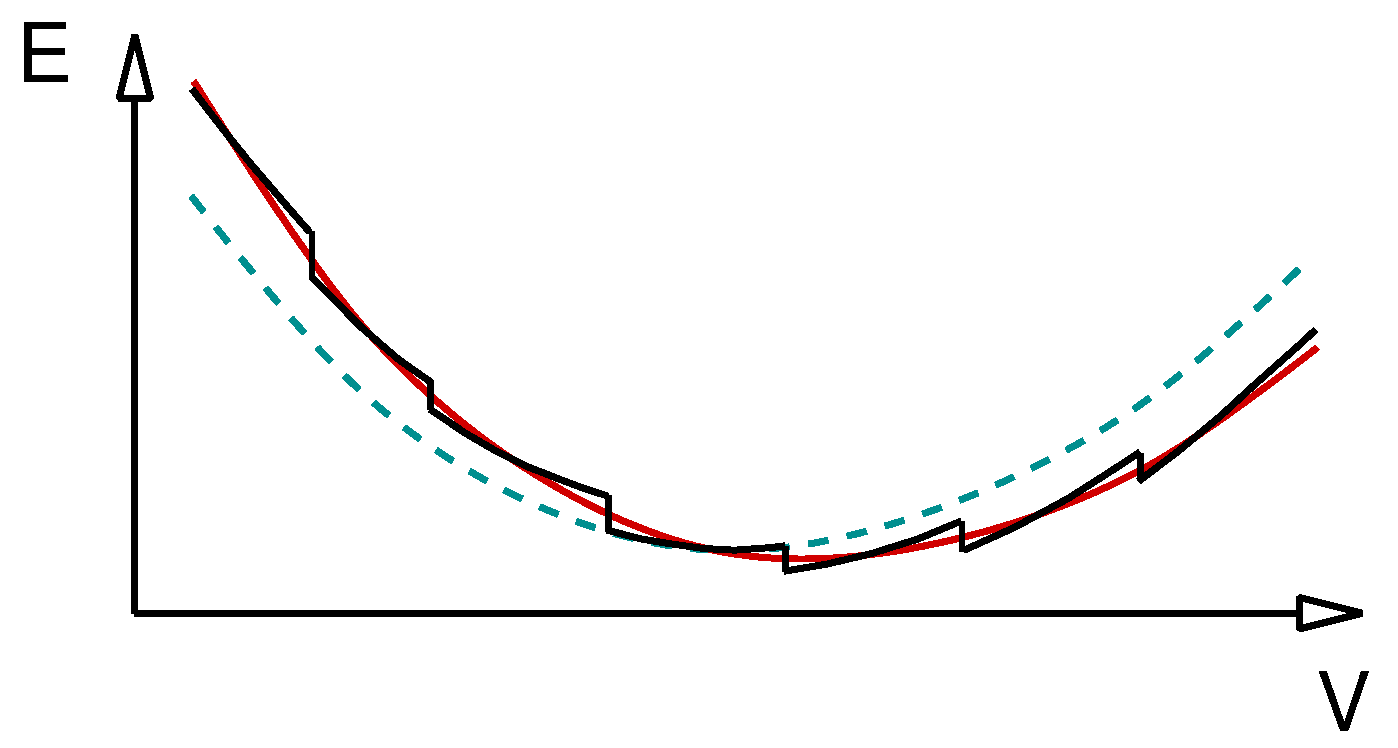
\includegraphics[width=6cm]{Figs/Sawtooth/sawtooth.eps}
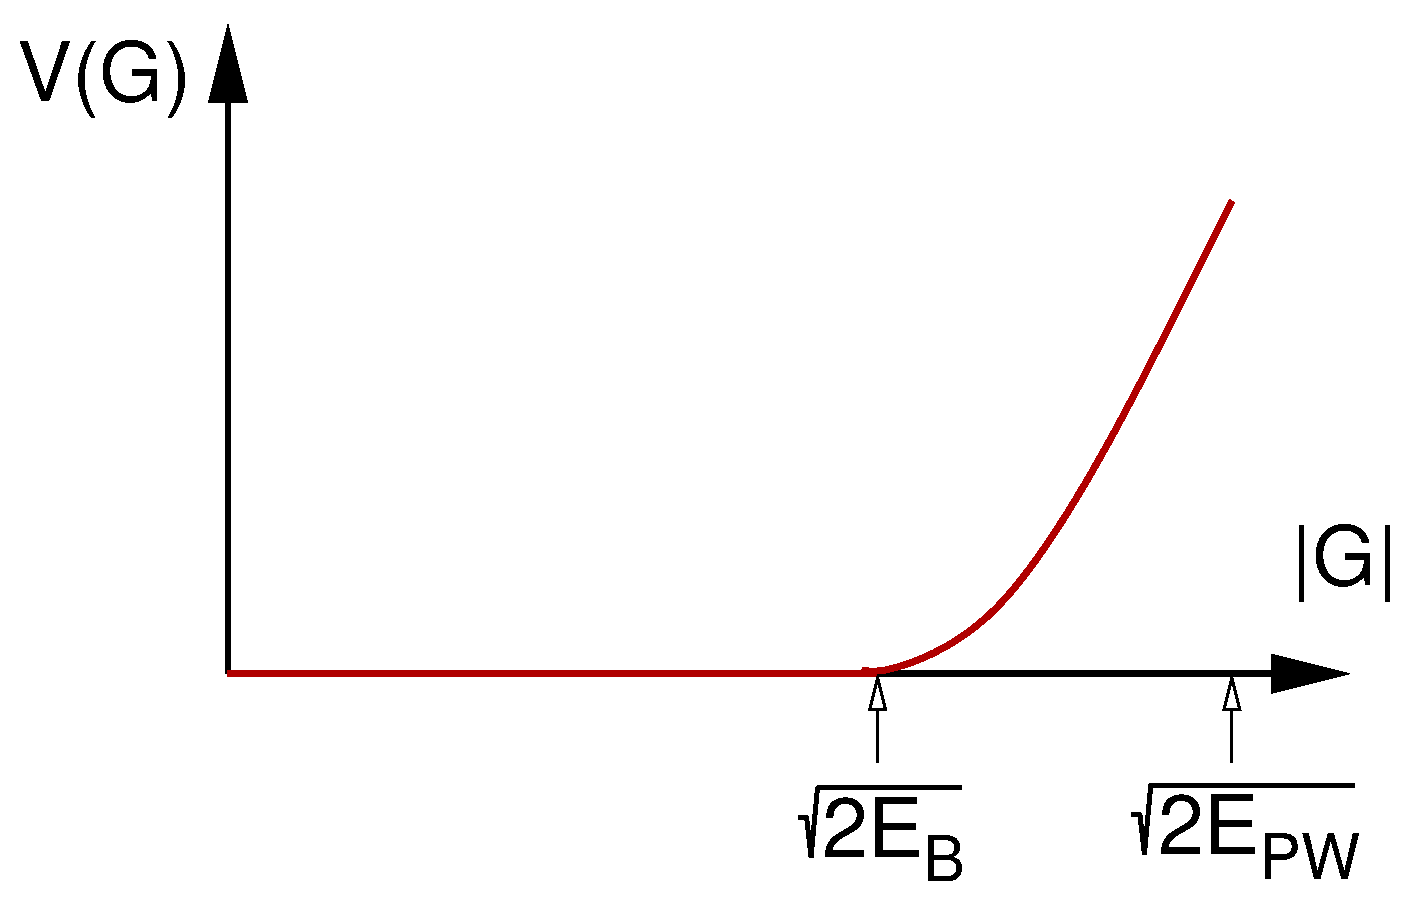
\includegraphics[width=6cm]{Figs/Gbucket/gbucket.eps}
\label{fig:sawtooth}
\caption{Left: Sawtooth behavior of the total energy as function of
volume with a fixed plane wave cutoff (black) with a fixed number of
plane waves (green dashed) and the correct result with a fully
converged calculation (red). By adding a G-dependent potential the
plane wave convergence can be artificially accelerated.}
\end{figure}

The steps in the total energy vanish if the calculation is fully converged in
the basis set size, because additional basis functions do not lower the total
energy. If the function is not converged, the best result is obtained by
keeping the same plane wave cutoff. However, if a the energy obtained at a few
points is then fitted to, for example, a parabola or the Murnaghan equation of
state\cite{murnaghan44_pnas30_244}, one has to be careful with the steps. A
step can considerably mess up the fit. In these cases it is better to use a
larger step size in the lattice constant.

This sawtooth behavior can be suppressed by including an additional
G-dependent bucket potential that ensures that the wave function
coefficients at the plane wave cutoff vanish strictly.

%==========================================================================
\subsection{Overcompleteness problem when using too many projector functions}
%==========================================================================
When testing the convergence with respect to the number of projector
functions one usually runs into instabilities. I believe this problem
is a sort of overcompleteness problem. There is no rigorous
investigation so far.

The problem is the following: One cannot map a number of N projector
functions onto less than N real space grid points. On the grid they
are no more distinguishable. Thus there are combinations of partial
waves with coefficients that are completely decoupled from the plane
wave part. 

To illustrate the problem let us estimate the number of degrees of
freedom on a grid with a given plane wave cutoff in spheres of
different radius $r$.

\begin{center}
\begin{tabular}{|r|r|r|r|}
\hline
r      & 20 Ry & 40 Ry & 60 Ry \\
\hline
1.5 a$_0$ &  5 &  14 &  26 \\
2   a$_0$& 12 &  34 &  62 \\
2.5 a$_0$& 23 &  66 &  122\\
3   a$_0$& 40 & 115 & 211 \\
\hline
\end{tabular}
\end{center}

A semi-core setup with two shells of s- and p-character and, in
addition one shell for d and f electrons yields 20 projector
functions.




%==========================================================================
\subsection{Constraints acting on atoms}
%==========================================================================


%==========================================================================
\subsection{Electrostatic decoupling and coupling of point charges}
%==========================================================================

%==========================================================================
\subsection{Non-collinear densities}
\label{sec:noncollinear}
%==========================================================================
In the current implementation the non-collinear spin density is first
transformed into a locally collinear spin density, from which the
exchange functional is evaluated. 
\begin{eqnarray*}
n_s(\vec{r})= |\vec{\sigma}(\vec{r})|
\end{eqnarray*}

The choice is non-unique regarding gradient corrections because the
gradient of the spin density is a tensor.
\begin{eqnarray*}
\partial_u\sigma_j(\vec{r})
\end{eqnarray*}
Our choice
\begin{eqnarray*}
\vec{\nabla}n_s(\vec{r})=\vec{\nabla}|\vec{\sigma}(\vec{r})|
\end{eqnarray*}
is only one of the possible choices. 


For the one-center densities, we evaluate
\begin{eqnarray*}
n_s&=&\sqrt{Q^2+\left(\vec{\sigma}^2-Q^2\right)}
=Q\sqrt{1+\left(\frac{\vec{\sigma}^2}{Q^2}-1\right)}
\\
&=&Q\Bigl[1+\frac{1}{2}\left(\frac{\vec{\sigma}^2}{Q^2}-1\right)
-\frac{1}{8}\left(\frac{\vec{\sigma}^2}{Q^2}-1\right)^2+\ldots
\end{eqnarray*}
where $Q$ is defined as
\begin{eqnarray*}
Q&=&\sqrt{C+(\hat{P}_s\vec{\sigma})^2}
\end{eqnarray*}
and $\hat{P}_s$ is an operator the projects out nonspherical terms
from the spin density. The constant is a small value that avoids a 
divide-by-zero.

Note, that these approximations are not necessary for collinear
densities. Therefore the results of collinear and non-collinear
densities differ even though the density may be collinear!

There is a second implementation, which is even more approximate, but
it provides the exact result for strictly collinear densities. This
option must be enabled in the code.

%==========================================================================
\subsection{Cell dynamics}
%==========================================================================
%==========================================================================
\subsubsection{Constraints}
\label{sec:unitcellconstraints}
%==========================================================================
Let $\mat{T}(t)$ with
\begin{eqnarray}
\mat{T}=\left(\begin{array}{ccc}
T_{x,1} & T_{x,2} & T_{x,3}\\
T_{y,1} & T_{y,2} & T_{y,3}\\
T_{z,1} & T_{z,2} & T_{z,3}\\
\end{array}\right)
\end{eqnarray}
be the $3\times3$ matrix formed by the lattice vectors
$\vec{T}_1,\vec{T}_2,\vec{T}_3$.  Each constraint is expressed in
terms of a matrix $\mat{C}_\lambda$. 


$\Delta\mathcal{L}$ is the contribution of the constraints to the
Lagrangian using the method of Lagrange multipliers.  The constraints
are labeled by $\lambda$. $\gamma_\lambda$ is the Lagrange
multiplier.
\begin{eqnarray}
    \Delta\mathcal{L}(\mat{T},\dot{\mat{T}})
&=& \sum_\lambda \gamma_\lambda
         \Tr\Bigl[\mat{C}^\dagger_\lambda
                  \bigl(\mat{T}(t)\mat{T}^{-1}_{\text{ref}}-\mat{1}\bigr)
                  \Bigr]
\end{eqnarray}

The resulting force of constraint is
\begin{eqnarray}
-\frac{\delta\Delta\mathcal{L}(\mat{T},\dot{\mat{T}})}{\delta \mat{T}^\dagger}
&=& -\biggl(\mat{T}^{-1}_{\text{ref}}
\Bigl(\sum_\lambda \mat{C}^\dagger_\lambda \gamma_\lambda
                  \Bigr)\biggr)^\dagger
\end{eqnarray}

The Lagrange multipliers are determined so that the constraint is
obeyed along the trajectory. For discrete time steps, the constraint
must be satisfied in the next time step.  Let $\mat{T}(0)$ be the
lattice vectors at the current time step, which we use as the
reference cell $\mat{T}_{\text{ref}}$. Let $\mat{T}(+)$ be the lattice
vectors at the next time step.  $\mat{\bar{T}}$ be the lattice vectors
propagated to the next time step, albeit without constrains.  The
lattice vectors are first propagated without constraints. The lattice
vectors of the next time step also experience the forces of
constraint, so that
\begin{eqnarray}
\mat{T}(+)&=&\mat{\bar{T}}+\sum_{\lambda}x_\lambda\mat{C}_\lambda
\mat{T}^{-1,\dagger}(0)
\end{eqnarray}
Because the Lagrange multipliers carry different factors in the
continuous and the discrete time, we rename then from now on by a
different symbol, namely $\vec{x}$. 

The constraint labeled by $\lambda$ is
\begin{eqnarray}
0&=&\Tr\Bigl[\mat{C}^\dagger_\lambda
                  \Bigl(\mat{T}(+)\mat{T}^{-1}(0)-\mat{1}\Bigr)
                  \Bigr]
\nonumber\\
&=& \Tr\Bigl[\Bigl(\mat{\bar{T}}\mat{T}^{-1}(0)
+\sum_{\lambda'}x_{\lambda'} \mat{C}_{\lambda'}\mat{T}^{-1,\dagger}(0)\mat{T}^{-1}(0)
-\mat{1}\Bigr)\mat{C}^\dagger_\lambda\Bigr]
\nonumber\\
&=& 
\underbrace{
\Tr\Bigl[\Bigl(\mat{\bar{T}}\mat{T}^{-1}(0)
-\mat{1}\Bigr)\mat{C}^\dagger_\lambda\Bigr]}_{b_\lambda}
+\sum_{\lambda'}x_{\lambda'} 
\underbrace{
\Tr\Bigl[
\mat{C}_{\lambda'}\mat{T}^{-1,\dagger}(0)\mat{T}^{-1}(0)
\mat{C}^\dagger_\lambda\Bigr]
}_{A_{\lambda,\lambda'}}
\end{eqnarray}
which is a linear system of equations for the $x_\lambda$.

Hence, we obtain the desired values $x_\lambda$ for from
  \begin{eqnarray}
0&=&\sum_{\lambda'}A_{\lambda,\lambda'}x_{\lambda'}+b_\lambda 
\qquad\Rightarrow\quad \vec{x}=-\mat{A}^{-1}\vec{b}
  \end{eqnarray}
with
  \begin{eqnarray}
    b_\lambda&=&\Tr\Bigl[\bigl(\mat{\bar{T}}\mat{T}(0)^{-1}-\mat{1}\bigr)
                      \mat{C}_\lambda^\dagger\Bigr]
 \nonumber\\
    A_{\lambda,\lambda'}
        &=&\mat{C}_\lambda \mat{T}^{-1,\dagger}(0)\mat{T}^{-1}(0)\mat{C}^\dagger_{\lambda'}
  \end{eqnarray}



%==========================================================================
\subsubsection{Use cases for Constraints on the unit cell}
\label{sec:usecasecellconstr}
%==========================================================================
\begin{itemize}
    \item suppress any shear
\begin{center}
\begin{tabular}{|cccc|}
\hline
$C_1=$&$(0,1,0;$&$ 1,0,0 ;$&$ 0,0,0)$\\
$C_2=$&$(0,0,1;$&$ 0,0,0 ;$&$ 1,0,0)$\\
$C_3=$&$(0,0,0;$&$ 0,0,1 ;$&$ 0,1,0)$\\
\hline
\end{tabular}
\end{center}
%
\item suppress any unit-cell rotation\\
\begin{center}
\begin{tabular}{|cccc|}
\hline
$C_1=$&$(0,1,0;$&$ -1,0,0;$&$ 0,0,0)$\\
$C_2=$&$(0,0,1;$&$ 0,0,0 ;$&$ -1,0,0)$\\
$C_3=$&$(0,0,0;$&$ 0,0,1 ;$&$ 0,-1,0)$\\
\hline
\end{tabular}
\end{center}
Caution! do not constrain rotation of unit cell and
\textit{simultaneously} the rotation of the atoms in the unit cell,
unless you are really shure that this is what you want!
%
\item suppress expansion or contraction along $x$ direction
\begin{center}
\begin{tabular}{|cccc|}
\hline
$C_1=($&$1,0,0;$&$ 0,0,0 ;$&$ 0,0,0)$\\
\hline
\end{tabular}
\end{center}
%
\item suppress expansion or contraction along $y$ direction
\begin{center}
\begin{tabular}{|cccc|}
\hline
$C_1=$&$(0,0,0;$&$ 0,1,0 ;$&$ 0,0,0)$\\
\hline
\end{tabular}
\end{center}
%
\item suppress expansion or contraction in $z$ direction
\begin{center}
\begin{tabular}{|cccc|}
\hline
$C_1=$&$(0,0,0;$&$ 0,0,0 ;$&$ 0,0,1)$\\
\hline
\end{tabular}
\end{center}
%
\end{itemize}

%}{} % end of \ifthenelse

%==========================================================================
\newpage
\section{Troubleshooting}
%==========================================================================

%==========================================================================
\subsection{Errors in the input data}
%==========================================================================

\begin{itemize}
\item A common mistake is to enter data with the wrong data type.
  In this case you will receive a message as follows, which should help
  to locate the problem.
\begin{verbatim}
TYPE INCONSISTENT
VARIABLE ID HAS THE VALUE DT
VARIABLE NTH HAS THE VALUE         1
VARIABLE TYPE EXPECTED HAS THE VALUE R(8)
VARIABLE ACTUAL TYPE HAS THE VALUE I(4)
STOP IN LINKEDLIST_GETGENERIC
\end{verbatim}
The first line says that there is a type mismatch. The last line
says that the problem happened in method of the linkedlist object,
which is also responsible for linked list/tree data structures such as
block-structured input files. In particular the program attempts to
collect a data item from this tree structure.  The second line gives
you the name of the variable, in this example ``DT'', which is the key
word for the time step. It cannot tell in which file or which block
the data is located. The third line tells you that it is the first
data with this name in the block. The next two lines say that the
program expects a data with type ``real(8)'', but finds one of type
``integer(4)''. It appears that the program has mistaken your data for
DT as an integer, because the user forgot to type the decimal point.
\item The program does not do what you want it to. You may have mistyped
  keywords, or mixed up the tree structure. This renders a lot of data
  invisible, and the program uses the default values. Try to consult
  the protocol of the program. It should report all options selected.
  If options are not listed, the option is not selected, or the
  corresponding value is zero. (Of course, it can also be that it is
  not reported. In this case see whether you get a statement in the
  protocol if you select the option. If not, please report this to the
  author.)
\item If you did not provide, or mistype, a keyword that does not have
  a default, you may receive a message like this:
\begin{verbatim}
KEYWORD T= IS MANDATORY
STOP IN STRCIN; !STRUCTURE!LATTICE
\end{verbatim}

\end{itemize}



\subsection{Runtime errors}

This is a list of nontrivial user errors from which the program is not
sufficiently protected and loose ends of the code where particular
caution is needed. It is my goal to adjust the program to
keep this list as short as possible.

\begin{enumerate}
\item Sometimes the program stops with an error message saying 
  ``LOOP FOR ORTHOGONALIZATION NOT CONVERGED''. This is an indication
  of extremely large changes of the wave functions, which can no
  longer be orthogonalized. There are several possible problems that can
  lead to this, and several possible remedies: 
  \begin{itemize}
  \item The atomic positions have been chosen with unreasonably short
    distances, or with atoms lying on top of each other.
  \item Some setups produce this behavior in the first few time steps.
    In this case reduce the plane wave cutoff to a small value such as
    5, 10 or 20 Ry. If this alone does not help, also reduce the time
    step, but leave the wave function masses MPSI and MPSICG2
    constant. It is sufficient to do this for the first few (about five
    or ten) time steps. If you started a new job with gradient
    corrected DFT functionals, you should try
    ``!CONTROL!FOURIER:CDUAL=4'' or reach convergence first for a
    truly local functional before switching gradient corrections
    on. If the kinetic energy for the wave functions decreases to a
    reasonable value of a few Hartree, one can restart with the
    original values.
  \item If all this does not help, you are in trouble!
  \end{itemize}
\item If the program produces a coredump, increase first the stack size
  using the ``ulimit'' command. You can also control the size of the stack
  array using the compiler option -bmaxstack.
\item The code has a limited size of the send-receive buffer. The
  program is not guarded against a buffer overflow, even though the MPI
  Library should give a useful message (affects only the parallel
  version).
\item Errors occur if the operating system, Fortran runtime
  environment or SP2 Software are not on the same level, 
  used during compilation.
\item If you find that the program crashes without providing an error
  message, and if you have the source code, specify
  \verb|!CONTROL!GENERIC:TRACE=T|. The program will then
  continuously write information on subroutines entered and left,
  which often allows one to locate the problem. Note that, in order to
  avoid producing files that are too large to be useful, not all routines
  result in a trace message.  \ifthenelse{\boolean{private}}{
\item The routine "MADELUNG" chooses itself the range of real and
    reciprocal space summations. It has not been sufficiently tested
    whether these choices are accurate. It may affect the result of
    the object "Isolate" that separates isolated molecules from its
    periodic images.
\item The Becke88 gradient correction\cite{becke88_pra38_3098}for exchange
  produces unreasonable results if the total density or the spin density is
  vanishes. In this case small numerical values for the gradient pick up a
  singularity in the functional form. This may happen for a fully spin
  polarized system. The cure is to pick another density functional, which does
  not contain the Becke88 functional.
}{} %end of ifthenelse
\end{enumerate}


%==========================================================================
\subsection{Overcompleteness of projector functions}
%==========================================================================
Using too many partial waves leads to so-called
\textbf{overcompleteness}\index{overcompleteness} of projector
functions.  This is counterintuitive because one would think that more
terms would make the description more accurate. 

The origin of the problem is that, with a finite plane wave cutoff,
the wave function has only a limited number of degrees of freedom
inside the atomic region. If the number of projector functions
exceeds this number of degrees of freedom, there is at least one
partial wave with a prefactor that is not fixed by the wave function.
If this partial wave increases the energy, it will be projected
out. If it, however, lowers the energy the calculation becomes
unstable and the results unphysical.

\begin{eqnarray}
N&=&\frac{4\pi}{3}G_x^3\frac{1}{V_G}
\stackrel{V_G=(2\pi)^3/V_R}{=}
\frac{4\pi}{3}G_x^3\frac{V_R}{(2\pi)^3}
\nonumber\\
&\stackrel{E_{PW}=\frac{1}{2}G_x^2}{=}&
\frac{4\pi}{3}\Bigl(2 E_{PW}\Bigr)^\frac{3}{2}\frac{V_R}{(2\pi)^3}
\nonumber\\
\Rightarrow\qquad
\frac{N}{V_R}&=&\frac{4\pi}{3}\Bigl(
\frac{\sqrt{2E_{PW}}}{2\pi}
\Bigr)^3
\nonumber\\
\sum_{\ell=0}(2\ell+1)n_\ell&<&
\frac{4\pi}{3}r_{cov}^3\frac{4\pi}{3}\Bigl(
\frac{\sqrt{2E_{PW}}}{2\pi}
\Bigr)^3
=\underbrace{\frac{2}{9\pi}}_{\approx 1/30}\Bigl(r_{cov}\sqrt{2E_{PW}}\Bigr)^3
\end{eqnarray}
Here $N$ is the number of plane waves, or the number of real-space
grid points respectively. $n_\ell$ is the number of different radial
partial waves for the main angular momentum $\ell$.  $G_x$ is the
maximum size for the wave vectors considered. $V_R$ is the real-space
unit-cell volume. $V_G$ is the reciprocal-space unit-cell
volume. $E_{PW}=\frac{1}{2}G_x^2$ is the plane wave cutoff and
$r_{cov}$ is the covalent radius.


We obtain
\begin{center}
\begin{tabular}{|c|c|c|c|c|}
\hline
  &$r_{cov}$ & 20~Ry & 30~Ry & 50~Ry\\
\hline
H & 0.32~\AA &  1.4 & 2.5  &  5.5\\
O & 0.73~\AA & 16.6 & 30.5 & 65.6\\ 
Si& 1.11~\AA & 58.4 & 107.2 & 230.8\\
\hline
\end{tabular}
\end{center}
On the right-hand side the estimated number of degrees of freedom are
listed. It should be considered that the effective augmentation radius
is usually smaller than the covalent radius. This ratio enters to the
third power. Hence, if the augmentation radius is 20~\% smaller than
the covalent radius only half the number of degrees of freedom are
present.

This table indicates that for hydrogen, only the s-type projector
should be used. For second-row elements the choice of the number of
projectors appears fairly uncritical. For first-row elements, however,
instabilities may already be present if only one projector function
is used for s, p, and d-type angular momenta.


%==========================================================================
\newpage
\section{Code documentation}
%==========================================================================
%==========================================================================
\subsection{Strategy}
%==========================================================================
The main documentation for the user is the manual file. It shall
contain a complete description of all input parameters and their
functionality.

For the algorithms we prepare reports with a detailed description and
their theoretical background. These reports are currently only for
internal use. 

The code is written as self-explanatory as possible. I understand that
this looks like an excuse for not documenting the code. The idea
behind is to use meaningful variable names, use explicit typing such
as declaring each variable explicitly, declaring its intent
(in,out,inout), and to use similar structures and conventions
throughout the code. This technique avoids the common problem that
documentation and code become asynchronous.

%==========================================================================
\subsection{Doxygen}
%==========================================================================
Doxygen is a tool for code analysis and automatic code
documentation. It is a free multi-platform tool available at
\url{http://www.stack.nl/~dimitri/doxygen/}. Most useful are the call
graphs and caller graphs, which provide a quick overview of the code
structure.

The CP-PAW code supports analysis with Doxygen. Currently this is in a
testing phase and not in its final implementation. 

On OSX, I installed doxygen with the option \verb|with-graphviz| in
order to be able to prepare call graphs and caller graphs. 
\begin{verbatim} 
brew install doxygen --with-graphviz
\end{verbatim}
The graph-drawing kit graphviz can be obtained from
\url{http://www.graphviz.org/}.

\begin{itemize}
\item Only the debug version of the code is analyzed. Therefore, the
  debug version must be compiled with \verb|make dbg| before analyzing
  it with doxygen. 
%
\item \verb|make doxygen| constructs a configuration file ``Doxyfile''
  and it generates from it the doxygen information.  The information
  generated is held in directory \verb|Doxydocs| in the directory
  which holds the paw executables.
%
\item The data are represented as a net of interlinked web-pages.
on MacOS one can view the data with
\begin{verbatim}
A=$(which paw_dbg.x)
open ${A%paw_dbg.x}Doxydocs/html/index.html
\end{verbatim}
On other operating systems, the file can be accessed with any
web-browser instead of \verb|open|.

First, the variable $A$ is defined as the filename of
\verb|paw\_dbg.x| with the full path. With \verb|${A%paw_dbg.x}|, we
obtain the path without the trailing file name, which allows us to
build up the full filename of the main web site holding the doxygen
data. This \verb|index.html| file is then opened with a web browser.
%
\end{itemize}


Remark: A box in the call graph with red borders indicates that the
node has more arrows than shown.


\appendix
%==========================================================================
\section{Installation}
%==========================================================================
The CP-PAW code package is publicly available under at
\begin{verbatim}
https://github.com/cp-paw/cp-paw
\end{verbatim}

Place the distribution into some directory, which I will call in the
following your base-directory of the cppaw distribution. In this
distribution you should see the following with \verb|ls|.
\begin{verbatim}
LICENSE paw_install README src 
\end{verbatim}


%==========================================================================
\subsection{Automatic installation: Try your luck}
%==========================================================================
Ideally, the cppaw-package installs itself when one executes
\begin{verbatim}
./paw_install
\end{verbatim}
on the command line from within the base directory of the cppaw
distribution.

The command relies on defaults collected in a parameter file. The
parmfile actively explores the environment, it runs on, and choses a
suitable set of parameters. Because building up the underlying
knowlegde base is an ongoing process, one should also be prepared that
the automatic installation fails. In that case, the parameters
parmfile can be set by hand as sketched in the next section entitled
``Adjust the parameter file''.

If you have been lucky and the install command above worked, test the
success with the following commands.
\begin{verbatim}
ls bin/fast_parallel/ppaw_fast
ls bin/fast/paw_fast
ls bin/fast/paw_strc
ls bin/fast/libpaw.a
ls doc/manual.pdf
\end{verbatim}
If none of the commands complains ``No such file or directory''. The
installation is probably ok. 


The directory structure will have the following form
\begin{center}
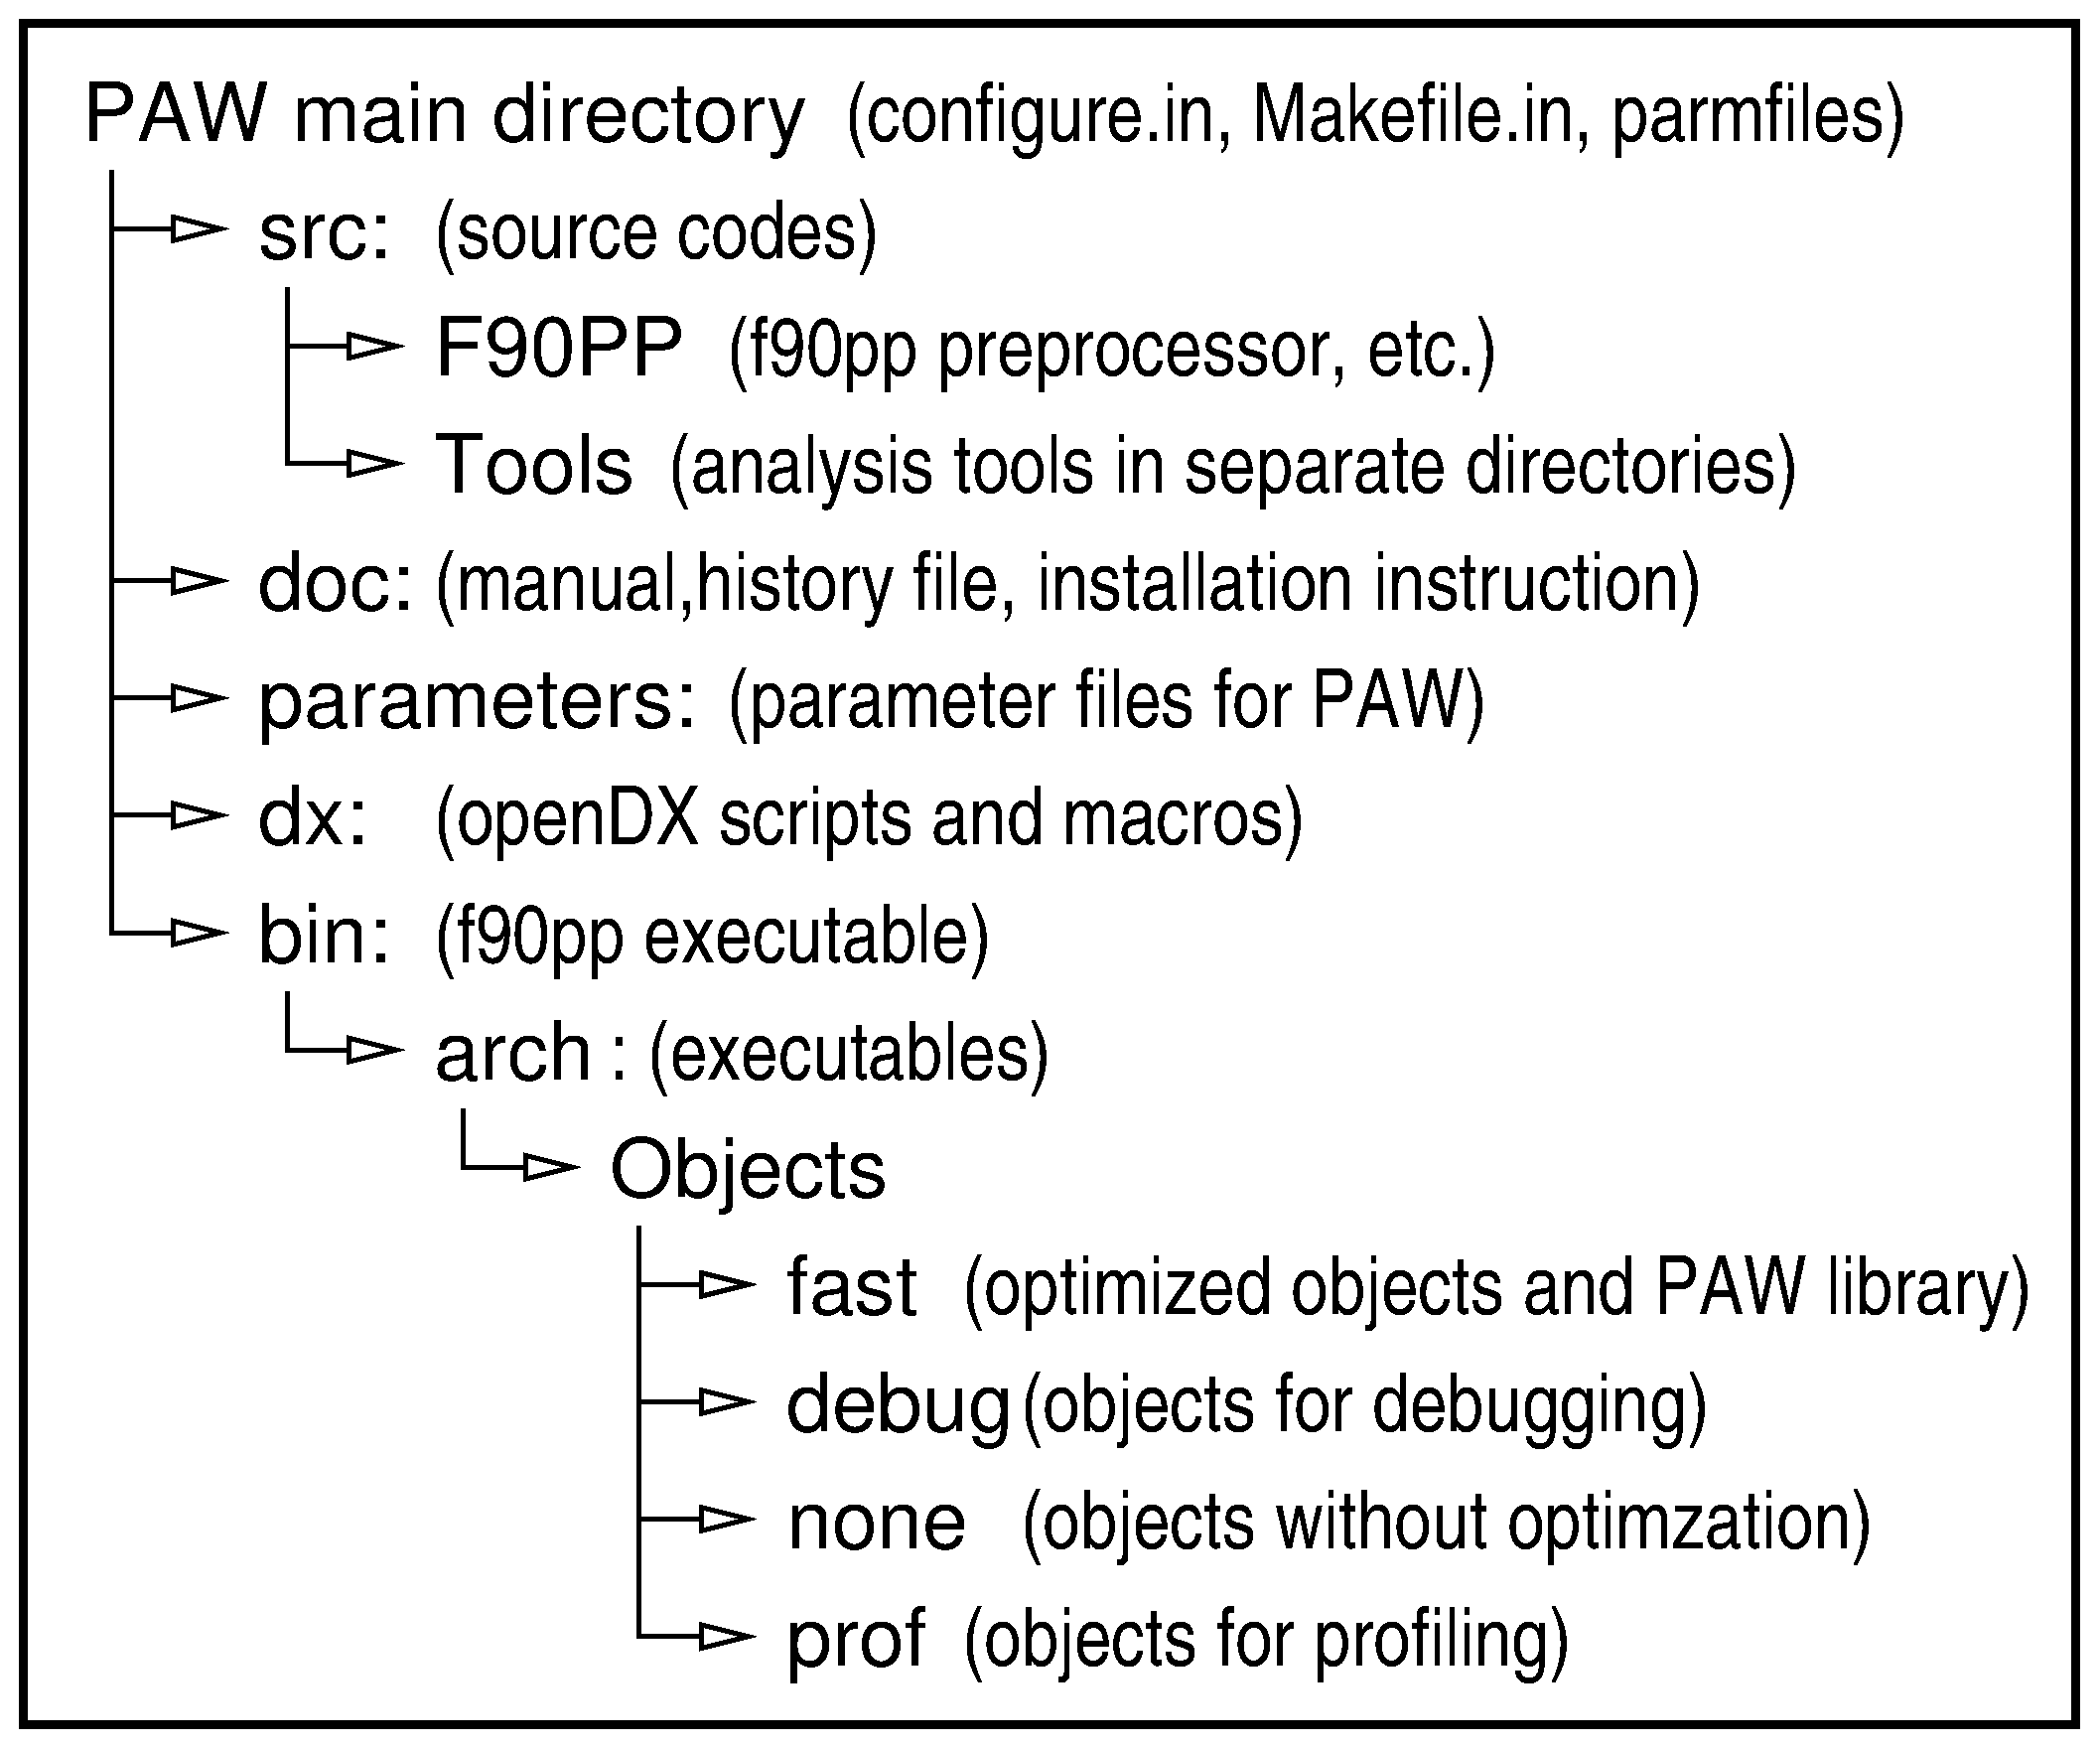
\includegraphics[width=0.8\linewidth]{Figs/PAWdirtree/pawdirtree.eps}
\end{center}

Finally, open the manual \verb|doc/manual.pdf| to find further
information.

%==========================================================================
\subsection{Adjust the parameter file}
%==========================================================================
If the installation with the current defaults did not work, you need
to adjust the parameter file. First,  make a copy of
current default parameter file, for example in the base directory. (I
assume that this is still your current directory.)
\begin{verbatim}
cp src/Buildtools/defaultsparmfile ./parmfile
\end{verbatim}

The parameter file is a bash script, which defines a set of parameters
required for the installation. The parameters are briefly explained in
the top section of the parameter file. After you adjuste the
parameters to your needs, you try the installation again, but now with
your own parameter file (e.g. \verb|my_fast|) and probably with your own
selection.
\begin{verbatim}
src/Buildtools/paw_build.sh -c my_fast -f parmfile
\end{verbatim}

This is the point, from which you either know how to proceed, or you
need to ask for help. This is why I do not elaborate on the
installation at this point.

%==========================================================================
\subsection{Version control}
%==========================================================================
The CPPAW package is under version control under GIT. There are
mechanisms to identify the instance that has been compiled into the
code used to produce results. The relevant information is printed in
the protocol, the main output file, of the simulation code.

The simulation code comes in different flavors, such as
\verb|paw_dbg.x|, \verb|paw_fast.x|. The corresponding parallel
version which begin with a double ``p'' for ``parallel paw'', such as
in \verb|ppaw_fast.x|.

%==========================================================================
\subsection{Version information}
%==========================================================================
The version information of a simulation code can be extracted
with\footnote{Another possibility is to use the tool
\texttt{\${PAWDIR}/src/Buildtools/Version/myversion.sh}}
\begin{verbatim}
paw_fast.x -v
\end{verbatim}
The information should be sufficient to identify the exact version in
the git repository.


%==========================================================================
\subsection{Source blob}
%==========================================================================
A complete copy of the source code is contained in each executable of
the simulation code. It is called the \textbf{source~blob}
\index{source~blob}.

The source blob can be extracted, for example, by\footnote{The shell
script is located at \texttt{src/Tools/Scripts/paw\_getsrc.sh} in the
repository and will be copied into the \texttt{bin}-directory during
installation using \texttt{make scripts}}
\begin{verbatim}
paw_getsrc.sh -x paw_fast.x -o paw_src.tgz
\end{verbatim}
where \verb|paw_fast.x| is the executable from which the source blob
shall be extracted and \verb|paw_src.tgz| is the resulting compressed
tar file with the source blob.


\newpage
%====================================================================
\section{Symmetry tables}\label{section:symmetry_tables}
%====================================================================
%====================================================================
\subsection{Bravais lattices}
%====================================================================
Unit cells definitions by Bradley and Cracknell\cite{bradley72_book}:
\begin{center}
\begin{tabular}{|c|c|c|c|c|}
\hline
\multicolumn{2}{|c|}{Bravais Lattice} & $\vec{T}_1$& $\vec{T}_2$& $\vec{T}_3$\\
\hline
\hline
\multicolumn{5}{|c|}{triclinic}\\
\hline
primitive & $\Gamma_1$ & & &\\
\hline
%
\hline
\multicolumn{5}{|c|}{monoclinic}\\
\hline
primitive & $\Gamma_m$ & 
$(0,-b,0)$ & 
$(a\sin(\gamma),-a\cos(\gamma),0)$ 
&$(0,0,c)$ \\
base centered & $\Gamma_m^b$ & 
$(0,-b,0)$ & 
$\frac{1}{2}(a\sin(\gamma),-a\cos(\gamma),-c)$ &
$\frac{1}{2}(a\sin(\gamma),-a\cos(\gamma),c)$ \\
\hline
%
\hline
\hline
\multicolumn{5}{|c|}{orthorhombic}\\
\hline
primitive & $\Gamma_o$ & 
$(0,-b,0)$ & 
$(a,0,0)$ 
&$(0,0,c)$ \\
base centered & $\Gamma_o^b$ & 
$(\frac{1}{2}a,-\frac{1}{2}b,0)$ & 
$(\frac{1}{2}a,\frac{1}{2}b,0)$ & 
$(0,0,c)$ \\
body centered & $\Gamma_o^v$ & 
$\frac{1}{2}(a,b,c)$ & 
$\frac{1}{2}(-a,-b,c)$ & 
$\frac{1}{2}(a,-b,-c)$ \\
face centered & $\Gamma_o^f$ & 
$\frac{1}{2}(a,0,c)$ & 
$\frac{1}{2}(0,-b,c)$ & 
$\frac{1}{2}(a,-b,0)$ \\
\hline
%
\hline
\multicolumn{5}{|c|}{tetragonal}\\
\hline
primitive & $\Gamma_q$ & 
$(a,0,0)$ & 
$(0,a,0)$ 
&$(0,0,c)$ \\
\hline
body centered &$\Gamma_q^v$ & 
$\frac{1}{2}(-a,a,c)$ & 
$\frac{1}{2}(a,-a,c)$ & 
$\frac{1}{2}(a,a,-c)$ \\
\hline
%
\hline
\multicolumn{5}{|c|}{trigonal}\\
\hline
primitive & $\Gamma_{rh}$ & 
$(0,a,c)$ & 
$(\frac{1}{2}\sqrt{3}a,\frac{1}{2}a,c)$ &
$(-\frac{1}{2}\sqrt{3}a,\frac{1}{2}a,c)$ \\
\hline
%
\hline
\multicolumn{5}{|c|}{hexagonal}\\
\hline
primitive & $\Gamma_h$ & 
$(0,-1,0)a$ & 
$(\frac{1}{2}\sqrt{3},\frac{1}{2},0)a$ &
$(0,0,1)c$\\
\hline
%
\hline
\multicolumn{5}{|c|}{cubic}\\
\hline
primitive & $\Gamma_c$ & 
$(1,0,0)a$ & 
$(0,1,0)a$ & 
$(0,0,1)a$ \\
face centered & $\Gamma_c^f$ & 
$\frac{1}{2}a(0,1,1)$ & 
$\frac{1}{2}a(1,0,1)$ & 
$\frac{1}{2}a(1,1,0)$ \\
body centered & $\Gamma_c^v$ & 
$\frac{1}{2}a(-1,1,1)$ & 
$\frac{1}{2}a(1,-1,1)$ & 
$\frac{1}{2}a(1,1,-1)$ \\
\hline
\end{tabular}
\end{center}

%====================================================================
\newpage
\subsection{Spacegroups}
%====================================================================
The translation between the spacegroup number and the international
space group symbols is given in tables~\ref{table:spacegroupnumber_a}
and \ref{table:spacegroupnumber_b}.
\begin{table}[h!]
\begin{center}
\begin{tabular}{||r|l||r|l||r|l||r|l||r|l||}
\hline
1      & P1                 & 
2      & P$\bar{1}$         & 
3      & P2                 & 
4      & P2$_1$             & 
5      & C2                 \\
6      & Pm                 & 
7      & Pc                 & 
8      & Cm                 & 
9      & Cc                 & 
10     & P2/m               \\
11     & P2$_1$/m           & 
12     & C2/m               & 
13     & P2/c               & 
14     & P2$_1$/c           & 
15     & C2/c               \\
16     & P222               & 
17     & P222$_1$           & 
18     & P2$_1$2$_1$2       & 
19     & P2$_1$2$_1$2$_1$   & 
20     & C222$_1$           \\
21     & C222               & 
22     & F222               & 
23     & I222               & 
24     & I2$_1$2$_1$2$_1$   & 
25     & Pmm2               \\
26     & Pmc2$_1$           & 
27     & Pcc2               & 
28     & Pma2               & 
29     & Pca2$_1$           & 
30     & Pnc2               \\
31     & Pmn2$_1$           & 
32     & Pba2               & 
33     & Pna2$_1$           & 
34     & Pnn2               & 
35     & Cmm2               \\
36     & Cmc2$_1$           & 
37     & Ccc2               & 
38     & Amm2               & 
39     & Aem2               & 
40     & Ama2               \\
41     & Aea2               & 
42     & Fmm2               & 
43     & Fdd2               & 
44     & Imm2               & 
45     & Iba2               \\
46     & Ima2               & 
47     & Pmmm               & 
48     & Pnnn               & 
49     & Pccm               & 
50     & Pban               \\
51     & Pmma               & 
52     & Pnna               & 
53     & Pmna               & 
54     & Pcca               & 
55     & Pbam               \\
56     & Pccn               & 
57     & Pbcm               & 
58     & Pnnm               & 
59     & Pmmn               & 
60     & Pbcn               \\
61     & Pbca               & 
62     & Pnma               & 
63     & Cmcm               & 
64     & Cmce               & 
65     & Cmmm               \\
66     & Cccm               & 
67     & Cmme               & 
68     & Ccce               & 
69     & Fmmm               & 
70     & Fddd               \\
71     & Immm               & 
72     & Ibam               & 
73     & Ibca               & 
74     & Imma               & 
75     & P4                 \\
76     & P4$_1$             & 
77     & P4$_2$             & 
78     & P4$_3$             & 
79     & I4                 & 
80     & I4$_1$             \\
81     & P$\bar{4}$                & 
82     & I$\bar{4}$                & 
83     & P4/m               & 
84     & P4$_2$/m           & 
85     & P4/n               \\
86     & P4$_2$/n           & 
87     & I4/m               & 
88     & I4$_1$/a           & 
89     & P422               & 
90     & P42$_1$2           \\
91     & P4$_1$22           & 
92     & P4$_1$2$_1$2       & 
93     & P4$_2$22           & 
94     & P4$_2$2$_1$2       & 
95     & P4$_3$22           \\
96     & P4$_3$2$_1$2       & 
97     & I422               & 
98     & I4$_1$22           & 
99     & P4mm               & 
100    & P4bm               \\
101    & P4$_2$cm           & 
102    & P4$_2$nm           & 
103    & P4cc               & 
104    & P4nc               & 
105    & P4$_2$mc           \\
106    & P4$_2$bc           & 
107    & I4mm               & 
108    & I4cm               & 
109    & I4$_1$md           & 
110    & I4$_1$cd           \\
111    & P$\bar{4}$2m              & 
112    & P$\bar{4}$2c              & 
113    & P$\bar{4}$2$_1$m          & 
114    & P$\bar{4}$2$_1$c          & 
115    & P$\bar{4}$m2              \\
116    & P$\bar{4}$c2              & 
117    & P$\bar{4}$b2              & 
118    & P$\bar{4}$n2              & 
119    & I$\bar{4}$m2              & 
120    & I$\bar{4}$c2              \\
\hline
\end{tabular}
\end{center}
\caption{\label{table:spacegroupnumber_a}Space group number as given
  in the ``International tables for Crystallography, Vol. A'' and the
  corresponding international space group symbol (Herman-Maughin
  notation). Retrieved from the Bilbao Crystallographic Server
  \url{http://www.cryst.ehu.es/cryst/text/table.html} on Dec. 21,
  2013.  For further information, see Aroyo, et. al. Zeitschrift f\"ur
  Kristallographie (2006), 221, 1, 15-27.  }
\end{table}


\begin{table}[!h]
\begin{center}
\begin{tabular}{||r|l||r|l||r|l||r|l||r|l||}
\hline
121    & I$\bar{4}$2m              & 
122    & I$\bar{4}$2d              & 
123    & P4/mmm             & 
124    & P4/mcc             & 
125    & P4/nbm             \\
126    & P4/nnc             & 
127    & P4/mbm             & 
128    & P4/mnc             & 
129    & P4/nmm             & 
130    & P4/ncc             \\
131    & P4$_2$/mmc         & 
132    & P4$_2$/mcm         & 
133    & P4$_2$/nbc         & 
134    & P4$_2$/nnm         & 
135    & P4$_2$/mbc         \\
136    & P4$_2$/mnm         & 
137    & P4$_2$/nmc         & 
138    & P4$_2$/ncm         & 
139    & I4/mmm             & 
140    & I4/mcm             \\
141    & I4$_1$/amd         & 
142    & I4$_1$/acd         & 
143    & P3                 & 
144    & P3$_1$             & 
145    & P3$_2$             \\
146    & R3                 & 
147    & P$\bar{3}$         & 
148    & R$\bar{3}$         & 
149    & P312               & 
150    & P321               \\
151    & P3$_1$12           & 
152    & P3$_1$21           & 
153    & P3$_2$12           & 
154    & P3$_2$21           & 
155    & R32                \\
156    & P3m1               & 
157    & P31m               & 
158    & P3c1               & 
159    & P31c               & 
160    & R3m                \\
161    & R3c                & 
162    & P$\bar{3}$1m       & 
163    & P$\bar{3}$1c       & 
164    & P$\bar{3}$m1       & 
165    & P$\bar{3}$c1       \\
166    & R$\bar{3}$m        & 
167    & R$\bar{3}$c        & 
168    & P6                 & 
169    & P6$_1$             & 
170    & P6$_5$             \\
171    & P6$_2$             & 
172    & P6$_4$             & 
173    & P6$_3$             & 
174    & P$\bar{6}$                & 
175    & P6/m               \\
176    & P6$_3$/m           & 
177    & P622               & 
178    & P6$_1$22           & 
179    & P6$_5$22           & 
180    & P6$_2$22           \\
181    & P6$_4$22           & 
182    & P6$_3$22           & 
183    & P6mm               & 
184    & P6cc               & 
185    & P6$_3$cm           \\
186    & P6$_3$mc           & 
187    & P$\bar{6}$m2       & 
188    & P$\bar{6}$c2       & 
189    & P$\bar{6}$2m       & 
190    & P$\bar{6}$2c       \\
191    & P6/mmm             & 
192    & P6/mcc             & 
193    & P6$_3$/mcm         & 
194    & P6$_3$/mmc         & 
195    & P23                \\
196    & F23                & 
197    & I23                & 
198    & P2$_1$3            & 
199    & I2$_1$3            & 
200    & Pm$\bar{3}$        \\
201    & Pn$\bar{3}$        & 
202    & Fm$\bar{3}$        & 
203    & Fd$\bar{3}$        & 
204    & Im$\bar{3}$        & 
205    & Pa$\bar{3}$        \\
206    & Ia$\bar{3}$        & 
207    & P432               & 
208    & P4$_2$32           & 
209    & F432               & 
210    & F4$_1$32           \\
211    & I432               & 
212    & P4$_3$32           & 
213    & P4$_1$32           & 
214    & I4$_1$32           & 
215    & P$\bar{4}$3m       \\
216    & F$\bar{4}$3m       & 
217    & I$\bar{4}$3m       & 
218    & P$\bar{4}$3n       & 
219    & F$\bar{4}$3c       & 
220    & I$\bar{4}$3d       \\
221    & Pm$\bar{3}$m       & 
222    & Pn$\bar{3}$n       & 
223    & Pm$\bar{3}$n       & 
224    & Pn$\bar{3}$m       & 
225    & Fm$\bar{3}$m       \\
226    & Fm$\bar{3}$c       & 
227    & Fd$\bar{3}$m       & 
228    & Fd$\bar{3}$c       & 
229    & Im$\bar{3}$m       & 
230    & Ia$\bar{3}$d       \\
\hline
\end{tabular}
\end{center}
\caption{\label{table:spacegroupnumber_b}Space group number as given
  in the ``International tables for Crystallography, Vol. A'' and the
  corresponding international space group symbol (Herman-Maughin
  notation). Retrieved from the Bilbao Crystallographic Server
  \url{http://www.cryst.ehu.es/cryst/text/table.html} on Dec. 21,
  2013.  For further information, see Aroyo, et. al. Zeitschrift f\"ur
  Kristallographie (2006), 221, 1, 15-27.  }
\end{table}


%====================================================================
\newpage
\section{Bands}
%====================================================================
Here I will list the high-symmetry points of the Brillouin zone, for
use with the \verb|paw_bands.x| tool. If the real space lattice vectors are
chosen consistent with the convention below, one can directly use the
relative coordinates as \verb|xk1| and \verb|xk2| in the \verb|bcntl|
file.

See \url{http://lampx.tugraz.at/~hadley/ss1/bzones/}

%====================================================================
\subsection{Face-centered cubic lattice}
%====================================================================
\begin{center}
\renewcommand\arraystretch{1.5}
\begin{tabular}{||c|c||c|c||}
\hline
\multicolumn{2}{|c|}{real space vectors} &
\multicolumn{2}{|c|}{reciprocal space vectors} \\
\hline
$\vec{T}_1$ & $(0,\frac{1}{2},\frac{1}{2}) a$ &
$\vec{g}_1$ & $(-1,1,1)\frac{2\pi}{a}$ \\
$\vec{T}_2$ & $(\frac{1}{2},0,\frac{1}{2}) a$ &
$\vec{g}_2$ & $(1,-1,1)\frac{2\pi}{a}$ \\
$\vec{T}_3$ & $(\frac{1}{2},\frac{1}{2},0) a$ &
$\vec{g}_3$ & $(1,1,-1)\frac{2\pi}{a}$ \\
\hline
\end{tabular}
\renewcommand\arraystretch{1.}
\end{center}

\begin{center}
\renewcommand\arraystretch{1.5}
\begin{tabular}{|c|c|c|}
\hline
\multicolumn{3}{|c|}{$\Gamma-X-W-L-\Gamma-K-X'$}\\
\multicolumn{3}{|c|}{$(0)-(1)-(\frac{3}{2})-(2.20711)-(3.07313)-(4.13379)-(4.48735)$}\\
\hline
Symbol & absolute coord. & relative coord. \texttt{xk1,xk2}\\
\hline
$\Gamma$   & $(0,0,0) \frac{2\pi}{a}$ & $(0,0,0)$ \\ 
$X$        & $(1,0,0) \frac{2\pi}{a}$ & $(0,\frac{1}{2},\frac{1}{2})$ \\ 
$W$        & $(1,\frac{1}{2},0) \frac{2\pi}{a}$ & $(\frac{1}{4},\frac{1}{2},\frac{3}{4})$ \\ 
$L$        & $(\frac{1}{2},\frac{1}{2},\frac{1}{2}) \frac{2\pi}{a}$ & $(\frac{1}{2},\frac{1}{2},\frac{1}{2})$ \\ 
$\Gamma$   & $(0,0,0) \frac{2\pi}{a}$ & $(0,0,0)$ \\ 
$K$        & $(\frac{3}{4},\frac{3}{4},0) \frac{2\pi}{a}$ & $(\frac{3}{8},\frac{3}{8},\frac{3}{4})$ \\ 
$X'$       & $(1,1,0) \frac{2\pi}{a}$ & $(\frac{1}{2},\frac{1}{2},1)$ \\ 
\hline
\end{tabular}
\renewcommand\arraystretch{1.}
\end{center}
The point $K$ lies on the connection from $\Gamma$ to $X'$, where $X'$
is the $X$-point of a nearest neighbor reciprocal lattice vector of the
$\Gamma$ point.

%====================================================================
\subsection{Body-centered cubic lattice}
%====================================================================
\begin{center}
\renewcommand\arraystretch{1.5}
\begin{tabular}{||c|c||c|c||}
\hline
\multicolumn{2}{|c|}{real space vectors} &
\multicolumn{2}{|c|}{reciprocal space vectors} \\
\hline
$\vec{T}_1$ & $(-\frac{1}{2},\frac{1}{2},\frac{1}{2}) a$ &
$\vec{g}_1$ & $(0,1,1)\frac{2\pi}{a}$ \\
$\vec{T}_2$ & $(\frac{1}{2},-\frac{1}{2},\frac{1}{2}) a$ &
$\vec{g}_2$ & $(1,0,1)\frac{2\pi}{a}$ \\
$\vec{T}_3$ & $(\frac{1}{2},\frac{1}{2},-\frac{1}{2}) a$ &
$\vec{g}_3$ & $(1,1,0)\frac{2\pi}{a}$ \\
\hline
\end{tabular}
\renewcommand\arraystretch{1.}
\end{center}

\begin{center}
\renewcommand\arraystretch{1.5}
\begin{tabular}{|c|c|c|}
\hline
\multicolumn{3}{|c|}{$N-\Gamma-H-N-P-\Gamma$}\\
\multicolumn{3}{|c|}{$(0)-(0.7071)-(1.7071)-(2.5731)-(3.0731)-(3.9392)$}\\
\hline
Symbol & absolute coord. & relative coord. \texttt{xk1,xk2}\\
\hline
$\Gamma$   & $(0,0,0) \frac{2\pi}{a}$ & $(0,0,0)$ \\ 
$H$        & $(1,0,0) \frac{2\pi}{a}$ & $(-\frac{1}{2},\frac{1}{2},\frac{1}{2})$ \\ 
$P$        & $(\frac{1}{2},\frac{1}{2},\frac{1}{2}) \frac{2\pi}{a}$ & $(\frac{1}{4},\frac{1}{4},\frac{1}{4})$ \\ 
$N$        & $(\frac{1}{2},\frac{1}{2},0) \frac{2\pi}{a}$ & $(0,0,\frac{1}{2})$ \\ 
\hline
\end{tabular}
\renewcommand\arraystretch{1.}
\end{center}
\clearpage


%====================================================================
\newpage
\section{Density functionals and their identifiers in LibXC}
\label{sec:libxcids}
%====================================================================
In tables \ref{tab:libxc1}, the identifiers for the density
functionals in the library LibXC are listed. They are taken from the
file \verb|src/libxc_inc.f90| beginning of 2024. Only a small fraction
is currently made available, but this shall change soon.


\begin{table}[hbt]
\caption{\label{tab:libxc1}Density Functionals and their identifiers
  in LibXC. Part~1}
\begin{center}
\begin{tabular}{llr}
\hline
\hline
Description & ID & index\\
\hline
  'Slater exchange' & XC\_LDA\_X  &  1\\
  'Wigner' & XC\_LDA\_C\_WIGNER  &  2\\
  'Random Phase Approximation (RPA)' & XC\_LDA\_C\_RPA  &  3\\
  'Hedin \& Lundqvist' & XC\_LDA\_C\_HL  &  4\\
  'Gunnarson \& Lundqvist' & XC\_LDA\_C\_GL  &  5\\
  'Slaters Xalpha' & XC\_LDA\_C\_XALPHA  &  6\\
  'Vosko, Wilk \& Nusair (VWN5)' & XC\_LDA\_C\_VWN  &  7\\
  'Vosko, Wilk \& Nusair (VWN5\_RPA)' & XC\_LDA\_C\_VWN\_RPA  &  8\\
  'Perdew \& Zunger' & XC\_LDA\_C\_PZ  &  9\\
  'Perdew \& Zunger (Modified)' & XC\_LDA\_C\_PZ\_MOD  & 10\\
  'Ortiz \& Ballone (PZ parametrization)' & XC\_LDA\_C\_OB\_PZ  & 11\\
  'Perdew \& Wang' & XC\_LDA\_C\_PW  & 12\\
  'Perdew \& Wang (modified)' & XC\_LDA\_C\_PW\_MOD  & 13\\
  'Ortiz \& Ballone (PW parametrization)' & XC\_LDA\_C\_OB\_PW  & 14\\
  'AMGB (for 2D systems)' & XC\_LDA\_C\_2D\_AMGB  & 15\\
  'PRM (for 2D systems)' & XC\_LDA\_C\_2D\_PRM  & 16\\
  'von Barth \& Hedin' & XC\_LDA\_C\_VBH  & 17\\
  'Casula, Sorella \& Senatore' & XC\_LDA\_C\_1D\_CSC  & 18\\
  'Slater exchange' & XC\_LDA\_X\_2D  & 19\\
  'Teter 93' & XC\_LDA\_XC\_TETER93  & 20\\
\hline
\hline
\end{tabular}
\end{center}
\end{table}


\begin{table}[!h]
\caption{Density Functionals and their identifiers in LibXC. Part~2}
\begin{center}
\begin{tabular}{llr}
\hline
\hline
Description & ID & index\\
\hline
  'Exchange in 1D for soft-Coulomb interaction' & XC\_LDA\_X\_1D\_SOFT  &21\\
  'Modified LSD (version 1) of Proynov, Salahub' & XC\_LDA\_C\_ML1  & 22\\
  'Modified LSD (version 2) of Proynov, Salahub' & XC\_LDA\_C\_ML2  & 23\\
  'Gombas' & XC\_LDA\_C\_GOMBAS  & 24\\
  'Perdew \& Wang (fit to the RPA energy)' & XC\_LDA\_C\_PW\_RPA  & 25\\
  'P-F Loos correlation LDA' & XC\_LDA\_C\_1D\_LOOS  & 26\\
  'Ragot-Cortona' & XC\_LDA\_C\_RC04  & 27\\
  'Vosko, Wilk \& Nusair (VWN1)' & XC\_LDA\_C\_VWN\_1  & 28\\
  'Vosko, Wilk \& Nusair (VWN2)' & XC\_LDA\_C\_VWN\_2  & 29\\
  'Vosko, Wilk \& Nusair (VWN3)' & XC\_LDA\_C\_VWN\_3  & 30\\
  'Vosko, Wilk \& Nusair (VWN4)' & XC\_LDA\_C\_VWN\_4  & 31\\
  'Minnesota GAM exhange functional' & XC\_GGA\_X\_GAM  & 32\\
  'Minnesota GAM correlation functional' & XC\_GGA\_C\_GAM  & 33\\
  'HCTH-A' & XC\_GGA\_X\_HCTH\_A  & 34\\
  'Engel and Vosko' & XC\_GGA\_X\_EV93  & 35\\
  'Dispersionless Density Functional' & XC\_HYB\_MGGA\_X\_DLDF  & 36\\
  'Dispersionless Density Functional' & XC\_MGGA\_C\_DLDF  & 37\\
  'Burke, Cancio, Gould, and Pittalis' & XC\_GGA\_X\_BCGP  & 38\\
  'acGGA, asymptotically corrected GGA correlation' & XC\_GGA\_C\_ACGGA  & 39\\
  'lambda\_OC2(N) version of PBE' & XC\_GGA\_X\_LAMBDA\_OC2\_N  & 40\\
  'Revised Becke 86 with modified gradient correction' & XC\_GGA\_X\_B86\_R  & 41\\
  'Zhao, Levy \& Parr, Eq. (21)' & XC\_MGGA\_XC\_ZLP  & 42\\
  'Zhao, Levy \& Parr, Eq. (20)' & XC\_LDA\_XC\_ZLP  & 43\\
  'lambda\_CH(N) version of PBE' & XC\_GGA\_X\_LAMBDA\_CH\_N  & 44\\
  'lambda\_LO(N) version of PBE' & XC\_GGA\_X\_LAMBDA\_LO\_N  & 45\\
  'HJS screened exchange B88 corrected version' & XC\_GGA\_X\_HJS\_B88\_V2  & 46\\
  'Chiodo et al' & XC\_GGA\_C\_Q2D  & 47\\
  'Chiodo et al' & XC\_GGA\_X\_Q2D  & 48\\
  'Reparam. PBE by del Campo, Gazquez, Trickey \& Vela' & XC\_GGA\_X\_PBE\_MOL  & 49\\
  'Thomas-Fermi kinetic energy' & XC\_LDA\_K\_TF  & 50\\
\hline
\hline
\end{tabular}
\end{center}
\end{table}

\begin{table}[!h]
\caption{Density Functionals and their identifiers in LibXC. Part~3}
\begin{center}
\begin{tabular}{llr}
\hline
\hline
Description & ID & index\\
\hline
  'Lee and Parr Gaussian ansatz for the kinetic energy' & XC\_LDA\_K\_LP  & 51\\
  'Thomas-Fermi plus von Weiszaecker correction' & XC\_GGA\_K\_TFVW  & 52\\
  'interpolated version of revAPBE' & XC\_GGA\_K\_REVAPBEINT  & 53\\
  'interpolated version of APBE' & XC\_GGA\_K\_APBEINT  & 54\\
  'revised APBE' & XC\_GGA\_K\_REVAPBE  & 55\\
  'Armiento \& Kuemmel 2013' & XC\_GGA\_X\_AK13  & 56\\
  'Meyer,  Wang, and Young' & XC\_GGA\_K\_MEYER  & 57\\
  'Berland and Hyldgaard' & XC\_GGA\_X\_LV\_RPW86  & 58\\
  'PBE revised by Tognetti et al' & XC\_GGA\_X\_PBE\_TCA  & 59\\
  'PBE for hybrid interfaces' & XC\_GGA\_X\_PBEINT  & 60\\
  'spin-dependent gradient correction to PBEint' & XC\_GGA\_C\_ZPBEINT  & 61\\
  'PBE for hybrid interfaces' & XC\_GGA\_C\_PBEINT  & 62\\
  'spin-dependent gradient correction to PBEsol' & XC\_GGA\_C\_ZPBESOL  & 63\\
  'oTPSS-D functional of Goerigk and Grimme' & XC\_MGGA\_XC\_OTPSS\_D  & 64\\
  'oPBE-D functional of Goerigk and Grimme' & XC\_GGA\_XC\_OPBE\_D  & 65\\
  'oPWLYP-D functional of Goerigk and Grimme' & XC\_GGA\_XC\_OPWLYP\_D  & 66\\
  'oBLYP-D functional of Goerigk and Grimme' & XC\_GGA\_XC\_OBLYP\_D  & 67\\
  'VMT{8,4} with constraint satisfaction with mu \& mu\_GE' & XC\_GGA\_X\_VMT84\_GE  & 68\\
  'VMT{8,4} with constraint satisfaction with mu \& mu\_PBE' & XC\_GGA\_X\_VMT84\_PBE  & 69\\
  'Vela, Medel, and Trickey with mu \& mu\_GE' & XC\_GGA\_X\_VMT\_GE  & 70\\
  'Vela, Medel, and Trickey with mu \& mu\_PBE' & XC\_GGA\_X\_VMT\_PBE  & 71\\
  'Colle and Salvetti' & XC\_MGGA\_C\_CS  & 72\\
  'Minnesota MN12-SX correlation functional' & XC\_MGGA\_C\_MN12\_SX  & 73\\
  'Minnesota MN12-L correlation functional' & XC\_MGGA\_C\_MN12\_L  & 74\\
  'Minnesota M11-L correlation functional' & XC\_MGGA\_C\_M11\_L  & 75\\
  'Minnesota M11 correlation functional' & XC\_MGGA\_C\_M11  & 76\\
  'Minnesota M08-SO correlation functional' & XC\_MGGA\_C\_M08\_SO  & 77\\
  'Minnesota M08 correlation functional' & XC\_MGGA\_C\_M08\_HX  & 78\\
  'Minnesota N12-SX correlation functional' & XC\_GGA\_C\_N12\_SX  & 79\\
  'Minnesota N12 correlation functional' & XC\_GGA\_C\_N12  & 80\\
\hline
\hline
\end{tabular}
\end{center}
\end{table}

\begin{table}[!h]
\caption{Density Functionals and their identifiers in LibXC. Part~3}
\begin{center}
\begin{tabular}{llr}
\hline
\hline
Description & ID & index\\
\hline
  'Minnesota N12-SX exchange functional' & XC\_HYB\_GGA\_X\_N12\_SX  & 81\\
  'Minnesota N12 exchange functional' & XC\_GGA\_X\_N12  & 82\\
  'regularized TPSS correlation' & XC\_GGA\_C\_REGTPSS  & 83\\
  'one-parameter progressive functional (Xalpha version)' & XC\_GGA\_C\_OP\_XALPHA  & 84\\
  'one-parameter progressive functional (G96 version)' & XC\_GGA\_C\_OP\_G96  & 85\\
  'one-parameter progressive functional (PBE version)' & XC\_GGA\_C\_OP\_PBE  & 86\\
  'one-parameter progressive functional (B88 version)' & XC\_GGA\_C\_OP\_B88  & 87\\
  'Filatov \& Thiel correlation' & XC\_GGA\_C\_FT97  & 88\\
  'PBE correlation to be used with the SSB exchange' & XC\_GGA\_C\_SPBE  & 89\\
  'Swart, Sola and Bickelhaupt correction to PBE' & XC\_GGA\_X\_SSB\_SW  & 90\\
  'Swart, Sola and Bickelhaupt' & XC\_GGA\_X\_SSB  & 91\\
  'Swart, Sola and Bickelhaupt dispersion' & XC\_GGA\_X\_SSB\_D  & 92\\
  'HCTH/407+' & XC\_GGA\_XC\_HCTH\_407P  & 93\\
  'HCTH p\&7/6' & XC\_GGA\_XC\_HCTH\_P76  & 94\\
  'HCTH p\&1/4' & XC\_GGA\_XC\_HCTH\_P14  & 95\\
  'Becke 97 GGA-1' & XC\_GGA\_XC\_B97\_GGA1  & 96\\
  'HCTH-A' & XC\_GGA\_C\_HCTH\_A  & 97\\
  'BPCCAC (GRAC for the energy)' & XC\_GGA\_X\_BPCCAC  & 98\\
  'Tognetti, Cortona, Adamo (revised)' & XC\_GGA\_C\_REVTCA  & 99\\
  'Tognetti, Cortona, Adamo' & XC\_GGA\_C\_TCA  &100\\
  'Perdew, Burke \& Ernzerhof' & XC\_GGA\_X\_PBE  &101\\
  'Revised PBE from Zhang \& Yang' & XC\_GGA\_X\_PBE\_R  &102\\
  'Becke 86' & XC\_GGA\_X\_B86  &103\\
  'Becke 86 with modified gradient correction' & XC\_GGA\_X\_B86\_MGC  &105\\
  'Becke 88' & XC\_GGA\_X\_B88  &106\\
  'Gill 96' & XC\_GGA\_X\_G96  &107\\
  'Perdew \& Wang 86' & XC\_GGA\_X\_PW86  &108\\
  'Perdew \& Wang 91' & XC\_GGA\_X\_PW91  &109\\
  'Handy \& Cohen OPTX 01' & XC\_GGA\_X\_OPTX  &110\\
\hline
\hline
\end{tabular}
\end{center}
\end{table}

\begin{table}[!h]
\caption{Density Functionals and their identifiers in LibXC. Part~4}
\begin{center}
\begin{tabular}{llr}
\hline
\hline
Description & ID & index\\
\hline
  'dePristo \& Kress 87 version R1' & XC\_GGA\_X\_DK87\_R1  &111\\
  'dePristo \& Kress 87 version R2' & XC\_GGA\_X\_DK87\_R2  &112\\
  'Lacks \& Gordon 93' & XC\_GGA\_X\_LG93  &113\\
  'Filatov \& Thiel 97 (version A)' & XC\_GGA\_X\_FT97\_A  &114\\
  'Filatov \& Thiel 97 (version B)' & XC\_GGA\_X\_FT97\_B  &115\\
  'Perdew, Burke \& Ernzerhof SOL' & XC\_GGA\_X\_PBE\_SOL  &116\\
  'Hammer, Hansen, and Norskov' & XC\_GGA\_X\_RPBE  &117\\
  'Wu \& Cohen' & XC\_GGA\_X\_WC  &118\\
  'mPW91 of Adamo \& Barone' & XC\_GGA\_X\_MPW91  &119\\
  'Armiento \& Mattsson 05' & XC\_GGA\_X\_AM05  &120\\
  'Madsen 07' & XC\_GGA\_X\_PBEA  &121\\
  'Adamo \& Barone modification to PBE' & XC\_GGA\_X\_MPBE  &122\\
  'Extended PBE by Xu \& Goddard III' & XC\_GGA\_X\_XPBE  &123\\
  'Becke 86 with modified gradient correction for 2D' & XC\_GGA\_X\_2D\_B86\_MGC  &124\\
  'Bayesian best fit for the enhancement factor' & XC\_GGA\_X\_BAYESIAN  &125\\
  'Reparametrized PBE by Pedroza, Silva \& Capelle' & XC\_GGA\_X\_PBE\_JSJR  &126\\
  'Becke 88 in 2D' & XC\_GGA\_X\_2D\_B88  &127\\
  'Becke 86 in 2D' & XC\_GGA\_X\_2D\_B86  &128\\
  'Perdew, Burke \& Ernzerhof in 2D' & XC\_GGA\_X\_2D\_PBE  &129\\
  'Perdew, Burke \& Ernzerhof' & XC\_GGA\_C\_PBE  &130\\
  'Lee, Yang \& Parr' & XC\_GGA\_C\_LYP  &131\\
  'Perdew 86' & XC\_GGA\_C\_P86  &132\\
  'Perdew, Burke \& Ernzerhof SOL' & XC\_GGA\_C\_PBE\_SOL  &133\\
  'Perdew \& Wang 91' & XC\_GGA\_C\_PW91  &134\\
  'Armiento \& Mattsson 05' & XC\_GGA\_C\_AM05  &135\\
  'Extended PBE by Xu \& Goddard III' & XC\_GGA\_C\_XPBE  &136\\
  'Langreth \& Mehl' & XC\_GGA\_C\_LM  &137\\
  'Reparametrized PBE by Pedroza, Silva \& Capelle' & XC\_GGA\_C\_PBE\_JRGX  &138\\
  'opt-Becke 88 for vdW' & XC\_GGA\_X\_OPTB88\_VDW  &139\\
  'Reparametrized PBE for vdW' & XC\_GGA\_X\_PBEK1\_VDW  &140\\
\hline
\hline
\end{tabular}
\end{center}
\end{table}

\begin{table}[!h]
\caption{Density Functionals and their identifiers in LibXC. Part~4}
\begin{center}
\begin{tabular}{llr}
\hline
\hline
Description & ID & index\\
\hline
  'Reparametrized PBE for vdW' & XC\_GGA\_X\_OPTPBE\_VDW  &141\\
  'Regularized PBE' & XC\_GGA\_X\_RGE2  &142\\
  'Regularized PBE' & XC\_GGA\_C\_RGE2  &143\\
  'Refitted Perdew \& Wang 86' & XC\_GGA\_X\_RPW86  &144\\
  'Exchange part of Keal and Tozer version 1' & XC\_GGA\_X\_KT1  &145\\
  'Keal and Tozer, version 2' & XC\_GGA\_XC\_KT2  &146\\
  'Wilson \& Levy' & XC\_GGA\_C\_WL  &147\\
  'Wilson \& Ivanov' & XC\_GGA\_C\_WI  &148\\
  'Modified Becke 88 for proton transfer' & XC\_GGA\_X\_MB88  &149\\
  'Second-order generalized gradient approximation' & XC\_GGA\_X\_SOGGA  &150\\
  'Second-order generalized gradient approximation 2011' & XC\_GGA\_X\_SOGGA11  &151\\
  'Second-order generalized gradient approximation 2011' & XC\_GGA\_C\_SOGGA11  &152\\
  'Wilson \& Ivanov initial version' & XC\_GGA\_C\_WI0  &153\\
  'Tozer and Handy v. 1' & XC\_GGA\_XC\_TH1  &154\\
  'Tozer and Handy v. 2' & XC\_GGA\_XC\_TH2  &155\\
  'Tozer and Handy v. 3' & XC\_GGA\_XC\_TH3  &156\\
  'Tozer and Handy v. 4' & XC\_GGA\_XC\_TH4  &157\\
  'C09x to be used with the VdW of Rutgers-Chalmers' & XC\_GGA\_X\_C09X  &158\\
  'To be used with HYB\_GGA\_X\_SOGGA11\_X' & XC\_GGA\_C\_SOGGA11\_X  &159\\
  'van Leeuwen \& Baerends' & XC\_GGA\_X\_LB  &160\\
  'HCTH/93' & XC\_GGA\_XC\_HCTH\_93  &161\\
  'HCTH/120' & XC\_GGA\_XC\_HCTH\_120  &162\\
  'HCTH/147' & XC\_GGA\_XC\_HCTH\_147  &163\\
  'HCTH/407' & XC\_GGA\_XC\_HCTH\_407  &164\\
  'EDF1' & XC\_GGA\_XC\_EDF1  &165\\
  'XLYP' & XC\_GGA\_XC\_XLYP  &166\\
  'Keal and Tozer, version 1' & XC\_GGA\_XC\_KT1  &167\\
  'lsPBE, a PW91-like modification of PBE exchange' & XC\_GGA\_X\_LSPBE  &168\\
  'lsRPBE, a PW91-like modification of RPBE' & XC\_GGA\_X\_LSRPBE  &169\\
  'Becke 97-D' & XC\_GGA\_XC\_B97\_D  &170\\
\hline
\hline
\end{tabular}
\end{center}
\end{table}

\begin{table}[!h]
\caption{Density Functionals and their identifiers in LibXC. Part~5}
\begin{center}
\begin{tabular}{llr}
\hline
\hline
Description & ID & index\\
\hline
  'Becke 86 reoptimized for use with vdW functional of Dion et al' & XC\_GGA\_X\_OPTB86B\_VDW  &171\\
  'Revised Minnesota M11 correlation functional' & XC\_MGGA\_C\_REVM11  &172\\
  'PBE1W' & XC\_GGA\_XC\_PBE1W  &173\\
  'mPWLYP1w' & XC\_GGA\_XC\_MPWLYP1W  &174\\
  'PBELYP1W' & XC\_GGA\_XC\_PBELYP1W  &175\\
  'acGGA+, asymptotically corrected GGA correlation+' & XC\_GGA\_C\_ACGGAP  &176\\
  'LDA hybrid exchange (LDA0)' & XC\_HYB\_LDA\_XC\_LDA0  &177\\
  'CAM version of LDA0' & XC\_HYB\_LDA\_XC\_CAM\_LDA0  &178\\
  'Becke 88 reoptimized with the 6-311G** basis set' & XC\_GGA\_X\_B88\_6311G  &179\\
  'Nearly correct asymptotic potential' & XC\_GGA\_X\_NCAP  &180\\
  'NCAP exchange + P86 correlation' & XC\_GGA\_XC\_NCAP  &181\\
  'van Leeuwen \& Baerends modified' & XC\_GGA\_X\_LBM  &182\\
  'Exchange form based on Ou-Yang and Levy v.2' & XC\_GGA\_X\_OL2  &183\\
  'mu fixed from the semiclassical neutral atom' & XC\_GGA\_X\_APBE  &184\\
  'mu fixed from the semiclassical neutral atom' & XC\_GGA\_K\_APBE  &185\\
  'mu fixed from the semiclassical neutral atom' & XC\_GGA\_C\_APBE  &186\\
  'Tran and Wesolowski set 1 (Table II)' & XC\_GGA\_K\_TW1  &187\\
  'Tran and Wesolowski set 2 (Table II)' & XC\_GGA\_K\_TW2  &188\\
  'Tran and Wesolowski set 3 (Table II)' & XC\_GGA\_K\_TW3  &189\\
  'Tran and Wesolowski set 4 (Table II)' & XC\_GGA\_K\_TW4  &190\\
  'Haas, Tran, Blaha, and Schwarz' & XC\_GGA\_X\_HTBS  &191\\
  'Constantin et al based on the Airy gas' & XC\_GGA\_X\_AIRY  &192\\
  'Local Airy Gas' & XC\_GGA\_X\_LAG  &193\\
  'Functional for organometallic chemistry' & XC\_GGA\_XC\_MOHLYP  &194\\
  'Functional for barrier heights' & XC\_GGA\_XC\_MOHLYP2  &195\\
  'Tozer and Handy v. FL' & XC\_GGA\_XC\_TH\_FL  &196\\
  'Tozer and Handy v. FC' & XC\_GGA\_XC\_TH\_FC  &197\\
  'Tozer and Handy v. FCFO' & XC\_GGA\_XC\_TH\_FCFO  &198\\
  'Tozer and Handy v. FCO' & XC\_GGA\_XC\_TH\_FCO  &199\\
  'Optimized correlation functional of Cohen and Handy' & XC\_GGA\_C\_OPTC  &200\\
\hline
\hline
\end{tabular}
\end{center}
\end{table}

\begin{table}[!h]
\caption{Density Functionals and their identifiers in LibXC. Part~6}
\begin{center}
\begin{tabular}{llr}
\hline
\hline
Description & ID & index\\
\hline
  'Local tau approximation' & XC\_MGGA\_X\_LTA  &201\\
  'Tao, Perdew, Staroverov \& Scuseria' & XC\_MGGA\_X\_TPSS  &202\\
  'Minnesota M06-L exchange functional' & XC\_MGGA\_X\_M06\_L  &203\\
  'GVT4 (X part of VSXC)' & XC\_MGGA\_X\_GVT4  &204\\
  'tau-HCTH from Boese and Handy' & XC\_MGGA\_X\_TAU\_HCTH  &205\\
  'Becke-Roussel 89, gamma \& 0.8' & XC\_MGGA\_X\_BR89  &206\\
  'Becke \& Johnson 06' & XC\_MGGA\_X\_BJ06  &207\\
  'Tran \& Blaha 09' & XC\_MGGA\_X\_TB09  &208\\
  'Rasanen, Pittalis \& Proetto 09' & XC\_MGGA\_X\_RPP09  &209\\
  'Pittalis-Rasanen-Helbig-Gross 2007' & XC\_MGGA\_X\_2D\_PRHG07  &210\\
  'PRHG07 with Pittalis-Rasanen-Proetto 2010 correction' & XC\_MGGA\_X\_2D\_PRHG07\_PRP10  &211\\
  'revised Tao, Perdew, Staroverov \& Scuseria' & XC\_MGGA\_X\_REVTPSS  &212\\
  'Perdew, Kurth, Zupan, and Blaha' & XC\_MGGA\_X\_PKZB  &213\\
  'Becke-Roussel 89, gamma \& 1.0' & XC\_MGGA\_X\_BR89\_1  &214\\
  'Engel, Chevary, Macdonald and Vosko' & XC\_GGA\_X\_ECMV92  &215\\
  'Perdew, Burke \& Ernzerhof based on VWN correlation' & XC\_GGA\_C\_PBE\_VWN  &216\\
  'Perdew 86 with more accurate value for ftilde' & XC\_GGA\_C\_P86\_FT  &217\\
  'RATIONAL$^{p}$ by Lehtomaki and Lopez-Acevedo (by default $p\&3/2$, $C\_{2}\&0.7687$)' & XC\_GGA\_K\_RATIONAL\_P  &218\\
  'PG1 (Pauli-Gaussian) functional by Constantin, Fabiano, and Della Sala' & XC\_GGA\_K\_PG1  &219\\
  'PGSL025 (Pauli-Gaussian) functional by Constantin, Fabiano, and Della Sala' & XC\_MGGA\_K\_PGSL025  &220\\
  'MS exchange of Sun, Xiao, and Ruzsinszky' & XC\_MGGA\_X\_MS0  &221\\
  'MS1 exchange of Sun, et al' & XC\_MGGA\_X\_MS1  &222\\
  'MS2 exchange of Sun, et al' & XC\_MGGA\_X\_MS2  &223\\
  'MS2 hybrid exchange of Sun, et al' & XC\_HYB\_MGGA\_X\_MS2H  &224\\
  'Tsuneda and Hirao' & XC\_MGGA\_X\_TH  &225\\
  'Minnesota M11-L exchange functional' & XC\_MGGA\_X\_M11\_L  &226\\
  'Minnesota MN12-L exchange functional' & XC\_MGGA\_X\_MN12\_L  &227\\
  'MS2 exchange of Sun, et al with revised value for c' & XC\_MGGA\_X\_MS2\_REV  &228\\
  'Cancio and Chou 2006' & XC\_MGGA\_XC\_CC06  &229\\
  'Exchange for accurate virtual orbital energies' & XC\_MGGA\_X\_MK00  &230\\
\end{tabular}
\end{center}
\end{table}

\begin{table}[!h]
\caption{Density Functionals and their identifiers in LibXC. Part~7}
\begin{center}
\begin{tabular}{llr}
\hline
\hline
Description & ID & index\\
\hline
  'Tao, Perdew, Staroverov \& Scuseria' & XC\_MGGA\_C\_TPSS  &231\\
  'VSXC (correlation part)' & XC\_MGGA\_C\_VSXC  &232\\
  'Minnesota M06-L correlation functional' & XC\_MGGA\_C\_M06\_L  &233\\
  'Minnesota M06-HF correlation functional' & XC\_MGGA\_C\_M06\_HF  &234\\
  'Minnesota M06 correlation functional' & XC\_MGGA\_C\_M06  &235\\
  'Minnesota M06-2X correlation functional' & XC\_MGGA\_C\_M06\_2X  &236\\
  'Minnesota M05 correlation functional' & XC\_MGGA\_C\_M05  &237\\
  'Minnesota M05-2X correlation functional' & XC\_MGGA\_C\_M05\_2X  &238\\
  'Perdew, Kurth, Zupan, and Blaha' & XC\_MGGA\_C\_PKZB  &239\\
  'Becke correlation 95' & XC\_MGGA\_C\_BC95  &240\\
  'revised TPSS correlation' & XC\_MGGA\_C\_REVTPSS  &241\\
  'TPSSLYP1W' & XC\_MGGA\_XC\_TPSSLYP1W  &242\\
  'Exchange for accurate virtual orbital energies (v. B)' & XC\_MGGA\_X\_MK00B  &243\\
  'functional with balanced localization' & XC\_MGGA\_X\_BLOC  &244\\
  'Modified Tao, Perdew, Staroverov \& Scuseria' & XC\_MGGA\_X\_MODTPSS  &245\\
  'Semilocal dynamical correlation' & XC\_GGA\_C\_PBELOC  &246\\
  'Semilocal dynamical correlation' & XC\_MGGA\_C\_TPSSLOC  &247\\
  'Minnesota MN12-SX hybrid exchange functional' & XC\_HYB\_MGGA\_X\_MN12\_SX  &248\\
  'mBEEF exchange' & XC\_MGGA\_X\_MBEEF  &249\\
  'mBEEF-vdW exchange' & XC\_MGGA\_X\_MBEEFVDW  &250\\
  'Tao and Mo 2016 correlation' & XC\_MGGA\_C\_TM  &251\\
  'Perdew 86 based on VWN5 correlation' & XC\_GGA\_C\_P86VWN  &252\\
  'Perdew 86 based on VWN5 correlation, with more accurate value for ftilde' & XC\_GGA\_C\_P86VWN\_FT  &253\\
  'B97M-V exchange-correlation functional' & XC\_MGGA\_XC\_B97M\_V  &254\\
  'Vydrov and Van Voorhis' & XC\_GGA\_XC\_VV10  &255\\
  'Jemmer-Knowles meta-GGA exchange' & XC\_MGGA\_X\_JK  &256\\
  'MVS exchange of Sun, Perdew, and Ruzsinszky' & XC\_MGGA\_X\_MVS  &257\\
  'PBE for formation energies' & XC\_GGA\_C\_PBEFE  &258\\
  'Karasiev, Sjostrom, Dufty \& Trickey' & XC\_LDA\_XC\_KSDT  &259\\
  'Minnesota MN15-L exchange functional' & XC\_MGGA\_X\_MN15\_L  &260\\
\hline
\hline
\end{tabular}
\end{center}
\end{table}

\begin{table}[!h]
\caption{Density Functionals and their identifiers in LibXC. Part~8}
\begin{center}
\begin{tabular}{llr}
\hline
\hline
Description & ID & index\\
\hline
  'Minnesota MN15-L correlation functional' & XC\_MGGA\_C\_MN15\_L  &261\\
  'one-parameter progressive functional (PW91 version)' & XC\_GGA\_C\_OP\_PW91  &262\\
  'SCAN exchange of Sun, Ruzsinszky, and Perdew' & XC\_MGGA\_X\_SCAN  &263\\
  'SCAN hybrid exchange (SCAN0)' & XC\_HYB\_MGGA\_X\_SCAN0  &264\\
  'PBE for formation energies' & XC\_GGA\_X\_PBEFE  &265\\
  'version of B97 by Cohen and Handy' & XC\_HYB\_GGA\_XC\_B97\_1P  &266\\
  'SCAN correlation of Sun, Ruzsinszky, and Perdew' & XC\_MGGA\_C\_SCAN  &267\\
  'Minnesota MN15 hybrid exchange functional' & XC\_HYB\_MGGA\_X\_MN15  &268\\
  'Minnesota MN15 correlation functional' & XC\_MGGA\_C\_MN15  &269\\
  'Correct Asymptotic Potential' & XC\_GGA\_X\_CAP  &270\\
  'Non-empirical (excogitated) B88 functional of Becke and Elliott' & XC\_GGA\_X\_EB88  &271\\
  'Reparametrized PBE by del Campo, Gazquez, Trickey \& Vela' & XC\_GGA\_C\_PBE\_MOL  &272\\
  'PBEmol0' & XC\_HYB\_GGA\_XC\_PBE\_MOL0  &273\\
  'PBEsol0' & XC\_HYB\_GGA\_XC\_PBE\_SOL0  &274\\
  'PBEbeta0' & XC\_HYB\_GGA\_XC\_PBEB0  &275\\
  'PBEmolbeta0' & XC\_HYB\_GGA\_XC\_PBE\_MOLB0  &276\\
  'gamma-TFvW form by Acharya et al [$g \& 1 - 1.513/N^{0.35}]$' & XC\_GGA\_K\_ABSP3  &277\\
  'gamma-TFvW form by Acharya et al [$g \& l \& 1/(1 + 1.332/N^{1/3})$]' & XC\_GGA\_K\_ABSP4  &278\\
  'Boese-Martin for kinetics' & XC\_HYB\_MGGA\_X\_BMK  &279\\
  'Boese-Martin correlation for kinetics' & XC\_GGA\_C\_BMK  &280\\
  'correlation part of tau-hcth' & XC\_GGA\_C\_TAU\_HCTH  &281\\
  'Hybrid version of tau-HCTH' & XC\_HYB\_MGGA\_X\_TAU\_HCTH  &282\\
  'correlation part of hyb-tau-hcth' & XC\_GGA\_C\_HYB\_TAU\_HCTH  &283\\
  'Becke 2000' & XC\_MGGA\_X\_B00  &284\\
  'BEEF-vdW exchange' & XC\_GGA\_X\_BEEFVDW  &285\\
  'BEEF-vdW exchange-correlation' & XC\_GGA\_XC\_BEEFVDW  &286\\
  'Chachiyo simple 2 parameter correlation' & XC\_LDA\_C\_CHACHIYO  &287\\
  'high local exchange 2017' & XC\_MGGA\_XC\_HLE17  &288\\
  'Liu-Parr correlation' & XC\_LDA\_C\_LP96  &289\\
  'PBE50' & XC\_HYB\_GGA\_XC\_PBE50  &290\\
\hline
\hline
\end{tabular}
\end{center}
\end{table}

\begin{table}[!h]
\caption{Density Functionals and their identifiers in LibXC. Part~9}
\begin{center}
\begin{tabular}{llr}
\hline
\hline
Description & ID & index\\
\hline
  'Gradient-regulated connection-based correction for the PBE exchange' & XC\_GGA\_X\_PBETRANS  &291\\
  'SCAN + rVV10 correlation' & XC\_MGGA\_C\_SCAN\_RVV10  &292\\
  'Minnesota revM06-L exchange functional' & XC\_MGGA\_X\_REVM06\_L  &293\\
  'Minnesota revM06-L correlation functional' & XC\_MGGA\_C\_REVM06\_L  &294\\
  'Minnesota M08-HX hybrid exchange functional' & XC\_HYB\_MGGA\_X\_M08\_HX  &295\\
  'Minnesota M08-SO hybrid exchange functional' & XC\_HYB\_MGGA\_X\_M08\_SO  &296\\
  'Minnesota M11 hybrid exchange functional' & XC\_HYB\_MGGA\_X\_M11  &297\\
  'Chachiyo exchange' & XC\_GGA\_X\_CHACHIYO  &298\\
  'TPSS for surface adsorption' & XC\_MGGA\_X\_RTPSS  &299\\
  'MS2beta exchange of Furness and Sun' & XC\_MGGA\_X\_MS2B  &300\\
  'MS2beta* exchange of Furness and Sun' & XC\_MGGA\_X\_MS2BS  &301\\
  'MVSbeta exchange by Furness and Sun' & XC\_MGGA\_X\_MVSB  &302\\
  'MVSbeta* exchange by Furness and Sun' & XC\_MGGA\_X\_MVSBS  &303\\
  'Revised Minnesota M11 hybrid exchange functional' & XC\_HYB\_MGGA\_X\_REVM11  &304\\
  'Revised Minnesota M06 hybrid exchange functional' & XC\_HYB\_MGGA\_X\_REVM06  &305\\
  'Revised Minnesota M06 correlation functional' & XC\_MGGA\_C\_REVM06  &306\\
  'Chachiyo simple 2 parameter correlation with modified spin scaling' & XC\_LDA\_C\_CHACHIYO\_MOD  &307\\
  'Karasiev reparameterization of Chachiyo' & XC\_LDA\_C\_KARASIEV\_MOD  &308\\
  'Chachiyo simple GGA correlation' & XC\_GGA\_C\_CHACHIYO  &309\\
  'Minnesota M06-SX short-range hybrid exchange functional' & XC\_HYB\_MGGA\_X\_M06\_SX  &310\\
  'Minnesota M06-SX correlation functional' & XC\_MGGA\_C\_M06\_SX  &311\\
  'Revised Swart, Sola and Bickelhaupt dispersion' & XC\_GGA\_X\_REVSSB\_D  &312\\
  'ccDF: coupled-cluster motivated density functional' & XC\_GGA\_C\_CCDF  &313\\
  'HF + LYP correlation' & XC\_HYB\_GGA\_XC\_HFLYP  &314\\
  'B3P86, NWChem version' & XC\_HYB\_GGA\_XC\_B3P86\_NWCHEM  &315\\
  'PW91, alternate version with more digits' & XC\_GGA\_X\_PW91\_MOD  &316\\
  'Xie, Wu, and Zhao interpolation ansatz without fitting parameters' & XC\_LDA\_C\_W20  &317\\
  'Corrected KSDT by Karasiev, Dufty and Trickey' & XC\_LDA\_XC\_CORRKSDT  &318\\
  'Filatov and Thiel 1998 meta-GGA exchange' & XC\_MGGA\_X\_FT98  &319\\
  'Perdew, Burke \& Ernzerhof with less precise value for beta' & XC\_GGA\_X\_PBE\_MOD  &320\\
\hline
\hline
\end{tabular}
\end{center}
\end{table}

\begin{table}[!h]
\caption{Density Functionals and their identifiers in LibXC. Part~10}
\begin{center}
\begin{tabular}{llr}
\hline
\hline
Description & ID & index\\
\hline
  'Perdew, Burke \& Ernzerhof with parameter values used in Gaussian' & XC\_GGA\_X\_PBE\_GAUSSIAN  &321\\
  'Perdew, Burke \& Ernzerhof with parameters from Gaussian' & XC\_GGA\_C\_PBE\_GAUSSIAN  &322\\
  'Tao, Perdew, Staroverov \& Scuseria with parameters from Gaussian' & XC\_MGGA\_C\_TPSS\_GAUSSIAN  &323\\
  'Nearly correct asymptotic potential revised' & XC\_GGA\_X\_NCAPR  &324\\
  'relPBE0 a.k.a. relPBE: PBE0 refitted for actinide compounds' & XC\_HYB\_GGA\_XC\_RELPBE0  &325\\
  'Becke 97-3c by Grimme et. al.' & XC\_GGA\_XC\_B97\_3C  &327\\
  'Self-interaction corrected correlation functional by Schmidt et al' & XC\_MGGA\_C\_CC  &387\\
  'Iso-orbital corrected LDA correlation by Lebeda et al' & XC\_MGGA\_C\_CCALDA  &388\\
  'BR3P86 hybrid meta-GGA from Neumann and Handy' & XC\_HYB\_MGGA\_XC\_BR3P86  &389\\
  'CASE21: Constrained And Smoothed semi-Empirical 2021 functional' & XC\_HYB\_GGA\_XC\_CASE21  &390\\
  'Revised regTM correlation by Jana et al' & XC\_MGGA\_C\_RREGTM  &391\\
  'PBE-2X: PBE0 with 56\% exact exchange' & XC\_HYB\_GGA\_XC\_PBE\_2X  &392\\
  'PBE38: PBE0 with 3/8 \& 37.5\% exact exchange' & XC\_HYB\_GGA\_XC\_PBE38  &393\\
  'B3LYP with VWN functional 3 instead of RPA' & XC\_HYB\_GGA\_XC\_B3LYP3  &394\\
  'CAM-O3LYP' & XC\_HYB\_GGA\_XC\_CAM\_O3LYP  &395\\
  'TPSS0 with 25\% exact exchange' & XC\_HYB\_MGGA\_XC\_TPSS0  &396\\
  'Becke 1994 meta-GGA correlation' & XC\_MGGA\_C\_B94  &397\\
  'Becke 1994 hybrid meta-GGA' & XC\_HYB\_MGGA\_XC\_B94\_HYB  &398\\
  'wB97X-D3 range-separated functional' & XC\_HYB\_GGA\_XC\_WB97X\_D3  &399\\
  'LC version of BLYP' & XC\_HYB\_GGA\_XC\_LC\_BLYP  &400\\
  'The original (ACM, B3PW91) hybrid of Becke' & XC\_HYB\_GGA\_XC\_B3PW91  &401\\
  'B3LYP' & XC\_HYB\_GGA\_XC\_B3LYP  &402\\
  'B3P86' & XC\_HYB\_GGA\_XC\_B3P86  &403\\
  'O3LYP' & XC\_HYB\_GGA\_XC\_O3LYP  &404\\
  'mPW1K' & XC\_HYB\_GGA\_XC\_MPW1K  &405\\
  'PBEH (PBE0)' & XC\_HYB\_GGA\_XC\_PBEH  &406\\
  'Becke 97' & XC\_HYB\_GGA\_XC\_B97  &407\\
\hline
\hline
\end{tabular}
\end{center}
\end{table}

\begin{table}[!h]
\caption{Density Functionals and their identifiers in LibXC. Part~11}
\begin{center}
\begin{tabular}{llr}
\hline
\hline
Description & ID & index\\
\hline
  'Becke 97-1' & XC\_HYB\_GGA\_XC\_B97\_1  &408\\
  'APF hybrid functional' & XC\_HYB\_GGA\_XC\_APF  &409\\
  'Becke 97-2' & XC\_HYB\_GGA\_XC\_B97\_2  &410\\
  'X3LYP' & XC\_HYB\_GGA\_XC\_X3LYP  &411\\
  'B1WC' & XC\_HYB\_GGA\_XC\_B1WC  &412\\
  'Boese-Martin for Kinetics' & XC\_HYB\_GGA\_XC\_B97\_K  &413\\
  'Becke 97-3' & XC\_HYB\_GGA\_XC\_B97\_3  &414\\
  'MPW3PW of Adamo \& Barone' & XC\_HYB\_GGA\_XC\_MPW3PW  &415\\
  'B1LYP' & XC\_HYB\_GGA\_XC\_B1LYP  &416\\
  'B1PW91' & XC\_HYB\_GGA\_XC\_B1PW91  &417\\
  'mPW1PW' & XC\_HYB\_GGA\_XC\_MPW1PW  &418\\
  'MPW3LYP' & XC\_HYB\_GGA\_XC\_MPW3LYP  &419\\
  'SB98 (1a)' & XC\_HYB\_GGA\_XC\_SB98\_1A  &420\\
  'SB98 (1b)' & XC\_HYB\_GGA\_XC\_SB98\_1B  &421\\
  'SB98 (1c)' & XC\_HYB\_GGA\_XC\_SB98\_1C  &422\\
  'SB98 (2a)' & XC\_HYB\_GGA\_XC\_SB98\_2A  &423\\
  'SB98 (2b)' & XC\_HYB\_GGA\_XC\_SB98\_2B  &424\\
  'SB98 (2c)' & XC\_HYB\_GGA\_XC\_SB98\_2C  &425\\
  'Hybrid based on SOGGA11 form' & XC\_HYB\_GGA\_X\_SOGGA11\_X  &426\\
  'HSE03' & XC\_HYB\_GGA\_XC\_HSE03  &427\\
  'HSE06' & XC\_HYB\_GGA\_XC\_HSE06  &428\\
  'HJS hybrid screened exchange PBE version' & XC\_HYB\_GGA\_XC\_HJS\_PBE  &429\\
  'HJS hybrid screened exchange PBE\_SOL version' & XC\_HYB\_GGA\_XC\_HJS\_PBE\_SOL  &430\\
  'HJS hybrid screened exchange B88 version' & XC\_HYB\_GGA\_XC\_HJS\_B88  &431\\
  'HJS hybrid screened exchange B97x version' & XC\_HYB\_GGA\_XC\_HJS\_B97X  &432\\
  'CAM version of B3LYP' & XC\_HYB\_GGA\_XC\_CAM\_B3LYP  &433\\
  'CAM version of B3LYP, tuned for excitations and properties' & XC\_HYB\_GGA\_XC\_TUNED\_CAM\_B3LYP  &434\\
  'BHandH i.e. BHLYP' & XC\_HYB\_GGA\_XC\_BHANDH  &435\\
  'BHandHLYP' & XC\_HYB\_GGA\_XC\_BHANDHLYP  &436\\
  'B3LYP with RC04 LDA' & XC\_HYB\_GGA\_XC\_MB3LYP\_RC04  &437\\
\end{tabular}
\end{center}
\end{table}

\begin{table}[!h]
\caption{Density Functionals and their identifiers in LibXC. Part~12}
\begin{center}
\begin{tabular}{llr}
\hline
\hline
Description & ID & index\\
\hline
  'Minnesota M05 hybrid exchange functional' & XC\_HYB\_MGGA\_X\_M05  &438\\
  'Minnesota M05-2X hybrid exchange functional' & XC\_HYB\_MGGA\_X\_M05\_2X  &439\\
  'Mixture of B88 with BC95 (B1B95)' & XC\_HYB\_MGGA\_XC\_B88B95  &440\\
  'Mixture of B86 with BC95' & XC\_HYB\_MGGA\_XC\_B86B95  &441\\
  'Mixture of PW86 with BC95' & XC\_HYB\_MGGA\_XC\_PW86B95  &442\\
  'Mixture of B88 with BC95 from Zhao and Truhlar' & XC\_HYB\_MGGA\_XC\_BB1K  &443\\
  'Minnesota M06-HF hybrid exchange functional' & XC\_HYB\_MGGA\_X\_M06\_HF  &444\\
  'Mixture of mPW91 with BC95 from Zhao and Truhlar' & XC\_HYB\_MGGA\_XC\_MPW1B95  &445\\
  'Mixture of mPW91 with BC95 for kinetics' & XC\_HYB\_MGGA\_XC\_MPWB1K  &446\\
  'Mixture of X with BC95' & XC\_HYB\_MGGA\_XC\_X1B95  &447\\
  'Mixture of X with BC95 for kinetics' & XC\_HYB\_MGGA\_XC\_XB1K  &448\\
  'Minnesota M06 hybrid exchange functional' & XC\_HYB\_MGGA\_X\_M06  &449\\
  'Minnesota M06-2X hybrid exchange functional' & XC\_HYB\_MGGA\_X\_M06\_2X  &450\\
  'Mixture of PW91 with BC95 from Zhao and Truhlar' & XC\_HYB\_MGGA\_XC\_PW6B95  &451\\
  'Mixture of PW91 with BC95 from Zhao and Truhlar for kinetics' & XC\_HYB\_MGGA\_XC\_PWB6K  &452\\
  'MPW with 1 par. for metals/LYP' & XC\_HYB\_GGA\_XC\_MPWLYP1M  &453\\
  'Revised B3LYP' & XC\_HYB\_GGA\_XC\_REVB3LYP  &454\\
  'CAMY version of BLYP' & XC\_HYB\_GGA\_XC\_CAMY\_BLYP  &455\\
  'PBE0-1/3' & XC\_HYB\_GGA\_XC\_PBE0\_13  &456\\
  'TPSSh' & XC\_HYB\_MGGA\_XC\_TPSSH  &457\\
  'revTPSSh' & XC\_HYB\_MGGA\_XC\_REVTPSSH  &458\\
  'B3LYP*' & XC\_HYB\_GGA\_XC\_B3LYPS  &459\\
  'Global hybrid for vertical ionization potentials' & XC\_HYB\_GGA\_XC\_QTP17  &460\\
  'B3LYP-MCM1' & XC\_HYB\_GGA\_XC\_B3LYP\_MCM1  &461\\
  'B3LYP-MCM2' & XC\_HYB\_GGA\_XC\_B3LYP\_MCM2  &462\\
  'wB97 range-separated functional' & XC\_HYB\_GGA\_XC\_WB97  &463\\
  'wB97X range-separated functional' & XC\_HYB\_GGA\_XC\_WB97X  &464\\
  'Long-range corrected short-range hybrid PBE (LRC-wPBEh) by Rohrdanz, Martins and Herbert' & XC\_HYB\_GGA\_XC\_LRC\_WPBEH  &465\\
  'wB97X-V range-separated functional' & XC\_HYB\_GGA\_XC\_WB97X\_V  &466\\
  'LCY version of PBE' & XC\_HYB\_GGA\_XC\_LCY\_PBE  &467\\
  'LCY version of BLYP' & XC\_HYB\_GGA\_XC\_LCY\_BLYP  &468\\
  'Vydrov and Van Voorhis' & XC\_HYB\_GGA\_XC\_LC\_VV10  &469\\
  'CAMY version of B3LYP' & XC\_HYB\_GGA\_XC\_CAMY\_B3LYP  &470\\
\end{tabular}
\end{center}
\end{table}

\begin{table}[!h]
\caption{Density Functionals and their identifiers in LibXC. Part~13}
\begin{center}
\begin{tabular}{llr}
\hline
\hline
Description & ID & index\\
\hline
  'wB97X-D range-separated functional' & XC\_HYB\_GGA\_XC\_WB97X\_D  &471\\
  'hPBEint' & XC\_HYB\_GGA\_XC\_HPBEINT  &472\\
  'Long-range corrected PBE (LRC-wPBE) by Rohrdanz, Martins and Herbert' & XC\_HYB\_GGA\_XC\_LRC\_WPBE  &473\\
  'MVSh hybrid exchange functional' & XC\_HYB\_MGGA\_X\_MVSH  &474\\
  'B3LYP with VWN functional 5 instead of RPA' & XC\_HYB\_GGA\_XC\_B3LYP5  &475\\
  'EDF2' & XC\_HYB\_GGA\_XC\_EDF2  &476\\
  'Correct Asymptotic Potential hybrid' & XC\_HYB\_GGA\_XC\_CAP0  &477\\
  'Long-range corrected PBE (LC-wPBE) by Vydrov and Scuseria' & XC\_HYB\_GGA\_XC\_LC\_WPBE  &478\\
  'HSE12' & XC\_HYB\_GGA\_XC\_HSE12  &479\\
  'HSE12 (short-range version)' & XC\_HYB\_GGA\_XC\_HSE12S  &480\\
  'HSEsol' & XC\_HYB\_GGA\_XC\_HSE\_SOL  &481\\
  'CAM-B3LYP retuned using ionization potentials of water' & XC\_HYB\_GGA\_XC\_CAM\_QTP\_01  &482\\
  'mPW1LYP' & XC\_HYB\_GGA\_XC\_MPW1LYP  &483\\
  'mPW1PBE' & XC\_HYB\_GGA\_XC\_MPW1PBE  &484\\
  'Kang-Musgrave hybrid' & XC\_HYB\_GGA\_XC\_KMLYP  &485\\
  'Long-range corrected PBE (LC-wPBE) by Weintraub, Henderson and Scuseria' & XC\_HYB\_GGA\_XC\_LC\_WPBE\_WHS  &486\\
  'Long-range corrected short-range hybrid PBE (LC-wPBE) by Weintraub, Henderson and Scuseria' & XC\_HYB\_GGA\_XC\_LC\_WPBEH\_WHS  &487\\
  'Long-range corrected PBE (LC-wPBE) by Weintraub, Henderson and Scuseria' & XC\_HYB\_GGA\_XC\_LC\_WPBE08\_WHS  &488\\
  'Long-range corrected PBE (LC-wPBE) by Weintraub, Henderson and Scuseria' & XC\_HYB\_GGA\_XC\_LC\_WPBESOL\_WHS  &489\\
  'CAM-B3LYP retuned using ionization potentials of water' & XC\_HYB\_GGA\_XC\_CAM\_QTP\_00  &490\\
  'CAM-B3LYP retuned using ionization potentials of water' & XC\_HYB\_GGA\_XC\_CAM\_QTP\_02  &491\\
  'CAM-B3LYP retuned using ionization potentials of water' & XC\_HYB\_GGA\_XC\_LC\_QTP  &492\\
  'Regularized SCAN exchange by Bartok and Yates' & XC\_MGGA\_X\_RSCAN  &493\\
  'Regularized SCAN correlation by Bartok and Yates' & XC\_MGGA\_C\_RSCAN  &494\\
  'Swart 2012 GGA exchange' & XC\_GGA\_X\_S12G  &495\\
  'Swart 2012 hybrid GGA exchange' & XC\_HYB\_GGA\_X\_S12H  &496\\
  'Re-regularized SCAN exchange by Furness et al' & XC\_MGGA\_X\_R2SCAN  &497\\
  'Re-regularized SCAN correlation by Furness et al' & XC\_MGGA\_C\_R2SCAN  &498\\
  'BLYP35' & XC\_HYB\_GGA\_XC\_BLYP35  &499\\
  'von Weiszaecker correction to Thomas-Fermi' & XC\_GGA\_K\_VW  &500\\
  'Second-order gradient expansion of the kinetic energy density' & XC\_GGA\_K\_GE2  &501\\
\end{tabular}
\end{center}
\end{table}

\begin{table}[!h]
\caption{Density Functionals and their identifiers in LibXC. Part~14}
\begin{center}
\begin{tabular}{llr}
\hline
\hline
Description & ID & index\\
\hline
  'TF-lambda-vW form by Golden (l \& 13/45)' & XC\_GGA\_K\_GOLDEN  &502\\
  'TF-lambda-vW form by Yonei and Tomishima (l \& 1/5)' & XC\_GGA\_K\_YT65  &503\\
  'TF-lambda-vW form by Baltin (l \& 5/9)' & XC\_GGA\_K\_BALTIN  &504\\
  'TF-lambda-vW form by Lieb (l \& 0.185909191)' & XC\_GGA\_K\_LIEB  &505\\
  'gamma-TFvW form by Acharya et al [$g \& 1 - 1.412/N^{1/3}$]' & XC\_GGA\_K\_ABSP1  &506\\
  'gamma-TFvW form by Acharya et al [$g \& 1 - 1.332/N^{1/3}$]' & XC\_GGA\_K\_ABSP2  &507\\
  'gamma-TFvW form by Gazquez and Robles' & XC\_GGA\_K\_GR  &508\\
  'gamma-TFvW form by Ludena' & XC\_GGA\_K\_LUDENA  &509\\
  'gamma-TFvW form by Ghosh and Parr' & XC\_GGA\_K\_GP85  &510\\
  'Pearson 1992' & XC\_GGA\_K\_PEARSON  &511\\
  'Ou-Yang and Levy v.1' & XC\_GGA\_K\_OL1  &512\\
  'Ou-Yang and Levy v.2' & XC\_GGA\_K\_OL2  &513\\
  'Fuentealba \& Reyes (B88 version)' & XC\_GGA\_K\_FR\_B88  &514\\
  'Fuentealba \& Reyes (PW86 version)' & XC\_GGA\_K\_FR\_PW86  &515\\
  'DePristo and Kress' & XC\_GGA\_K\_DK  &516\\
  'Perdew' & XC\_GGA\_K\_PERDEW  &517\\
  'Vitos, Skriver, and Kollar' & XC\_GGA\_K\_VSK  &518\\
  'Vitos, Johansson, Kollar, and Skriver' & XC\_GGA\_K\_VJKS  &519\\
  'Ernzerhof' & XC\_GGA\_K\_ERNZERHOF  &520\\
  'Lembarki \& Chermette' & XC\_GGA\_K\_LC94  &521\\
  'Lee, Lee \& Parr' & XC\_GGA\_K\_LLP  &522\\
  'Thakkar 1992' & XC\_GGA\_K\_THAKKAR  &523\\
  'short-range part of the PBE (default w\&0 gives PBEh)' & XC\_GGA\_X\_WPBEH  &524\\
  'HJS screened exchange PBE version' & XC\_GGA\_X\_HJS\_PBE  &525\\
  'HJS screened exchange PBE\_SOL version' & XC\_GGA\_X\_HJS\_PBE\_SOL  &526\\
  'HJS screened exchange B88 version' & XC\_GGA\_X\_HJS\_B88  &527\\
  'HJS screened exchange B97x version' & XC\_GGA\_X\_HJS\_B97X  &528\\
  'Short-range recipe for B88 functional - erf' & XC\_GGA\_X\_ITYH  &529\\
  'Short-range recipe for B88 functional - Yukawa' & XC\_GGA\_X\_SFAT  &530\\
  'wB97M-V exchange-correlation functional' & XC\_HYB\_MGGA\_XC\_WB97M\_V  &531\\
  'Slater exchange with relativistic corrections' & XC\_LDA\_X\_REL  &532\\
  'Semiclassical GGA at fourth order' & XC\_GGA\_X\_SG4  &533\\
  'Semiclassical GGA at fourth order' & XC\_GGA\_C\_SG4  &534\\
  'Gilbert and Gill 1999' & XC\_GGA\_X\_GG99  &535\\
\end{tabular}
\end{center}
\end{table}

\begin{table}[!h]
\caption{Density Functionals and their identifiers in LibXC. Part~15}
\begin{center}
\begin{tabular}{llr}
\hline
\hline
Description & ID & index\\
\hline
  'LDA constructed from slab-like systems of 1 electron' & XC\_LDA\_XC\_1D\_EHWLRG\_1  &536\\
  'LDA constructed from slab-like systems of 2 electrons' & XC\_LDA\_XC\_1D\_EHWLRG\_2  &537\\
  'LDA constructed from slab-like systems of 3 electrons' & XC\_LDA\_XC\_1D\_EHWLRG\_3  &538\\
  'PBE power' & XC\_GGA\_X\_PBEPOW  &539\\
  'Tao and Mo 2016 exchange' & XC\_MGGA\_X\_TM  &540\\
  'meta-GGA version of VT{8,4} GGA' & XC\_MGGA\_X\_VT84  &541\\
  'TPSS with correct surface asymptotics' & XC\_MGGA\_X\_SA\_TPSS  &542\\
  'Perdew and Constantin 2007' & XC\_MGGA\_K\_PC07  &543\\
\end{tabular}
\end{center}
\end{table}

\begin{table}[!h]
\caption{Density Functionals and their identifiers in LibXC. Part~13}
\begin{center}
\begin{tabular}{llr}
\hline
\hline
Description & ID & index\\
\hline
  'Gilbert and Gill 1999 (mixed)' & XC\_GGA\_X\_KGG99  &544\\
  'high local exchange 2016' & XC\_GGA\_XC\_HLE16  &545\\
  'Short-range LDA exchange with error function kernel (erfc)' & XC\_LDA\_X\_ERF  &546\\
  'Lee-Parr reparametrization A' & XC\_LDA\_XC\_LP\_A  &547\\
  'Lee-Parr reparametrization B' & XC\_LDA\_XC\_LP\_B  &548\\
  'Rae self-energy corrected exchange' & XC\_LDA\_X\_RAE  &549\\
  'Wigner including kinetic energy contribution' & XC\_LDA\_K\_ZLP  &550\\
  'McWeeny 76' & XC\_LDA\_C\_MCWEENY  &551\\
  'Brual \& Rothstein 78' & XC\_LDA\_C\_BR78  &552\\
  'GGA component of SCAN' & XC\_GGA\_C\_SCAN\_E0  &553\\
  'Proynov and Kong 2009' & XC\_LDA\_C\_PK09  &554\\
  'GapC' & XC\_GGA\_C\_GAPC  &555\\
  'Gaploc' & XC\_GGA\_C\_GAPLOC  &556\\
  'another spin-dependent correction to PBEint' & XC\_GGA\_C\_ZVPBEINT  &557\\
  'another spin-dependent correction to PBEsol' & XC\_GGA\_C\_ZVPBESOL  &558\\
  'Takkar and McCarthy reparametrization, also known as reLYP' & XC\_GGA\_C\_TM\_LYP  &559\\
  'Thakkar and McCarthy reparametrization' & XC\_GGA\_C\_TM\_PBE  &560\\
  'Wilson 94 (Eq. 25)' & XC\_GGA\_C\_W94  &561\\
  'Krieger, Chen, Iafrate, and Savin' & XC\_MGGA\_C\_KCIS  &562\\
  'Hybrid based on KCIS' & XC\_HYB\_MGGA\_XC\_B0KCIS  &563\\
  'Lee \& Parr, Eq. (56)' & XC\_MGGA\_XC\_LP90  &564\\
  'A dynamical correlation functional' & XC\_GGA\_C\_CS1  &565\\
  'MPW1KCIS for barrier heights' & XC\_HYB\_MGGA\_XC\_MPW1KCIS  &566\\
  'MPWKCIS1K for barrier heights' & XC\_HYB\_MGGA\_XC\_MPWKCIS1K  &567\\
  'PBE1KCIS for binding energies' & XC\_HYB\_MGGA\_XC\_PBE1KCIS  &568\\
  'TPSS1KCIS for thermochemistry and kinetics' & XC\_HYB\_MGGA\_XC\_TPSS1KCIS  &569\\
  'Becke 88 reoptimized to be used with tau1' & XC\_GGA\_X\_B88M  &570\\
  'Meta-GGA correlation by Becke' & XC\_MGGA\_C\_B88  &571\\
  'B5050LYP' & XC\_HYB\_GGA\_XC\_B5050LYP  &572\\
  'Wigner with corresponding LYP parameters' & XC\_LDA\_C\_OW\_LYP  &573\\
  'Optimized Wigner' & XC\_LDA\_C\_OW  &574\\
  'GX functional of Loos' & XC\_MGGA\_X\_GX  &575\\
  'PBE-GX functional of Loos' & XC\_MGGA\_X\_PBE\_GX  &576\\
  'Groth, Dornheim, Sjostrom, Malone, Foulkes, Bonitz' & XC\_LDA\_XC\_GDSMFB  &577\\
  'Gordon and Kim 1972' & XC\_LDA\_C\_GK72  &578\\
  'Karasiev reparameterization of Chachiyo' & XC\_LDA\_C\_KARASIEV  &579\\
  'Liu-Parr kinetic' & XC\_LDA\_K\_LP96  &580\\
  'revised SCAN' & XC\_MGGA\_X\_REVSCAN  &581\\
  'revised SCAN' & XC\_MGGA\_C\_REVSCAN  &582\\
  'revised SCAN hybrid exchange (SCAN0)' & XC\_HYB\_MGGA\_X\_REVSCAN0  &583\\
  'SCAN + VV10 correlation' & XC\_MGGA\_C\_SCAN\_VV10  &584\\
  'REVSCAN + VV10 correlation' & XC\_MGGA\_C\_REVSCAN\_VV10  &585\\
  'Becke-Roussel 89 with an explicit inversion of x(y), gamma \& 0.8' & XC\_MGGA\_X\_BR89\_EXPLICIT  &586\\
  'Keal and Tozer, version 3' & XC\_GGA\_XC\_KT3  &587\\
  'Baer and Neuhauser, gamma\&1' & XC\_HYB\_LDA\_XC\_BN05  &588\\
  'Livshits and Baer, empirical functional also used for IP tuning' & XC\_HYB\_GGA\_XC\_LB07  &589\\
  'Long-range LDA correlation functional' & XC\_LDA\_C\_PMGB06  &590\\
  'Combined analytical theory with Monte Carlo sampling' & XC\_GGA\_K\_GDS08  &591\\
  'As GDS08 but for an electron gas with spin' & XC\_GGA\_K\_GHDS10  &592\\
  'Reparametrized GHDS10' & XC\_GGA\_K\_GHDS10R  &593\\
  'Trickey, Karasiev, and Vela' & XC\_GGA\_K\_TKVLN  &594\\
  'Three parameter PBE-like expansion' & XC\_GGA\_K\_PBE3  &595\\
  'Four parameter PBE-like expansion' & XC\_GGA\_K\_PBE4  &596\\
  'Intermediate form between PBE3 and PBE4' & XC\_GGA\_K\_EXP4  &597\\
  'Becke 98' & XC\_HYB\_MGGA\_XC\_B98  &598\\
  'Neural network LDA from Tozer et al' & XC\_LDA\_XC\_TIH  &599\\
  'Exchange in 1D for an exponentially screened interaction' & XC\_LDA\_X\_1D\_EXPONENTIAL  &600\\
  'Short-range recipe for PBE functional - Yukawa' & XC\_GGA\_X\_SFAT\_PBE  &601\\
  'Becke-Roussel 89 with an explicit inversion of x(y), gamma \& 1.0' & XC\_MGGA\_X\_BR89\_EXPLICIT\_1  &602\\
  'Regularized TPSS' & XC\_MGGA\_X\_REGTPSS  &603\\
  'Functional derivative recovered from the stray LB94 potential' & XC\_GGA\_X\_FD\_LB94  &604\\
  'Revised FD\_LB94' & XC\_GGA\_X\_FD\_REVLB94  &605\\
  'PBEloc variation with enhanced compatibility with exact exchange' & XC\_GGA\_C\_ZVPBELOC  &606\\
  'Hybrid based on APBE' & XC\_HYB\_GGA\_XC\_APBE0  &607\\
  'Hybrid based in APBE and zvPBEloc' & XC\_HYB\_GGA\_XC\_HAPBE  &608\\
  'JS17 meta-GGA for 2D' & XC\_MGGA\_X\_2D\_JS17  &609\\
  'Similar to CAM-B3LYP, but trying to reduce the many-electron self-interaction' & XC\_HYB\_GGA\_XC\_RCAM\_B3LYP  &610\\
  'hybrid fitted to carbon NMR shifts' & XC\_HYB\_GGA\_XC\_WC04  &611\\
  'hybrid fitted to proton NMR shifts' & XC\_HYB\_GGA\_XC\_WP04  &612\\
  'Luo-Karasiev-Trickey GGA kinetic' & XC\_GGA\_K\_LKT  &613\\
  'CAM version of B3LYP, tuned for TDDFT' & XC\_HYB\_GGA\_XC\_CAMH\_B3LYP  &614\\
  'Long-range corrected short-range hybrid PBE (whPBE0) by Shao et al' & XC\_HYB\_GGA\_XC\_WHPBE0  &615\\
  'Three parameter PBE-like expansion' & XC\_GGA\_K\_PBE2  &616\\
  'L0.4 by Laricchia et al' & XC\_MGGA\_K\_L04  &617\\
  'L0.6 by Laricchia et al' & XC\_MGGA\_K\_L06  &618\\
  'VT84F by Karasiev et al' & XC\_GGA\_K\_VT84F  &619\\
  'LGAP by Constantin et al' & XC\_GGA\_K\_LGAP  &620\\
  'Reduced derivative approximation by Karasiev et al' & XC\_MGGA\_K\_RDA  &621\\
  'Short-range recipe for OPTX functional' & XC\_GGA\_X\_ITYH\_OPTX  &622\\
  'Short-range recipe for PBE functional' & XC\_GGA\_X\_ITYH\_PBE  &623\\
  'Short-range LYP by Ai, Fang, and Su' & XC\_GGA\_C\_LYPR  &624\\
  'LC version of BLYP for electron affinities' & XC\_HYB\_GGA\_XC\_LC\_BLYP\_EA  &625\\
  'Regularized Tao and Mo exchange' & XC\_MGGA\_X\_REGTM  &626\\
  'Second-order gradient expansion' & XC\_MGGA\_K\_GEA2  &627\\
  'Fourth-order gradient expansion' & XC\_MGGA\_K\_GEA4  &628\\
  'mGGA-rev functional by Cancio, Stewart, and Kuna (a\&1)' & XC\_MGGA\_K\_CSK1  &629\\
  'mGGA-rev functional by Cancio, Stewart, and Kuna (a\&4)' & XC\_MGGA\_K\_CSK4  &630\\
  'mGGAloc-rev functional by Cancio, Stewart, and Kuna (a\&1)' & XC\_MGGA\_K\_CSK\_LOC1  &631\\
  'mGGAloc-rev functional by Cancio, Stewart, and Kuna (a\&4)' & XC\_MGGA\_K\_CSK\_LOC4  &632\\
  'LGAP-GE by Constantin et al' & XC\_GGA\_K\_LGAP\_GE  &633\\
  'Reoptimized PC07 by Mejia-Rodriguez and Trickey' & XC\_MGGA\_K\_PC07\_OPT  &634\\
  'empirically optimized gamma-TFvW form' & XC\_GGA\_K\_TFVW\_OPT  &635\\
  'LC version of B88' & XC\_HYB\_GGA\_XC\_LC\_BOP  &636\\
  'LC version of PBE' & XC\_HYB\_GGA\_XC\_LC\_PBEOP  &637\\
  'Krieger, Chen, and Kurth' & XC\_MGGA\_C\_KCISK  &638\\
  'LC version of BLYP with correlation only in the short range' & XC\_HYB\_GGA\_XC\_LC\_BLYPR  &639\\
  'Modified CAM-B3LYP by Day, Nguyen and Pachter' & XC\_HYB\_GGA\_XC\_MCAM\_B3LYP  &640\\
  'Short-range LDA exchange with Yukawa attenuation' & XC\_LDA\_X\_YUKAWA  &641\\
  'Re-regularized SCAN correlation with larger value for eta' & XC\_MGGA\_C\_R2SCAN01  &642\\
  'Revised correlation energy for MGGAC exchange functional' & XC\_MGGA\_C\_RMGGAC  &643\\
  'MCML exchange' & XC\_MGGA\_X\_MCML  &644\\
  'Re-regularized SCAN exchange by Furness et al with larger value for eta' & XC\_MGGA\_X\_R2SCAN01  &645\\
  'Swart 2012 range-separated hybrid GGA exchange' & XC\_HYB\_GGA\_X\_CAM\_S12G  &646\\
  'Swart 2012 range-separated hybrid GGA exchange' & XC\_HYB\_GGA\_X\_CAM\_S12H  &647\\
  'r++SCAN: rSCAN with uniform density limit and coordinate scaling behavior' & XC\_MGGA\_X\_RPPSCAN  &648\\
  'r++SCAN: rSCAN with uniform density limit and coordinate scaling behavior' & XC\_MGGA\_C\_RPPSCAN  &649\\
  'r$^{4}$SCAN, a functional that satisfies the same exact constraints that SCAN does' & XC\_MGGA\_X\_R4SCAN  &650\\
  'Exchange part of VCML-rVV10 by Trepte and Voss' & XC\_MGGA\_X\_VCML  &651\\
  'VCML-rVV10 by Trepte and Voss' & XC\_MGGA\_XC\_VCML\_RVV10  &652\\
  'Long-range corrected functional based on short-range LDA exchange (erfc)' & XC\_HYB\_LDA\_X\_ERF  &653\\
  'Short ranged correlation LDA (erfc)' & XC\_LDA\_C\_PW\_ERF  &654\\
  'Short ranged PBE exchange (erfc)' & XC\_GGA\_X\_PBE\_ERF\_GWS  &655\\
  'Short-range PBE (GWS) exchange (erfc) + long-range exact exchange' & XC\_HYB\_GGA\_X\_PBE\_ERF\_GWS  &656\\
  'Short ranged PBE correlation (erfc)' & XC\_GGA\_C\_PBE\_ERF\_GWS  &657\\
  'Google Accelerated Science 22' & XC\_HYB\_MGGA\_XC\_GAS22  &658\\
  'r2SCANh: r2SCAN hybrid like TPSSh with 10% exact exchange' & XC\_HYB\_MGGA\_XC\_R2SCANH  &659\\
  'r2SCAN0: r2SCAN hybrid like PBE0 with 25% exact exchange' & XC\_HYB\_MGGA\_XC\_R2SCAN0  &660\\
  'r2SCAN50: r2SCAN hybrid like PBE50 with 50% exact exchange' & XC\_HYB\_MGGA\_XC\_R2SCAN50  &661\\
  'CAM hybrid screened exchange PBE version' & XC\_HYB\_GGA\_XC\_CAM\_PBEH  &681\\
  'CAMY hybrid screened exchange PBE version' & XC\_HYB\_GGA\_XC\_CAMY\_PBEH  &682\\
  'Ruggeri, Rios, and Alavi unrestricted fit' & XC\_LDA\_C\_UPW92  &683\\
  'Ruggeri, Rios, and Alavi restricted fit' & XC\_LDA\_C\_RPW92  &684\\
  'LDA-type exchange with tau-dependent potential' & XC\_MGGA\_X\_TLDA  &685\\
  'Tao 2001' & XC\_MGGA\_X\_EDMGGA  &686\\
  'Generalized density-matrix with a\&1/2' & XC\_MGGA\_X\_GDME\_NV  &687\\
  'Reparametrized local-density approximation' & XC\_MGGA\_X\_RLDA  &688\\
  'Generalized density-matrix with a\&0' & XC\_MGGA\_X\_GDME\_0  &689\\
  'Generalized density-matrix with a\&0.00638' & XC\_MGGA\_X\_GDME\_KOS  &690\\
  'Varied-terms (VT) mGGA of Koehl, Odom, and Scuseria' & XC\_MGGA\_X\_GDME\_VT  &691\\
  'simple local model for Slater potential' & XC\_LDA\_X\_SLOC  &692\\
  'revised Tao and Mo 2016 exchange' & XC\_MGGA\_X\_REVTM  &693\\
  'revised Tao and Mo 2016 exchange' & XC\_MGGA\_C\_REVTM  &694\\
  'EDMGGA hybrid' & XC\_HYB\_MGGA\_XC\_EDMGGAH  &695\\
  'Modified Becke-Roussel for band gaps - cuspless hole' & XC\_MGGA\_X\_MBRXC\_BG  &696\\
  'Modified Becke-Roussel for band gaps - hydrogen hole' & XC\_MGGA\_X\_MBRXH\_BG  &697\\
  'Half-and-half meta-LDAized LDA exchange by Lehtola and Marques' & XC\_MGGA\_X\_HLTA  &698\\
  'Half-and-half meta-LDAized PW correlation by Lehtola and Marques' & XC\_MGGA\_C\_HLTAPW  &699\\
  'Deorbitalized SCAN (SCAN-L) exchange' & XC\_MGGA\_X\_SCANL  &700\\
  'Deorbitalized revised SCAN (revSCAN-L) exchange' & XC\_MGGA\_X\_REVSCANL  &701\\
  'Deorbitalized SCAN (SCAN-L) correlation' & XC\_MGGA\_C\_SCANL  &702\\
  'SCAN-L + rVV10 correlation' & XC\_MGGA\_C\_SCANL\_RVV10  &703\\
  'SCAN-L + VV10 correlation' & XC\_MGGA\_C\_SCANL\_VV10  &704\\
  'Jana and Samal 2018, screened range-separated TM exchange' & XC\_HYB\_MGGA\_X\_JS18  &705\\
  'Patra, Jana and Samal 2018, screened range-separated TM exchange' & XC\_HYB\_MGGA\_X\_PJS18  &706\\
  'TASK exchange of Aschebrock and Kuemmel' & XC\_MGGA\_X\_TASK  &707\\
  'Long-range Gaussian' & XC\_HYB\_GGA\_X\_LCGAU  &708\\
  'Long-range Gaussian fitted to core excitations' & XC\_HYB\_GGA\_X\_LCGAU\_CORE  &709\\
  'Long-range Gaussian 2' & XC\_HYB\_GGA\_X\_LC2GAU  &710\\
  'MGGAC exchange of Patra et al' & XC\_MGGA\_X\_MGGAC  &711\\
  'beta fitted to LC20 to be used with MGGAC' & XC\_GGA\_C\_MGGAC  &712\\
  'Double hybrid of Grimme' & XC\_HYB\_GGA\_XC\_B2PLYP  &713\\
  'Hybrid with two range separations (form 1)' & XC\_HYB\_GGA\_XC\_SRC1\_BLYP  &714\\
  'Hybrid with two range separations (form 2)' & XC\_HYB\_GGA\_XC\_SRC2\_BLYP  &715\\
  'modified Becke-Roussel by Patra et al' & XC\_MGGA\_X\_MBR  &716\\
  'Middle-range hybrid from Henderson, Izmaylov, Scuseria, and Savin' & XC\_HYB\_GGA\_XC\_HISS  &717\\
  'Deorbitalized re-regularized SCAN (r2SCAN-L) exchange' & XC\_MGGA\_X\_R2SCANL  &718\\
  'Deorbitalized re-regularized SCAN (r2SCAN-L) correlation' & XC\_MGGA\_C\_R2SCANL  &719\\
  'Long-range corrected TM-LYP by Jana et al' & XC\_HYB\_MGGA\_XC\_LC\_TMLYP  &720\\
  'Double hybrid of Karton et al' & XC\_HYB\_GGA\_XC\_B2GPPLYP  &721\\
  'Double hybrid of Casanova-Paez, Dardis and Goerigk' & XC\_HYB\_GGA\_XC\_WB2PLYP  &722\\
  'Double hybrid of Casanova-Paez, Dardis and Goerigk' & XC\_HYB\_GGA\_XC\_WB2GPPLYP  &723\\
  'modified TASK exchange' & XC\_MGGA\_X\_MTASK  &724\\
  'Double hybrid of Bremond and Adamo' & XC\_HYB\_GGA\_XC\_PBE0\_DH  &725\\
  'Double hybrid of Chai and Mao' & XC\_HYB\_GGA\_XC\_PBE0\_2  &726\\
  'Double hybrid of Bremond et al' & XC\_HYB\_GGA\_XC\_PBE\_QIDH  &727\\
  'Double hybrid of Toulouse et al' & XC\_HYB\_GGA\_XC\_LS1DH\_PBE  &728\\
  'Functional for quasi-1D systems' & XC\_GGA\_X\_Q1D  &734\\
\hline
\hline
\end{tabular}
\end{center}
\end{table}




%====================================================================
\newpage
\bibliographystyle{unsrtnat}
\bibliography{all.bib,doc.bib}
\printindex
\end{document}
\bye
%====================================================================
